% Options for packages loaded elsewhere
\PassOptionsToPackage{unicode}{hyperref}
\PassOptionsToPackage{hyphens}{url}
\PassOptionsToPackage{dvipsnames,svgnames,x11names}{xcolor}
%
\documentclass[
  letterpaper,
  DIV=11,
  numbers=noendperiod]{scrreprt}

\usepackage{amsmath,amssymb}
\usepackage{iftex}
\ifPDFTeX
  \usepackage[T1]{fontenc}
  \usepackage[utf8]{inputenc}
  \usepackage{textcomp} % provide euro and other symbols
\else % if luatex or xetex
  \usepackage{unicode-math}
  \defaultfontfeatures{Scale=MatchLowercase}
  \defaultfontfeatures[\rmfamily]{Ligatures=TeX,Scale=1}
\fi
\usepackage{lmodern}
\ifPDFTeX\else  
    % xetex/luatex font selection
\fi
% Use upquote if available, for straight quotes in verbatim environments
\IfFileExists{upquote.sty}{\usepackage{upquote}}{}
\IfFileExists{microtype.sty}{% use microtype if available
  \usepackage[]{microtype}
  \UseMicrotypeSet[protrusion]{basicmath} % disable protrusion for tt fonts
}{}
\makeatletter
\@ifundefined{KOMAClassName}{% if non-KOMA class
  \IfFileExists{parskip.sty}{%
    \usepackage{parskip}
  }{% else
    \setlength{\parindent}{0pt}
    \setlength{\parskip}{6pt plus 2pt minus 1pt}}
}{% if KOMA class
  \KOMAoptions{parskip=half}}
\makeatother
\usepackage{xcolor}
\setlength{\emergencystretch}{3em} % prevent overfull lines
\setcounter{secnumdepth}{5}
% Make \paragraph and \subparagraph free-standing
\makeatletter
\ifx\paragraph\undefined\else
  \let\oldparagraph\paragraph
  \renewcommand{\paragraph}{
    \@ifstar
      \xxxParagraphStar
      \xxxParagraphNoStar
  }
  \newcommand{\xxxParagraphStar}[1]{\oldparagraph*{#1}\mbox{}}
  \newcommand{\xxxParagraphNoStar}[1]{\oldparagraph{#1}\mbox{}}
\fi
\ifx\subparagraph\undefined\else
  \let\oldsubparagraph\subparagraph
  \renewcommand{\subparagraph}{
    \@ifstar
      \xxxSubParagraphStar
      \xxxSubParagraphNoStar
  }
  \newcommand{\xxxSubParagraphStar}[1]{\oldsubparagraph*{#1}\mbox{}}
  \newcommand{\xxxSubParagraphNoStar}[1]{\oldsubparagraph{#1}\mbox{}}
\fi
\makeatother

\usepackage{color}
\usepackage{fancyvrb}
\newcommand{\VerbBar}{|}
\newcommand{\VERB}{\Verb[commandchars=\\\{\}]}
\DefineVerbatimEnvironment{Highlighting}{Verbatim}{commandchars=\\\{\}}
% Add ',fontsize=\small' for more characters per line
\usepackage{framed}
\definecolor{shadecolor}{RGB}{241,243,245}
\newenvironment{Shaded}{\begin{snugshade}}{\end{snugshade}}
\newcommand{\AlertTok}[1]{\textcolor[rgb]{0.68,0.00,0.00}{#1}}
\newcommand{\AnnotationTok}[1]{\textcolor[rgb]{0.37,0.37,0.37}{#1}}
\newcommand{\AttributeTok}[1]{\textcolor[rgb]{0.40,0.45,0.13}{#1}}
\newcommand{\BaseNTok}[1]{\textcolor[rgb]{0.68,0.00,0.00}{#1}}
\newcommand{\BuiltInTok}[1]{\textcolor[rgb]{0.00,0.23,0.31}{#1}}
\newcommand{\CharTok}[1]{\textcolor[rgb]{0.13,0.47,0.30}{#1}}
\newcommand{\CommentTok}[1]{\textcolor[rgb]{0.37,0.37,0.37}{#1}}
\newcommand{\CommentVarTok}[1]{\textcolor[rgb]{0.37,0.37,0.37}{\textit{#1}}}
\newcommand{\ConstantTok}[1]{\textcolor[rgb]{0.56,0.35,0.01}{#1}}
\newcommand{\ControlFlowTok}[1]{\textcolor[rgb]{0.00,0.23,0.31}{\textbf{#1}}}
\newcommand{\DataTypeTok}[1]{\textcolor[rgb]{0.68,0.00,0.00}{#1}}
\newcommand{\DecValTok}[1]{\textcolor[rgb]{0.68,0.00,0.00}{#1}}
\newcommand{\DocumentationTok}[1]{\textcolor[rgb]{0.37,0.37,0.37}{\textit{#1}}}
\newcommand{\ErrorTok}[1]{\textcolor[rgb]{0.68,0.00,0.00}{#1}}
\newcommand{\ExtensionTok}[1]{\textcolor[rgb]{0.00,0.23,0.31}{#1}}
\newcommand{\FloatTok}[1]{\textcolor[rgb]{0.68,0.00,0.00}{#1}}
\newcommand{\FunctionTok}[1]{\textcolor[rgb]{0.28,0.35,0.67}{#1}}
\newcommand{\ImportTok}[1]{\textcolor[rgb]{0.00,0.46,0.62}{#1}}
\newcommand{\InformationTok}[1]{\textcolor[rgb]{0.37,0.37,0.37}{#1}}
\newcommand{\KeywordTok}[1]{\textcolor[rgb]{0.00,0.23,0.31}{\textbf{#1}}}
\newcommand{\NormalTok}[1]{\textcolor[rgb]{0.00,0.23,0.31}{#1}}
\newcommand{\OperatorTok}[1]{\textcolor[rgb]{0.37,0.37,0.37}{#1}}
\newcommand{\OtherTok}[1]{\textcolor[rgb]{0.00,0.23,0.31}{#1}}
\newcommand{\PreprocessorTok}[1]{\textcolor[rgb]{0.68,0.00,0.00}{#1}}
\newcommand{\RegionMarkerTok}[1]{\textcolor[rgb]{0.00,0.23,0.31}{#1}}
\newcommand{\SpecialCharTok}[1]{\textcolor[rgb]{0.37,0.37,0.37}{#1}}
\newcommand{\SpecialStringTok}[1]{\textcolor[rgb]{0.13,0.47,0.30}{#1}}
\newcommand{\StringTok}[1]{\textcolor[rgb]{0.13,0.47,0.30}{#1}}
\newcommand{\VariableTok}[1]{\textcolor[rgb]{0.07,0.07,0.07}{#1}}
\newcommand{\VerbatimStringTok}[1]{\textcolor[rgb]{0.13,0.47,0.30}{#1}}
\newcommand{\WarningTok}[1]{\textcolor[rgb]{0.37,0.37,0.37}{\textit{#1}}}

\providecommand{\tightlist}{%
  \setlength{\itemsep}{0pt}\setlength{\parskip}{0pt}}\usepackage{longtable,booktabs,array}
\usepackage{calc} % for calculating minipage widths
% Correct order of tables after \paragraph or \subparagraph
\usepackage{etoolbox}
\makeatletter
\patchcmd\longtable{\par}{\if@noskipsec\mbox{}\fi\par}{}{}
\makeatother
% Allow footnotes in longtable head/foot
\IfFileExists{footnotehyper.sty}{\usepackage{footnotehyper}}{\usepackage{footnote}}
\makesavenoteenv{longtable}
\usepackage{graphicx}
\makeatletter
\def\maxwidth{\ifdim\Gin@nat@width>\linewidth\linewidth\else\Gin@nat@width\fi}
\def\maxheight{\ifdim\Gin@nat@height>\textheight\textheight\else\Gin@nat@height\fi}
\makeatother
% Scale images if necessary, so that they will not overflow the page
% margins by default, and it is still possible to overwrite the defaults
% using explicit options in \includegraphics[width, height, ...]{}
\setkeys{Gin}{width=\maxwidth,height=\maxheight,keepaspectratio}
% Set default figure placement to htbp
\makeatletter
\def\fps@figure{htbp}
\makeatother
% definitions for citeproc citations
\NewDocumentCommand\citeproctext{}{}
\NewDocumentCommand\citeproc{mm}{%
  \begingroup\def\citeproctext{#2}\cite{#1}\endgroup}
\makeatletter
 % allow citations to break across lines
 \let\@cite@ofmt\@firstofone
 % avoid brackets around text for \cite:
 \def\@biblabel#1{}
 \def\@cite#1#2{{#1\if@tempswa , #2\fi}}
\makeatother
\newlength{\cslhangindent}
\setlength{\cslhangindent}{1.5em}
\newlength{\csllabelwidth}
\setlength{\csllabelwidth}{3em}
\newenvironment{CSLReferences}[2] % #1 hanging-indent, #2 entry-spacing
 {\begin{list}{}{%
  \setlength{\itemindent}{0pt}
  \setlength{\leftmargin}{0pt}
  \setlength{\parsep}{0pt}
  % turn on hanging indent if param 1 is 1
  \ifodd #1
   \setlength{\leftmargin}{\cslhangindent}
   \setlength{\itemindent}{-1\cslhangindent}
  \fi
  % set entry spacing
  \setlength{\itemsep}{#2\baselineskip}}}
 {\end{list}}
\usepackage{calc}
\newcommand{\CSLBlock}[1]{\hfill\break\parbox[t]{\linewidth}{\strut\ignorespaces#1\strut}}
\newcommand{\CSLLeftMargin}[1]{\parbox[t]{\csllabelwidth}{\strut#1\strut}}
\newcommand{\CSLRightInline}[1]{\parbox[t]{\linewidth - \csllabelwidth}{\strut#1\strut}}
\newcommand{\CSLIndent}[1]{\hspace{\cslhangindent}#1}

\KOMAoption{captions}{tableheading}
\makeatletter
\@ifpackageloaded{bookmark}{}{\usepackage{bookmark}}
\makeatother
\makeatletter
\@ifpackageloaded{caption}{}{\usepackage{caption}}
\AtBeginDocument{%
\ifdefined\contentsname
  \renewcommand*\contentsname{Table of contents}
\else
  \newcommand\contentsname{Table of contents}
\fi
\ifdefined\listfigurename
  \renewcommand*\listfigurename{List of Figures}
\else
  \newcommand\listfigurename{List of Figures}
\fi
\ifdefined\listtablename
  \renewcommand*\listtablename{List of Tables}
\else
  \newcommand\listtablename{List of Tables}
\fi
\ifdefined\figurename
  \renewcommand*\figurename{Figure}
\else
  \newcommand\figurename{Figure}
\fi
\ifdefined\tablename
  \renewcommand*\tablename{Table}
\else
  \newcommand\tablename{Table}
\fi
}
\@ifpackageloaded{float}{}{\usepackage{float}}
\floatstyle{ruled}
\@ifundefined{c@chapter}{\newfloat{codelisting}{h}{lop}}{\newfloat{codelisting}{h}{lop}[chapter]}
\floatname{codelisting}{Listing}
\newcommand*\listoflistings{\listof{codelisting}{List of Listings}}
\usepackage{amsthm}
\theoremstyle{plain}
\newtheorem{lemma}{Lemma}[chapter]
\theoremstyle{plain}
\newtheorem{theorem}{Theorem}[chapter]
\theoremstyle{definition}
\newtheorem{example}{Example}[chapter]
\theoremstyle{definition}
\newtheorem{definition}{Definition}[chapter]
\theoremstyle{remark}
\AtBeginDocument{\renewcommand*{\proofname}{Proof}}
\newtheorem*{remark}{Remark}
\newtheorem*{solution}{Solution}
\newtheorem{refremark}{Remark}[chapter]
\newtheorem{refsolution}{Solution}[chapter]
\makeatother
\makeatletter
\makeatother
\makeatletter
\@ifpackageloaded{caption}{}{\usepackage{caption}}
\@ifpackageloaded{subcaption}{}{\usepackage{subcaption}}
\makeatother

\ifLuaTeX
  \usepackage{selnolig}  % disable illegal ligatures
\fi
\usepackage{bookmark}

\IfFileExists{xurl.sty}{\usepackage{xurl}}{} % add URL line breaks if available
\urlstyle{same} % disable monospaced font for URLs
\hypersetup{
  pdftitle={rlbook},
  pdfauthor={Alexander Cai},
  colorlinks=true,
  linkcolor={blue},
  filecolor={Maroon},
  citecolor={Blue},
  urlcolor={Blue},
  pdfcreator={LaTeX via pandoc}}


\title{rlbook}
\author{Alexander Cai}
\date{2024-12-09}

\begin{document}
\maketitle

\renewcommand*\contentsname{Table of contents}
{
\hypersetup{linkcolor=}
\setcounter{tocdepth}{2}
\tableofcontents
}

\bookmarksetup{startatroot}

\chapter*{Introduction}\label{introduction}
\addcontentsline{toc}{chapter}{Introduction}

\markboth{Introduction}{Introduction}

\begin{center}\rule{0.5\linewidth}{0.5pt}\end{center}

\begin{center}\rule{0.5\linewidth}{0.5pt}\end{center}

\providecommand{\hi}{h}
\providecommand{\hor}{H}
\providecommand{\kl}[2]{\mathrm{KL}\left(#1\parallel#2\right)}
\providecommand{\ind}[1]{\mathbf{1}\left\{#1\right\}}
\providecommand{\st}{s}
\providecommand{\act}{a}
\providecommand{\E}{\mathbb{E}}
\providecommand{\R}{\mathbb{R}}
\providecommand{\pr}{\mathbb{P}}

Welcome to the study of reinforcement learning! This textbook
accompanies the undergraduate course
\href{http://lucasjanson.fas.harvard.edu/courses/CS_Stat_184_0.html}{CS
1840/STAT 184} taught at Harvard. It is intended to be a friendly yet
rigorous introduction to this active subfield of machine learning.

\section*{Prerequisites}\label{prerequisites}
\addcontentsline{toc}{section}{Prerequisites}

\markright{Prerequisites}

This book assumes the same prerequisites as the course: You should be
familiar with multivariable calculus, linear algebra, and probability.
For Harvard undergraduates, this is fulfilled by Math 21a, Math 21b, and
Stat 110, or their equivalents. Stat 111 is strongly recommended but not
required. Specifically, we will assume that you know the following
topics. The \emph{italicized terms} have brief re-introductions in the
text or in the Chapter~\ref{sec-background}:

\begin{itemize}
\tightlist
\item
  \textbf{Linear Algebra:} Vectors and matrices, matrix multiplication,
  matrix inversion, eigenvalues and eigenvectors.
\item
  \textbf{Multivariable Calculus:} Partial derivatives, the chain rule,
  Taylor series, \emph{gradients, directional derivatives, Lagrange
  multipliers.}
\item
  \textbf{Probability:} Random variables, probability distributions,
  expectation and variance, the law of iterated expectations (Adam's
  rule), covariance, conditional probability, Bayes's rule, and the law
  of total probability.
\end{itemize}

You should also be comfortable with programming in Python. See
\textbf{?@sec-programming} for more about this textbook's philosophy
regarding programming.

\section*{Reinforcement learning in a
nutshell}\label{reinforcement-learning-in-a-nutshell}
\addcontentsline{toc}{section}{Reinforcement learning in a nutshell}

\markright{Reinforcement learning in a nutshell}

Broadly speaking, RL studies \textbf{sequential decision-making} in
\textbf{dynamic environments.} An RL algorithm finds a strategy, called
a \textbf{policy,} that maximizes the \textbf{reward} it obtains from
the environment.

RL provides a powerful framework for attacking a wide variety of
problems, including robotic control, video games and board games,
resource management, language modelling, and more. It also provides an
interdisciplinary paradigm for studying animal and human behavior. Many
of the most stunning results in machine learning, ranging from AlphaGo
to ChatGPT, are built using RL algorithms.

How does RL compare to the other two core machine learning paradigms,
\textbf{supervised learning} and \textbf{unsupervised learning?}

\begin{itemize}
\item
  \textbf{Supervised learning} (SL) concerns itself with learning a
  mapping from inputs to outputs. Typically the data takes the form of
  \emph{statistically independent} input-output pairs. In RL, however,
  the data is generated by the agent interacting with the environment,
  meaning the sequential observations of the state are \emph{not
  independent} from each other.

  Conversely, SL is a well-studied field that provides many useful tools
  for RL.
\item
  \textbf{Unsupervised learning} concerns itself with learning the
  \emph{structure} of data without the use of outside feedback or
  labels. In RL, though, the agent receives a \textbf{reward signal}
  from the environment, which can be thought of as a sort of feedback.

  Unsupervised learning is crucial in many real-world applications of RL
  for dimensionality reduction and other purposes.
\end{itemize}

\section*{Core tasks of reinforcement
learning}\label{core-tasks-of-reinforcement-learning}
\addcontentsline{toc}{section}{Core tasks of reinforcement learning}

\markright{Core tasks of reinforcement learning}

What tasks, exactly, does RL comprise? An RL algorithm must typically
solve two main subtasks:

\begin{itemize}
\item
  \textbf{Policy evaluation (prediction):} How `good' is a specific
  state, or state-action pair (under a given policy)? That is, how much
  reward does it lead to in the long run?
\item
  \textbf{Policy optimization (control):} Suppose we fully understand
  how the environment behaves. What is the best action to take in every
  scenario?
\end{itemize}

\section*{Course overview}\label{course-overview}
\addcontentsline{toc}{section}{Course overview}

\markright{Course overview}

The course will progress through the following units:

Chapter~\ref{sec-mdps} introduces \textbf{Markov Decision Processes,}
the core mathematical framework for describing a large class of
interactive environments.

Chapter~\ref{sec-control} is a standalone chapter on the \textbf{linear
quadratic regulator} (LQR), an important tool for \emph{continuous
control}, in which the state and action spaces are no longer
\emph{finite} but rather \emph{continuous}. This has widespread
applications in robotics.

Chapter~\ref{sec-bandits} introduces the \textbf{multi-armed bandit}
(MAB) model for \emph{stateless} sequential decision-making tasks. In
exploring a number of algorithms, we will see how each of them strikes a
different balance between \emph{exploring} new options and
\emph{exploiting} known options. This \textbf{exploration-exploitation
tradeoff} is a core consideration in RL algorithm design.

Chapter~\ref{sec-sl} is a standalone crash course on some tools from
supervised learning that we will use in later chapters.

Chapter~\ref{sec-fitted_dp} introduces \textbf{fitted dynamic
programming} (fitted DP) algorithms for solving MDPs. These algorithms
use supervised learning to approximately evaluate policies when they
cannot be evaluated exactly.

Chapter~\ref{sec-pg} explores an important class of algorithms based on
iteratively improving a policy. We will also encounter the use of
\emph{deep neural networks} to express more complicated policies and
approximate complicated functions.

Chapter~\ref{sec-imitation_learning} attempts to learn a good policy
from expert demonstrations. At its most basic, this is an application of
supervised learning to RL tasks.

Chapter~\ref{sec-planning} looks at ways to \emph{explicitly} plan ahead
when the environment's dynamics are known. We will study the \emph{Monte
Carlo Tree Search} heuristic, which has been used to great success in
the famous AlphaGo algorithm and its successors.

Chapter~\ref{sec-exploration} continues to investigate the
exploration-exploitation tradeoff. We will extend ideas from multi-armed
bandits to the MDP setting.

Chapter~\ref{sec-background} contains an overview of selected background
mathematical content and programming content.

\section*{Notation}\label{notation}
\addcontentsline{toc}{section}{Notation}

\markright{Notation}

We will use the following notation throughout the book. This notation is
inspired by Sutton and Barto (2018) and Agarwal et al. (2022). We use
\([N]\) as shorthand for the set \(\{ 0, 1, \dots, N-1 \}\).

\begin{longtable}[]{@{}
  >{\centering\arraybackslash}p{(\columnwidth - 4\tabcolsep) * \real{0.2090}}
  >{\centering\arraybackslash}p{(\columnwidth - 4\tabcolsep) * \real{0.3881}}
  >{\raggedright\arraybackslash}p{(\columnwidth - 4\tabcolsep) * \real{0.4030}}@{}}
\toprule\noalign{}
\begin{minipage}[b]{\linewidth}\centering
Element
\end{minipage} & \begin{minipage}[b]{\linewidth}\centering
Space
\end{minipage} & \begin{minipage}[b]{\linewidth}\raggedright
Definition (of element)
\end{minipage} \\
\midrule\noalign{}
\endhead
\bottomrule\noalign{}
\endlastfoot
\(s\) & \(\mathcal{S}\) & A state. \\
\(a\) & \(\mathcal{A}\) & An action. \\
\(r\) & & A reward. \\
\(\gamma\) & & A discount factor. \\
\(\tau\) & \(\mathcal{T}\) & A trajectory. \\
\(\pi\) & \(\Pi\) & A policy. \\
\(V^\pi\) & \(\mathcal{S} \to \mathbb{R}\) & The value function of
policy \(\pi\). \\
\(Q^\pi\) & \(\mathcal{S} \times \mathcal{A} \to \mathbb{R}\) & The
action-value function (a.k.a. Q-function) of policy \(\pi\). \\
\(A^\pi\) & \(\mathcal{S} \times \mathcal{A} \to \mathbb{R}\) & The
advantage function of policy \(\pi\). \\
& \(\triangle(\mathcal{X})\) & A distribution supported on
\(\mathcal{X}\). \\
\(h\) & \([H]\) & Time horizon index of an MDP (subscript). \\
\(k\) & \([K]\) & Arm index of a multi-armed bandit (superscript). \\
\(t\) & \([T]\) & Iteration index of an algorithm (subscript). \\
\(\theta\) & \(\Theta\) & A set of parameters. \\
\end{longtable}

Note that throughout the text, certain symbols will stand for either
random variables or fixed values. We aim to clarify in ambiguous
settings. Be warned that notation in RL can appear quite complicated,
since we often need to index across algorithm iterations, trajectories,
and timesteps, so that certain values can have two or three indices
attached to them.

\section*{Programming}\label{sec-programming}
\addcontentsline{toc}{section}{Programming}

\markright{Programming}

Why include code in a textbook? We believe that implementing an
algorithm is a strong test of your understanding of it; mathematical
notation can often abstract away details, while a computer must be given
every single instruction. We have sought to write readable Python code
that is self-contained within each file. This approach is inspired by
Sussman, Wisdom, and Farr (2013). There are some ways in which the code
style differs from typical software projects:

\begin{itemize}
\tightlist
\item
  We keep use of language features to a minimum, even if it leads to
  code that could otherwise be more concisely or idiomatically
  expressed.
\item
  The variable names used in the code match those used in the main text.
  For example, the variable \texttt{s} will be used instead of the more
  explicit \texttt{state}.
\end{itemize}

We also make extensive use of Python \emph{type annotations} to
explicitly specify variable types, including shapes of vectors and
matrices using the
\href{https://github.com/patrick-kidger/jaxtyping}{jaxtyping} library.

This is an interactive book built with
\href{https://jupyterbook.org/en/stable/intro.html}{Jupyter Book}. It
uses \href{https://docs.python.org/3.11/contents.html}{Python 3.11}. It
uses the \href{https://jax.readthedocs.io/en/latest/index.html}{JAX}
library for numerical computing. JAX was chosen for the clarity of its
functional style and due to its mature RL ecosystem, sustained in large
part by the Google DeepMind research group and a large body of
open-source contributors. We use the standard
\href{https://gymnasium.farama.org/}{Gymnasium} library for interfacing
with RL environments.

The following names are exported from the \texttt{utils} module:

\begin{Shaded}
\begin{Highlighting}[]
\ImportTok{import}\NormalTok{ matplotlib.pyplot }\ImportTok{as}\NormalTok{ plt}

\CommentTok{\# convenient class builder}
\ImportTok{from}\NormalTok{ typing }\ImportTok{import}\NormalTok{ NamedTuple}

\CommentTok{\# function typings}
\ImportTok{from}\NormalTok{ collections.abc }\ImportTok{import}\NormalTok{ Callable}

\CommentTok{\# array typings}
\ImportTok{from}\NormalTok{ jaxtyping }\ImportTok{import}\NormalTok{ Float, Array}

\CommentTok{\# convenient function composition}
\ImportTok{from}\NormalTok{ functools }\ImportTok{import}\NormalTok{ partial}

\CommentTok{\# numerical computing and linear algebra}
\ImportTok{import}\NormalTok{ jax}
\ImportTok{import}\NormalTok{ jax.numpy }\ImportTok{as}\NormalTok{ jnp}

\CommentTok{\# print functions as latex}
\ImportTok{import}\NormalTok{ latexify}

\NormalTok{plt.style.use(}\StringTok{"fivethirtyeight"}\NormalTok{)}
\end{Highlighting}
\end{Shaded}

\bookmarksetup{startatroot}

\chapter{Markov Decision Processes}\label{sec-mdps}

\begin{center}\rule{0.5\linewidth}{0.5pt}\end{center}

\begin{center}\rule{0.5\linewidth}{0.5pt}\end{center}

\section{Introduction}\label{introduction-1}

The field of RL studies how an agent can learn to make sequential
decisions in an interactive environment. This is a very general problem!
How can we \emph{formalize} this task in a way that is both
\emph{sufficiently general} yet also tractable enough for \emph{fruitful
analysis}?

Let's consider some examples of sequential decision problems to identify
the key common properties we'd like to capture:

\begin{itemize}
\tightlist
\item
  \textbf{Board games and video games,} where a player takes actions in
  a virtual environment.
\item
  \textbf{Inventory management,} where a company must efficiently move
  resources from producers to consumers.
\item
  \textbf{Robotic control}, where a robot can move and interact with the
  real world to complete some task.
\end{itemize}

In these environments and many others, the \textbf{state transitions},
the ``rules'' of the environment, only depend on the \emph{most recent}
state and action (generally speaking). For example, if you want to take
a break while playing a game of chess, you could take a picture of the
board, and later on reset the board to that state and continue playing;
the past history of moves doesn't matter (generally speaking). This is
called the \textbf{Markov property.}

\begin{definition}[Markov
property]\protect\hypertarget{def-markov}{}\label{def-markov}

An interactive environment satisfies the \textbf{Markov property} if the
probability of transitioning to a new state only depends on the current
state and action:

\[\mathbb{P}(s_{h+1} \mid s_0, a_0, \dots, s_h, a_h) = P(s_{h+1} \mid s_h, a_h)\]

where \(P : \mathcal{S} \times \mathcal{A} \to \triangle(\mathcal{S})\)
describes the state transitions. (We'll elaborate on this notation later
in the chapter.)

\end{definition}

Environments that satisfy the Markov property are called \textbf{Markov
decision processes} (MDPs). This chapter will focus on introducing core
vocabulary for MDPs that will be useful throughout the book.

What information might be encoded in the \emph{state} for each of the
above examples? What might the valid set of \emph{actions} be? Describe
the \emph{state transitions} heuristically and verify that they satisfy
the Markov property.

MDPs are usually classified as \textbf{finite-horizon}, where the
interactions end after some finite number of time steps, or
\textbf{infinite-horizon}, where the interactions can continue
indefinitely. We'll begin with the finite-horizon case and discuss the
infinite-horizon case in the second half of the chapter.

We'll describe how to \emph{evaluate} different strategies, called
\textbf{policies,} and how to compute (or approximate) the
\textbf{optimal policy} for a given MDP. We'll introduce the
\textbf{Bellman consistency condition}, which allows us to analyze the
whole sequence of interactions in terms of individual timesteps.

\begin{Shaded}
\begin{Highlighting}[]
\ImportTok{from}\NormalTok{ utils }\ImportTok{import}\NormalTok{ NamedTuple, Float, Array, partial, jax, jnp, latexify}
\end{Highlighting}
\end{Shaded}

\section{Finite-horizon MDPs}\label{finite-horizon-mdps}

\subsection{Definition}\label{definition}

\begin{definition}[Finite-horizon Markov decision
process]\protect\hypertarget{def-finite_horizon_mdp}{}\label{def-finite_horizon_mdp}

The components of a finite-horizon Markov decision process are:

\begin{enumerate}
\def\labelenumi{\arabic{enumi}.}
\item
  The \textbf{state} that the agent interacts with. We use
  \(\mathcal{S}\) to denote the set of possible states, called the
  \textbf{state space}.
\item
  The \textbf{actions} that the agent can take. We use \(\mathcal{A}\)
  to denote the set of possible actions, called the \textbf{action
  space}.
\item
  Some \textbf{initial state distribution}
  \(\mu \in \triangle(\mathcal{S})\).
\item
  The \textbf{state transitions} (a.k.a. \textbf{dynamics})
  \(P : \mathcal{S} \times \mathcal{A} \to \triangle(\mathcal{S})\) that
  describe what state the agent transitions to after taking an action.
\item
  The \textbf{reward} signal. In this course we'll take it to be a
  deterministic function on state-action pairs,
  \(r : \mathcal{S} \times \mathcal{A} \to \mathbb{R}\), but in general
  many results will extend to a \emph{stochastic} reward signal.
\item
  A time horizon \(H\in \mathbb{N}\) that specifies the number of
  interactions in an \textbf{episode}.
\end{enumerate}

Combined together, these objects specify a finite-horizon Markov
decision process:

\[M = (\mathcal{S}, \mathcal{A}, \mu, P, r, H).\]

When there are \textbf{finitely} many states and actions, i.e.
\(|\mathcal{S}|, |\mathcal{A}| < \infty\), we can express the relevant
quantities as vectors and matrices (i.e.~\emph{tables} of values):

\[
\begin{aligned}
    \mu &\in [0, 1]^{|\mathcal{S}|} &
    P &\in [0, 1]^{(|\mathcal{S} \times \mathcal{A}|) \times |\mathcal{S}|} &
    r &\in \mathbb{R}^{|\mathcal{S}| \times |\mathcal{A}|}
\end{aligned}
\]

\end{definition}

Verify that the types and shapes provided above make sense!

\begin{Shaded}
\begin{Highlighting}[]
\KeywordTok{class}\NormalTok{ MDP(NamedTuple):}
    \CommentTok{"""A description of a Markov decision process with finitely many states and actions."""}
\NormalTok{    S: }\BuiltInTok{int}  \CommentTok{\# number of states}
\NormalTok{    A: }\BuiltInTok{int}  \CommentTok{\# number of actions}
\NormalTok{    μ: Float[Array, }\StringTok{" S"}\NormalTok{]}
\NormalTok{    P: Float[Array, }\StringTok{"S A S"}\NormalTok{]  }\CommentTok{\# "current" state, "current" action, "next" state}
\NormalTok{    r: Float[Array, }\StringTok{"S A"}\NormalTok{]}
\NormalTok{    H: }\BuiltInTok{int}
\NormalTok{    γ: }\BuiltInTok{float} \OperatorTok{=} \FloatTok{1.0}  \CommentTok{\# discount factor (used later)}
\end{Highlighting}
\end{Shaded}

\begin{example}[Tidying
MDP]\protect\hypertarget{exm-tidy_mdp}{}\label{exm-tidy_mdp}

Let's consider a simple decision problem throughout this chapter: the
task of keeping your room tidy!

Your room has the possible states
\(\mathcal{S} = \{ \text{orderly}, \text{messy} \}.\) You can take
either of the actions
\(\mathcal{A} = \{ \text{ignore}, \text{tidy} \}.\) The room starts off
orderly.

The \textbf{state transitions} are as follows: if you tidy the room, it
becomes (or remains) orderly; if you ignore the room, it \emph{might}
become messy (see table below).

The \textbf{rewards} are as follows: You get penalized for tidying an
orderly room (a waste of time) or ignoring a messy room, but you get
rewarded for ignoring an orderly room (since you can enjoy your
additional time). Tidying a messy room is a chore that gives no reward.

These are summarized in the following table:

\[
\begin{array}{ccccc}
    s & a & P(\text{orderly} \mid s, a) & P(\text{messy} \mid s, a) & r(s, a) \\
    \text{orderly} & \text{ignore} & 0.7 & 0.3 & 1 \\
    \text{orderly} & \text{tidy} & 1 & 0 & -1 \\
    \text{messy} & \text{ignore} & 0 & 1 & -1 \\
    \text{messy} & \text{tidy} & 1 & 0 & 0 \\
\end{array}
\]

Consider a time horizon of \(H= 7\) days (one interaction per day). Let
\(t = 0\) correspond to Monday and \(t = 6\) correspond to Sunday.

\end{example}

\begin{Shaded}
\begin{Highlighting}[]
\NormalTok{tidy\_mdp }\OperatorTok{=}\NormalTok{ MDP(}
\NormalTok{    S}\OperatorTok{=}\DecValTok{2}\NormalTok{,  }\CommentTok{\# 0 = orderly, 1 = messy}
\NormalTok{    A}\OperatorTok{=}\DecValTok{2}\NormalTok{,  }\CommentTok{\# 0 = ignore, 1 = tidy}
\NormalTok{    μ}\OperatorTok{=}\NormalTok{jnp.array([}\FloatTok{1.0}\NormalTok{, }\FloatTok{0.0}\NormalTok{]),  }\CommentTok{\# start in orderly state}
\NormalTok{    P}\OperatorTok{=}\NormalTok{jnp.array([}
\NormalTok{        [}
\NormalTok{            [}\FloatTok{0.7}\NormalTok{, }\FloatTok{0.3}\NormalTok{],  }\CommentTok{\# orderly, ignore}
\NormalTok{            [}\FloatTok{1.0}\NormalTok{, }\FloatTok{0.0}\NormalTok{],  }\CommentTok{\# orderly, tidy}
\NormalTok{        ],}
\NormalTok{        [}
\NormalTok{            [}\FloatTok{0.0}\NormalTok{, }\FloatTok{1.0}\NormalTok{],  }\CommentTok{\# messy, ignore}
\NormalTok{            [}\FloatTok{1.0}\NormalTok{, }\FloatTok{0.0}\NormalTok{],  }\CommentTok{\# messy, tidy}
\NormalTok{        ],}
\NormalTok{    ]),}
\NormalTok{    r}\OperatorTok{=}\NormalTok{jnp.array([}
\NormalTok{        [}
            \FloatTok{1.0}\NormalTok{,   }\CommentTok{\# orderly, ignore}
            \OperatorTok{{-}}\FloatTok{1.0}\NormalTok{,  }\CommentTok{\# orderly, tidy}
\NormalTok{        ],}
\NormalTok{        [}
            \OperatorTok{{-}}\FloatTok{1.0}\NormalTok{,  }\CommentTok{\# messy, ignore}
            \FloatTok{0.0}\NormalTok{,   }\CommentTok{\# messy, tidy}
\NormalTok{        ]}
\NormalTok{    ]),}
\NormalTok{    H}\OperatorTok{=}\DecValTok{7}\NormalTok{,}
\NormalTok{)}
\end{Highlighting}
\end{Shaded}

\subsection{Policies}\label{policies}

\begin{definition}[Policies]\protect\hypertarget{def-policy}{}\label{def-policy}

A \textbf{policy} \(\pi\) describes the agent's strategy: which actions
it takes in a given situation. A key goal of RL is to find the
\textbf{optimal policy} that maximizes the total reward on average.

There are three axes along which policies can vary: their outputs,
inputs, and time-dependence.

\begin{enumerate}
\def\labelenumi{\arabic{enumi}.}
\tightlist
\item
  \textbf{Deterministic or stochastic.} A deterministic policy outputs
  actions while a stochastic policy outputs \emph{distributions} over
  actions.
\end{enumerate}

:::\{figure\} ./shared/deterministic\_policy.png :align: center

A deterministic policy.

\end{definition}

:::\{figure\} ./shared/stochastic\_policy.png :align: center

A stochastic policy. :::

\begin{enumerate}
\def\labelenumi{\arabic{enumi}.}
\setcounter{enumi}{1}
\item
  \textbf{State-dependent or history-dependent.} A state-dependent
  (a.k.a. ``Markovian'') policy only depends on the current state, while
  a history-dependent policy depends on the sequence of past states,
  actions, and rewards. We'll only consider state-dependent policies in
  this course.
\item
  \textbf{Stationary or time-dependent.} A stationary (a.k.a.
  time-homogeneous) policy remains the same function at all time steps,
  while a time-dependent policy can depend on the current timestep. For
  consistency with states and actions, we will denote the timestep as a
  subscript, i.e.~\(\pi = \{ \pi_0, \dots, \pi_{H-1} \}.\) ::::
\end{enumerate}

Note that for finite state and action spaces, we can represent a
randomized mapping \(\mathcal{S} \to \Delta(\mathcal{A})\) as a matrix
\(\pi \in [0, 1]^{\mathcal{S} \times \mathcal{A}}\) where each row
describes the policy's distribution over actions for the corresponding
state.

A fascinating result is that every finite-horizon MDP has an optimal
deterministic time-dependent policy! Intuitively, the Markov property
implies that the current state contains all the information we need to
make the optimal decision. We'll prove this result constructively later
in the chapter.

\begin{example}[Policies for the tidying
MDP]\protect\hypertarget{exm-tidy_policy}{}\label{exm-tidy_policy}

Here are some possible policies for the tidying MDP
Example~\ref{exm-tidy_mdp}:

\begin{itemize}
\item
  Always tidy: \(\pi(s) = \text{tidy}\).
\item
  Only tidy on weekends: \(\pi_h(s) = \text{tidy}\) if
  \(h\in \{ 5, 6 \}\) and \(\pi_h(s) = \text{ignore}\) otherwise.
\item
  Only tidy if the room is messy: \(\pi_h(\text{messy}) = \text{tidy}\)
  and \(\pi_h(\text{orderly}) = \text{ignore}\) for all \(h\).
\end{itemize}

\end{example}

\begin{Shaded}
\begin{Highlighting}[]
\CommentTok{\# arrays of shape (H, S, A) represent time{-}dependent policies}
\NormalTok{tidy\_policy\_always\_tidy }\OperatorTok{=}\NormalTok{ (}
\NormalTok{    jnp.zeros((}\DecValTok{7}\NormalTok{, }\DecValTok{2}\NormalTok{, }\DecValTok{2}\NormalTok{))}
\NormalTok{    .at[:, :, }\DecValTok{1}\NormalTok{].}\BuiltInTok{set}\NormalTok{(}\FloatTok{1.0}\NormalTok{)}
\NormalTok{)}
\NormalTok{tidy\_policy\_weekends }\OperatorTok{=}\NormalTok{ (}
\NormalTok{    jnp.zeros((}\DecValTok{7}\NormalTok{, }\DecValTok{2}\NormalTok{, }\DecValTok{2}\NormalTok{))}
\NormalTok{    .at[}\DecValTok{5}\NormalTok{:}\DecValTok{7}\NormalTok{, :, }\DecValTok{1}\NormalTok{].}\BuiltInTok{set}\NormalTok{(}\FloatTok{1.0}\NormalTok{)}
\NormalTok{    .at[}\DecValTok{0}\NormalTok{:}\DecValTok{5}\NormalTok{, :, }\DecValTok{0}\NormalTok{].}\BuiltInTok{set}\NormalTok{(}\FloatTok{1.0}\NormalTok{)}
\NormalTok{)}
\NormalTok{tidy\_policy\_messy\_only }\OperatorTok{=}\NormalTok{ (}
\NormalTok{    jnp.zeros((}\DecValTok{7}\NormalTok{, }\DecValTok{2}\NormalTok{, }\DecValTok{2}\NormalTok{))}
\NormalTok{    .at[:, }\DecValTok{1}\NormalTok{, }\DecValTok{1}\NormalTok{].}\BuiltInTok{set}\NormalTok{(}\FloatTok{1.0}\NormalTok{)}
\NormalTok{    .at[:, }\DecValTok{0}\NormalTok{, }\DecValTok{0}\NormalTok{].}\BuiltInTok{set}\NormalTok{(}\FloatTok{1.0}\NormalTok{)}
\NormalTok{)}
\end{Highlighting}
\end{Shaded}

Array objects in Jax are \textbf{immutable,} that is, they cannot be
\emph{changed.} This might seem inconvenient, but in larger projects,
immutability makes code much easier to reason about.

\subsection{Trajectories}\label{sec-trajectories}

\begin{definition}[Trajectories]\protect\hypertarget{def-trajectory}{}\label{def-trajectory}

A sequence of states, actions, and rewards is called a
\textbf{trajectory}:

\[\tau = (s_0, a_0, r_0, \dots, s_{H-1}, a_{H-1}, r_{H-1})\]

where \(r_h= r(s_h, a_h)\). (Note that some sources omit the reward at
the final time step. This is a minor detail.)

\end{definition}

\begin{Shaded}
\begin{Highlighting}[]
\KeywordTok{class}\NormalTok{ Transition(NamedTuple):}
    \CommentTok{"""A single state{-}action{-}reward interaction with the environment.}

\CommentTok{    A trajectory comprises a sequence of transitions.}
\CommentTok{    """}
\NormalTok{    s: }\BuiltInTok{int}
\NormalTok{    a: }\BuiltInTok{int}
\NormalTok{    r: }\BuiltInTok{float}
\end{Highlighting}
\end{Shaded}

Once we've chosen a policy, we can sample trajectories by repeatedly
choosing actions according to the policy, transitioning according to the
state transitions, and observing the rewards.

:::\{image\} shared/trajectory.png :width: 240px :align: center :::

That is, a policy induces a distribution \(\rho^{\pi}\) over
trajectories. (We assume that \(\mu\) and \(P\) are clear from context.)

\begin{example}[Trajectories in the tidying
environment]\protect\hypertarget{exm-tidy_traj}{}\label{exm-tidy_traj}

Here is a possible trajectory for the tidying example:

\begin{longtable}[]{@{}
  >{\centering\arraybackslash}p{(\columnwidth - 14\tabcolsep) * \real{0.1045}}
  >{\centering\arraybackslash}p{(\columnwidth - 14\tabcolsep) * \real{0.1343}}
  >{\centering\arraybackslash}p{(\columnwidth - 14\tabcolsep) * \real{0.1343}}
  >{\centering\arraybackslash}p{(\columnwidth - 14\tabcolsep) * \real{0.1343}}
  >{\centering\arraybackslash}p{(\columnwidth - 14\tabcolsep) * \real{0.1194}}
  >{\centering\arraybackslash}p{(\columnwidth - 14\tabcolsep) * \real{0.1045}}
  >{\centering\arraybackslash}p{(\columnwidth - 14\tabcolsep) * \real{0.1343}}
  >{\centering\arraybackslash}p{(\columnwidth - 14\tabcolsep) * \real{0.1343}}@{}}
\toprule\noalign{}
\begin{minipage}[b]{\linewidth}\centering
\(h\)
\end{minipage} & \begin{minipage}[b]{\linewidth}\centering
\(0\)
\end{minipage} & \begin{minipage}[b]{\linewidth}\centering
\(1\)
\end{minipage} & \begin{minipage}[b]{\linewidth}\centering
\(2\)
\end{minipage} & \begin{minipage}[b]{\linewidth}\centering
\(3\)
\end{minipage} & \begin{minipage}[b]{\linewidth}\centering
\(4\)
\end{minipage} & \begin{minipage}[b]{\linewidth}\centering
\(5\)
\end{minipage} & \begin{minipage}[b]{\linewidth}\centering
\(6\)
\end{minipage} \\
\midrule\noalign{}
\endhead
\bottomrule\noalign{}
\endlastfoot
\(s\) & orderly & orderly & orderly & messy & messy & orderly &
orderly \\
\(a\) & tidy & ignore & ignore & ignore & tidy & ignore & ignore \\
\(r\) & \(-1\) & \(1\) & \(1\) & \(-1\) & \(0\) & \(1\) & \(1\) \\
\end{longtable}

Could any of the policies in Example~\ref{exm-tidy_policy} have
generated this trajectory?

\end{example}

Note that for a state-dependent policy, using the Markov property
Definition~\ref{def-markov}, we can write down the likelihood function
of this probability distribution in an \textbf{autoregressive} way
(i.e.~one timestep at a time):

\begin{definition}[Autoregressive trajectory
distribution]\protect\hypertarget{def-autoregressive_trajectories}{}\label{def-autoregressive_trajectories}

\[\rho^{\pi}(\tau) := \mu(s_0) \pi_0(a_0 \mid s_0) P(s_1 \mid s_0, a_0) \cdots P(s_{H-1} \mid s_{H-2}, a_{H-2}) \pi_{H-1}(a_{H-1} \mid s_{H-1})\]

\end{definition}

\begin{Shaded}
\begin{Highlighting}[]
\KeywordTok{def}\NormalTok{ trajectory\_log\_likelihood(}
\NormalTok{    mdp: MDP,}
\NormalTok{    τ: }\BuiltInTok{list}\NormalTok{[Transition],}
\NormalTok{    π: Float[Array, }\StringTok{"S A"}\NormalTok{],}
\NormalTok{) }\OperatorTok{{-}\textgreater{}} \BuiltInTok{float}\NormalTok{:}
    \CommentTok{"""Compute the log{-}likelihood of a trajectory under a given MDP and policy."""}

    \CommentTok{\# initial distribution and action}
\NormalTok{    total }\OperatorTok{=}\NormalTok{ jnp.log(mdp.μ[τ[}\DecValTok{0}\NormalTok{].s])}
\NormalTok{    total }\OperatorTok{+=}\NormalTok{ jnp.log(π[τ[}\DecValTok{0}\NormalTok{].s, τ[}\DecValTok{0}\NormalTok{].a])}

    \CommentTok{\# remaining state transitions and actions}
    \ControlFlowTok{for}\NormalTok{ i }\KeywordTok{in} \BuiltInTok{range}\NormalTok{(}\DecValTok{1}\NormalTok{, mdp.H):}
\NormalTok{        total }\OperatorTok{+=}\NormalTok{ jnp.log(mdp.P[τ[i }\OperatorTok{{-}} \DecValTok{1}\NormalTok{].s, τ[i }\OperatorTok{{-}} \DecValTok{1}\NormalTok{].a, τ[i].s])}
\NormalTok{        total }\OperatorTok{+=}\NormalTok{ jnp.log(π[τ[i].s, τ[i].a])}

    \ControlFlowTok{return}\NormalTok{ total}
\end{Highlighting}
\end{Shaded}

How would you modify this to include stochastic rewards?

For a deterministic policy \(\pi\), we have that
\(\pi_h(a \mid s) = \mathbb{I}[a = \pi_h(s)]\); that is, the probability
of taking an action is \(1\) if it's the unique action prescribed by the
policy for that state and \(0\) otherwise. In this case, the only
randomness in sampling trajectories comes from the initial state
distribution \(\mu\) and the state transitions \(P\).

\subsection{Value functions}\label{value-functions}

The main goal of RL is to find a policy that maximizes the expected
total reward \(\mathbb{E}[r_0 + \cdots + r_{H-1}]\).

Note that \(r_0 + \cdots + r_{H-1}\) is a random variable. What sources
of randomness does it depend on? Describe the generating process.

Let's introduce some notation for analyzing this quantity.

A policy's \textbf{value function} at time \(h\) is its expected
remaining reward \emph{from a given state}:

\begin{definition}[Value
function]\protect\hypertarget{def-value}{}\label{def-value}

\[V_h^\pi(s) := \mathbb{E}_{\tau \sim \rho^\pi} [r_h+ \cdots + r_{H-1} \mid s_h= s]\]

\end{definition}

Similarly, we can define the \textbf{action-value function} (aka the
\textbf{Q-function}) at time \(h\) as the expected remaining reward
\emph{from a given state and taking a given action}:

\begin{definition}[Action-value
function]\protect\hypertarget{def-action_value}{}\label{def-action_value}

\[Q_h^\pi(s, a) := \mathbb{E}_{\tau \sim \rho^\pi} [r_h+ \cdots + r_{H-1} \mid s_h= s, a_h= a]\]

\end{definition}

\subsubsection{Relating the value function and action-value
function}\label{relating-the-value-function-and-action-value-function}

Note that the value function is just the expected action-value over
actions drawn from the policy:

\[V_h^\pi(s) = \mathbb{E}_{a \sim \pi_h(s)} [Q_h^\pi(s, a)]\]

\begin{Shaded}
\begin{Highlighting}[]
\KeywordTok{def}\NormalTok{ q\_to\_v(}
\NormalTok{    policy: Float[Array, }\StringTok{"S A"}\NormalTok{],}
\NormalTok{    q: Float[Array, }\StringTok{"S A"}\NormalTok{],}
\NormalTok{) }\OperatorTok{{-}\textgreater{}}\NormalTok{ Float[Array, }\StringTok{" S"}\NormalTok{]:}
    \CommentTok{"""}
\CommentTok{    Compute the value function for a given policy in a known finite MDP}
\CommentTok{    at a single timestep from its action{-}value function.}
\CommentTok{    """}
    \ControlFlowTok{return}\NormalTok{ jnp.average(q, weights}\OperatorTok{=}\NormalTok{policy, axis}\OperatorTok{=}\DecValTok{1}\NormalTok{)}
\end{Highlighting}
\end{Shaded}

and the action-value is the sum of the immediate reward and the expected
value of the following state:

\[Q_h^\pi(s, a) = r(s, a) + \mathbb{E}_{s' \sim P(s, a)} [V_{h+1}^\pi(s')]\]

\begin{Shaded}
\begin{Highlighting}[]
\KeywordTok{def}\NormalTok{ v\_to\_q(}
\NormalTok{    mdp: MDP,}
\NormalTok{    v\_next: Float[Array, }\StringTok{" S"}\NormalTok{],}
\NormalTok{) }\OperatorTok{{-}\textgreater{}}\NormalTok{ Float[Array, }\StringTok{"S A"}\NormalTok{]:}
    \CommentTok{"""}
\CommentTok{    Compute the action{-}value function in a known finite MDP}
\CommentTok{    at a single timestep from the corresponding value function.}
\CommentTok{    """}
    \CommentTok{\# the discount factor is relevant later}
    \ControlFlowTok{return}\NormalTok{ mdp.r }\OperatorTok{+}\NormalTok{ mdp.γ }\OperatorTok{*}\NormalTok{ mdp.P }\OperatorTok{@}\NormalTok{ v\_next}


\CommentTok{\# convert a list of v functions to a list of q functions}
\NormalTok{v\_ary\_to\_q\_ary }\OperatorTok{=}\NormalTok{ jax.vmap(v\_to\_q, in\_axes}\OperatorTok{=}\NormalTok{(}\VariableTok{None}\NormalTok{, }\DecValTok{0}\NormalTok{))}
\end{Highlighting}
\end{Shaded}

\subsubsection{Greedy policies}\label{greedy-policies}

For any given \(Q \in \mathbb{R}^{|\mathcal{S}| \times |\mathcal{A}|}\),
we can define the \textbf{greedy policy} \(\hat \pi_Q\) as the
deterministic policy that selects the action with the highest
\(Q\)-value at each state:

\[
\hat \pi_Q(s) = \arg\max_{a} Q_{sa}
\]

\begin{Shaded}
\begin{Highlighting}[]
\KeywordTok{def}\NormalTok{ q\_to\_greedy(q: Float[Array, }\StringTok{"S A"}\NormalTok{]) }\OperatorTok{{-}\textgreater{}}\NormalTok{ Float[Array, }\StringTok{"S A"}\NormalTok{]:}
    \CommentTok{"""}
\CommentTok{    Get the (deterministic) greedy policy with respect to an action{-}value function.}
\CommentTok{    Return the policy as a matrix of shape (S, A) where each row is a one{-}hot vector.}
\CommentTok{    """}
\NormalTok{    A }\OperatorTok{=}\NormalTok{ q.shape[}\DecValTok{1}\NormalTok{]}
\NormalTok{    a\_ary }\OperatorTok{=}\NormalTok{ jnp.argmax(q, axis}\OperatorTok{=}\DecValTok{1}\NormalTok{)}
    \ControlFlowTok{return}\NormalTok{ jnp.eye(A)[a\_ary]}


\KeywordTok{def}\NormalTok{ v\_to\_greedy(mdp: MDP, v: Float[Array, }\StringTok{" S"}\NormalTok{]) }\OperatorTok{{-}\textgreater{}}\NormalTok{ Float[Array, }\StringTok{"S A"}\NormalTok{]:}
    \CommentTok{"""Get the (deterministic) greedy policy with respect to a value function."""}
    \ControlFlowTok{return}\NormalTok{ q\_to\_greedy(v\_to\_q(mdp, v))}
\end{Highlighting}
\end{Shaded}

\subsection{The one-step (Bellman) consistency
equation}\label{the-one-step-bellman-consistency-equation}

Note that by simply considering the cumulative reward as the sum of the
\emph{current} reward and the \emph{future} cumulative reward, we can
describe the value function recursively (in terms of itself). This is
named the \textbf{Bellman consistency equation} after \textbf{Richard
Bellman} (1920--1984), who is credited with introducing dynamic
programming in 1953.

\begin{theorem}[Bellman consistency equation for the value
function]\protect\hypertarget{thm-bellman_consistency}{}\label{thm-bellman_consistency}

\[
V_h^\pi(s) = \mathbb{E}_{\substack{a \sim \pi_h(s) \\ s' \sim P(s, a)}} [r(s, a) + V_{h+1}^\pi(s')]
\]

\end{theorem}

\begin{Shaded}
\begin{Highlighting}[]
\KeywordTok{def}\NormalTok{ check\_bellman\_consistency\_v(}
\NormalTok{    mdp: MDP,}
\NormalTok{    policy: Float[Array, }\StringTok{"H S A"}\NormalTok{],}
\NormalTok{    v\_ary: Float[Array, }\StringTok{"H S"}\NormalTok{],}
\NormalTok{) }\OperatorTok{{-}\textgreater{}} \BuiltInTok{bool}\NormalTok{:}
    \CommentTok{"""}
\CommentTok{    Check that the given (time{-}dependent) "value function"}
\CommentTok{    satisfies the Bellman consistency equation.}
\CommentTok{    """}
    \ControlFlowTok{return} \BuiltInTok{all}\NormalTok{(}
\NormalTok{        jnp.allclose(}
            \CommentTok{\# lhs}
\NormalTok{            v\_ary[h],}
            \CommentTok{\# rhs}
\NormalTok{            jnp.}\BuiltInTok{sum}\NormalTok{(policy[h] }\OperatorTok{*}\NormalTok{ (mdp.r }\OperatorTok{+}\NormalTok{ mdp.γ }\OperatorTok{*}\NormalTok{ mdp.P }\OperatorTok{@}\NormalTok{ v\_ary[h }\OperatorTok{+} \DecValTok{1}\NormalTok{]), axis}\OperatorTok{=}\DecValTok{1}\NormalTok{),}
\NormalTok{        )}
        \ControlFlowTok{for}\NormalTok{ h }\KeywordTok{in} \BuiltInTok{range}\NormalTok{(mdp.H }\OperatorTok{{-}} \DecValTok{1}\NormalTok{)}
\NormalTok{    )}
\end{Highlighting}
\end{Shaded}

Verify that this equation holds by expanding \(V_h^\pi(s)\) and
\(V_{h+1}^\pi(s')\).

One can analogously derive the Bellman consistency equation for the
action-value function:

\begin{theorem}[Bellman consistency equation for
action-values]\protect\hypertarget{thm-bellman_consistency_action}{}\label{thm-bellman_consistency_action}

\[Q_h^\pi(s, a) = r(s, a) + \mathbb{E}_{\substack{s' \sim P(s, a) \\ a' \sim \pi_{h+1}(s')}} [Q_{h+1}^\pi(s', a')]\]

\end{theorem}

Write a \texttt{check\_bellman\_consistency\_q} function for the
action-value function.

\begin{refremark}[The Bellman consistency equation for deterministic
policies]
Note that for deterministic policies, the Bellman consistency equation
simplifies to

\[
\begin{aligned}
    V_h^\pi(s) &= r(s, \pi_h(s)) + \mathbb{E}_{s' \sim P(s, \pi_h(s))} [V_{h+1}^\pi(s')] \\
    Q_h^\pi(s, a) &= r(s, a) + \mathbb{E}_{s' \sim P(s, a)} [Q_{h+1}^\pi(s', \pi_{h+1}(s'))]
\end{aligned}
\]

\label{rem-bellman_det}

\end{refremark}

\subsection{The one-step Bellman
operator}\label{the-one-step-bellman-operator}

Fix a policy \(\pi\). Consider the higher-order operator that takes in a
``value function'' \(v : \mathcal{S} \to \mathbb{R}\) and returns the
r.h.s. of the Bellman equation for that ``value function'':

\begin{definition}[Bellman
operator]\protect\hypertarget{def-bellman_operator}{}\label{def-bellman_operator}

\[[\mathcal{J}^{\pi}(v)](s) := \mathbb{E}_{\substack{a \sim \pi(s) \\ s' \sim P(s, a)}} [r(s, a) + v(s')].\]

This is a crucial tool for reasoning about MDPs. Intuitively, it answers
the following question: if we evaluate the \emph{next} state using
\(v\), how good is the \emph{current} state, according to the given
policy?

\end{definition}

\begin{Shaded}
\begin{Highlighting}[]
\KeywordTok{def}\NormalTok{ bellman\_operator\_looping(}
\NormalTok{    mdp: MDP,}
\NormalTok{    policy: Float[Array, }\StringTok{"S A"}\NormalTok{],}
\NormalTok{    v: Float[Array, }\StringTok{" S"}\NormalTok{],}
\NormalTok{) }\OperatorTok{{-}\textgreater{}}\NormalTok{ Float[Array, }\StringTok{" S"}\NormalTok{]:}
    \CommentTok{"""}
\CommentTok{    Looping definition of the Bellman operator.}
\CommentTok{    Concise version is below}
\CommentTok{    """}
\NormalTok{    v\_new }\OperatorTok{=}\NormalTok{ jnp.zeros(mdp.S)}
    \ControlFlowTok{for}\NormalTok{ s }\KeywordTok{in} \BuiltInTok{range}\NormalTok{(mdp.S):}
        \ControlFlowTok{for}\NormalTok{ a }\KeywordTok{in} \BuiltInTok{range}\NormalTok{(mdp.A):}
            \ControlFlowTok{for}\NormalTok{ s\_next }\KeywordTok{in} \BuiltInTok{range}\NormalTok{(mdp.S):}
\NormalTok{                v\_new[s] }\OperatorTok{+=}\NormalTok{ (}
\NormalTok{                    policy[s, a]}
                    \OperatorTok{*}\NormalTok{ mdp.P[s, a, s\_next]}
                    \OperatorTok{*}\NormalTok{ (mdp.r[s, a] }\OperatorTok{+}\NormalTok{ mdp.γ }\OperatorTok{*}\NormalTok{ v[s\_next])}
\NormalTok{                )}
    \ControlFlowTok{return}\NormalTok{ v\_new}
\end{Highlighting}
\end{Shaded}

Note that we can concisely implement this using the \texttt{q\_to\_v}
and \texttt{v\_to\_q} utilities from above:

\begin{Shaded}
\begin{Highlighting}[]
\KeywordTok{def}\NormalTok{ bellman\_operator(}
\NormalTok{    mdp: MDP,}
\NormalTok{    policy: Float[Array, }\StringTok{"S A"}\NormalTok{],}
\NormalTok{    v: Float[Array, }\StringTok{" S"}\NormalTok{],}
\NormalTok{) }\OperatorTok{{-}\textgreater{}}\NormalTok{ Float[Array, }\StringTok{" S"}\NormalTok{]:}
    \CommentTok{"""For a known finite MDP, the Bellman operator can be exactly evaluated."""}
    \ControlFlowTok{return}\NormalTok{ q\_to\_v(policy, v\_to\_q(mdp, v))  }\CommentTok{\# equivalent}
    \ControlFlowTok{return}\NormalTok{ jnp.}\BuiltInTok{sum}\NormalTok{(policy }\OperatorTok{*}\NormalTok{ (mdp.r }\OperatorTok{+}\NormalTok{ mdp.γ }\OperatorTok{*}\NormalTok{ mdp.P }\OperatorTok{@}\NormalTok{ v), axis}\OperatorTok{=}\DecValTok{1}\NormalTok{)}
\end{Highlighting}
\end{Shaded}

We'll call
\(\mathcal{J}^\pi : \mathbb{R}^{\mathcal{S}} \to \mathbb{R}^{\mathcal{S}}\)
the \textbf{Bellman operator} of \(\pi\). Note that it's defined on any
``value function'' mapping states to real numbers; \(v\) doesn't have to
be a well-defined value function for some policy (hence the lowercase
notation). The Bellman operator also gives us a concise way to express
Theorem~\ref{thm-bellman_consistency} for the value function:

\[V_h^\pi = \mathcal{J}^{\pi}(V_{h+1}^\pi)\]

Intuitively, the output of the Bellman operator, a new ``value
function'', evaluates states as follows: from a given state, take one
action according to \(\pi\), observe the reward, and then evaluate the
next state using the input ``value function''.

When we discuss infinite-horizon MDPs, the Bellman operator will turn
out to be more than just a notational convenience: We'll use it to
construct algorithms for computing the optimal policy.

\section{Solving finite-horizon MDPs}\label{sec-finite_horizon_mdps}

\subsection{Policy evaluation in finite-horizon MDPs}\label{sec-eval_dp}

How can we actually compute the value function of a given policy? This
is the task of \textbf{policy evaluation}.

:::\{prf:definition\} DP algorithm to evaluate a policy in a
finite-horizon MDP

The Bellman consistency equation Theorem~\ref{thm-bellman_consistency}
gives us a convenient algorithm for evaluating stationary policies: it
expresses the value function at timestep \(h\) as a function of the
value function at timestep \(h+1\). This means we can start at the end
of the time horizon, where the value is known, and work backwards in
time, using the Bellman consistency equation to compute the value
function at each time step. :::

\begin{Shaded}
\begin{Highlighting}[]
\KeywordTok{def}\NormalTok{ dp\_eval\_finite(mdp: MDP, policy: Float[Array, }\StringTok{"S A"}\NormalTok{]) }\OperatorTok{{-}\textgreater{}}\NormalTok{ Float[Array, }\StringTok{"H S"}\NormalTok{]:}
    \CommentTok{"""Evaluate a policy using dynamic programming."""}
\NormalTok{    V\_ary }\OperatorTok{=}\NormalTok{ [}\VariableTok{None}\NormalTok{] }\OperatorTok{*}\NormalTok{ mdp.H }\OperatorTok{+}\NormalTok{ [jnp.zeros(mdp.S)]  }\CommentTok{\# initialize to 0 at end of time horizon}
    \ControlFlowTok{for}\NormalTok{ h }\KeywordTok{in} \BuiltInTok{range}\NormalTok{(mdp.H }\OperatorTok{{-}} \DecValTok{1}\NormalTok{, }\OperatorTok{{-}}\DecValTok{1}\NormalTok{, }\OperatorTok{{-}}\DecValTok{1}\NormalTok{):}
\NormalTok{        V\_ary[h] }\OperatorTok{=}\NormalTok{ bellman\_operator(mdp, policy[h], V\_ary[h }\OperatorTok{+} \DecValTok{1}\NormalTok{])}
    \ControlFlowTok{return}\NormalTok{ jnp.stack(V\_ary[:}\OperatorTok{{-}}\DecValTok{1}\NormalTok{])}
\end{Highlighting}
\end{Shaded}

This runs in time \(O(H \cdot |\mathcal{S}|^2 \cdot |\mathcal{A}|)\) by
counting the loops.

Do you see where we compute \(Q^\pi_h\) along the way? Make this step
explicit.

\begin{example}[Tidying policy
evaluation]\protect\hypertarget{exm-tidy_eval_finite}{}\label{exm-tidy_eval_finite}

Let's evaluate the policy from Example~\ref{exm-tidy_policy} in the
tidying MDP that tidies if and only if the room is messy. We'll use the
Bellman consistency equation to compute the value function at each time
step.

\[
\begin{aligned}
V_{H-1}^\pi(\text{orderly}) &= r(\text{orderly}, \text{ignore}) \\
&= 1 \\
V_{H-1}^\pi(\text{messy}) &= r(\text{messy}, \text{tidy}) \\
&= 0 \\
V_{H-2}^\pi(\text{orderly}) &= r(\text{orderly}, \text{ignore}) + \mathbb{E}_{s' \sim P(\text{orderly}, \text{ignore})} [V_{H-1}^\pi(s')] \\
&= 1 + 0.7 \cdot V_{H-1}^{\pi}(\text{orderly}) + 0.3 \cdot V_{H-1}^{\pi}(\text{messy}) \\
&= 1 + 0.7 \cdot 1 + 0.3 \cdot 0 \\
&= 1.7 \\
V_{H-2}^\pi(\text{messy}) &= r(\text{messy}, \text{tidy}) + \mathbb{E}_{s' \sim P(\text{messy}, \text{tidy})} [V_{H-1}^\pi(s')] \\
&= 0 + 1 \cdot V_{H-1}^{\pi}(\text{orderly}) + 0 \cdot V_{H-1}^{\pi}(\text{messy}) \\
&= 1 \\
V_{H-3}^\pi(\text{orderly}) &= r(\text{orderly}, \text{ignore}) + \mathbb{E}_{s' \sim P(\text{orderly}, \text{ignore})} [V_{H-2}^\pi(s')] \\
&= 1 + 0.7 \cdot V_{H-2}^{\pi}(\text{orderly}) + 0.3 \cdot V_{H-2}^{\pi}(\text{messy}) \\
&= 1 + 0.7 \cdot 1.7 + 0.3 \cdot 1 \\
&= 2.49 \\
V_{H-3}^\pi(\text{messy}) &= r(\text{messy}, \text{tidy}) + \mathbb{E}_{s' \sim P(\text{messy}, \text{tidy})} [V_{H-2}^\pi(s')] \\
&= 0 + 1 \cdot V_{H-2}^{\pi}(\text{orderly}) + 0 \cdot V_{H-2}^{\pi}(\text{messy}) \\
&= 1.7
\end{aligned}
\]

etc. You may wish to repeat this computation for the other policies to
get a better sense of this algorithm.

\end{example}

\begin{Shaded}
\begin{Highlighting}[]
\NormalTok{V\_messy }\OperatorTok{=}\NormalTok{ dp\_eval\_finite(tidy\_mdp, tidy\_policy\_messy\_only)}
\NormalTok{V\_messy}
\end{Highlighting}
\end{Shaded}

\begin{verbatim}
Array([[5.5621696, 4.7927704],
       [4.7927704, 4.0241003],
       [4.0241003, 3.253    ],
       [3.253    , 2.49     ],
       [2.49     , 1.7      ],
       [1.7      , 1.       ],
       [1.       , 0.       ]], dtype=float32)
\end{verbatim}

\subsection{Optimal policies in finite-horizon
MDPs}\label{sec-opt_dynamic_programming}

We've just seen how to \emph{evaluate} a given policy. But how can we
find the \textbf{optimal policy} for a given environment?

\begin{definition}[Optimal
policies]\protect\hypertarget{def-optimal_policy_finite}{}\label{def-optimal_policy_finite}

We call a policy optimal, and denote it by \(\pi^\star\), if it does at
least as well as \emph{any} other policy \(\pi\) (including stochastic
and history-dependent ones) in all situations:

\[
\begin{aligned}
    V_h^{\pi^\star}(s) &= \mathbb{E}_{\tau \sim \rho^{\pi^{\star}}}[r_h+ \cdots + r_{H-1} \mid s_h= s] \\
    &\ge \mathbb{E}_{\tau \sim \rho^{\pi}}[r_h+ \cdots + r_{H-1} \mid \tau_h] \quad \forall \pi, \tau_h, h\in [H]
\end{aligned}
\]

where we condition on the trajectory up to time \(h\), denoted
\(\tau_h= (s_0, a_0, r_0, \dots, s_h)\), where \(s_h= s\).

\end{definition}

Convince yourself that all optimal policies must have the same value
function. We call this the \textbf{optimal value function} and denote it
by \(V_h^\star(s)\). The same goes for the action-value function
\(Q_h^\star(s, a)\).

It is a stunning fact that \textbf{every finite-horizon MDP has an
optimal policy that is time-dependent and deterministic.} In particular,
we can construct such a policy by acting \emph{greedily} with respect to
the optimal action-value function:

\begin{theorem}[It is optimal to be greedy with respect to the optimal
value
function]\protect\hypertarget{thm-optimal_greedy}{}\label{thm-optimal_greedy}

\[\pi_h^\star(s) = \arg\max_a Q_h^\star(s, a).\]

\end{theorem}

::::\{prf:proof\} Proof Let \(V^{\star}\) and \(Q^{\star}\) denote the
optimal value and action-value functions. Consider the greedy policy

\[\hat \pi_h(s) := \arg\max_a Q_h^{\star}(s, a).\]

We aim to show that \(\hat \pi\) is optimal; that is,
\(V^{\hat \pi} = V^{\star}\).

Fix an arbitrary state \(s \in \mathcal{S}\) and time \(h\in [H]\).

Firstly, by the definition of \(V^{\star}\), we already know
\(V_h^{\star}(s) \ge V_h^{\hat \pi}(s)\). So for equality to hold we
just need to show that \(V_h^{\star}(s) \le V_h^{\hat \pi}(s)\). We'll
first show that the Bellman operator \(\mathcal{J}^{\hat \pi}\) never
decreases \(V_h^{\star}\). Then we'll apply this result recursively to
show that \(V^{\star} = V^{\hat \pi}\).

:::\{prf:lemma\} The Bellman operator never decreases the optimal value
function \(\mathcal{J}^{\hat \pi}\) never decreases \(V_h^{\star}\)
(elementwise):

\[[\mathcal{J}^{\hat \pi} (V_{h+1}^{\star})](s) \ge V_h^{\star}(s).\]

\textbf{Proof:}

\[
\begin{aligned}
    V_h^{\star}(s) &= \max_{\pi \in \Pi} V_h^{\pi}(s) \\
    &= \max_{\pi \in \Pi} \mathop{\mathbb{E}}_{a \sim \pi(\dots)}\left[r(s, a) + \mathop{\mathbb{E}}_{s' \sim P(s, a)} V_{h+1}^\pi(s') \right] && \text{Bellman consistency} \\
    &\le \max_{\pi \in \Pi} \mathop{\mathbb{E}}_{a \sim \pi(\dots)}\left[r(s, a) + \mathop{\mathbb{E}}_{s' \sim P(s, a)} V_{h+1}^{\star}(s') \right] && \text{definition of } V^\star \\
    &= \max_{a} \left[ r(s, a) + \mathop{\mathbb{E}}_{s' \sim P(s, a)} V_{h+1}^{\star}(s') \right] && \text{only depends on } \pi \text{ via } a \\
    &= [\mathcal{J}^{\hat \pi}(V_{h+1}^{\star})](s).    
\end{aligned}
\]

Note that the chosen action \(a \sim \pi(\dots)\) above might depend on
the past history; this isn't shown in the notation and doesn't affect
our result (make sure you see why). :::

We can now apply this result recursively to get

\[V^{\star}_t(s) \le V^{\hat \pi}_t(s)\]

as follows. (Note that even though \(\hat \pi\) is deterministic, we'll
use the \(a \sim \hat \pi(s)\) notation to make it explicit that we're
sampling a trajectory from it.)

\[
\begin{aligned}
    V_{t}^{\star}(s) &\le [\mathcal{J}^{\hat \pi}(V_{h+1}^{\star})](s) \\
    &= \mathop{\mathbb{E}}_{a \sim \hat \pi(s)} \left[ r(s, a) + \mathop{\mathbb{E}}_{s' \sim P(s, a)} \left[ {\color{blue} V_{h+1}^{\star}(s')} \right] \right] && \text{definition of } \mathcal{J}^{\hat \pi} \\
    &\le \mathop{\mathbb{E}}_{a \sim \hat \pi(s)} \left[ r(s, a) + \mathop{\mathbb{E}}_{s' \sim P(s, a)} \left[ {\color{blue}[ \mathcal{J}^{\hat \pi} (V_{t+2}^{\star})] (s')} \right] \right] && \text{above lemma} \\
    &= \mathop{\mathbb{E}}_{a \sim \hat \pi(s)} \left[ r(s, a) + \mathop{\mathbb{E}}_{s' \sim P(s, a)}{\color{blue} \left[ \mathop{\mathbb{E}}_{a' \sim \hat \pi}  r(s', a') + \mathop{\mathbb{E}}_{s''} V_{t+2}^{\star}(s'') \right]} \right] && \text{definition of } \mathcal{J}^{\hat \pi} \\
    &\le \cdots && \text{apply at all timesteps} \\
    &= \mathop{\mathbb{E}}_{\tau \sim \rho^{\hat \pi}} [G_{t} \mid s_h= s] && \text{rewrite expectation} \\
    &= V_{t}^{\hat \pi}(s) && \text{definition}
\end{aligned}
\]

And so we have \(V^{\star} = V^{\hat \pi}\), making \(\hat \pi\)
optimal. ::::

Note that this also gives simplified forms of the
Theorem~\ref{thm-bellman_consistency} for the optimal policy:

\begin{theorem}[Bellman consistency equations for the optimal
policy]\protect\hypertarget{thm-bellman_consistency_optimal}{}\label{thm-bellman_consistency_optimal}

\[
\begin{aligned}
    V_h^\star(s) &= \max_a Q_h^\star(s, a) \\
    Q_h^\star(s, a) &= r(s, a) + \mathbb{E}_{s' \sim P(s, a)} [V_{h+1}^\star(s')]
\end{aligned}
\]

\end{theorem}

Now that we've shown this particular greedy policy is optimal, all we
need to do is compute the optimal value function and optimal policy. We
can do this by working backwards in time using \textbf{dynamic
programming} (DP).

\begin{definition}[DP algorithm to compute an optimal policy in a
finite-horizon
MDP]\protect\hypertarget{def-pi_star_dp}{}\label{def-pi_star_dp}

\textbf{Base case.} At the end of the episode (time step \(H-1\)), we
can't take any more actions, so the \(Q\)-function is simply the reward
that we obtain:

\[Q^\star_{H-1}(s, a) = r(s, a)\]

so the best thing to do is just act greedily and get as much reward as
we can!

\[\pi^\star_{H-1}(s) = \arg\max_a Q^\star_{H-1}(s, a)\]

Then \(V^\star_{H-1}(s)\), the optimal value of state \(s\) at the end
of the trajectory, is simply whatever action gives the most reward.

\[V^\star_{H-1} = \max_a Q^\star_{H-1}(s, a)\]

\textbf{Recursion.} Then, we can work backwards in time, starting from
the end, using our consistency equations! i.e.~for each
\(t = H-2, \dots, 0\), we set

\[
\begin{aligned}
    Q^\star_{t}(s, a) &= r(s, a) + \mathbb{E}_{s' \sim P(s, a)} [V^\star_{h+1}(s')] \\
    \pi^\star_{t}(s) &= \arg\max_a Q^\star_{t}(s, a) \\
    V^\star_{t}(s) &= \max_a Q^\star_{t}(s, a)
\end{aligned}
\]

\end{definition}

\begin{Shaded}
\begin{Highlighting}[]
\KeywordTok{def}\NormalTok{ find\_optimal\_policy(mdp: MDP):}
\NormalTok{    Q }\OperatorTok{=}\NormalTok{ [}\VariableTok{None}\NormalTok{] }\OperatorTok{*}\NormalTok{ mdp.H}
\NormalTok{    pi }\OperatorTok{=}\NormalTok{ [}\VariableTok{None}\NormalTok{] }\OperatorTok{*}\NormalTok{ mdp.H}
\NormalTok{    V }\OperatorTok{=}\NormalTok{ [}\VariableTok{None}\NormalTok{] }\OperatorTok{*}\NormalTok{ mdp.H }\OperatorTok{+}\NormalTok{ [jnp.zeros(mdp.S)]  }\CommentTok{\# initialize to 0 at end of time horizon}

    \ControlFlowTok{for}\NormalTok{ h }\KeywordTok{in} \BuiltInTok{range}\NormalTok{(mdp.H }\OperatorTok{{-}} \DecValTok{1}\NormalTok{, }\OperatorTok{{-}}\DecValTok{1}\NormalTok{, }\OperatorTok{{-}}\DecValTok{1}\NormalTok{):}
\NormalTok{        Q[h] }\OperatorTok{=}\NormalTok{ mdp.r }\OperatorTok{+}\NormalTok{ mdp.P }\OperatorTok{@}\NormalTok{ V[h }\OperatorTok{+} \DecValTok{1}\NormalTok{]}
\NormalTok{        pi[h] }\OperatorTok{=}\NormalTok{ jnp.eye(mdp.S)[jnp.argmax(Q[h], axis}\OperatorTok{=}\DecValTok{1}\NormalTok{)]  }\CommentTok{\# one{-}hot}
\NormalTok{        V[h] }\OperatorTok{=}\NormalTok{ jnp.}\BuiltInTok{max}\NormalTok{(Q[h], axis}\OperatorTok{=}\DecValTok{1}\NormalTok{)}

\NormalTok{    Q }\OperatorTok{=}\NormalTok{ jnp.stack(Q)}
\NormalTok{    pi }\OperatorTok{=}\NormalTok{ jnp.stack(pi)}
\NormalTok{    V }\OperatorTok{=}\NormalTok{ jnp.stack(V[:}\OperatorTok{{-}}\DecValTok{1}\NormalTok{])}

    \ControlFlowTok{return}\NormalTok{ pi, V, Q}
\end{Highlighting}
\end{Shaded}

At each of the \(H\) timesteps, we must compute \(Q^{\star}\) for each
of the \(|\mathcal{S}| |\mathcal{A}|\) state-action pairs. Each
computation takes \(|\mathcal{S}|\) operations to evaluate the average
value over \(s'\). This gives a total computation time of
\(O(H \cdot |\mathcal{S}|^2 \cdot |\mathcal{A}|)\).

Note that this algorithm is identical to the policy evaluation algorithm
\texttt{dp\_eval\_finite} in Section~\ref{sec-eval_dp}, but instead of
\emph{averaging} over the actions chosen by a policy, we instead simply
take a \emph{maximum} over the action-values. We'll see this
relationship between \textbf{policy evaluation} and \textbf{optimal
policy computation} show up again in the infinite-horizon setting.

\begin{Shaded}
\begin{Highlighting}[]
\NormalTok{π\_opt, V\_opt, Q\_opt }\OperatorTok{=}\NormalTok{ find\_optimal\_policy(tidy\_mdp)}
\ControlFlowTok{assert}\NormalTok{ jnp.allclose(π\_opt, tidy\_policy\_messy\_only)}
\ControlFlowTok{assert}\NormalTok{ jnp.allclose(V\_opt, V\_messy)}
\ControlFlowTok{assert}\NormalTok{ jnp.allclose(Q\_opt[:}\OperatorTok{{-}}\DecValTok{1}\NormalTok{], v\_ary\_to\_q\_ary(tidy\_mdp, V\_messy)[}\DecValTok{1}\NormalTok{:])}
\CommentTok{"Assertions passed (the \textquotesingle{}tidy when messy\textquotesingle{} policy is optimal)"}
\end{Highlighting}
\end{Shaded}

\begin{verbatim}
"Assertions passed (the 'tidy when messy' policy is optimal)"
\end{verbatim}

\section{Infinite-horizon MDPs}\label{sec-infinite_horizon_mdps}

What happens if a trajectory is allowed to continue forever (i.e.
\(H = \infty\))? This is the setting of \textbf{infinite horizon} MDPs.

In this chapter, we'll describe the necessary adjustments from the
finite-horizon case to make the problem tractable. We'll show that the
\hyperref[bellman_operator]{Bellman operator} in the discounted reward
setting is a \textbf{contraction mapping} for any policy. We'll discuss
how to evaluate policies (i.e.~compute their corresponding value
functions). Finally, we'll present and analyze two iterative algorithms,
based on the Bellman operator, for computing the optimal policy:
\textbf{value iteration} and \textbf{policy iteration}.

\subsection{Discounted rewards}\label{discounted-rewards}

First of all, note that maximizing the cumulative reward
\(r_h+ r_{h+1} + r_{h+2} + \cdots\) is no longer a good idea since it
might blow up to infinity. Instead of a time horizon \(H\), we now need
a \textbf{discount factor} \(\gamma \in [0, 1)\) such that rewards
become less valuable the further into the future they are:

\[r_h+ \gamma r_{h+1} + \gamma^2 r_{h+2} + \cdots = \sum_{k=0}^\infty \gamma^k r_{h+k}.\]

We can think of \(\gamma\) as measuring how much we care about the
future: if it's close to \(0\), we only care about the near-term
rewards; it's close to \(1\), we put more weight into future rewards.

You can also analyze \(\gamma\) as the probability of \emph{continuing}
the trajectory at each time step. (This is equivalent to \(H\) being
distributed by a First Success distribution with success probability
\(\gamma\).) This accords with the above interpretation: if \(\gamma\)
is close to \(0\), the trajectory will likely be very short, while if
\(\gamma\) is close to \(1\), the trajectory will likely continue for a
long time.

Assuming that \(r_h\in [0, 1]\) for all \(h\in \mathbb{N}\), what is the
maximum \textbf{discounted} cumulative reward? You may find it useful to
review geometric series.

The other components of the MDP remain the same:

\[M = (\mathcal{S}, \mathcal{A}, \mu, P, r, \gamma).\]

Code-wise, we can reuse the \texttt{MDP} class from before
Definition~\ref{def-finite_horizon_mdp} and set
\texttt{mdp.H\ =\ float(\textquotesingle{}inf\textquotesingle{})}.

\begin{Shaded}
\begin{Highlighting}[]
\NormalTok{tidy\_mdp\_inf }\OperatorTok{=}\NormalTok{ tidy\_mdp.\_replace(H}\OperatorTok{=}\BuiltInTok{float}\NormalTok{(}\StringTok{"inf"}\NormalTok{), γ}\OperatorTok{=}\FloatTok{0.95}\NormalTok{)}
\end{Highlighting}
\end{Shaded}

\subsection{Stationary policies}\label{stationary-policies}

The time-dependent policies from the finite-horizon case become
difficult to handle in the infinite-horizon case. In particular, many of
the DP approaches we saw required us to start at the end of the
trajectory, which is no longer possible. We'll shift to
\textbf{stationary} policies \(\pi : \mathcal{S} \to \mathcal{A}\)
(deterministic) or \(\Delta(\mathcal{A})\) (stochastic).

Which of the policies in Example~\ref{exm-tidy_policy} are stationary?

\subsection{Value functions and Bellman
consistency}\label{value-functions-and-bellman-consistency}

We also consider stationary value functions
\(V^\pi : \mathcal{S} \to \mathbb{R}\) and
\(Q^\pi : \mathcal{S} \times \mathcal{A} \to \mathbb{R}\). We need to
insert a factor of \(\gamma\) into the Bellman consistency equation
Theorem~\ref{thm-bellman_consistency} to account for the discounting:

\begin{equation}\phantomsection\label{eq-bellman_consistency_infinite}{
\begin{aligned}
    V^\pi(s) &= \mathbb{E}_{\tau \sim \rho^\pi} [r_h+ \gamma r_{h+1} + \gamma^2 r_{h+2} \cdots \mid s_h= s] && \text{for any } h\in \mathbb{N} \\
    &= \mathbb{E}_{\substack{a \sim \pi(s) \\ s' \sim P(s, a)}} [r(s, a) + \gamma V^\pi(s')]\\
    Q^\pi(s, a) &= \mathbb{E}_{\tau \sim \rho^\pi} [r_h+ \gamma r_{h+1} + \gamma^2 r_{h+2} + \cdots \mid s_h= s, a_h= a] && \text{for any } h\in \mathbb{N} \\
    &= r(s, a) + \gamma \mathbb{E}_{\substack{s' \sim P(s, a) \\ a' \sim \pi(s')}} [Q^\pi(s', a')]
\end{aligned}
}\end{equation}

Heuristically speaking, why does it no longer matter which time step we
condition on when defining the value function?

\section{Solving infinite-horizon
MDPs}\label{solving-infinite-horizon-mdps}

\subsection{The Bellman operator is a contraction
mapping}\label{the-bellman-operator-is-a-contraction-mapping}

Recall from Definition~\ref{def-bellman_operator} that the Bellman
operator \(\mathcal{J}^{\pi}\) for a policy \(\pi\) takes in a ``value
function'' \(v : \mathcal{S} \to \mathbb{R}\) and returns the r.h.s. of
the Bellman equation for that ``value function''. In the
infinite-horizon setting, this is

\[[\mathcal{J}^{\pi}(v)](s) := \mathbb{E}_{\substack{a \sim \pi(s) \\ s' \sim P(s, a)}} [r(s, a) + \gamma v(s')].\]

The crucial property of the Bellman operator is that it is a
\textbf{contraction mapping} for any policy. Intuitively, if we start
with two ``value functions'' \(v, u : \mathcal{S} \to \mathbb{R}\), if
we repeatedly apply the Bellman operator to each of them, they will get
closer and closer together at an exponential rate.

\begin{definition}[Contraction
mapping]\protect\hypertarget{def-contraction}{}\label{def-contraction}

Let \(X\) be some space with a norm \(\|\cdot\|\). We call an operator
\(f: X \to X\) a \textbf{contraction mapping} if for any \(x, y \in X\),

\[\|f(x) - f(y)\| \le \gamma \|x - y\|\]

for some fixed \(\gamma \in (0, 1)\). Intuitively, this means that if
two points are \(\delta\) far apart, after applying the mapping,

\end{definition}

Show that for a contraction mapping \(f\) with coefficient \(\gamma\),
for all \(t \in \mathbb{N}\),

\[\|f^{(t)}(x) - f^{(t)}(y)\| \le \gamma^t \|x - y\|,\]

i.e.~that any two points will be pushed closer by at least a factor of
\(\gamma\) at each iteration.

It is a powerful fact (known as the \textbf{Banach fixed-point theorem})
that every contraction mapping has a unique \textbf{fixed point}
\(x^\star\) such that \(f(x^\star) = x^\star\). This means that if we
repeatedly apply \(f\) to any starting point, we will eventually
converge to \(x^\star\):

\begin{equation}\phantomsection\label{eq-contraction_convergence}{
\|f^{(t)}(x) - x^\star\| \le \gamma^t \|x - x^\star\|.
}\end{equation}

Let's return to the RL setting and apply this result to the Bellman
operator. How can we measure the distance between two ``value
functions'' \(v, u : \mathcal{S} \to \mathbb{R}\)? We'll take the
\textbf{supremum norm} as our distance metric:

\[\| v - u \|_{\infty} := \sup_{s \in \mathcal{S}} |v(s) - u(s)|,\]

i.e. we compare the ``value functions'' on the state that causes the
biggest gap between them. Then Equation~\ref{eq-contraction_convergence}
implies that if we repeatedly apply \(\mathcal{J}^\pi\) to any starting
``value function'', we will eventually converge to \(V^\pi\):

\begin{equation}\phantomsection\label{eq-bellman_convergence}{
\|(\mathcal{J}^\pi)^{(t)}(v) - V^\pi \|_{\infty} \le \gamma^{t} \| v - V^\pi\|_{\infty}.
}\end{equation}

We'll use this useful fact to prove the convergence of several
algorithms later on.

\begin{theorem}[The Bellman operator is a contraction
mapping]\protect\hypertarget{thm-bellman_contraction}{}\label{thm-bellman_contraction}

\[
\|\mathcal{J}^{\pi} (v) - \mathcal{J}^{\pi} (u) \|_{\infty} \le \gamma \|v - u \|_{\infty}.
\]

\end{theorem}

:::\{prf:proof\} Proof of Theorem~\ref{thm-bellman_contraction}

For all states \(s \in \mathcal{S}\),

\[
\begin{aligned}
|[\mathcal{J}^{\pi} (v)](s) - [\mathcal{J}^{\pi} (u)](s)|&= \Big| \mathop{\mathbb{E}}_{a \sim \pi(s)} \left[ r(s, a) + \gamma \mathop{\mathbb{E}}_{s' \sim P(s, a)} v(s') \right] \\
&\qquad - \mathop{\mathbb{E}}_{a \sim \pi(s)} \left[r(s, a) + \gamma \mathop{\mathbb{E}}_{s' \sim P(s, a)} u(s') \right] \Big| \\
&= \gamma \left|\mathop{\mathbb{E}}_{s' \sim P(s, a)} [v(s') - u(s')] \right| \\
&\le \gamma \mathop{\mathbb{E}}_{s' \sim P(s, a)}|v(s') - u(s')| \qquad \text{(Jensen's inequality)} \\
&\le \gamma \max_{s'} |v(s') - u(s')| \\
&= \gamma \|v - u \|_{\infty}.
\end{aligned}
\] :::

\subsection{Policy evaluation in infinite-horizon
MDPs}\label{policy-evaluation-in-infinite-horizon-mdps}

The backwards DP technique we used in the finite-horizon case
(Section~\ref{sec-eval_dp}) no longer works since there is no ``final
timestep'' to start from. We'll need another approach to policy
evaluation.

The Bellman consistency conditions yield a system of equations we can
solve to evaluate a deterministic policy \emph{exactly}. For a faster
approximate solution, we can iterate the policy's Bellman operator,
since we know that it has a unique fixed point at the true value
function.

\subsubsection{Matrix inversion for deterministic
policies}\label{matrix-inversion-for-deterministic-policies}

Note that when the policy \(\pi\) is deterministic, the actions can be
determined from the states, and so we can chop off the action dimension
for the rewards and state transitions:

\[
\begin{aligned}
    r^{\pi} &\in \mathbb{R}^{|\mathcal{S}|} & P^{\pi} &\in [0, 1]^{|\mathcal{S}| \times |\mathcal{S}|} & \mu &\in [0, 1]^{|\mathcal{S}|} \\
    \pi &\in \mathcal{A}^{|\mathcal{S}|} & V^\pi &\in \mathbb{R}^{|\mathcal{S}|} & Q^\pi &\in \mathbb{R}^{|\mathcal{S}| \times |\mathcal{A}|}.
\end{aligned}
\]

For \(P^\pi\), we'll treat the rows as the states and the columns as the
next states. Then \(P^\pi_{s, s'}\) is the probability of transitioning
from state \(s\) to state \(s'\) under policy \(\pi\).

\begin{example}[Tidying
MDP]\protect\hypertarget{exm-tidy_tabular}{}\label{exm-tidy_tabular}

The tabular MDP from before has \(|\mathcal{S}| = 2\) and
\(|\mathcal{A}| = 2\). Let's write down the quantities for the policy
\(\pi\) that tidies if and only if the room is messy:

\[r^{\pi} = \begin{bmatrix} 1 \\ 0 \end{bmatrix}, \quad
        P^{\pi} = \begin{bmatrix} 0.7 & 0.3 \\ 1 & 0 \end{bmatrix}, \quad
        \mu = \begin{bmatrix} 1 \\ 0 \end{bmatrix}\]

We'll see how to evaluate this policy in the next section.

\end{example}

The Bellman consistency equation for a deterministic policy can be
written in tabular notation as

\[V^\pi = r^\pi + \gamma P^\pi V^\pi.\]

(Unfortunately, this notation doesn't simplify the expression for
\(Q^\pi\).) This system of equations can be solved with a matrix
inversion:

\begin{equation}\phantomsection\label{eq-matrix_inversion_pe}{
V^\pi = (I - \gamma P^\pi)^{-1} r^\pi.
}\end{equation}

Note we've assumed that \(I - \gamma P^\pi\) is invertible. Can you see
why this is the case?

(Recall that a linear operator, i.e.~a square matrix, is invertible if
and only if its null space is trivial; that is, it doesn't map any
nonzero vector to zero. In this case, we can see that
\(I - \gamma P^\pi\) is invertible because it maps any nonzero vector to
a vector with at least one nonzero element.)

\begin{Shaded}
\begin{Highlighting}[]
\KeywordTok{def}\NormalTok{ eval\_deterministic\_infinite(}
\NormalTok{    mdp: MDP, policy: Float[Array, }\StringTok{"S A"}\NormalTok{]}
\NormalTok{) }\OperatorTok{{-}\textgreater{}}\NormalTok{ Float[Array, }\StringTok{" S"}\NormalTok{]:}
\NormalTok{    pi }\OperatorTok{=}\NormalTok{ jnp.argmax(policy, axis}\OperatorTok{=}\DecValTok{1}\NormalTok{)  }\CommentTok{\# un{-}one{-}hot}
\NormalTok{    P\_π }\OperatorTok{=}\NormalTok{ mdp.P[jnp.arange(mdp.S), pi]}
\NormalTok{    r\_π }\OperatorTok{=}\NormalTok{ mdp.r[jnp.arange(mdp.S), pi]}
    \ControlFlowTok{return}\NormalTok{ jnp.linalg.solve(jnp.eye(mdp.S) }\OperatorTok{{-}}\NormalTok{ mdp.γ }\OperatorTok{*}\NormalTok{ P\_π, r\_π)}
\end{Highlighting}
\end{Shaded}

\begin{example}[Tidying policy
evaluation]\protect\hypertarget{exm-tidy_eval_infinite}{}\label{exm-tidy_eval_infinite}

Let's use the same policy \(\pi\) that tidies if and only if the room is
messy. Setting \(\gamma = 0.95\), we must invert

\[I - \gamma P^{\pi} = \begin{bmatrix} 1 - 0.95 \times 0.7 & - 0.95 \times 0.3 \\ - 0.95 \times 1 & 1 - 0.95 \times 0 \end{bmatrix} = \begin{bmatrix} 0.335 & -0.285 \\ -0.95 & 1 \end{bmatrix}.\]

The inverse to two decimal points is

\[(I - \gamma P^{\pi})^{-1} = \begin{bmatrix} 15.56 & 4.44 \\ 14.79 & 5.21 \end{bmatrix}.\]

Thus the value function is

\[V^{\pi} = (I - \gamma P^{\pi})^{-1} r^{\pi} = \begin{bmatrix} 15.56 & 4.44 \\ 14.79 & 5.21 \end{bmatrix} \begin{bmatrix} 1 \\ 0 \end{bmatrix} = \begin{bmatrix} 15.56 \\ 14.79 \end{bmatrix}.\]

Let's sanity-check this result. Since rewards are at most \(1\), the
maximum cumulative return of a trajectory is at most
\(1/(1-\gamma) = 20\). We see that the value function is indeed slightly
lower than this.

\end{example}

\begin{Shaded}
\begin{Highlighting}[]
\NormalTok{eval\_deterministic\_infinite(tidy\_mdp\_inf, tidy\_policy\_messy\_only[}\DecValTok{0}\NormalTok{])}
\end{Highlighting}
\end{Shaded}

\begin{verbatim}
Array([15.56419, 14.78598], dtype=float32)
\end{verbatim}

\subsubsection{Iterative policy evaluation}\label{sec-iterative_pe}

The matrix inversion above takes roughly \(O(|\mathcal{S}|^3)\) time. It
also only works for deterministic policies. Can we trade off the
requirement of finding the \emph{exact} value function for a faster
\emph{approximate} algorithm that will also extend to stochastic
policies?

Let's use the Bellman operator to define an iterative algorithm for
computing the value function. We'll start with an initial guess
\(v^{(0)}\) with elements in \([0, 1/(1-\gamma)]\) and then iterate the
Bellman operator:

\[v^{(t+1)} = \mathcal{J}^{\pi}(v^{(t)}),\]

i.e.~\(v^{(t)} = (\mathcal{J}^{\pi})^{(t)} (v^{(0)})\). Note that each
iteration takes \(O(|\mathcal{S}|^2)\) time for the matrix-vector
multiplication.

\begin{Shaded}
\begin{Highlighting}[]
\KeywordTok{def}\NormalTok{ supremum\_norm(v):}
    \ControlFlowTok{return}\NormalTok{ jnp.}\BuiltInTok{max}\NormalTok{(jnp.}\BuiltInTok{abs}\NormalTok{(v))  }\CommentTok{\# same as jnp.linalg.norm(v, jnp.inf)}


\KeywordTok{def}\NormalTok{ loop\_until\_convergence(op, v, ε}\OperatorTok{=}\FloatTok{1e{-}6}\NormalTok{):}
    \CommentTok{"""Repeatedly apply op to v until convergence (in supremum norm)."""}
    \ControlFlowTok{while} \VariableTok{True}\NormalTok{:}
\NormalTok{        v\_new }\OperatorTok{=}\NormalTok{ op(v)}
        \ControlFlowTok{if}\NormalTok{ supremum\_norm(v\_new }\OperatorTok{{-}}\NormalTok{ v) }\OperatorTok{\textless{}}\NormalTok{ ε:}
            \ControlFlowTok{return}\NormalTok{ v\_new}
\NormalTok{        v }\OperatorTok{=}\NormalTok{ v\_new}


\KeywordTok{def}\NormalTok{ iterative\_evaluation(mdp: MDP, pi: Float[Array, }\StringTok{"S A"}\NormalTok{], ε}\OperatorTok{=}\FloatTok{1e{-}6}\NormalTok{) }\OperatorTok{{-}\textgreater{}}\NormalTok{ Float[Array, }\StringTok{" S"}\NormalTok{]:}
\NormalTok{    op }\OperatorTok{=}\NormalTok{ partial(bellman\_operator, mdp, pi)}
    \ControlFlowTok{return}\NormalTok{ loop\_until\_convergence(op, jnp.zeros(mdp.S), ε)}
\end{Highlighting}
\end{Shaded}

Then, as we showed in Equation~\ref{eq-bellman_convergence}, by the
Banach fixed-point theorem:

\[\|v^{(t)} - V^\pi \|_{\infty} \le \gamma^{t} \| v^{(0)} - V^\pi\|_{\infty}.\]

\begin{Shaded}
\begin{Highlighting}[]
\NormalTok{iterative\_evaluation(tidy\_mdp\_inf, tidy\_policy\_messy\_only[}\DecValTok{0}\NormalTok{])}
\end{Highlighting}
\end{Shaded}

\begin{verbatim}
Array([15.564166, 14.785956], dtype=float32)
\end{verbatim}

\begin{refremark}[Convergence of iterative policy evaluation]
How many iterations do we need for an \(\epsilon\)-accurate estimate? We
can work backwards to solve for \(t\):

\[
\begin{aligned}
    \gamma^t \|v^{(0)} - V^\pi\|_{\infty} &\le \epsilon \\
    t &\ge \frac{\log (\epsilon / \|v^{(0)} - V^\pi\|_{\infty})}{\log \gamma} \\
    &= \frac{\log (\|v^{(0)} - V^\pi\|_{\infty} / \epsilon)}{\log (1 / \gamma)},
\end{aligned}
\]

and so the number of iterations required for an \(\epsilon\)-accurate
estimate is

\[
T = O\left( \frac{1}{1-\gamma} \log\left(\frac{1}{\epsilon (1-\gamma)}\right) \right).
\]

Note that we've applied the inequalities
\(\|v^{(0)} - V^\pi\|_{\infty} \le 1/(1-\gamma)\) and
\(\log (1/x) \ge 1-x\).

\label{rem-iterations_vi}

\end{refremark}

\subsection{Optimal policies in infinite-horizon
MDPs}\label{optimal-policies-in-infinite-horizon-mdps}

Now let's move on to solving for an optimal policy in the
infinite-horizon case. As in Definition~\ref{def-optimal_policy_finite},
an \textbf{optimal policy} \(\pi^\star\) is one that does at least as
well as any other policy in all situations. That is, for all policies
\(\pi\), states \(s \in \mathcal{S}\), times \(h\in \mathbb{N}\), and
initial trajectories \(\tau_h= (s_0, a_0, r_0, \dots, s_h)\) where
\(s_h= s\),

\begin{equation}\phantomsection\label{eq-optimal_policy_infinite}{
\begin{aligned}
    V^{\pi^\star}(s) &= \mathbb{E}_{\tau \sim \rho^{\pi^{\star}}}[r_h+ \gamma r_{h+1} + \gamma^2 r_{h+2}  + \cdots \mid s_h= s] \\
    &\ge \mathbb{E}_{\tau \sim \rho^{\pi}}[r_h+ \gamma r_{h+1} + \gamma^2 r_{h+2} + \cdots \mid \tau_h]
\end{aligned}
}\end{equation}

Once again, all optimal policies share the same \textbf{optimal value
function} \(V^\star\), and the greedy policy with respect to this value
function is optimal.

Verify this by modifying the proof Theorem~\ref{thm-optimal_greedy} from
the finite-horizon case.

So how can we compute such an optimal policy? We can't use the backwards
DP approach from the finite-horizon case Definition~\ref{def-pi_star_dp}
since there's no ``final timestep'' to start from. Instead, we'll
exploit the fact that the Bellman consistency equation
Equation~\ref{eq-bellman_consistency_infinite} for the optimal value
function doesn't depend on any policy:

\begin{equation}\phantomsection\label{eq-bellman_optimality}{
V^\star(s) = \max_a \left[ r(s, a) + \gamma \mathbb{E}_{s' \sim P(s, a)} V^\star(s'). \right]
}\end{equation}

Verify this by substituting the greedy policy into the Bellman
consistency equation.

As before, thinking of the r.h.s. of
Equation~\ref{eq-bellman_optimality} as an operator on value functions
gives the \textbf{Bellman optimality operator}

\begin{equation}\phantomsection\label{eq-bellman_optimality_operator}{
[\mathcal{J}^{\star}(v)](s) = \max_a \left[ r(s, a) + \gamma \mathbb{E}_{s' \sim P(s, a)} v(s') \right]
}\end{equation}

\begin{Shaded}
\begin{Highlighting}[]
\KeywordTok{def}\NormalTok{ bellman\_optimality\_operator(mdp: MDP, v: Float[Array, }\StringTok{" S"}\NormalTok{]) }\OperatorTok{{-}\textgreater{}}\NormalTok{ Float[Array, }\StringTok{" S"}\NormalTok{]:}
    \ControlFlowTok{return}\NormalTok{ jnp.}\BuiltInTok{max}\NormalTok{(mdp.r }\OperatorTok{+}\NormalTok{ mdp.γ }\OperatorTok{*}\NormalTok{ mdp.P }\OperatorTok{@}\NormalTok{ v, axis}\OperatorTok{=}\DecValTok{1}\NormalTok{)}


\KeywordTok{def}\NormalTok{ check\_optimal(v: Float[Array, }\StringTok{" S"}\NormalTok{], mdp: MDP):}
    \ControlFlowTok{return}\NormalTok{ jnp.allclose(v, bellman\_optimality\_operator(v, mdp))}
\end{Highlighting}
\end{Shaded}

\subsubsection{Value iteration}\label{sec-value_iteration}

Since the optimal policy is still a policy, our result that the Bellman
operator is a contracting map still holds, and so we can repeatedly
apply this operator to converge to the optimal value function! This
algorithm is known as \textbf{value iteration}.

\begin{Shaded}
\begin{Highlighting}[]
\KeywordTok{def}\NormalTok{ value\_iteration(mdp: MDP, ε: }\BuiltInTok{float} \OperatorTok{=} \FloatTok{1e{-}6}\NormalTok{) }\OperatorTok{{-}\textgreater{}}\NormalTok{ Float[Array, }\StringTok{" S"}\NormalTok{]:}
    \CommentTok{"""Iterate the Bellman optimality operator until convergence."""}
\NormalTok{    op }\OperatorTok{=}\NormalTok{ partial(bellman\_optimality\_operator, mdp)}
    \ControlFlowTok{return}\NormalTok{ loop\_until\_convergence(op, jnp.zeros(mdp.S), ε)}
\end{Highlighting}
\end{Shaded}

\begin{Shaded}
\begin{Highlighting}[]
\NormalTok{value\_iteration(tidy\_mdp\_inf)}
\end{Highlighting}
\end{Shaded}

\begin{verbatim}
Array([15.564166, 14.785956], dtype=float32)
\end{verbatim}

Note that the runtime analysis for an \(\epsilon\)-optimal value
function is exactly the same as Section~\ref{sec-iterative_pe}! This is
because value iteration is simply the special case of applying iterative
policy evaluation to the \emph{optimal} value function.

As the final step of the algorithm, to return an actual policy
\(\hat \pi\), we can simply act greedily with respect to the final
iteration \(v^{(T)}\) of our above algorithm:

\[\hat \pi(s) = \arg\max_a \left[ r(s, a) + \gamma \mathbb{E}_{s' \sim P(s, a)} v^{(T)}(s') \right].\]

We must be careful, though: the value function of this greedy policy,
\(V^{\hat \pi}\), is \emph{not} the same as \(v^{(T)}\), which need not
even be a well-defined value function for some policy!

The bound on the policy's quality is actually quite loose: if
\(\|v^{(T)} - V^\star\|_{\infty} \le \epsilon\), then the greedy policy
\(\hat \pi\) satisfies
\(\|V^{\hat \pi} - V^\star\|_{\infty} \le \frac{2\gamma}{1-\gamma} \epsilon\),
which might potentially be very large.

\begin{theorem}[Greedy policy value
worsening]\protect\hypertarget{thm-greedy_worsen}{}\label{thm-greedy_worsen}

\[\|V^{\hat \pi} - V^\star \|_{\infty} \le \frac{2 \gamma}{1-\gamma} \|v - V^\star\|_{\infty}\]

where \(\hat \pi(s) = \arg\max_a q(s, a)\) is the greedy policy with
respect to

\[q(s, a) = r(s, a) + \mathbb{E}_{s' \sim P(s, a)} v(s').\]

\end{theorem}

:::\{prf:proof\} Proof We first have

\[
\begin{aligned}
        V^{\star}(s) - V^{\hat \pi}(s) &= Q^{\star}(s,\pi^\star(s)) - Q^{\hat \pi}(s, \hat \pi(s))\\
        &= [Q^{\star}(s,\pi^\star(s)) - Q^{\star}(s, \hat \pi(s))] + [Q^{\star}(s, \hat \pi(s)) - Q^{\hat \pi}(s, \hat \pi(s))].
\end{aligned}
\]

Let's bound these two quantities separately.

For the first quantity, note that by the definition of \(\hat \pi\), we
have

\[q(s, \hat \pi(s)) \ge q(s,\pi^\star(s)).\]

Let's add \(q(s, \hat \pi(s)) - q(s,\pi^\star(s)) \ge 0\) to the first
term to get

\[
\begin{aligned}
        Q^{\star}(s,\pi^\star(s)) - Q^{\star}(s, \hat \pi(s)) &\le [Q^{\star}(s,\pi^\star(s))- q(s,\pi^\star(s))] + [q(s, \hat \pi(s)) - Q^{\star}(s, \hat \pi(s))] \\
        &= \gamma \mathbb{E}_{s' \sim P(s, \pi^{\star}(s))} [ V^{\star}(s') - v(s') ] + \gamma \mathbb{E}_{s' \sim P(s, \hat \pi(s))} [ v(s') - V^{\star}(s') ] \\
        &\le 2 \gamma \|v - V^{\star}\|_{\infty}.
\end{aligned}
\]

The second quantity is bounded by

\[
\begin{aligned}
        Q^{\star}(s, \hat \pi(s)) - Q^{\hat \pi}(s, \hat \pi(s))
        &=
        \gamma \mathbb{E}_{s'\sim P(s, \hat \pi(s))}\left[ V^\star(s') - V^{\hat \pi}(s') \right] \\
        & \leq 
        \gamma \|V^{\star} - V^{\hat \pi}\|_\infty
\end{aligned}
\]

and thus

\[
\begin{aligned}
        \|V^\star - V^{\hat \pi}\|_\infty &\le 2 \gamma \|v - V^{\star}\|_{\infty} + \gamma \|V^{\star} - V^{\hat \pi}\|_\infty \\
        \|V^\star - V^{\hat \pi}\|_\infty &\le \frac{2 \gamma \|v - V^{\star}\|_{\infty}}{1-\gamma}.
\end{aligned}
\] :::

So in order to compensate and achieve
\(\|V^{\hat \pi} - V^{\star}\| \le \epsilon\), we must have

\[\|v^{(T)} - V^\star\|_{\infty} \le \frac{1-\gamma}{2 \gamma} \epsilon.\]

This means, using Remark~\ref{rem-iterations_vi}, we need to run value
iteration for

\[T = O\left( \frac{1}{1-\gamma} \log\left(\frac{\gamma}{\epsilon (1-\gamma)^2}\right) \right)\]

iterations to achieve an \(\epsilon\)-accurate estimate of the optimal
value function.

\subsubsection{Policy iteration}\label{sec-policy_iteration}

Can we mitigate this ``greedy worsening''? What if instead of
approximating the optimal value function and then acting greedily by it
at the very end, we iteratively improve the policy and value function
\emph{together}? This is the idea behind \textbf{policy iteration}. In
each step, we simply set the policy to act greedily with respect to its
own value function.

\begin{Shaded}
\begin{Highlighting}[]
\KeywordTok{def}\NormalTok{ policy\_iteration(mdp: MDP, ε}\OperatorTok{=}\FloatTok{1e{-}6}\NormalTok{) }\OperatorTok{{-}\textgreater{}}\NormalTok{ Float[Array, }\StringTok{"S A"}\NormalTok{]:}
    \CommentTok{"""Iteratively improve the policy and value function."""}
    \KeywordTok{def}\NormalTok{ op(pi):}
        \ControlFlowTok{return}\NormalTok{ v\_to\_greedy(mdp, eval\_deterministic\_infinite(mdp, pi))}
\NormalTok{    π\_init }\OperatorTok{=}\NormalTok{ jnp.ones((mdp.S, mdp.A)) }\OperatorTok{/}\NormalTok{ mdp.A  }\CommentTok{\# uniform random policy}
    \ControlFlowTok{return}\NormalTok{ loop\_until\_convergence(op, π\_init, ε)}
\end{Highlighting}
\end{Shaded}

\begin{Shaded}
\begin{Highlighting}[]
\NormalTok{policy\_iteration(tidy\_mdp\_inf)}
\end{Highlighting}
\end{Shaded}

\begin{verbatim}
Array([[1., 0.],
       [0., 1.]], dtype=float32)
\end{verbatim}

Although PI appears more complex than VI, we'll use
Theorem~\ref{thm-bellman_contraction} to show convergence. This will
give us the same runtime bound as value iteration and iterative policy
evaluation for an \(\epsilon\)-optimal value function
Remark~\ref{rem-iterations_vi}, although in practice, PI often converges
much faster.

\begin{theorem}[Policy Iteration runtime and
convergence]\protect\hypertarget{thm-pi_iter_analysis}{}\label{thm-pi_iter_analysis}

We aim to show that the number of iterations required for an
\(\epsilon\)-accurate estimate of the optimal value function is

\[T = O\left( \frac{1}{1-\gamma} \log\left(\frac{1}{\epsilon (1-\gamma)}\right) \right).\]

This bound follows from the contraction property
Equation~\ref{eq-bellman_convergence}:

\[\|V^{\pi^{t+1}} - V^\star \|_{\infty} \le \gamma \|V^{\pi^{t}} - V^\star \|_{\infty}.\]

We'll prove that the iterates of PI respect the contraction property by
showing that the policies improve monotonically:

\[V^{\pi^{t+1}}(s) \ge V^{\pi^{t}}(s).\]

Then we'll use this to show
\(V^{\pi^{t+1}}(s) \ge [\mathcal{J}^{\star}(V^{\pi^{t}})](s)\). Note
that

\[
\begin{aligned}
(s) &= \max_a \left[ r(s, a) + \gamma \mathbb{E}_{s' \sim P(s, a)} V^{\pi^{t}}(s') \right] \\
    &= r(s, \pi^{t+1}(s)) + \gamma \mathbb{E}_{s' \sim P(s, \pi^{t+1}(s))} V^{\pi^{t}}(s')
\end{aligned}
\]

Since \([\mathcal{J}^{\star}(V^{\pi^{t}})](s) \ge V^{\pi^{t}}(s)\), we
then have

\begin{equation}\phantomsection\label{eq-pi_iter_proof}{
\begin{aligned}
    V^{\pi^{t+1}}(s) - V^{\pi^{t}}(s) &\ge V^{\pi^{t+1}}(s) - \mathcal{J}^{\star} (V^{\pi^{t}})(s) \\
    &= \gamma \mathbb{E}_{s' \sim P(s, \pi^{t+1}(s))} \left[V^{\pi^{t+1}}(s') -  V^{\pi^{t}}(s') \right].
\end{aligned}
}\end{equation}

But note that the expression being averaged is the same as the
expression on the l.h.s. with \(s\) replaced by \(s'\). So we can apply
the same inequality recursively to get

\[
\begin{aligned}
    V^{\pi^{t+1}}(s) - V^{\pi^{t}}(s) &\ge  \gamma \mathbb{E}_{s' \sim P(s, \pi^{t+1}(s))} \left[V^{\pi^{t+1}}(s') -  V^{\pi^{t}}(s') \right] \\
    &\ge \gamma^2 \mathbb{E}_{\substack{s' \sim P(s, \pi^{t+1}(s)) \\ s'' \sim P(s', \pi^{t+1}(s'))}} \left[V^{\pi^{t+1}}(s'') -  V^{\pi^{t}}(s'') \right]\\
    &\ge \cdots
\end{aligned}
\]

which implies that \(V^{\pi^{t+1}}(s) \ge V^{\pi^{t}}(s)\) for all \(s\)
(since the r.h.s. converges to zero). We can then plug this back into
Equation~\ref{eq-pi_iter_proof} to get the desired result:

\[
\begin{aligned}
    V^{\pi^{t+1}}(s) - \mathcal{J}^{\star} (V^{\pi^{t}})(s) &= \gamma \mathbb{E}_{s' \sim P(s, \pi^{t+1}(s))} \left[V^{\pi^{t+1}}(s') -  V^{\pi^{t}}(s') \right] \\
    &\ge 0 \\
    V^{\pi^{t+1}}(s) &\ge [\mathcal{J}^{\star}(V^{\pi^{t}})](s)
\end{aligned}
\]

This means we can now apply the Bellman convergence result
Equation~\ref{eq-bellman_convergence} to get

\[\|V^{\pi^{t+1}} - V^\star \|_{\infty} \le \|\mathcal{J}^{\star} (V^{\pi^{t}}) - V^{\star}\|_{\infty} \le \gamma \|V^{\pi^{t}} - V^\star \|_{\infty}.\]

\end{theorem}

\section{Summary}\label{summary}

\begin{itemize}
\item
  Markov decision processes (MDPs) are a framework for sequential
  decision making under uncertainty. They consist of a state space
  \(\mathcal{S}\), an action space \(\mathcal{A}\), an initial state
  distribution \(\mu \in \Delta(\mathcal{S})\), a transition function
  \(P(s' \mid s, a)\), and a reward function \(r(s, a)\). They can be
  finite-horizon (ends after \(H\) timesteps) or infinite-horizon (where
  rewards scale by \(\gamma \in (0, 1)\) at each timestep).
\item
  Our goal is to find a policy \(\pi\) that maximizes expected total
  reward. Policies can be \textbf{deterministic} or \textbf{stochastic},
  \textbf{state-dependent} or \textbf{history-dependent},
  \textbf{stationary} or \textbf{time-dependent}.
\item
  A policy induces a distribution over \textbf{trajectories}.
\item
  We can evaluate a policy by computing its \textbf{value function}
  \(V^\pi(s)\), which is the expected total reward starting from state
  \(s\) and following policy \(\pi\). We can also compute the
  \textbf{state-action value function} \(Q^\pi(s, a)\), which is the
  expected total reward starting from state \(s\), taking action \(a\),
  and then following policy \(\pi\). In the finite-horizon setting,
  these also depend on the timestep \(h\).
\item
  The \textbf{Bellman consistency equation} is an equation that the
  value function must satisfy. It can be used to solve for the value
  functions exactly. Thinking of the r.h.s. of this equation as an
  operator on value functions gives the \textbf{Bellman operator}.
\item
  In the finite-horizon setting, we can compute the optimal policy using
  \textbf{dynamic programming}.
\item
  In the infinite-horizon setting, we can compute the optimal policy
  using \textbf{value iteration} or \textbf{policy iteration}.
\end{itemize}

\bookmarksetup{startatroot}

\chapter{Linear Quadratic Regulators}\label{sec-control}

\begin{center}\rule{0.5\linewidth}{0.5pt}\end{center}

math: `s': 'x' `a': `u'

\begin{center}\rule{0.5\linewidth}{0.5pt}\end{center}

\providecommand{\hi}{h}
\providecommand{\hor}{H}
\providecommand{\kl}[2]{\mathrm{KL}\left(#1\parallel#2\right)}
\providecommand{\ind}[1]{\mathbf{1}\left\{#1\right\}}
\providecommand{\st}{s}
\providecommand{\act}{a}
\providecommand{\E}{\mathbb{E}}
\providecommand{\R}{\mathbb{R}}
\providecommand{\pr}{\mathbb{P}}

\section{Introduction}\label{introduction-2}

Up to this point, we have considered decision problems with finitely
many states and actions. However, in many applications, states and
actions may take on continuous values. For example, consider autonomous
driving, controlling a robot's joints, and automated manufacturing. How
can we teach computers to solve these kinds of problems? This is the
task of \textbf{continuous control}.

:::\{figure\} shared/rubiks\_cube.jpg :name: control\_examples

Solving a Rubik's Cube with a robot hand. :::

:::\{figure\} shared/boston\_dynamics.jpg :name: robot\_hand

Boston Dynamics's Spot robot. :::

Aside from the change in the state and action spaces, the general
problem setup remains the same: we seek to construct an \emph{optimal
policy} that outputs actions to solve the desired task. We will see that
many key ideas and algorithms, in particular dynamic programming
algorithms, carry over to this new setting.

This chapter introduces a fundamental tool to solve a simple class of
continuous control problems: the \textbf{linear quadratic regulator}. We
will then extend this basic method to more complex settings.

\begin{example}[CartPole]\protect\hypertarget{exm-cart_pole}{}\label{exm-cart_pole}

Try to balance a pencil on its point on a flat surface. It's much more
difficult than it may first seem: the position of the pencil varies
continuously, and the state transitions governing the system, i.e.~the
laws of physics, are highly complex. This task is equivalent to the
classic control problem known as \emph{CartPole}:

:::\{image\} shared/cart\_pole.png :width: 200px

\end{example}

The state \(s\in \mathbb{R}^4\) can be described by:

\begin{enumerate}
\def\labelenumi{\arabic{enumi}.}
\item
  the position of the cart;
\item
  the velocity of the cart;
\item
  the angle of the pole;
\item
  the angular velocity of the pole.
\end{enumerate}

We can \emph{control} the cart by applying a horizontal force
\(a\in \mathbb{R}\).

\textbf{Goal:} Stabilize the cart around an ideal state and action
\((s^\star, a^\star)\). ::::

\section{Optimal control}\label{optimal-control}

Recall that an MDP is defined by its state space \(\mathcal{S}\), action
space \(\mathcal{A}\), state transitions \(P\), reward function \(r\),
and discount factor \(\gamma\) or time horizon \(H\). These have
equivalents in the control setting:

\begin{itemize}
\item
  The state and action spaces are \emph{continuous} rather than finite.
  That is, \(\mathcal{S} \subseteq \mathbb{R}^{n_s}\) and
  \(\mathcal{A} \subseteq \mathbb{R}^{n_a}\), where \(n_s\) and \(n_a\)
  are the corresponding dimensions of these spaces, i.e.~the number of
  coordinates to specify a single state or action respectively.
\item
  We call the state transitions the \textbf{dynamics} of the system. In
  the most general case, these might change across timesteps and also
  include some stochastic \textbf{noise} \(w_h\) at each timestep. We
  denote these dynamics as the function \(f_h\) such that
  \(s_{h+1} = f_h(s_h, a_h, w_h)\). Of course, we can simplify to cases
  where the dynamics are \emph{deterministic/noise-free} (no \(w_h\)
  term) and/or \emph{time-homogeneous} (the same function \(f\) across
  timesteps).
\item
  Instead of maximizing the reward function, we seek to minimize the
  \textbf{cost function}
  \(c_h: \mathcal{S} \times \mathcal{A} \to \mathbb{R}\). Often, the
  cost function describes \emph{how far away} we are from a
  \textbf{target state-action pair} \((s^\star, a^\star)\). An important
  special case is when the cost is \emph{time-homogeneous}; that is, it
  remains the same function \(c\) at each timestep \(h\).
\item
  We seek to minimize the \emph{undiscounted} cost within a \emph{finite
  time horizon} \(H\). Note that we end an episode at the final state
  \(s_H\) -- there is no \(a_H\), and so we denote the cost for the
  final state as \(c_H(s_H)\).
\end{itemize}

With all of these components, we can now formulate the \textbf{optimal
control problem:} \emph{compute a policy to minimize the expected
undiscounted cost over \(H\) timesteps.} In this chapter, we will only
consider \emph{deterministic, time-dependent} policies
\(\pi = (\pi_0, \dots, \pi_{H-1})\) where
\(\pi_h : \mathcal{S} \to \mathcal{A}\) for each \(h\in [H]\).

\begin{definition}[General optimal control
problem]\protect\hypertarget{def-optimal_control}{}\label{def-optimal_control}

\[
\begin{split}
    \min_{\pi_0, \dots, \pi_{H-1} : \mathcal{S} \to \mathcal{A}} \quad & \mathbb{E}\left[
        \left( \sum_{h=0}^{H-1} c_h(s_h, a_h) \right) + c_H(s_H)
        \right] \\
    \text{where} \quad & s_{h+1} = f_h(s_h, a_h, w_h), \\
    & a_h= \pi_h(s_h) \\
    & s_0 \sim \mu_0 \\
    & w_h\sim \text{noise}
\end{split}
\]

\end{definition}

\subsection{A first attempt:
Discretization}\label{a-first-attempt-discretization}

Can we solve this problem using tools from the finite MDP setting? If
\(\mathcal{S}\) and \(\mathcal{A}\) were finite, then we'd be able to
work backwards using the DP algorithm for computing the optimal policy
in an MDP (Definition~\ref{def-pi_star_dp}). This inspires us to try
\emph{discretizing} the problem.

Suppose \(\mathcal{S}\) and \(\mathcal{A}\) are bounded, that is,
\(\max_{s\in \mathcal{S}} \|s\| \le B_s\) and
\(\max_{a\in \mathcal{A}} \|a\| \le B_a\). To make \(\mathcal{S}\) and
\(\mathcal{A}\) finite, let's choose some small positive \(\epsilon\),
and simply round each coordinate to the nearest multiple of
\(\epsilon\). For example, if \(\epsilon = 0.01\), then we round each
element of \(s\) and \(a\) to two decimal spaces.

However, the discretized \(\widetilde{\mathcal{S}}\) and
\(\widetilde{\mathcal{A}}\) may be finite, but they may be infeasibly
large: we must divide \emph{each dimension} into intervals of length
\(\varepsilon\), resulting in
\(|\widetilde{\mathcal{S}}| = (B_s/\varepsilon)^{n_s}\) and
\(|\widetilde{\mathcal{A}}| = (B_a/\varepsilon)^{n_a}\). To get a sense
of how quickly this grows, consider
\(\varepsilon = 0.01, n_s= n_a= 10\). Then the number of elements in the
transition matrix would be
\(|\widetilde{\mathcal{S}}|^2 |\widetilde{\mathcal{A}}| = (100^{10})^2 (100^{10}) = 10^{60}\)!
(That's a trillion trillion trillion trillion trillion.)

What properties of the problem could we instead make use of? Note that
by discretizing the state and action spaces, we implicitly assumed that
rounding each state or action vector by some tiny amount \(\varepsilon\)
wouldn't change the behavior of the system by much; namely, that the
cost and dynamics were relatively \emph{continuous}. Can we use this
continuous structure in other ways? This leads us to the \textbf{linear
quadratic regulator}.

\section{The Linear Quadratic Regulator}\label{sec-lqr}

The optimal control problem Definition~\ref{def-optimal_control} seems
highly complex in general. Is there a relevant simplification that we
can analyze? The \textbf{linear quadratic regulator} (LQR) is a solvable
case and a fundamental tool in control theory.

\begin{definition}[The linear quadratic
regulator]\protect\hypertarget{def-lqr_definition}{}\label{def-lqr_definition}

The LQR problem is a special case of the
Definition~\ref{def-optimal_control} with \emph{linear dynamics} and an
\emph{upward-curved quadratic cost function}. Solving the LQR problem
will additionally enable us to \emph{locally approximate} more complex
setups using \emph{Taylor approximations}.

\textbf{Linear, time-homogeneous dynamics}: for each timestep
\(h\in [H]\),

\[
\begin{aligned}
    s_{h+1} &= f(s_h, a_h, w_h) = A s_h+ B a_h+ w_h\\
    \text{where } w_h&\sim \mathcal{N}(0, \sigma^2 I).
\end{aligned}
\]

Here, \(w_h\) is a spherical Gaussian \textbf{noise term} that makes the
dynamics random. Setting \(\sigma = 0\) gives us \textbf{deterministic}
state transitions. We will find that the optimal policy actually
\emph{does not depend on the noise}, although the optimal value function
and Q-function do.

\textbf{Upward-curved quadratic, time-homogeneous cost function}:

\[
c(s_h, a_h) = \begin{cases}
    s_h^\top Q s_h+ a_h^\top R a_h& h< H\\
    s_h^\top Q s_h& h= H
\end{cases}.
\]

This cost function attempts to stabilize the state and action about
\((s^\star, a^\star) = (0, 0)\). We require
\(Q \in \mathbb{R}^{n_s\times n_s}\) and
\(R \in \mathbb{R}^{n_a\times n_a}\) to both be \emph{positive definite}
matrices so that \(c\) has a well-defined unique minimum. We can
furthermore assume without loss of generality that they are both
\emph{symmetric} (see exercise below).

This results in the LQR optimization problem:

\[
\begin{aligned}
        \min_{\pi_0, \dots, \pi_{H-1} : \mathcal{S} \to \mathcal{A}} \quad & \mathbb{E}\left[ \left( \sum_{h=0}^{H-1} s_h^\top Q s_h+ a_h^\top R a_h\right) + s_H^\top Q s_H\right] \\
        \textrm{where} \quad                                & s_{h+1} = A s_h+ B a_h+ w_h\\
                                                            & a_h= \pi_h(s_h)                                                                                                        \\
                                                            & w_h\sim \mathcal{N}(0, \sigma^2 I)                                                                                               \\
                                                            & s_0 \sim \mu_0.
\end{aligned}
\]

\end{definition}

:::\{attention\} Exercise Here we'll show that we don't lose generality
by assuming that \(Q\) and \(R\) are symmetric. Show that replacing
\(Q\) and \(R\) with \((Q + Q^\top) / 2\) and \((R + R^\top) / 2\)
(which are symmetric) yields the same cost function. :::

We will henceforth abbreviate ``symmetric positive definite'' as s.p.d.
and ``positive definite'' as p.d.

It will be helpful to reintroduce the \emph{value function} notation for
a policy to denote the average cost it incurs. These will be
instrumental in constructing the optimal policy via \textbf{dynamic
programming,} as we did in Section~\ref{sec-opt_dynamic_programming} for
MDPs.

\begin{definition}[Value functions for
LQR]\protect\hypertarget{def-value_lqr}{}\label{def-value_lqr}

Given a policy \(\mathbf{\pi} = (\pi_0, \dots, \pi_{H-1})\), we can
define its value function \(V^\pi_h: \mathcal{S} \to \mathbb{R}\) at
time \(h\in [H]\) as the average \textbf{cost-to-go} incurred by that
policy:

\[
\begin{split}
    V^\pi_h(s) &= \mathbb{E}\left[ \left( \sum_{i=h}^{H-1} c(s_i, a_i) \right) + c(s_H) \mid s_h= s,  a_i = \pi_i(s_i) \quad \forall h\le i < H \right] \\
    &= \mathbb{E}\left[ \left( \sum_{i=h}^{H-1} s_i^\top Q s_i + a_i^\top R a_i \right) + s_H^\top Q s_H\mid s_h= s, a_i = \pi_i(s_i) \quad \forall h\le i < H \right] \\
\end{split}
\]

The Q-function additionally conditions on the first action we take:

\[
\begin{split}
    Q^\pi_h(s, a) &= \mathbb{E}\bigg[ \left( \sum_{i=h}^{H-1} c(s_i, a_i) \right) + c(s_H) \\
        &\qquad\qquad \mid  (s_h, a_h) = (s, a), a_i = \pi_i(s_i) \quad \forall h\le i < H \bigg] \\
    &= \mathbb{E}\bigg[ \left( \sum_{i=h}^{H-1} s_i^\top Q s_i + a_i^\top R a_i \right) + s_H^\top Q s_H\\
        &\qquad\qquad \mid (s_h, a_h) = (s, a), a_i = \pi_i(s_i) \quad \forall h\le i < H \bigg] \\
\end{split}
\]

Note that since we use \emph{cost} instead of \emph{reward,} the best
policies are the ones with \emph{smaller} values of the value function.

\end{definition}

\section{Optimality and the Riccati Equation}\label{sec-optimal_lqr}

In this section, we'll compute the optimal value function \(V^\star_h\),
Q-function \(Q^\star_h\), and policy \(\pi^\star_h\) in
Definition~\ref{def-lqr_definition} using \textbf{dynamic programming}
in a very similar way to the DP algorithms in Section~\ref{sec-eval_dp}.
Recall the definition of the optimal value function:

\begin{definition}[Optimal value function in
LQR]\protect\hypertarget{def-optimal_value_lqr}{}\label{def-optimal_value_lqr}

The \textbf{optimal value function} is the one that, at any time and in
any state, achieves \emph{minimum cost} across \emph{all policies}:

\[
\begin{split}
    V^\star_h(s) &= \min_{\pi_h, \dots, \pi_{H-1}} V^\pi_h(s) \\
    &= \min_{\pi_{h}, \dots, \pi_{H-1}} \mathbb{E}\bigg[ \left( \sum_{i=h}^{H-1} s_h^\top Q s_h+ a_h^\top R a_h\right) + s_H^\top Q s_H\\
        &\hspace{8em} \mid s_h= s, a_i = \pi_i(s_i) \quad \forall h\le i < H \bigg] \\
\end{split}
\]

The optimal Q-function is defined similarly, conditioned on the starting
action as well:

\[
\begin{split}
    Q^\star_h(s, a) &= \min_{\pi_h, \dots, \pi_{H-1}} Q^\pi_h(s, a) \\
    &= \min_{\pi_{h}, \dots, \pi_{H-1}} \mathbb{E}\bigg[ \left( \sum_{i=h}^{H-1} s_h^\top Q s_h+ a_h^\top R a_h\right) + s_H^\top Q s_H\\
        &\hspace{8em} \mid s_h= s, a_h= a, a_i = \pi_i(s_i) \quad \forall h< i < H \bigg] \\
\end{split}
\]

Both of the definitions above assume \emph{deterministic} policies.
Otherwise we would have to take an \emph{expectation} over actions drawn
from the policy, i.e.~\(a_h\sim \pi_h(s_h)\).

\end{definition}

We will prove the striking fact that the solution has very simple
structure: \(V_h^\star\) and \(Q^\star_h\) are \emph{upward-curved
quadratics} and \(\pi_h^\star\) is \emph{linear} and furthermore does
not depend on the noise!

\begin{theorem}[Optimal value function in LQR is an upward-curved
quadratic]\protect\hypertarget{thm-optimal_value_lqr_quadratic}{}\label{thm-optimal_value_lqr_quadratic}

At each timestep \(h\in [H]\),

\[
V^\star_h(s) = s^\top P_hs+ p_h
\]

for some s.p.d. matrix \(P_h\in \mathbb{R}^{n_s\times n_s}\) and scalar
\(p_h\in \mathbb{R}\).

\end{theorem}

\begin{theorem}[Optimal policy in LQR is
linear]\protect\hypertarget{thm-optimal_policy_lqr_linear}{}\label{thm-optimal_policy_lqr_linear}

At each timestep \(h\in [H]\),

\[
\pi^\star_h(s) = - K_hs
\]

for some \(K_h\in \mathbb{R}^{n_a\times n_s}\). (The negative is due to
convention.)

\end{theorem}

The construction (and inductive proof) proceeds similarly to the one in
the MDP setting (Section~\ref{sec-eval_dp}).

\begin{enumerate}
\def\labelenumi{\arabic{enumi}.}
\tightlist
\item
  We'll compute \(V_H^\star\) (at the end of the horizon) as our base
  case.
\item
  Then we'll work step-by-step backwards in time, using
  \(V_{h+1}^\star\) to compute \(Q_h^\star\), \(\pi_{h}^\star\), and
  \(V_h^\star\).
\end{enumerate}

\textbf{Base case:} At the final timestep, there are no possible actions
to take, and so \(V^\star_H(s) = c(s) = s^\top Q s\). Thus
\(V_H^\star(s) = s^\top P_Hs+ p_H\) where \(P_H= Q\) and \(p_H= 0\).

\textbf{Inductive hypothesis:} We seek to show that the inductive step
holds for both theorems: If \(V^\star_{h+1}(s)\) is an upward-curved
quadratic, then \(V^\star_h(s)\) must also be an upward-curved
quadratic, and \(\pi^\star_h(s)\) must be linear. We'll break this down
into the following steps:

\begin{enumerate}
\def\labelenumi{\arabic{enumi}.}
\tightlist
\item
  Show that \(Q^\star_h(s, a)\) is an upward-curved quadratic (in both
  \(s\) and \(a\)).
\item
  Derive the optimal policy
  \(\pi^\star_h(s) = \arg \min_aQ^\star_h(s, a)\) and show that it's
  linear.
\item
  Show that \(V^\star_h(s)\) is an upward-curved quadratic.
\end{enumerate}

We first assume the inductive hypothesis that our theorems are true at
time \(h+1\). That is,

\[
V^\star_{h+1}(s) = s^\top P_{h+1} s+ p_{h+1} \quad \forall s\in \mathcal{S}.
\]

::::\{prf:lemma\} \(Q^\star_h(s, a)\) is an upward-curved quadratic Let
us decompose
\(Q^\star_h: \mathcal{S} \times \mathcal{A} \to \mathbb{R}\) into the
immediate reward plus the expected cost-to-go:

\[
Q^\star_h(s, a) = c(s, a) + \mathbb{E}_{s' \sim f(s, a, w_{h+1})} [V^\star_{h+1}(s')].
\]

Recall \(c(s, a) := s^\top Q s+ a^\top R a\). Let's consider the
expectation over the next timestep. The only randomness in the dynamics
comes from the noise \(w_{h+1} \sim \mathcal{N}(0, \sigma^2 I)\), so we
can expand the expectation as:

\[
\begin{aligned}
            & \mathbb{E}_{s'} [V^\star_{h+1}(s')]                                                                                                         \\
    {} = {} & \mathbb{E}_{w_{h+1}} [V^\star_{h+1}(A s+ B a+ w_{h+1})]                                             &  & \text{definition of } f     \\
    {} = {} & \mathbb{E}_{w_{h+1}} [ (A s+ B a+ w_{h+1})^\top P_{h+1} (A s+ B a+ w_{h+1}) + p_{h+1} ]. &  & \text{inductive hypothesis}
\end{aligned}
\]

Summing and combining like terms, we get

\[
\begin{aligned}
    Q^\star_h(s, a) & = s^\top Q s+ a^\top R a+ \mathbb{E}_{w_{h+1}} [(A s+ B a+ w_{h+1})^\top P_{h+1} (A s+ B a+ w_{h+1}) + p_{h+1}] \\
                           & = s^\top (Q + A^\top P_{h+1} A)s+ a^\top (R + B^\top P_{h+1} B) a+ 2 s^\top A^\top P_{h+1} B a\\
                           & \qquad + \mathbb{E}_{w_{h+1}} [w_{h+1}^\top P_{h+1} w_{h+1}] + p_{h+1}.
\end{aligned}
\]

Note that the terms that are linear in \(w_h\) have mean zero and
vanish. Now consider the remaining expectation over the noise. By
expanding out the product and using linearity of expectation, we can
write this out as

\[
\begin{aligned}
    \mathbb{E}_{w_{h+1}} [w_{h+1}^\top P_{h+1} w_{h+1}] & = \sum_{i=1}^d \sum_{j=1}^d (P_{h+1})_{ij} \mathbb{E}_{w_{h+1}} [(w_{h+1})_i (w_{h+1})_j] \\
    & = \sigma^2 \mathrm{Tr}(P_{h+ 1})
\end{aligned}
\]

:::\{note\} Quadratic forms When solving \emph{quadratic forms},
i.e.~expressions of the form \(x^\top A x\), it's often helpful to
consider the terms on the diagonal (\(i = j\)) separately from those off
the diagonal.

In this case, the expectation of each diagonal term becomes

\[
(P_{h+1})_{ii} \mathbb{E}(w_{h+1})_i^2 = \sigma^2 (P_{h+1})_{ii}.
\]

Off the diagonal, since the elements of \(w_{h+1}\) are independent, the
expectation factors, and since each element has mean zero, the term
vanishes:

\[
(P_{h+1})_{ij} \mathbb{E}[(w_{h+1})_i] \mathbb{E}[(w_{h+1})_j] = 0.
\]

Thus, the only terms left are the ones on the diagonal, so the sum of
these can be expressed as the trace of \(\sigma^2 P_{h+1}\):

\[
\mathbb{E}_{w_{h+1}} [w_{h+1}^\top P_{h+1} w_{h+1}] = \sigma^2 \mathrm{Tr}(P_{h+1}).
\] :::

Substituting this back into the expression for \(Q^\star_h\), we have:

\[
\begin{aligned}
    Q^\star_h(s, a) & = s^\top (Q + A^\top P_{h+1} A) s+ a^\top (R + B^\top P_{h+1} B) a
    + 2s^\top A^\top P_{h+1} B a\\
                            & \qquad + \sigma^2 \mathrm{Tr}(P_{h+1}) + p_{h+1}.
\end{aligned}
\]

As we hoped, this expression is quadratic in \(s\) and \(a\).
Furthermore, we'd like to show that it also \emph{curves upwards} with
respect to \(a\) so that its minimum with respect to \(a\) is
well-defined. We can do this by noting that the \textbf{Hessian matrix}
of second derivatives is positive definite:

\[
\nabla_{aa} Q_h^\star(s, a) = R + B^\top P_{h+1} B
\]

Since \(R\) is s.p.d. (Definition~\ref{def-lqr_definition}), and
\(P_{h+1}\) is s.p.d. (by the inductive hypothesis), this sum must also
be s.p.d., and so \(Q^\star_h\) is indeed an upward-curved quadratic
with respect to \(a\). (If this isn't clear, try proving it as an
exercise.) The proof of its upward curvature with respect to \(s\) is
equivalent. ::::

\begin{lemma}[\(\pi^\star_h\) is
linear]\protect\hypertarget{lem-pi_linear}{}\label{lem-pi_linear}

Since \(Q^\star_h\) is an upward-curved quadratic, finding its minimum
over \(a\) is easy: we simply set the gradient with respect to \(a\)
equal to zero and solve for \(a\). First, we calculate the gradient:

\[
\begin{aligned}
    \nabla_aQ^\star_h(s, a) & = \nabla_a[ a^\top (R + B^\top P_{h+1} B) a+ 2 s^\top A^\top P_{h+1} B a] \\
                                       & = 2 (R + B^\top P_{h+1} B) a+ 2 (s^\top A^\top P_{h+1} B)^\top
\end{aligned}
\]

Setting this to zero, we get

\[
\begin{aligned}
    0                  & = (R + B^\top P_{h+1} B) \pi^\star_h(s) + B^\top P_{h+1} A s\nonumber \\
    \pi^\star_h(s) & = (R + B^\top P_{h+1} B)^{-1} (-B^\top P_{h+1} A s) \nonumber              \\
                       & = - K_hs,
\end{aligned}
\]

where

\begin{equation}\phantomsection\label{eq-k_pi}{
K_h= (R + B^\top P_{h+1} B)^{-1} B^\top P_{h+1} A.
}\end{equation}

Note that this optimal policy doesn't depend on the starting
distribution \(\mu_0\). It's also fully \textbf{deterministic} and isn't
affected by the noise terms \(w_0, \dots, w_{H-1}\).

\end{lemma}

\begin{lemma}[The value function is an upward-curved
quadratic]\protect\hypertarget{lem-upward-curved}{}\label{lem-upward-curved}

Using the identity \(V^\star_h(s) = Q^\star_h(s, \pi^\star(s))\), we
have:

\[
\begin{aligned}
    V^\star_h(s) & = Q^\star_h(s, \pi^\star(s))                                                                \\
                     & = s^\top (Q + A^\top P_{h+1} A) s+ (-K_hs)^\top (R + B^\top P_{h+1} B) (-K_hs)
    + 2s^\top A^\top P_{h+1} B (-K_hs)                                                                          \\
                     & \qquad + \mathrm{Tr}(\sigma^2 P_{h+1}) + p_{h+1}
\end{aligned}
\]

Note that with respect to \(s\), this is the sum of a quadratic term and
a constant, which is exactly what we were aiming for! The scalar term is
clearly

\[p_h= \mathrm{Tr}(\sigma^2 P_{h+1}) + p_{h+1}.\]

We can simplify the quadratic term by substituting in \(K_h\) from
Equation~\ref{eq-k_pi}. Notice that when we do this, the
\((R+B^\top P_{h+1} B)\) term in the expression is cancelled out by its
inverse, and the remaining terms combine to give the \textbf{Riccati
equation}:

\begin{definition}[Riccati
equation]\protect\hypertarget{def-riccati}{}\label{def-riccati}

\[
P_h= Q + A^\top P_{h+1} A - A^\top P_{h+1} B (R + B^\top P_{h+1} B)^{-1} B^\top P_{h+1} A.
\]

\end{definition}

There are several nice properties to note about the Riccati equation:

\begin{enumerate}
\def\labelenumi{\arabic{enumi}.}
\tightlist
\item
  It's defined \textbf{recursively.} Given the dynamics defined by \(A\)
  and \(B\), and the state cost matrix \(Q\), we can recursively
  calculate \(P_h\) across all timesteps starting from \(P_H= Q\).
\item
  \(P_h\) often appears in calculations surrounding optimality, such as
  \(V^\star_h, Q^\star_h\), and \(\pi^\star_h\).
\item
  Together with the dynamics given by \(A\) and \(B\), and the action
  coefficients \(R\) in the lost function, it fully defines the optimal
  policy Lemma~\ref{lem-pi_linear}.
\end{enumerate}

It remains to prove that \(V^\star_h\) \emph{curves upwards,} that is,
that \(P_h\) is s.p.d. We will use the following fact about
\textbf{Schur complements:}

\begin{lemma}[Positive definiteness of Schur
complements]\protect\hypertarget{lem-lemma_schur}{}\label{lem-lemma_schur}

Let

\[
D = \begin{pmatrix}
A & B \\
B^\top & C
\end{pmatrix}
\]

be a symmetric \((m+n) \times (m+n)\) block matrix, where
\(A \in \mathbb{R}^{m \times m}, B \in \mathbb{R}^{m \times n}, C \in \mathbb{R}^{n \times n}\).
The \textbf{Schur complement} of \(A\) is denoted

\[
D/A = C - B^\top A^{-1} B.
\]

Schur complements have various uses in linear algebra and numerical
computation.

A useful fact for us is that if \(A\) is positive \emph{definite,} then
\(D\) is positive \emph{semidefinite} if and only if \(D/A\) is positive
\emph{semidefinite}.

\end{lemma}

Let \(P\) denote \(P_{h+ 1}\) for brevity. We already know \(Q\) is
p.d., so it suffices to show that

\[
S = P - P B (R + B^\top P B)^{-1} B^\top P
\]

is p.s.d. (positive semidefinite), since left- and right- multiplying by
\(A^\top\) and \(A\) respectively preserves p.s.d. We note that \(S\) is
the Schur complement \(D/(R + B^\top P B)\), where

\[
D = \begin{pmatrix}
R + B^\top P B & B^\top P \\
P B & P
\end{pmatrix}.
\]

Thus we must show that \(D\) is p.s.d.. This can be seen by computing

\[
\begin{aligned}
\begin{pmatrix}
y^\top & z^\top
\end{pmatrix}
D
\begin{pmatrix}
y \\ z
\end{pmatrix}
&= y^\top R y + y^\top B^\top P B y + 2 y^\top B^\top P z + z^\top P z \\
&= y^\top R y + (By + z)^\top P (By + z) \\
&> 0.
\end{aligned}
\]

Since \(R + B^\top P B\) is p.d. and \(D\) is p.s.d., then
\(S = D / (R + B^\top P B)\) must be p.s.d., and \(P_h= Q + A S A^\top\)
must be p.d.

\end{lemma}

Now we've shown that \(V^\star_h(s) = s^\top P_hs+ p_h\), where \(P_h\)
is s.p.d., proving the inductive hypothesis and completing the proof of
Theorem~\ref{thm-optimal_policy_lqr_linear} and
Theorem~\ref{thm-optimal_value_lqr_quadratic}.

In summary, we just demonstrated that at each timestep \(h\in [H]\), the
optimal value function \(V^\star_h\) and optimal Q-function
\(Q^\star_h\) are both upward-curved quadratics and the optimal policy
\(\pi^\star_h\) is linear. We also showed that all of these quantities
can be calculated using a sequence of s.p.d. matrices
\(P_0, \dots, P_H\) that can be defined recursively using
Definition~\ref{def-riccati}.

Before we move on to some extensions of LQR, let's consider how the
state at time \(h\) behaves when we act according to this optimal
policy.

\subsection{\texorpdfstring{Expected state at time
\(h\)}{Expected state at time h}}\label{expected-state-at-time-h}

How can we compute the expected state at time \(h\) when acting
according to the optimal policy? Let's first express \(s_h\) in a
cleaner way in terms of the history. Note that having linear dynamics
makes it easy to expand terms backwards in time:

\[
\begin{aligned}
    s_h& = A s_{h-1} + B a_{h-1} + w_{h-1}                                 \\
            & = A (As_{h-2} + B a_{h-2} + w_{h-2}) + B a_{h-1} + w_{h-1} \\
            & = \cdots                                                                     \\
            & = A^hs_0 + \sum_{i=0}^{h-1} A^i (B a_{h-i-1} + w_{h-i-1}).
\end{aligned}
\]

Let's consider the \emph{average state} at this time, given all the past
states and actions. Since we assume that \(\mathbb{E}[w_h] = 0\) (this
is the zero vector in \(d\) dimensions), when we take an expectation,
the \(w_h\) term vanishes due to linearity, and so we're left with

\begin{equation}\phantomsection\label{eq-expected_state}{
\mathbb{E}[s_h\mid s_{0:(h-1)}, a_{0:(h-1)}] = A^hs_0 + \sum_{i=0}^{h-1} A^i B a_{h-i-1}.
}\end{equation}

:::\{attention\} Exercise Show that if we choose actions according to
the optimal policy Lemma~\ref{lem-pi_linear},
Equation~\ref{eq-expected_state} becomes

\[
\mathbb{E}[s_h\mid s_0, a_i = \pi^\star_i(s_i)\quad \forall i \le h] = \left( \prod_{i=0}^{h-1} (A - B K_i) \right) s_0.
\] :::

This introdces the quantity \(A - B K_i\), which shows up frequently in
control theory. For example, one important question is: will \(s_h\)
remain bounded, or will it go to infinity as time goes on? To answer
this, let's imagine for simplicity that these \(K_i\)s are equal (call
this matrix \(K\)). Then the expression above becomes \((A-BK)^hs_0\).
Now consider the maximum eigenvalue \(\lambda_{\max}\) of \(A - BK\). If
\(|\lambda_{\max}| > 1\), then there's some nonzero initial state
\(\bar s_0\), the corresponding eigenvector, for which

\[
\lim_{h\to \infty} (A - BK)^h\bar s_0
    = \lim_{h\to \infty} \lambda_{\max}^h\bar s_0
    = \infty.
\]

Otherwise, if \(|\lambda_{\max}| < 1\), then it's impossible for your
original state to explode as dramatically.

\section{Extensions}\label{extensions}

We've now formulated an optimal solution for the time-homogeneous LQR
and computed the expected state under the optimal policy. However, real
world tasks rarely have such simple dynamics, and we may wish to design
more complex cost functions. In this section, we'll consider more
general extensions of LQR where some of the assumptions we made above
are relaxed. Specifically, we'll consider:

\begin{enumerate}
\def\labelenumi{\arabic{enumi}.}
\item
  \textbf{Time-dependency}, where the dynamics and cost function might
  change depending on the timestep.
\item
  \textbf{General quadratic cost}, where we allow for linear terms and a
  constant term.
\item
  \textbf{Tracking a goal trajectory} rather than aiming for a single
  goal state-action pair.
\end{enumerate}

Combining these will allow us to use the LQR solution to solve more
complex setups by taking \emph{Taylor approximations} of the dynamics
and cost functions.

\subsection{Time-dependent dynamics and cost
function}\label{sec-time_dep_lqr}

So far, we've considered the \emph{time-homogeneous} case, where the
dynamics and cost function stay the same at every timestep. However,
this might not always be the case. As an example, in many sports, the
rules and scoring system might change during an overtime period. To
address these sorts of problems, we can loosen the time-homogeneous
restriction, and consider the case where the dynamics and cost function
are \emph{time-dependent.} Our analysis remains almost identical; in
fact, we can simply add a time index to the matrices \(A\) and \(B\)
that determine the dynamics and the matrices \(Q\) and \(R\) that
determine the cost.

The modified problem is now defined as follows:

\begin{definition}[Time-dependent
LQR]\protect\hypertarget{def-time_dependent_lqr}{}\label{def-time_dependent_lqr}

\[
\begin{aligned}
        \min_{\pi_{0}, \dots, \pi_{H-1}} \quad & \mathbb{E}\left[ \left( \sum_{h=0}^{H-1} (s_h^\top Q_hs_h) + a_h^\top R_ha_h\right) + s_H^\top Q_Hs_H\right] \\
        \textrm{where} \quad                      & s_{h+1} = f_h(s_h, a_h, w_h) = A_hs_h+ B_ha_h+ w_h\\
                                                  & s_0 \sim \mu_0                                                                                                                                   \\
                                                  & a_h= \pi_h(s_h)                                                                                                                       \\
                                                  & w_h\sim \mathcal{N}(0, \sigma^2 I).
\end{aligned}
\]

\end{definition}

The derivation of the optimal value functions and the optimal policy
remains almost exactly the same, and we can modify the Riccati equation
accordingly:

\begin{definition}[Time-dependent Riccati
Equation]\protect\hypertarget{def-riccati_time_dependent}{}\label{def-riccati_time_dependent}

\[
P_h= Q_h+ A_h^\top P_{h+1} A_h- A_h^\top P_{h+1} B_h(R_h+ B_h^\top P_{h+1} B_h)^{-1} B_h^\top P_{h+1} A_h.
\]

Note that this is just the time-homogeneous Riccati equation
(Definition~\ref{def-riccati}), but with the time index added to each of
the relevant matrices.

\end{definition}

:::\{attention\} Exercise Walk through the proof in
Section~\ref{sec-optimal_lqr} to verify that we can simply add \(h\) for
the time-dependent case. :::

Additionally, by allowing the dynamics to vary across time, we gain the
ability to \emph{locally approximate} nonlinear dynamics at each
timestep. We'll discuss this later in the chapter.

\subsection{More general quadratic cost
functions}\label{more-general-quadratic-cost-functions}

Our original cost function had only second-order terms with respect to
the state and action, incentivizing staying as close as possible to
\((s^\star, a^\star) = (0, 0)\). We can also consider more general
quadratic cost functions that also have first-order terms and a constant
term. Combining this with time-dependent dynamics results in the
following expression, where we introduce a new matrix \(M_h\) for the
cross term, linear coefficients \(q_h\) and \(r_h\) for the state and
action respectively, and a constant term \(c_h\):

\begin{equation}\phantomsection\label{eq-general_quadratic_cost}{
c_h(s_h, a_h) = ( s_h^\top Q_hs_h+ s_h^\top M_ha_h+ a_h^\top R_ha_h) + (s_h^\top q_h+ a_h^\top r_h) + c_h.
}\end{equation}

Similarly, we can also include a constant term
\(v_h\in \mathbb{R}^{n_s}\) in the dynamics (note that this is
\emph{deterministic} at each timestep, unlike the stochastic noise
\(w_h\)):

\[
s_{h+1} = f_h(s_h, a_h, w_h) = A_hs_h+ B_ha_h+ v_h+ w_h.
\]

:::\{attention\} exercise Derive the optimal solution. You will need to
slightly modify the proof in Section~\ref{sec-optimal_lqr}. :::

\subsection{Tracking a predefined
trajectory}\label{tracking-a-predefined-trajectory}

Consider applying LQR to a task like autonomous driving, where the
target state-action pair changes over time. We might want the vehicle to
follow a predefined \emph{trajectory} of states and actions
\((s_h^\star, a_h^\star)_{h=0}^{H-1}\). To express this as a control
problem, we'll need a corresponding time-dependent cost function:

\[
c_h(s_h, a_h) = (s_h- s^\star_h)^\top Q (s_h- s^\star_h) + (a_h- a^\star_h)^\top R (a_h- a^\star_h).
\]

Note that this punishes states and actions that are far from the
intended trajectory. By expanding out these multiplications, we can see
that this is actually a special case of the more general quadratic cost
function above Equation~\ref{eq-general_quadratic_cost}:

\[
M_h= 0, \qquad q_h= -2Q s^\star_h, \qquad r_h= -2R a^\star_h, \qquad c_h= (s^\star_h)^\top Q (s^\star_h) + (a^\star_h)^\top R (a^\star_h).
\]

\section{Approximating nonlinear dynamics}\label{sec-approx_nonlinear}

The LQR algorithm solves for the optimal policy when the dynamics are
\emph{linear} and the cost function is an \emph{upward-curved
quadratic}. However, real settings are rarely this simple! Let's return
to the CartPole example from the start of the chapter
(Example~\ref{exm-cart_pole}). The dynamics (physics) aren't linear. How
can we approximate this by an LQR problem?

Concretely, let's consider a \emph{noise-free} problem since, as we saw,
the noise doesn't factor into the optimal policy. Let's assume the
dynamics and cost function are stationary, and ignore the terminal state
for simplicity:

\begin{definition}[Nonlinear control
problem]\protect\hypertarget{def-nonlinear_control}{}\label{def-nonlinear_control}

\[
\begin{aligned}
        \min_{\pi_0, \dots, \pi_{H-1} : \mathcal{S} \to \mathcal{A}} \quad & \mathbb{E}_{s_0} \left[ \sum_{h=0}^{H-1} c(s_h, a_h) \right] \\
        \text{where} \quad                                  & s_{h+1} = f(s_h, a_h)                                   \\
                                                            & a_h= \pi_h(s_h)                                          \\
                                                            & s_0 \sim \mu_0                                                     \\
                                                            & c(s, a) = d(s, s^\star) + d(a, a^\star).
\end{aligned}
\]

Here, \(d\) denotes a function that measures the ``distance'' between
its two arguments.

\end{definition}

This is now only slightly simplified from the general optimal control
problem (see Definition~\ref{def-optimal_control}). Here, we don't know
an analytical form for the dynamics \(f\) or the cost function \(c\),
but we assume that we're able to \emph{query/sample/simulate} them to
get their values at a given state and action. To clarify, consider the
case where the dynamics are given by real world physics. We can't (yet)
write down an expression for the dynamics that we can differentiate or
integrate analytically. However, we can still \emph{simulate} the
dynamics and cost function by running a real-world experiment and
measuring the resulting states and costs. How can we adapt LQR to this
more general nonlinear case?

\subsection{Local linearization}\label{local-linearization}

How can we apply LQR when the dynamics are nonlinear or the cost
function is more complex? We'll exploit the useful fact that we can take
a function that's \emph{locally continuous} around
\((s^\star, a^\star)\) and approximate it nearby with low-order
polynomials (i.e.~its Taylor approximation). In particular, as long as
the dynamics \(f\) are differentiable around \((s^\star, a^\star)\) and
the cost function \(c\) is twice differentiable at
\((s^\star, a^\star)\), we can take a linear approximation of \(f\) and
a quadratic approximation of \(c\) to bring us back to the regime of
LQR.

Linearizing the dynamics around \((s^\star, a^\star)\) gives:

\[
\begin{gathered}
    f(s, a) \approx f(s^\star, a^\star) + \nabla_sf(s^\star, a^\star) (s- s^\star) + \nabla_af(s^\star, a^\star) (a- a^\star) \\
    (\nabla_sf(s, a))_{ij} = \frac{d f_i(s, a)}{d s_j}, \quad i, j \le n_s\qquad (\nabla_af(s, a))_{ij} = \frac{d f_i(s, a)}{d a_j}, \quad i \le n_s, j \le n_a
\end{gathered}
\]

and quadratizing the cost function around \((s^\star, a^\star)\) gives:

\[
\begin{aligned}
    c(s, a) & \approx c(s^\star, a^\star) \quad \text{constant term}                                                                                      \\
                 & \qquad + \nabla_sc(s^\star, a^\star) (s- s^\star) + \nabla_ac(s^\star, a^\star) (a - a^\star) \quad \text{linear terms} \\
                 & \left. \begin{aligned}
                               & \qquad + \frac{1}{2} (s- s^\star)^\top \nabla_{ss} c(s^\star, a^\star) (s- s^\star)       \\
                               & \qquad + \frac{1}{2} (a- a^\star)^\top \nabla_{aa} c(s^\star, a^\star) (a- a^\star) \\
                               & \qquad + (s- s^\star)^\top \nabla_{sa} c(s^\star, a^\star) (a- a^\star)
                          \end{aligned} \right\} \text{quadratic terms}
\end{aligned}
\]

where the gradients and Hessians are defined as

\[
\begin{aligned}
    (\nabla_sc(s, a))_{i}         & = \frac{d c(s, a)}{d s_i}, \quad i \le n_s
                                          & (\nabla_ac(s, a))_{i}                                               & = \frac{d c(s, a)}{d a_i}, \quad i \le n_a\\
    (\nabla_{ss} c(s, a))_{ij}  & = \frac{d^2 c(s, a)}{d s_i d s_j}, \quad i, j \le n_s
                                          & (\nabla_{aa} c(s, a))_{ij}                                       & = \frac{d^2 c(s, a)}{d a_i d a_j}, \quad i, j \le n_a\\
    (\nabla_{sa} c(s, a))_{ij} & = \frac{d^2 c(s, a)}{d s_i d a_j}. \quad i \le n_s, j \le n_a
\end{aligned}
\]

\textbf{Exercise:} Note that this cost can be expressed in the general
quadratic form seen in Equation~\ref{eq-general_quadratic_cost}. Derive
the corresponding quantities \(Q, R, M, q, r, c\).

\subsection{Finite differencing}\label{finite-differencing}

To calculate these gradients and Hessians in practice, we use a method
known as \textbf{finite differencing} for numerically computing
derivatives. Namely, we can simply use the limit definition of the
derivative, and see how the function changes as we add or subtract a
tiny \(\delta\) to the input.

\[
\frac{d}{dx} f(x) = \lim_{\delta \to 0} \frac{f(x + \delta) - f(x)}{\delta}
\]

Note that this only requires us to be able to \emph{query} the function,
not to have an analytical expression for it, which is why it's so useful
in practice.

\subsection{Local convexification}\label{local-convexification}

However, simply taking the second-order approximation of the cost
function is insufficient, since for the LQR setup we required that the
\(Q\) and \(R\) matrices were positive definite, i.e.~that all of their
eigenvalues were positive.

One way to naively \emph{force} some symmetric matrix \(D\) to be
positive definite is to set any non-positive eigenvalues to some small
positive value \(\varepsilon > 0\). Recall that any real symmetric
matrix \(D \in \mathbb{R}^{n \times n}\) has an basis of eigenvectors
\(u_1, \dots, u_n\) with corresponding eigenvalues
\(\lambda_1, \dots, \lambda_n\) such that \(D u_i = \lambda_i u_i\).
Then we can construct the positive definite approximation by

\[
\widetilde{D} = \left( \sum_{i=1, \dots, n \mid \lambda_i > 0} \lambda_i u_i u_i^\top \right) + \varepsilon I.
\]

\textbf{Exercise:} Convince yourself that \(\widetilde{D}\) is indeed
positive definite.

Note that Hessian matrices are generally symmetric, so we can apply this
process to \(Q\) and \(R\) to obtain the positive definite
approximations \(\widetilde{Q}\) and \(\widetilde{R}\). Now that we have
an upward-curved quadratic approximation to the cost function, and a
linear approximation to the state transitions, we can simply apply the
time-homogenous LQR methods from Section~\ref{sec-optimal_lqr}.

But what happens when we enter states far away from \(s^\star\) or want
to use actions far from \(a^\star\)? A Taylor approximation is only
accurate in a \emph{local} region around the point of linearization, so
the performance of our LQR controller will degrade as we move further
away. We'll see how to address this in the next section using the
\textbf{iterative LQR} algorithm.

:::\{figure\} shared/log\_taylor.png :name: local\_linearization

Local linearization might only be accurate in a small region around the
point of linearization. :::

\subsection{Iterative LQR}\label{sec-iterative_lqr}

To address these issues with local linearization, we'll use an iterative
approach, where we repeatedly linearize around different points to
create a \emph{time-dependent} approximation of the dynamics, and then
solve the resulting time-dependent LQR problem to obtain a better
policy. This is known as \textbf{iterative LQR} or \textbf{iLQR}:

\begin{definition}[Iterative
LQR]\protect\hypertarget{def-ilqr}{}\label{def-ilqr}

For each iteration of the algorithm:

\begin{enumerate}
\def\labelenumi{\arabic{enumi}.}
\tightlist
\item
  Form a time-dependent LQR problem around the current candidate
  trajectory using local linearization.
\item
  Compute the optimal policy using Section~\ref{sec-time_dep_lqr}.
\item
  Generate a new series of actions using this policy.
\item
  Compute a better candidate trajectory by interpolating between the
  current and proposed actions.
\end{enumerate}

\end{definition}

Now let's go through the details of each step. We'll use superscripts to
denote the iteration of the algorithm. We'll also denote
\(\bar s_0 = \mathbb{E}_{s_0 \sim \mu_0} [s_0]\) as the expected initial
state.

At iteration \(i\) of the algorithm, we begin with a \textbf{candidate}
trajectory
\(\bar \tau^i = (\bar s^i_0, \bar a^i_0, \dots, \bar s^i_{H-1}, \bar a^i_{H-1})\).

\textbf{Step 1: Form a time-dependent LQR problem.} At each timestep
\(h\in [H]\), we use the techniques from \hyperref[approx_nonlinear]{}
to linearize the dynamics and quadratize the cost function around
\((\bar s^i_h, \bar a^i_h)\):

\[
\begin{aligned}
    f_h(s, a) & \approx f(\bar {s}^i_h, \bar {a}^i_h) + \nabla_{s} f(\bar {s}^i_h, \bar {a}^i_h)(s- \bar {s}^i_h) + \nabla_{a} f(\bar {s}^i_h, \bar {a}^i_h)(a- \bar {a}^i_h)                         \\
    c_h(s, a) & \approx c(\bar {s}^i_h, \bar {a}^i_h) + \begin{bmatrix}
                                                              s- \bar {s}^i_h& a- \bar {a}^i_h
                                                          \end{bmatrix} \begin{bmatrix}
                                                                            \nabla_{s} c(\bar {s}^i_h, \bar {a}^i_h)\\
                                                                            \nabla_{a} c(\bar {s}^i_h, \bar {a}^i_h)
                                                                        \end{bmatrix}                                                      \\
                     & \qquad + \frac{1}{2} \begin{bmatrix}
                                                s- \bar {s}^i_h& a- \bar {a}^i_h
                                            \end{bmatrix} \begin{bmatrix}
                                                              \nabla_{ss} c(\bar {s}^i_h, \bar {a}^i_h)  & \nabla_{sa} c(\bar {s}^i_h, \bar {a}^i_h)  \\
                                                              \nabla_{as} c(\bar {s}^i_h, \bar {a}^i_h) & \nabla_{aa} c(\bar {s}^i_h, \bar {a}^i_h)
                                                          \end{bmatrix}
    \begin{bmatrix}
        s- \bar {s}^i_h\\
        a- \bar {a}^i_h
    \end{bmatrix}.
\end{aligned}
\]

\textbf{Step 2: Compute the optimal policy.} We can now solve the
time-dependent LQR problem using the Riccati equation from
Section~\ref{sec-time_dep_lqr} to compute the optimal policy
\(\pi^i_0, \dots, \pi^i_{H-1}\).

\textbf{Step 3: Generate a new series of actions.} We can then generate
a new sample trajectory by taking actions according to this optimal
policy:

\[
\bar s^{i+1}_0 = \bar s_0, \qquad \widetilde a_h= \pi^i_h(\bar s^{i+1}_h), \qquad \bar s^{i+1}_{h+1} = f(\bar s^{i+1}_h, \widetilde a_h).
\]

Note that the states are sampled according to the \emph{true} dynamics,
which we assume we have query access to.

\textbf{Step 4: Compute a better candidate trajectory.}, Note that we've
denoted these actions as \(\widetilde a_h\) and aren't directly using
them for the next iteration \(\bar a^{i+1}_h\). Rather, we want to
\emph{interpolate} between them and the actions from the previous
iteration \(\bar a^i_0, \dots, \bar a^i_{H-1}\). This is so that the
cost will \emph{increase monotonically,} since if the new policy turns
out to actually be worse, we can stay closer to the previous trajectory.
(Can you think of an intuitive example where this might happen?)

Formally, we want to find \(\alpha \in [0, 1]\) to generate the next
iteration of actions \(\bar a^{i+1}_0, \dots, \bar a^{i+1}_{H-1}\) such
that the cost is minimized:

\[
\begin{aligned}
    \min_{\alpha \in [0, 1]} \quad & \sum_{h=0}^{H-1} c(s_h, \bar a^{i+1}_h)                     \\
    \text{where} \quad             & s_{h+1} = f(s_h, \bar a^{i+1}_h)                             \\
                                   & \bar a^{i+1}_h= \alpha \bar a^i_h+ (1-\alpha) \widetilde a_h\\
                                   & s_0 = \bar s_0.
\end{aligned}
\]

Note that this optimizes over the closed interval \([0, 1]\), so by the
Extreme Value Theorem, it's guaranteed to have a global maximum.

The final output of this algorithm is a policy \(\pi^{n_\text{steps}}\)
derived after \(n_\text{steps}\) of the algorithm. Though the proof is
somewhat complex, one can show that for many nonlinear control problems,
this solution converges to a locally optimal solution (in the policy
space).

\section{Summary}\label{summary-1}

This chapter introduced some approaches to solving different variants of
the optimal control problem Definition~\ref{def-optimal_control}. We
began with the simple case of linear dynamics and an upward-curved
quadratic cost. This model is called the LQR and we solved for the
optimal policy using dynamic programming. We then extended these results
to the more general nonlinear case via local linearization. We finally
saw the iterative LQR algorithm for solving nonlinear control problems.

\bookmarksetup{startatroot}

\chapter{Multi-Armed Bandits}\label{sec-bandits}

\begin{center}\rule{0.5\linewidth}{0.5pt}\end{center}

\begin{center}\rule{0.5\linewidth}{0.5pt}\end{center}

\providecommand{\hi}{h}
\providecommand{\hor}{H}
\providecommand{\kl}[2]{\mathrm{KL}\left(#1\parallel#2\right)}
\providecommand{\ind}[1]{\mathbf{1}\left\{#1\right\}}
\providecommand{\st}{s}
\providecommand{\act}{a}
\providecommand{\E}{\mathbb{E}}
\providecommand{\R}{\mathbb{R}}
\providecommand{\pr}{\mathbb{P}}

\section{Introduction}\label{introduction-3}

The \textbf{multi-armed bandits} (MAB) setting is a simple setting for
studying the basic challenges of sequential decision-making. In this
setting, an agent repeatedly chooses from a fixed set of actions, called
\textbf{arms}, each of which has an associated reward distribution. The
agent's goal is to maximize the total reward it receives over some time
period.

In particular, we'll spend a lot of time discussing the
\textbf{Exploration-Exploitation Tradeoff}: should the agent choose new
actions to learn more about the environment, or should it choose actions
that it already knows to be good?

\begin{example}[Online
advertising]\protect\hypertarget{exm-advertising}{}\label{exm-advertising}

Let's suppose you, the agent, are an advertising company. You have \(K\)
different ads that you can show to users; For concreteness, let's
suppose there's just a single user. You receive \(1\) reward if the user
clicks the ad, and \(0\) otherwise. Thus, the unknown \emph{reward
distribution} associated to each ad is a Bernoulli distribution defined
by the probability that the user clicks on the ad. Your goal is to
maximize the total number of clicks by the user.

\end{example}

\begin{example}[Clinical
trials]\protect\hypertarget{exm-clinical_trials}{}\label{exm-clinical_trials}

Suppose you're a pharmaceutical company, and you're testing a new drug.
You have \(K\) different dosages of the drug that you can administer to
patients. You receive \(1\) reward if the patient recovers, and \(0\)
otherwise. Thus, the unknown \emph{reward distribution} associated to
each dosage is a Bernoulli distribution defined by the probability that
the patient recovers. Your goal is to maximize the total number of
patients that recover.

\end{example}

In this chapter, we will introduce the multi-armed bandits setting, and
discuss some of the challenges that arise when trying to solve problems
in this setting. We will also introduce some of the key concepts that we
will use throughout the book, such as regret and
exploration-exploitation tradeoffs.

\begin{Shaded}
\begin{Highlighting}[]
\ImportTok{from}\NormalTok{ jaxtyping }\ImportTok{import}\NormalTok{ Float, Array}
\ImportTok{import}\NormalTok{ numpy }\ImportTok{as}\NormalTok{ np}
\ImportTok{import}\NormalTok{ latexify}
\ImportTok{from}\NormalTok{ typing }\ImportTok{import}\NormalTok{ Callable, Union}
\ImportTok{import}\NormalTok{ matplotlib.pyplot }\ImportTok{as}\NormalTok{ plt}

\ImportTok{import}\NormalTok{ solutions.bandits }\ImportTok{as}\NormalTok{ solutions}

\NormalTok{np.random.seed(}\DecValTok{184}\NormalTok{)}

\KeywordTok{def}\NormalTok{ random\_argmax(ary: Array) }\OperatorTok{{-}\textgreater{}} \BuiltInTok{int}\NormalTok{:}
    \CommentTok{"""Take an argmax and randomize between ties."""}
\NormalTok{    max\_idx }\OperatorTok{=}\NormalTok{ np.flatnonzero(ary }\OperatorTok{==}\NormalTok{ ary.}\BuiltInTok{max}\NormalTok{())}
    \ControlFlowTok{return}\NormalTok{ np.random.choice(max\_idx).item()}


\CommentTok{\# used as decorator}
\NormalTok{latex }\OperatorTok{=}\NormalTok{ latexify.algorithmic(}
\NormalTok{    prefixes}\OperatorTok{=}\NormalTok{\{}\StringTok{"mab"}\NormalTok{\},}
\NormalTok{    identifiers}\OperatorTok{=}\NormalTok{\{}\StringTok{"arm"}\NormalTok{: }\StringTok{"a\_t"}\NormalTok{, }\StringTok{"reward"}\NormalTok{: }\StringTok{"r"}\NormalTok{, }\StringTok{"means"}\NormalTok{: }\StringTok{"mu"}\NormalTok{\},}
\NormalTok{    use\_math\_symbols}\OperatorTok{=}\VariableTok{True}\NormalTok{,}
\NormalTok{    escape\_underscores}\OperatorTok{=}\VariableTok{False}\NormalTok{,}
\NormalTok{)}
\end{Highlighting}
\end{Shaded}

\begin{refremark}[Namesake]
The name ``multi-armed bandits'' comes from slot machines in casinos,
which are often called ``one-armed bandits'' since they have one arm
(the lever) and take money from the player.

\label{rem-multi-armed}

\end{refremark}

Let \(K\) denote the number of arms. We'll label them \(0, \dots, K-1\)
and use \emph{superscripts} to indicate the arm index; since we seldom
need to raise a number to a power, this won't cause much confusion. In
this chapter, we'll consider the \textbf{Bernoulli bandit} setting from
the examples above, where arm \(k\) either returns reward \(1\) with
probability \(\mu^k\) or \(0\) otherwise. The agent gets to pull an arm
\(T\) times in total. We can formalize the Bernoulli bandit in the
following Python code:

\begin{Shaded}
\begin{Highlighting}[]
\KeywordTok{class}\NormalTok{ MAB:}
    \CommentTok{"""}
\CommentTok{    The Bernoulli multi{-}armed bandit environment.}

\CommentTok{    :param means: the means (success probabilities) of the reward distributions for each arm}
\CommentTok{    :param T: the time horizon}
\CommentTok{    """}

    \KeywordTok{def} \FunctionTok{\_\_init\_\_}\NormalTok{(}\VariableTok{self}\NormalTok{, means: Float[Array, }\StringTok{" K"}\NormalTok{], T: }\BuiltInTok{int}\NormalTok{):}
        \ControlFlowTok{assert} \BuiltInTok{all}\NormalTok{(}\DecValTok{0} \OperatorTok{\textless{}=}\NormalTok{ p }\OperatorTok{\textless{}=} \DecValTok{1} \ControlFlowTok{for}\NormalTok{ p }\KeywordTok{in}\NormalTok{ means)}
        \VariableTok{self}\NormalTok{.means }\OperatorTok{=}\NormalTok{ means}
        \VariableTok{self}\NormalTok{.T }\OperatorTok{=}\NormalTok{ T}
        \VariableTok{self}\NormalTok{.K }\OperatorTok{=} \VariableTok{self}\NormalTok{.means.size}
        \VariableTok{self}\NormalTok{.best\_arm }\OperatorTok{=}\NormalTok{ random\_argmax(}\VariableTok{self}\NormalTok{.means)}

    \KeywordTok{def}\NormalTok{ pull(}\VariableTok{self}\NormalTok{, k: }\BuiltInTok{int}\NormalTok{) }\OperatorTok{{-}\textgreater{}} \BuiltInTok{int}\NormalTok{:}
        \CommentTok{"""Pull the \textasciigrave{}k\textasciigrave{}{-}th arm and sample from its (Bernoulli) reward distribution."""}
\NormalTok{        reward }\OperatorTok{=}\NormalTok{ np.random.rand() }\OperatorTok{\textless{}} \VariableTok{self}\NormalTok{.means[k].item()}
        \ControlFlowTok{return} \OperatorTok{+}\NormalTok{reward}
\end{Highlighting}
\end{Shaded}

\begin{Shaded}
\begin{Highlighting}[]
\NormalTok{mab }\OperatorTok{=}\NormalTok{ MAB(means}\OperatorTok{=}\NormalTok{np.array([}\FloatTok{0.1}\NormalTok{, }\FloatTok{0.8}\NormalTok{, }\FloatTok{0.4}\NormalTok{]), T}\OperatorTok{=}\DecValTok{100}\NormalTok{)}
\end{Highlighting}
\end{Shaded}

In pseudocode, the agent's interaction with the MAB environment can be
described by the following process:

\begin{Shaded}
\begin{Highlighting}[]
\AttributeTok{@latex}
\KeywordTok{def}\NormalTok{ mab\_loop(mab: MAB, agent: }\StringTok{"Agent"}\NormalTok{) }\OperatorTok{{-}\textgreater{}} \BuiltInTok{int}\NormalTok{:}
    \ControlFlowTok{for}\NormalTok{ t }\KeywordTok{in} \BuiltInTok{range}\NormalTok{(mab.T):}
\NormalTok{        arm }\OperatorTok{=}\NormalTok{ agent.choose\_arm()  }\CommentTok{\# in 0, ..., K{-}1}
\NormalTok{        reward }\OperatorTok{=}\NormalTok{ mab.pull(arm)}
\NormalTok{        agent.update\_history(arm, reward)}


\NormalTok{mab\_loop}
\end{Highlighting}
\end{Shaded}

$ \begin{array}{l} \mathbf{function} \ \mathrm{mab\_loop}(\mathrm{mab}, \mathrm{agent}) \\ \hspace{1em} \mathbf{for} \ t \in \mathrm{range} \mathopen{}\left( T \mathclose{}\right) \ \mathbf{do} \\ \hspace{2em} \mathrm{a\_t} \gets \mathrm{agent}.\mathrm{choose\_arm} \mathopen{}\left( \mathclose{}\right) \\ \hspace{2em} r \gets \mathrm{pull} \mathopen{}\left( \mathrm{a\_t} \mathclose{}\right) \\ \hspace{2em} \mathrm{agent}.\mathrm{update\_history} \mathopen{}\left( \mathrm{a\_t}, r \mathclose{}\right) \\ \hspace{1em} \mathbf{end \ for} \\ \mathbf{end \ function} \end{array} $

The \texttt{Agent} class stores the pull history and uses it to decide
which arm to pull next. Since we are working with Bernoulli bandits, we
can summarize the pull history concisely in a
\(\mathbb{N}^{K \times 2}\) array.

\begin{Shaded}
\begin{Highlighting}[]
\KeywordTok{class}\NormalTok{ Agent:}
    \KeywordTok{def} \FunctionTok{\_\_init\_\_}\NormalTok{(}\VariableTok{self}\NormalTok{, K: }\BuiltInTok{int}\NormalTok{, T: }\BuiltInTok{int}\NormalTok{):}
        \CommentTok{"""The MAB agent that decides how to choose an arm given the past history."""}
        \VariableTok{self}\NormalTok{.K }\OperatorTok{=}\NormalTok{ K}
        \VariableTok{self}\NormalTok{.T }\OperatorTok{=}\NormalTok{ T}
        \VariableTok{self}\NormalTok{.rewards }\OperatorTok{=}\NormalTok{ []  }\CommentTok{\# for plotting}
        \VariableTok{self}\NormalTok{.choices }\OperatorTok{=}\NormalTok{ []}
        \VariableTok{self}\NormalTok{.history }\OperatorTok{=}\NormalTok{ np.zeros((K, }\DecValTok{2}\NormalTok{), dtype}\OperatorTok{=}\BuiltInTok{int}\NormalTok{)}

    \KeywordTok{def}\NormalTok{ choose\_arm(}\VariableTok{self}\NormalTok{) }\OperatorTok{{-}\textgreater{}} \BuiltInTok{int}\NormalTok{:}
        \CommentTok{"""Choose an arm of the MAB. Algorithm{-}specific."""}
\NormalTok{        ...}

    \KeywordTok{def}\NormalTok{ count(}\VariableTok{self}\NormalTok{) }\OperatorTok{{-}\textgreater{}} \BuiltInTok{int}\NormalTok{:}
        \CommentTok{"""The number of pulls made. Also the current step index."""}
        \ControlFlowTok{return} \BuiltInTok{len}\NormalTok{(}\VariableTok{self}\NormalTok{.rewards)}

    \KeywordTok{def}\NormalTok{ update\_history(}\VariableTok{self}\NormalTok{, arm: }\BuiltInTok{int}\NormalTok{, reward: }\BuiltInTok{int}\NormalTok{):}
        \VariableTok{self}\NormalTok{.rewards.append(reward)}
        \VariableTok{self}\NormalTok{.choices.append(arm)}
        \VariableTok{self}\NormalTok{.history[arm, reward] }\OperatorTok{+=} \DecValTok{1}
\end{Highlighting}
\end{Shaded}

What's the \emph{optimal} strategy for the agent, i.e.~the one that
achieves the highest expected reward? Convince yourself that the agent
should try to always pull the arm with the highest expected reward:

\[\mu^\star := \max_{k \in [K]} \mu^k.\]

The goal, then, can be rephrased as to minimize the \textbf{regret},
defined below:

\begin{definition}[Regret]\protect\hypertarget{def-regret}{}\label{def-regret}

The agent's \textbf{regret} after \(T\) timesteps is defined as

\[
\text{Regret}_T := \sum_{t=0}^{T-1} \mu^\star - \mu^{a_t}.
\]

\end{definition}

\begin{Shaded}
\begin{Highlighting}[]
\KeywordTok{def}\NormalTok{ regret\_per\_step(mab: MAB, agent: Agent):}
    \CommentTok{"""Get the difference from the average reward of the optimal arm. The sum of these is the regret."""}
    \ControlFlowTok{return}\NormalTok{ [mab.means[mab.best\_arm] }\OperatorTok{{-}}\NormalTok{ mab.means[arm] }\ControlFlowTok{for}\NormalTok{ arm }\KeywordTok{in}\NormalTok{ agent.choices]}
\end{Highlighting}
\end{Shaded}

Note that this depends on the \emph{true means} of the pulled arms,
\emph{not} the actual observed rewards. We typically think of this as a
random variable where the randomness comes from the agent's strategy
(i.e.~the sequence of actions \(a_0, \dots, a_{T-1}\)).

Throughout the chapter, we will try to upper bound the regret of various
algorithms in two different senses:

\begin{enumerate}
\def\labelenumi{\arabic{enumi}.}
\item
  Upper bound the \emph{expected regret,} i.e.~show
  \(\mathbb{E}[\text{Regret}_T] \le M_T\).
\item
  Find a \emph{high-probability} upper bound on the regret, i.e.~show
  \(\mathbb{P}(\text{Regret}_T \le M_{T, \delta}) \ge 1-\delta\).
\end{enumerate}

Note that these two different approaches say very different things about
the regret. The first approach says that the \emph{average} regret is at
most \(M_T\). However, the agent might still achieve higher regret on
many runs. The second approach says that, \emph{with high probability},
the agent will achieve regret at most \(M_{T, \delta}\). However, it
doesn't say anything about the regret in the remaining \(\delta\)
fraction of runs, which might be arbitrarily high.

We'd like to achieve \textbf{sublinear regret} in expectation,
i.e.~\(\mathbb{E}[\text{Regret}_T] = o(T)\). That is, as we learn more
about the environment, we'd like to be able to exploit that knowledge to
take the optimal arm as often as possible.

The rest of the chapter comprises a series of increasingly sophisticated
MAB algorithms.

\begin{Shaded}
\begin{Highlighting}[]
\KeywordTok{def}\NormalTok{ plot\_strategy(mab: MAB, agent: Agent):}
\NormalTok{    plt.figure(figsize}\OperatorTok{=}\NormalTok{(}\DecValTok{10}\NormalTok{, }\DecValTok{6}\NormalTok{))}

    \CommentTok{\# plot reward and cumulative regret}
\NormalTok{    plt.plot(np.arange(mab.T), np.cumsum(agent.rewards), label}\OperatorTok{=}\StringTok{"reward"}\NormalTok{)}
\NormalTok{    cum\_regret }\OperatorTok{=}\NormalTok{ np.cumsum(regret\_per\_step(mab, agent))}
\NormalTok{    plt.plot(np.arange(mab.T), cum\_regret, label}\OperatorTok{=}\StringTok{"cumulative regret"}\NormalTok{)}

    \CommentTok{\# draw colored circles for arm choices}
\NormalTok{    colors }\OperatorTok{=}\NormalTok{ [}\StringTok{"red"}\NormalTok{, }\StringTok{"green"}\NormalTok{, }\StringTok{"blue"}\NormalTok{]}
\NormalTok{    color\_array }\OperatorTok{=}\NormalTok{ [colors[k] }\ControlFlowTok{for}\NormalTok{ k }\KeywordTok{in}\NormalTok{ agent.choices]}
\NormalTok{    plt.scatter(np.arange(mab.T), np.zeros(mab.T), c}\OperatorTok{=}\NormalTok{color\_array, label}\OperatorTok{=}\StringTok{"arm"}\NormalTok{)}

    \CommentTok{\# labels and title}
\NormalTok{    plt.xlabel(}\StringTok{"timestep"}\NormalTok{)}
\NormalTok{    plt.legend()}
\NormalTok{    plt.title(}\SpecialStringTok{f"}\SpecialCharTok{\{}\NormalTok{agent}\SpecialCharTok{.}\NormalTok{\_\_class\_\_}\SpecialCharTok{.}\VariableTok{\_\_name\_\_}\SpecialCharTok{\}}\SpecialStringTok{ reward and regret"}\NormalTok{)}
\NormalTok{    plt.show()}
\end{Highlighting}
\end{Shaded}

\section{Pure exploration}\label{sec-pure_exploration}

A trivial strategy is to always choose arms at random (i.e.~``pure
exploration'').

\begin{Shaded}
\begin{Highlighting}[]
\KeywordTok{class}\NormalTok{ PureExploration(Agent):}
    \KeywordTok{def}\NormalTok{ choose\_arm(}\VariableTok{self}\NormalTok{):}
        \CommentTok{"""Choose an arm uniformly at random."""}
        \ControlFlowTok{return}\NormalTok{ solutions.pure\_exploration\_choose\_arm(}\VariableTok{self}\NormalTok{)}
\end{Highlighting}
\end{Shaded}

Note that

\[
\mathbb{E}_{a_t \sim \text{Unif}([K])}[\mu^{a_t}] = \bar \mu = \frac{1}{K} \sum_{k=1}^K \mu^k
\]

so the expected regret is simply

\[
\begin{aligned}
    \mathbb{E}[\text{Regret}_T] &= \sum_{t=0}^{T-1} \mathbb{E}[\mu^\star - \mu^{a_t}] \\
    &= T (\mu^\star - \bar \mu) > 0.
\end{aligned}
\]

This scales as \(\Theta(T)\), i.e.~\emph{linear} in the number of
timesteps \(T\). There's no learning here: the agent doesn't use any
information about the environment to improve its strategy. You can see
that the distribution over its arm choices always appears ``(uniformly)
random''.

\begin{Shaded}
\begin{Highlighting}[]
\NormalTok{agent }\OperatorTok{=}\NormalTok{ PureExploration(mab.K, mab.T)}
\NormalTok{mab\_loop(mab, agent)}
\NormalTok{plot\_strategy(mab, agent)}
\end{Highlighting}
\end{Shaded}

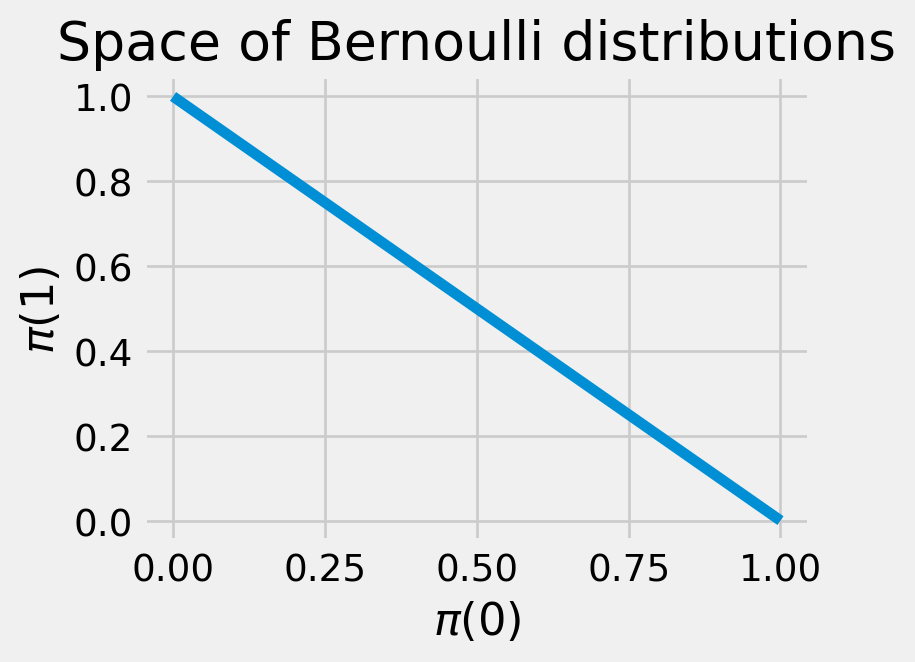
\includegraphics{bandits_files/figure-pdf/cell-10-output-1.pdf}

\section{Pure greedy}\label{sec-pure_greedy}

How might we improve on pure exploration? Instead, we could try each arm
once, and then commit to the one with the highest observed reward. We'll
call this the \textbf{pure greedy} strategy.

\begin{Shaded}
\begin{Highlighting}[]
\KeywordTok{class}\NormalTok{ PureGreedy(Agent):}
    \KeywordTok{def}\NormalTok{ choose\_arm(}\VariableTok{self}\NormalTok{):}
        \CommentTok{"""Choose the arm with the highest observed reward on its first pull."""}
        \ControlFlowTok{return}\NormalTok{ solutions.pure\_greedy\_choose\_arm(}\VariableTok{self}\NormalTok{)}
\end{Highlighting}
\end{Shaded}

Note we've used superscripts \(r^k\) during the exploration phase to
indicate that we observe exactly one reward for each arm. Then we use
subscripts \(r_t\) during the exploitation phase to indicate that we
observe a sequence of rewards from the chosen greedy arm \(\hat k\).

How does the expected regret of this strategy compare to that of pure
exploration? We'll do a more general analysis in the following section.
Now, for intuition, suppose there's just \(K=2\) arms, with Bernoulli
reward distributions with means \(\mu^0 > \mu^1\).

Let's let \(r^0\) be the random reward from the first arm and \(r^1\) be
the random reward from the second. If \(r^0 > r^1\), then we achieve
zero regret. Otherwise, we achieve regret \(T(\mu^0 - \mu^1)\). Thus,
the expected regret is simply:

\[
\begin{aligned}
    \mathbb{E}[\text{Regret}_T] &= \mathbb{P}(r^0 < r^1) \cdot T(\mu^0 - \mu^1) + c \\
    &= (1 - \mu^0) \mu^1 \cdot T(\mu^0 - \mu^1) + c
\end{aligned}
\]

Which is still \(\Theta(T)\), the same as pure exploration!

\begin{Shaded}
\begin{Highlighting}[]
\NormalTok{agent }\OperatorTok{=}\NormalTok{ PureGreedy(mab.K, mab.T)}
\NormalTok{mab\_loop(mab, agent)}
\NormalTok{plot\_strategy(mab, agent)}
\end{Highlighting}
\end{Shaded}

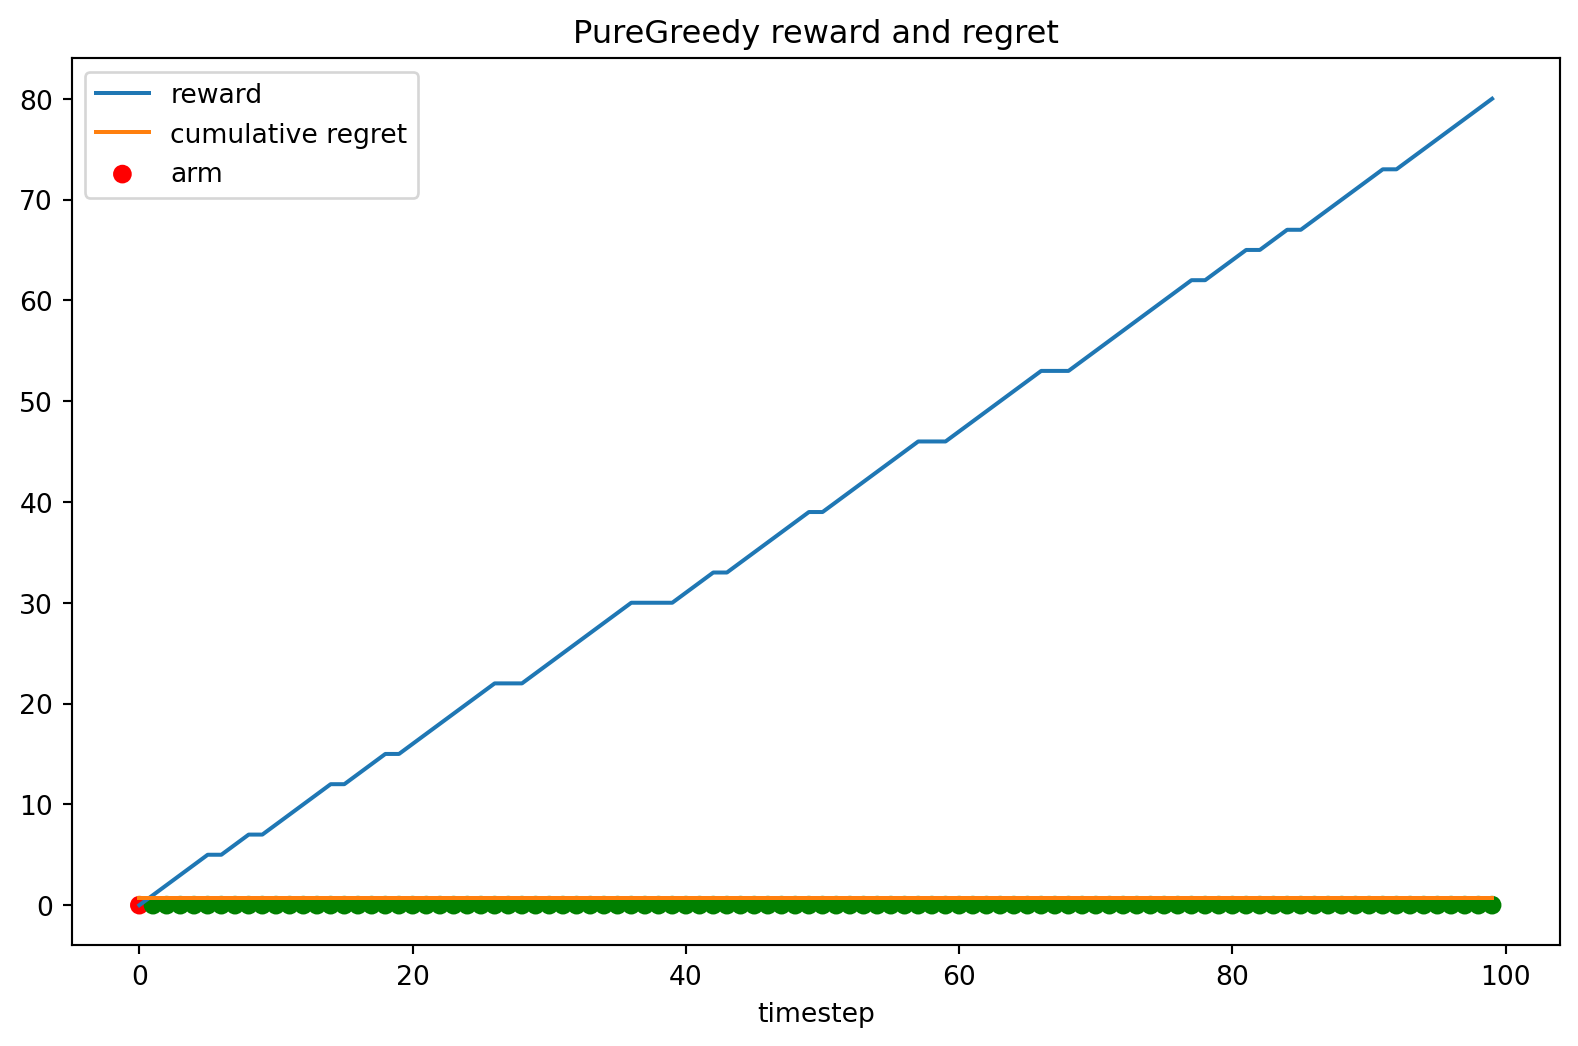
\includegraphics{bandits_files/figure-pdf/cell-12-output-1.pdf}

The cumulative regret is a straight line because the regret only depends
on the arms chosen and not the actual reward observed. In fact, if the
greedy algorithm happens to get lucky on the first set of pulls, it may
act entirely optimally for that episode! But its \emph{average} regret
is what measures its effectiveness.

\section{Explore-then-commit}\label{sec-etc}

We can improve the pure greedy algorithm as follows: let's reduce the
variance of the reward estimates by pulling each arm
\(N_{\text{explore}}> 1\) times before committing. This is called the
\textbf{explore-then-commit} strategy. Note that the ``pure greedy''
strategy above is just the special case where \(N_{\text{explore}}= 1\).

\begin{Shaded}
\begin{Highlighting}[]
\KeywordTok{class}\NormalTok{ ExploreThenCommit(Agent):}
    \KeywordTok{def} \FunctionTok{\_\_init\_\_}\NormalTok{(}\VariableTok{self}\NormalTok{, K: }\BuiltInTok{int}\NormalTok{, T: }\BuiltInTok{int}\NormalTok{, N\_explore: }\BuiltInTok{int}\NormalTok{):}
        \BuiltInTok{super}\NormalTok{().}\FunctionTok{\_\_init\_\_}\NormalTok{(K, T)}
        \VariableTok{self}\NormalTok{.N\_explore }\OperatorTok{=}\NormalTok{ N\_explore}

    \KeywordTok{def}\NormalTok{ choose\_arm(}\VariableTok{self}\NormalTok{):}
        \ControlFlowTok{return}\NormalTok{ solutions.etc\_choose\_arm(}\VariableTok{self}\NormalTok{)}
\end{Highlighting}
\end{Shaded}

\begin{Shaded}
\begin{Highlighting}[]
\NormalTok{agent }\OperatorTok{=}\NormalTok{ ExploreThenCommit(mab.K, mab.T, mab.T }\OperatorTok{//} \DecValTok{15}\NormalTok{)}
\NormalTok{mab\_loop(mab, agent)}
\NormalTok{plot\_strategy(mab, agent)}
\end{Highlighting}
\end{Shaded}

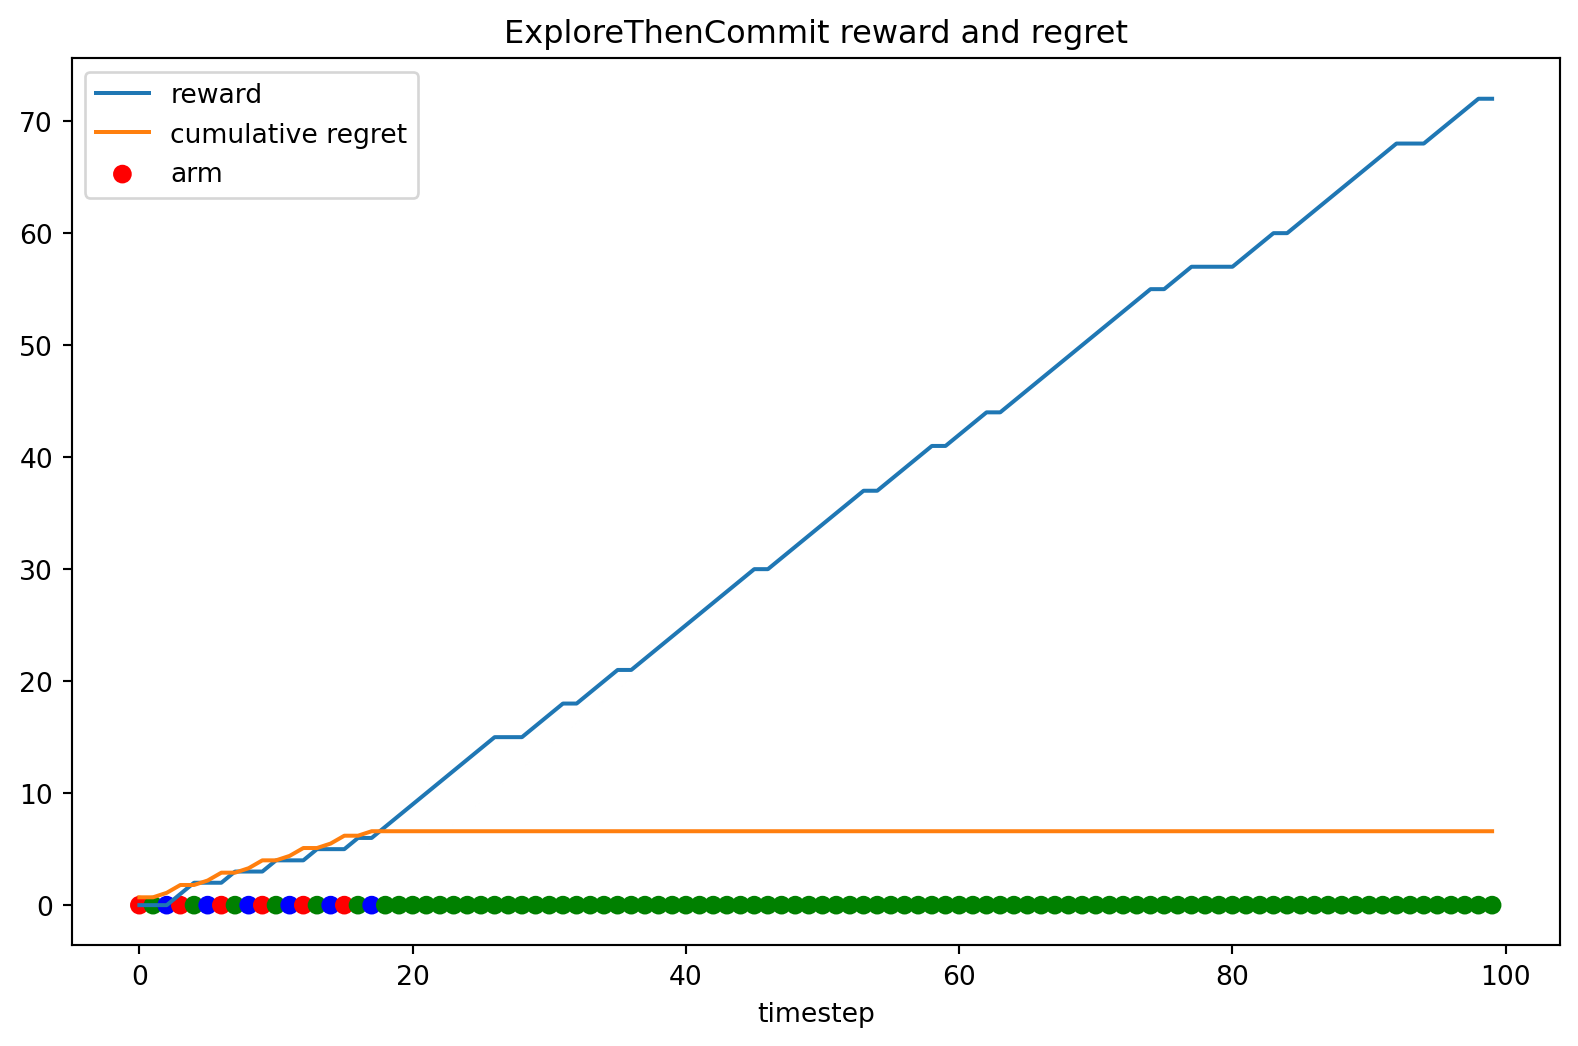
\includegraphics{bandits_files/figure-pdf/cell-14-output-1.pdf}

Notice that now, the graphs are much more consistent, and the algorithm
finds the true optimal arm and sticks with it much more frequently. We
would expect ETC to then have a better (i.e.~lower) average regret. Can
we prove this?

\subsection{ETC regret analysis}\label{sec-etc-regret-analysis}

Let's analyze the expected regret of the explore-then-commit strategy by
splitting it up into the exploration and exploitation phases.

\subsubsection{Exploration phase.}\label{exploration-phase.}

This phase takes \(N_{\text{explore}}K\) timesteps. Since at each step
we incur at most \(1\) regret, the total regret is at most
\(N_{\text{explore}}K\).

\subsubsection{Exploitation phase.}\label{exploitation-phase.}

This will take a bit more effort. We'll prove that for any total time
\(T\), we can choose \(N_{\text{explore}}\) such that with arbitrarily
high probability, the regret is sublinear.

Let \(\hat k\) denote the arm chosen after the exploration phase. We
know the regret from the exploitation phase is

\[T_{\text{exploit}} (\mu^\star - \mu^{\hat k}) \qquad \text{where} \qquad T_{\text{exploit}} := T - N_{\text{explore}}K.\]

So we'd like to bound \(\mu^\star - \mu^{\hat k} = o(1)\) (as a function
of \(T\)) in order to achieve sublinear regret. How can we do this?

Let's define \(\Delta^k = \hat \mu^k - \mu^k\) to denote how far the
mean estimate for arm \(k\) is from the true mean. How can we bound this
quantity? We'll use the following useful inequality for i.i.d. bounded
random variables:

\begin{theorem}[Hoeffding's
inequality]\protect\hypertarget{thm-hoeffding}{}\label{thm-hoeffding}

Let \(X_0, \dots, X_{n-1}\) be i.i.d. random variables with
\(X_i \in [0, 1]\) almost surely for each \(i \in [n]\). Then for any
\(\delta > 0\),

\[\mathbb{P}\left( \left| \frac{1}{n} \sum_{i=1}^n (X_i - \mathbb{E}[X_i]) \right| > \sqrt{\frac{\ln(2/\delta)}{2n}} \right) \le \delta.\]

\end{theorem}

The proof of this inequality is beyond the scope of this book. See
Vershynin (2018) Chapter 2.2.

We can apply this directly to the rewards for a given arm \(k\), since
the rewards from that arm are i.i.d.:

\begin{equation}\phantomsection\label{eq-hoeffding-etc}{
\mathbb{P}\left(|\Delta^k | > \sqrt{\frac{\ln(2/\delta)}{2N_{\text{explore}}}} \right) \le \delta.
}\end{equation}

But note that we can't apply this to arm \(\hat k\) directly since
\(\hat k\) is itself a random variable. Instead, we need to
``uniform-ize'' this bound across \emph{all} the arms, i.e.~bound the
error across all the arms simultaneously, so that the resulting bound
will apply \emph{no matter what} \(\hat k\) ``crystallizes'' to.

The \textbf{union bound} provides a simple way to do this:

\begin{theorem}[Union
bound]\protect\hypertarget{thm-union_bound}{}\label{thm-union_bound}

Consider a set of events \(A_0, \dots, A_{n-1}\). Then

\[\mathbb{P}(\exists i \in [n]. A_i) \le \sum_{i=0}^{n-1} \mathbb{P}(A_i).\]

In particular, if \(\mathbb{P}(A_i) \ge 1 - \delta\) for each
\(i \in [n]\), we have

\[\mathbb{P}(\forall i \in [n]. A_i) \ge 1 - n \delta.\]

\end{theorem}

\textbf{Exercise:} Prove the second statement above.

Applying the union bound across the arms for the l.h.s. event of
Equation~\ref{eq-hoeffding-etc}, we have

\[
\begin{aligned}
    \mathbb{P}\left( \forall k \in [K], |\Delta^k | \le \sqrt{\frac{\ln(2/\delta)}{2N_{\text{explore}}}} \right) &\ge 1-K\delta
\end{aligned}
\]

Then to apply this bound to \(\hat k\) in particular, we can apply the
useful trick of ``adding zero'':

\[
\begin{aligned}
    \mu^{k^\star} - \mu^{\hat k} &= \mu^{k^\star} - \mu^{\hat k} + (\hat \mu^{k^\star} - \hat \mu^{k^\star}) + (\hat \mu^{\hat k} - \hat \mu^{\hat k}) \\
    &= \Delta^{\hat k} - \Delta^{k^*} + \underbrace{(\hat \mu^{k^\star} - \hat \mu^{\hat k})}_{\le 0 \text{ by definition of } \hat k} \\
    &\le 2 \sqrt{\frac{\ln(2K/\delta')}{2N_{\text{explore}}}} \text{ with probability at least } 1-\delta'
\end{aligned}
\]

where we've set \(\delta' = K\delta\). Putting this all together, we've
shown that, with probability \(1 - \delta'\),

\[\text{Regret}_T \le N_{\text{explore}}K + T_{\text{exploit}} \cdot \sqrt{\frac{2\ln(2K/\delta')}{N_{\text{explore}}}}.\]

Note that it suffices for \(N_{\text{explore}}\) to be on the order of
\(\sqrt{T}\) to achieve sublinear regret. In particular, we can find the
optimal \(N_{\text{explore}}\) by setting the derivative of the r.h.s.
to zero:

\[
\begin{aligned}
    0 &= K - T_{\text{exploit}} \cdot \frac{1}{2} \sqrt{\frac{2\ln(2K/\delta')}{N_{\text{explore}}^3}} \\
    N_{\text{explore}}&= \left( T_{\text{exploit}} \cdot \frac{\sqrt{\ln(2K/\delta')/2}}{K} \right)^{2/3}
\end{aligned}
\]

Plugging this into the expression for the regret, we have (still with
probability \(1-\delta'\))

\[
\begin{aligned}
    \text{Regret}_T &\le 3 T^{2/3} \sqrt[3]{K \ln(2K/\delta') / 2} \\
    &= \tilde{O}(T^{2/3} K^{1/3}).
\end{aligned}
\]

The ETC algorithm is rather ``abrupt'' in that it switches from
exploration to exploitation after a fixed number of timesteps. In
practice, it's often better to use a more gradual transition, which
brings us to the \emph{epsilon-greedy} algorithm.

\section{Epsilon-greedy}\label{epsilon-greedy}

Instead of doing all of the exploration and then all of the exploitation
separately -- which additionally requires knowing the time horizon
beforehand -- we can instead interleave exploration and exploitation by,
at each timestep, choosing a random action with some probability. We
call this the \textbf{epsilon-greedy} algorithm.

\begin{Shaded}
\begin{Highlighting}[]
\KeywordTok{class}\NormalTok{ EpsilonGreedy(Agent):}
    \KeywordTok{def} \FunctionTok{\_\_init\_\_}\NormalTok{(}
        \VariableTok{self}\NormalTok{,}
\NormalTok{        K: }\BuiltInTok{int}\NormalTok{,}
\NormalTok{        T: }\BuiltInTok{int}\NormalTok{,}
\NormalTok{        ε\_array: Float[Array, }\StringTok{" T"}\NormalTok{],}
\NormalTok{    ):}
        \BuiltInTok{super}\NormalTok{().}\FunctionTok{\_\_init\_\_}\NormalTok{(K, T)}
        \VariableTok{self}\NormalTok{.ε\_array }\OperatorTok{=}\NormalTok{ ε\_array}

    \KeywordTok{def}\NormalTok{ choose\_arm(}\VariableTok{self}\NormalTok{):}
        \ControlFlowTok{return}\NormalTok{ solutions.epsilon\_greedy\_choose\_arm(}\VariableTok{self}\NormalTok{)}
\end{Highlighting}
\end{Shaded}

\begin{Shaded}
\begin{Highlighting}[]
\NormalTok{agent }\OperatorTok{=}\NormalTok{ EpsilonGreedy(mab.K, mab.T, np.full(mab.T, }\FloatTok{0.1}\NormalTok{))}
\NormalTok{mab\_loop(mab, agent)}
\NormalTok{plot\_strategy(mab, agent)}
\end{Highlighting}
\end{Shaded}

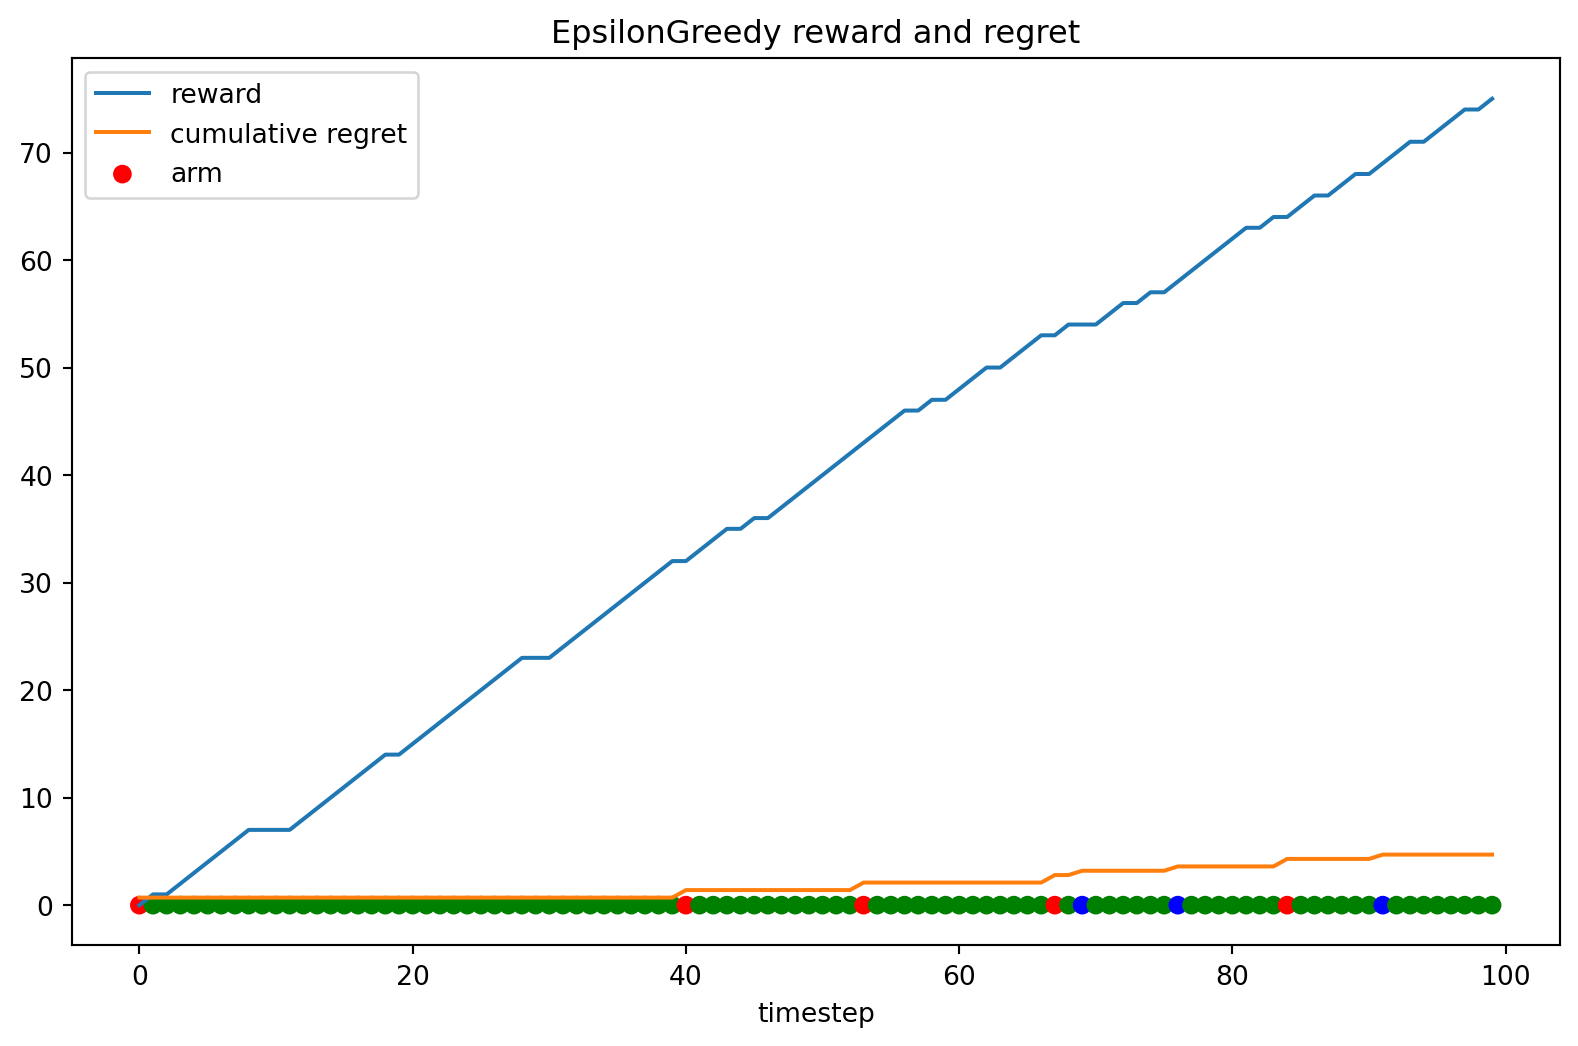
\includegraphics{bandits_files/figure-pdf/cell-16-output-1.pdf}

Note that we let \(\epsilon\) vary over time. In particular, we might
want to gradually \emph{decrease} \(\epsilon\) as we learn more about
the reward distributions and no longer need to spend time exploring.

What is the expected regret of the algorithm if we set \(\epsilon\) to
be a constant?

It turns out that setting \(\epsilon_t = \sqrt[3]{K \ln(t)/t}\) also
achieves a regret of \(\tilde O(t^{2/3} K^{1/3})\) (ignoring the
logarithmic factors). (We will not prove this here; a proof can be found
in Agarwal et al. (2022).)

In ETC, we had to set \(N_{\text{explore}}\) based on the total number
of timesteps \(T\). But the epsilon-greedy algorithm actually handles
the exploration \emph{automatically}: the regret rate holds for
\emph{any} \(t\), and doesn't depend on the final horizon \(T\).

But the way these algorithms explore is rather naive: we've been
exploring \emph{uniformly} across all the arms. But what if we could be
smarter about it, and explore \emph{more} for arms that we're less
certain about?

\section{Upper Confidence Bound (UCB)}\label{sec-ucb}

To quantify how \emph{certain} we are about the mean of each arm, we'll
compute \emph{confidence intervals} for our estimators, and then choose
the arm with the highest \emph{upper confidence bound}. This operates on
the principle of \textbf{the benefit of the doubt (i.e.~optimism in the
face of uncertainty)}: we'll choose the arm that we're most optimistic
about.

In particular, for each arm \(k\) at time \(t\), we'd like to compute
some upper confidence bound \(M^k_t\) such that
\(\hat \mu^k_t \le M^k_t\) with high probability, and then choose
\(a_t := \arg \max_{k \in [K]} M^k_t\). But how should we compute
\(M^k_t\)?

In Section~\ref{sec-etc-regret-analysis}, we were able to compute this
bound using Hoeffding's inequality, which assumes that the number of
samples is \emph{fixed}. This was the case in ETC (where we pull each
arm \(N_{\text{explore}}\) times), but in UCB, the number of times we
pull each arm depends on the agent's actions, which in turn depend on
the random rewards and are therefore stochastic. So we \emph{can't} use
Hoeffding's inequality directly.

Instead, we'll apply the same trick we used in the ETC analysis: we'll
use the \textbf{union bound} to compute a \emph{looser} bound that holds
\emph{uniformly} across all timesteps and arms. Let's introduce some
notation to discuss this.

Let \(N^k_t\) denote the (random) number of times arm \(k\) has been
pulled within the first \(t\) timesteps, and \(\hat \mu^k_t\) denote the
sample average of those pulls. That is,

\[
\begin{aligned}
    N^k_t &:= \sum_{\tau=0}^{t-1} \mathbf{1} \{ a_\tau = k \} \\
    \hat \mu^k_t &:= \frac{1}{N^k_t} \sum_{\tau=0}^{t-1} \mathbf{1} \{ a_\tau = k \} r_\tau.
\end{aligned}
\]

To achieve the ``fixed sample size'' assumption, we'll need to shift our
index from \emph{time} to \emph{number of samples from each arm}. In
particular, we'll define \(\tilde r^k_n\) to be the \(n\)th sample from
arm \(k\), and \(\tilde \mu^k_n\) to be the sample average of the first
\(n\) samples from arm \(k\). Then, for a fixed \(n\), this satisfies
the ``fixed sample size'' assumption, and we can apply Hoeffding's
inequality to get a bound on \(\tilde \mu^k_n\).

So how can we extend our bound on \(\tilde\mu^k_n\) to \(\hat \mu^k_t\)?
Well, we know \(N^k_t \le t\) (where equality would be the case if and
only if we had pulled arm \(k\) every time). So we can apply the same
trick as last time, where we uniform-ize across all possible values of
\(N^k_t\):

\[
\begin{aligned}
    \mathbb{P}\left( \forall n \le t, |\tilde \mu^k_n - \mu^k | \le \sqrt{\frac{\ln(2/\delta)}{2n}} \right) &\ge 1-t\delta.
\end{aligned}
\]

In particular, since \(N^k_t \le t\), and
\(\tilde \mu^k_{N^k_t} = \hat \mu^k_t\) by definition, we have

\[
\begin{aligned}
    \mathbb{P}\left( |\hat \mu^k_t - \mu^k | \le \sqrt{\frac{\ln(2t/\delta')}{2N^k_t}} \right) &\ge 1-\delta' \text{ where } \delta' := t \delta.
\end{aligned}
\]

This bound would then suffice for applying the UCB algorithm! That is,
the upper confidence bound for arm \(k\) would be

\[M^k_t := \hat \mu^k_t + \sqrt{\frac{\ln(2t/\delta')}{2N^k_t}},\]

where we can choose \(\delta'\) depending on how tight we want the
interval to be.

\begin{itemize}
\tightlist
\item
  A smaller \(\delta'\) would give us a larger and higher-confidence
  interval, emphasizing the exploration term.
\item
  A larger \(\delta'\) would give a tighter and lower-confidence
  interval, prioritizing the current sample averages.
\end{itemize}

We can now use this to define the UCB algorithm.

\begin{Shaded}
\begin{Highlighting}[]
\KeywordTok{class}\NormalTok{ UCB(Agent):}
    \KeywordTok{def} \FunctionTok{\_\_init\_\_}\NormalTok{(}\VariableTok{self}\NormalTok{, K: }\BuiltInTok{int}\NormalTok{, T: }\BuiltInTok{int}\NormalTok{, delta: }\BuiltInTok{float}\NormalTok{):}
        \BuiltInTok{super}\NormalTok{().}\FunctionTok{\_\_init\_\_}\NormalTok{(K, T)}
        \VariableTok{self}\NormalTok{.delta }\OperatorTok{=}\NormalTok{ delta}

    \KeywordTok{def}\NormalTok{ choose\_arm(}\VariableTok{self}\NormalTok{):}
        \ControlFlowTok{return}\NormalTok{ solutions.ucb\_choose\_arm(}\VariableTok{self}\NormalTok{)}
\end{Highlighting}
\end{Shaded}

Intuitively, UCB prioritizes arms where:

\begin{enumerate}
\def\labelenumi{\arabic{enumi}.}
\item
  \(\hat \mu^k_t\) is large, i.e.~the arm has a high sample average, and
  we'd choose it for \emph{exploitation}, and
\item
  \(\sqrt{\frac{\ln(2t/\delta')}{2N^k_t}}\) is large, i.e.~we're still
  uncertain about the arm, and we'd choose it for \emph{exploration}.
\end{enumerate}

As desired, this explores in a smarter, \emph{adaptive} way compared to
the previous algorithms. Does it achieve lower regret?

\begin{Shaded}
\begin{Highlighting}[]
\NormalTok{agent }\OperatorTok{=}\NormalTok{ UCB(mab.K, mab.T, }\FloatTok{0.9}\NormalTok{)}
\NormalTok{mab\_loop(mab, agent)}
\NormalTok{plot\_strategy(mab, agent)}
\end{Highlighting}
\end{Shaded}

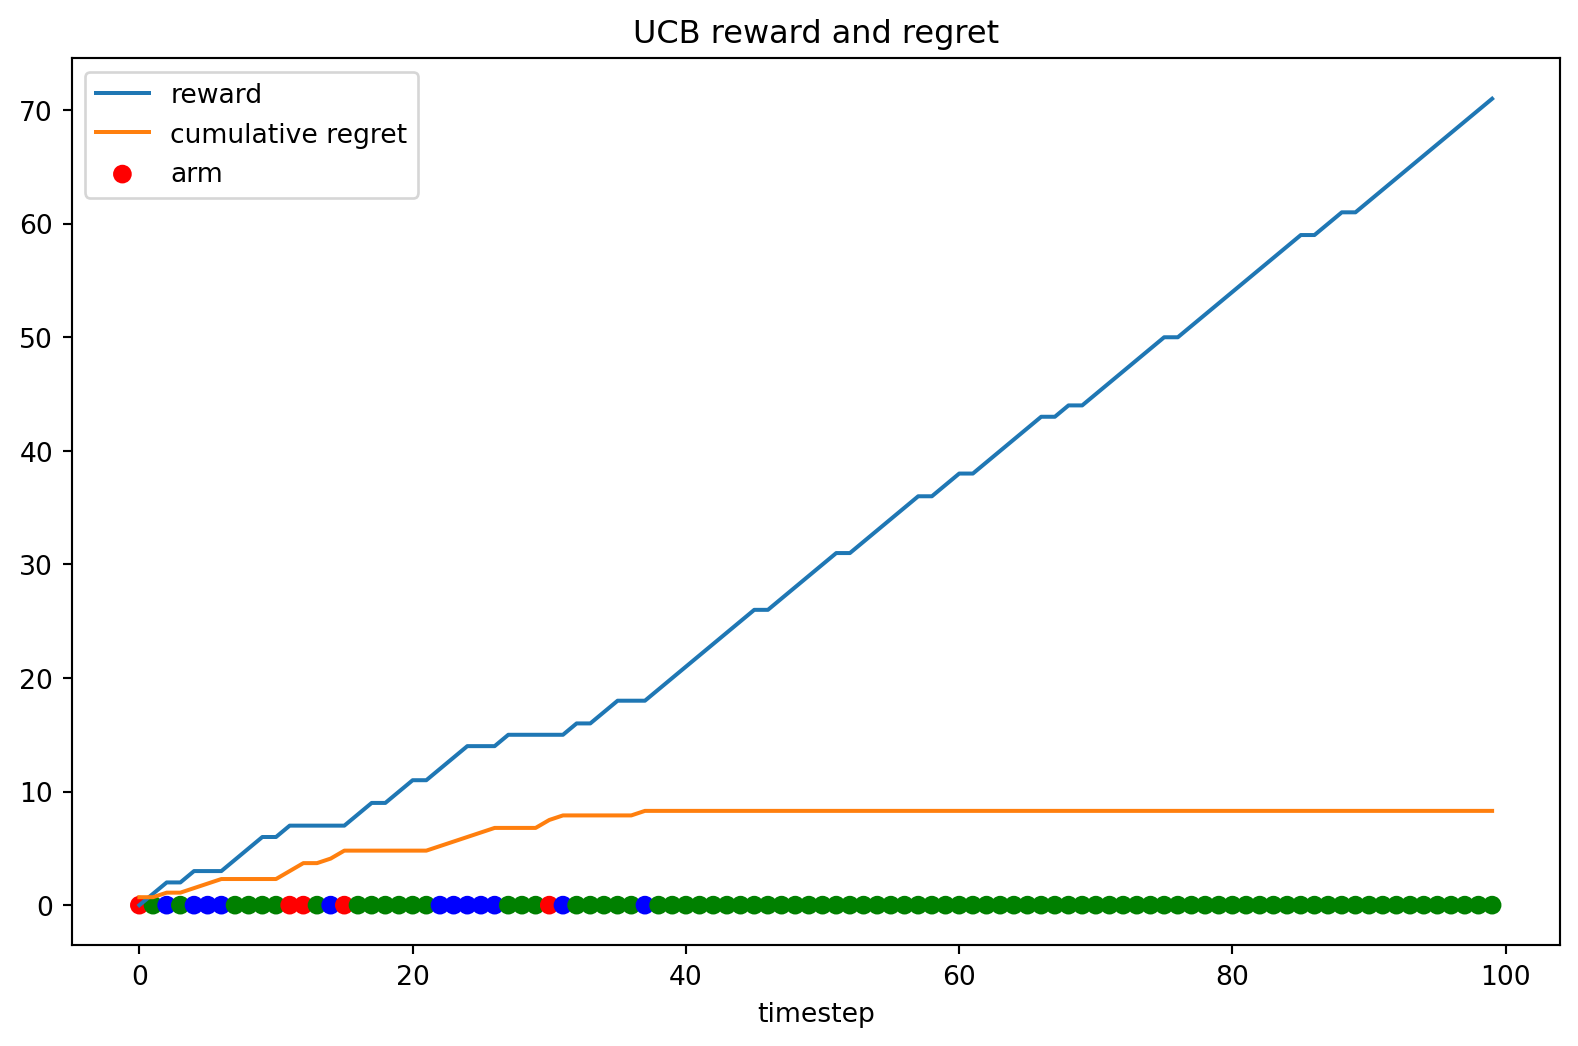
\includegraphics{bandits_files/figure-pdf/cell-18-output-1.pdf}

\subsection{UCB regret analysis}\label{ucb-regret-analysis}

First we'll bound the regret incurred at each timestep. Then we'll bound
the \emph{total} regret across timesteps.

For the sake of analysis, we'll use a slightly looser bound that applies
across the whole time horizon and across all arms. We'll omit the
derivation since it's very similar to the above (walk through it
yourself for practice).

\[
\begin{aligned}
    \mathbb{P}\left(\forall k \le K, t < T. |\hat \mu^k_t - \mu^k | \le B^k_t \right) &\ge 1-\delta'' \\
    \text{where} \quad B^k_t &:= \sqrt{\frac{\ln(2TK/\delta'')}{2N^k_t}}.
\end{aligned}
\]

Intuitively, \(B^k_t\) denotes the \emph{width} of the CI for arm \(k\)
at time \(t\). Then, assuming the above uniform bound holds (which
occurs with probability \(1-\delta''\)), we can bound the regret at each
timestep as follows:

\[
\begin{aligned}
    \mu^\star - \mu^{a_t} &\le \hat \mu^{k^*}_t + B_t^{k^*} - \mu^{a_t} && \text{applying UCB to arm } k^\star \\
    &\le \hat \mu^{a_t}_t + B^{a_t}_t - \mu^{a_t} && \text{since UCB chooses } a_t = \arg \max_{k \in [K]} \hat \mu^k_t + B_t^{k} \\
    &\le 2 B^{a_t}_t && \text{since } \hat \mu^{a_t}_t - \mu^{a_t} \le B^{a_t}_t \text{ by definition of } B^{a_t}_t \\
\end{aligned}
\]

Summing this across timesteps gives

\[
\begin{aligned}
    \text{Regret}_T &\le \sum_{t=0}^{T-1} 2 B^{a_t}_t \\
    &= \sqrt{2\ln(2TK/\delta'')} \sum_{t=0}^{T-1} (N^{a_t}_t)^{-1/2} \\
    \sum_{t=0}^{T-1} (N^{a_t}_t)^{-1/2} &= \sum_{t=0}^{T-1} \sum_{k=1}^K \mathbf{1}\{ a_t = k \} (N^k_t)^{-1/2} \\
    &= \sum_{k=1}^K \sum_{n=1}^{N_T^k} n^{-1/2} \\
    &\le K \sum_{n=1}^T n^{-1/2} \\
    \sum_{n=1}^T n^{-1/2} &\le 1 + \int_1^T x^{-1/2} \ \mathrm{d}x \\
    &= 1 + (2 \sqrt{x})_1^T \\
    &= 2 \sqrt{T} - 1 \\
    &\le 2 \sqrt{T} \\
\end{aligned}
\]

Putting everything together gives

\[
\begin{aligned}
    \text{Regret}_T &\le 2 K \sqrt{2T \ln(2TK/\delta'')} && \text{with probability } 1-\delta'' \\
    &= \tilde O(K\sqrt{T})
\end{aligned}
\]

In fact, we can do a more sophisticated analysis to trim off a factor of
\(\sqrt{K}\) and show \(\text{Regret}_T = \tilde O(\sqrt{TK})\).

\subsection{Lower bound on regret
(intuition)}\label{lower-bound-on-regret-intuition}

Is it possible to do better than \(\Omega(\sqrt{T})\) in general? In
fact, no! We can show that any algorithm must incur \(\Omega(\sqrt{T})\)
regret in the worst case. We won't rigorously prove this here, but the
intuition is as follows.

The Central Limit Theorem tells us that with \(T\) i.i.d. samples from
some distribution, we can only learn the mean of the distribution to
within \(\Omega(1/\sqrt{T})\) (the standard deviation). Then, since we
get \(T\) samples spread out across the arms, we can only learn each
arm's mean to an even looser degree.

That is, if two arms have means that are within about \(1/\sqrt{T}\), we
won't be able to confidently tell them apart, and will sample them about
equally. But then we'll incur regret
\[\Omega((T/2) \cdot (1/\sqrt{T})) = \Omega(\sqrt{T}).\]

\section{Thompson sampling and Bayesian
bandits}\label{sec-thompson_sampling}

So far, we've treated the parameters \(\mu^0, \dots, \mu^{K-1}\) of the
reward distributions as \emph{fixed}. Instead, we can take a
\textbf{Bayesian} approach where we treat them as random variables from
some \textbf{prior distribution}. Then, upon pulling an arm and
observing a reward, we can simply \emph{condition} on this observation
to exactly describe the \textbf{posterior distribution} over the
parameters. This fully describes the information we gain about the
parameters from observing the reward.

From this Bayesian perspective, the \textbf{Thompson sampling} algorithm
follows naturally: just sample from the distribution of the optimal arm,
given the observations!

\begin{Shaded}
\begin{Highlighting}[]
\KeywordTok{class}\NormalTok{ Distribution:}
    \KeywordTok{def}\NormalTok{ sample(}\VariableTok{self}\NormalTok{) }\OperatorTok{{-}\textgreater{}}\NormalTok{ Float[Array, }\StringTok{" K"}\NormalTok{]:}
        \CommentTok{"""Sample a vector of means for the K arms."""}
\NormalTok{        ...}

    \KeywordTok{def}\NormalTok{ update(}\VariableTok{self}\NormalTok{, arm: }\BuiltInTok{int}\NormalTok{, reward: }\BuiltInTok{float}\NormalTok{):}
        \CommentTok{"""Condition on obtaining \textasciigrave{}reward\textasciigrave{} from the given arm."""}
\NormalTok{        ...}
\end{Highlighting}
\end{Shaded}

\begin{Shaded}
\begin{Highlighting}[]
\KeywordTok{class}\NormalTok{ ThompsonSampling(Agent):}
    \KeywordTok{def} \FunctionTok{\_\_init\_\_}\NormalTok{(}\VariableTok{self}\NormalTok{, K: }\BuiltInTok{int}\NormalTok{, T: }\BuiltInTok{int}\NormalTok{, prior: Distribution):}
        \BuiltInTok{super}\NormalTok{().}\FunctionTok{\_\_init\_\_}\NormalTok{(K, T)}
        \VariableTok{self}\NormalTok{.distribution }\OperatorTok{=}\NormalTok{ prior}

    \KeywordTok{def}\NormalTok{ choose\_arm(}\VariableTok{self}\NormalTok{):}
\NormalTok{        means }\OperatorTok{=} \VariableTok{self}\NormalTok{.distribution.sample()}
        \ControlFlowTok{return}\NormalTok{ random\_argmax(means)}

    \KeywordTok{def}\NormalTok{ update\_history(}\VariableTok{self}\NormalTok{, arm: }\BuiltInTok{int}\NormalTok{, reward: }\BuiltInTok{int}\NormalTok{):}
        \BuiltInTok{super}\NormalTok{().update\_history(arm, reward)}
        \VariableTok{self}\NormalTok{.distribution.update(arm, reward)}
\end{Highlighting}
\end{Shaded}

In other words, we sample each arm proportionally to how likely we think
it is to be optimal, given the observations so far. This strikes a good
exploration-exploitation tradeoff: we explore more for arms that we're
less certain about, and exploit more for arms that we're more certain
about. Thompson sampling is a simple yet powerful algorithm that
achieves state-of-the-art performance in many settings.

\begin{example}[Bayesian Bernoulli
bandit]\protect\hypertarget{exm-bayesian_bernoulli}{}\label{exm-bayesian_bernoulli}

We've been working in the Bernoulli bandit setting, where arm \(k\)
yields a reward of \(1\) with probability \(\mu^k\) and no reward
otherwise. The vector of success probabilities
\(\boldsymbol{\mu} = (\mu^1, \dots, \mu^K)\) thus describes the entire
MAB.

Under the Bayesian perspective, we think of \(\boldsymbol{\mu}\) as a
\emph{random} vector drawn from some prior distribution
\(\pi(\boldsymbol{\mu})\). For example, we might have \(\pi\) be the
Uniform distribution over the unit hypercube \([0, 1]^K\), that is,

\[\pi(\boldsymbol{\mu}) = \begin{cases}
    1 & \text{if } \boldsymbol{\mu}\in [0, 1]^K \\
    0 & \text{otherwise}
\end{cases}\]

In this case, upon viewing some reward, we can exactly calculate the
\textbf{posterior} distribution of \(\boldsymbol{\mu}\) using Bayes's
rule (i.e.~the definition of conditional probability):

\[
\begin{aligned}
    \mathbb{P}(\boldsymbol{\mu} \mid a_0, r_0) &\propto \mathbb{P}(r_0 \mid a_0, \boldsymbol{\mu}) \mathbb{P}(a_0 \mid \boldsymbol{\mu}) \mathbb{P}(\boldsymbol{\mu}) \\
    &\propto (\mu^{a_0})^{r_0} (1 - \mu^{a_0})^{1-r_0}.
\end{aligned}
\]

This is the PDF of the \(\text{Beta}(1 + r_0, 1 + (1 - r_0))\)
distribution, which is a conjugate prior for the Bernoulli distribution.
That is, if we start with a Beta prior on \(\mu^k\) (note that
\(\text{Unif}([0, 1]) = \text{Beta}(1, 1)\)), then the posterior, after
conditioning on samples from \(\text{Bern}(\mu^k)\), will also be Beta.
This is a very convenient property, since it means we can simply update
the parameters of the Beta distribution upon observing a reward, rather
than having to recompute the entire posterior distribution from scratch.

\end{example}

\begin{Shaded}
\begin{Highlighting}[]
\KeywordTok{class}\NormalTok{ Beta(Distribution):}
    \KeywordTok{def} \FunctionTok{\_\_init\_\_}\NormalTok{(}\VariableTok{self}\NormalTok{, K: }\BuiltInTok{int}\NormalTok{, alpha: }\BuiltInTok{int} \OperatorTok{=} \DecValTok{1}\NormalTok{, beta: }\BuiltInTok{int} \OperatorTok{=} \DecValTok{1}\NormalTok{):}
        \VariableTok{self}\NormalTok{.alphas }\OperatorTok{=}\NormalTok{ np.full(K, alpha)}
        \VariableTok{self}\NormalTok{.betas }\OperatorTok{=}\NormalTok{ np.full(K, beta)}

    \KeywordTok{def}\NormalTok{ sample(}\VariableTok{self}\NormalTok{):}
        \ControlFlowTok{return}\NormalTok{ np.random.beta(}\VariableTok{self}\NormalTok{.alphas, }\VariableTok{self}\NormalTok{.betas)}

    \KeywordTok{def}\NormalTok{ update(}\VariableTok{self}\NormalTok{, arm: }\BuiltInTok{int}\NormalTok{, reward: }\BuiltInTok{int}\NormalTok{):}
        \VariableTok{self}\NormalTok{.alphas[arm] }\OperatorTok{+=}\NormalTok{ reward}
        \VariableTok{self}\NormalTok{.betas[arm] }\OperatorTok{+=} \DecValTok{1} \OperatorTok{{-}}\NormalTok{ reward}
\end{Highlighting}
\end{Shaded}

\begin{Shaded}
\begin{Highlighting}[]
\NormalTok{beta\_distribution }\OperatorTok{=}\NormalTok{ Beta(mab.K)}
\NormalTok{agent }\OperatorTok{=}\NormalTok{ ThompsonSampling(mab.K, mab.T, beta\_distribution)}
\NormalTok{mab\_loop(mab, agent)}
\NormalTok{plot\_strategy(mab, agent)}
\end{Highlighting}
\end{Shaded}

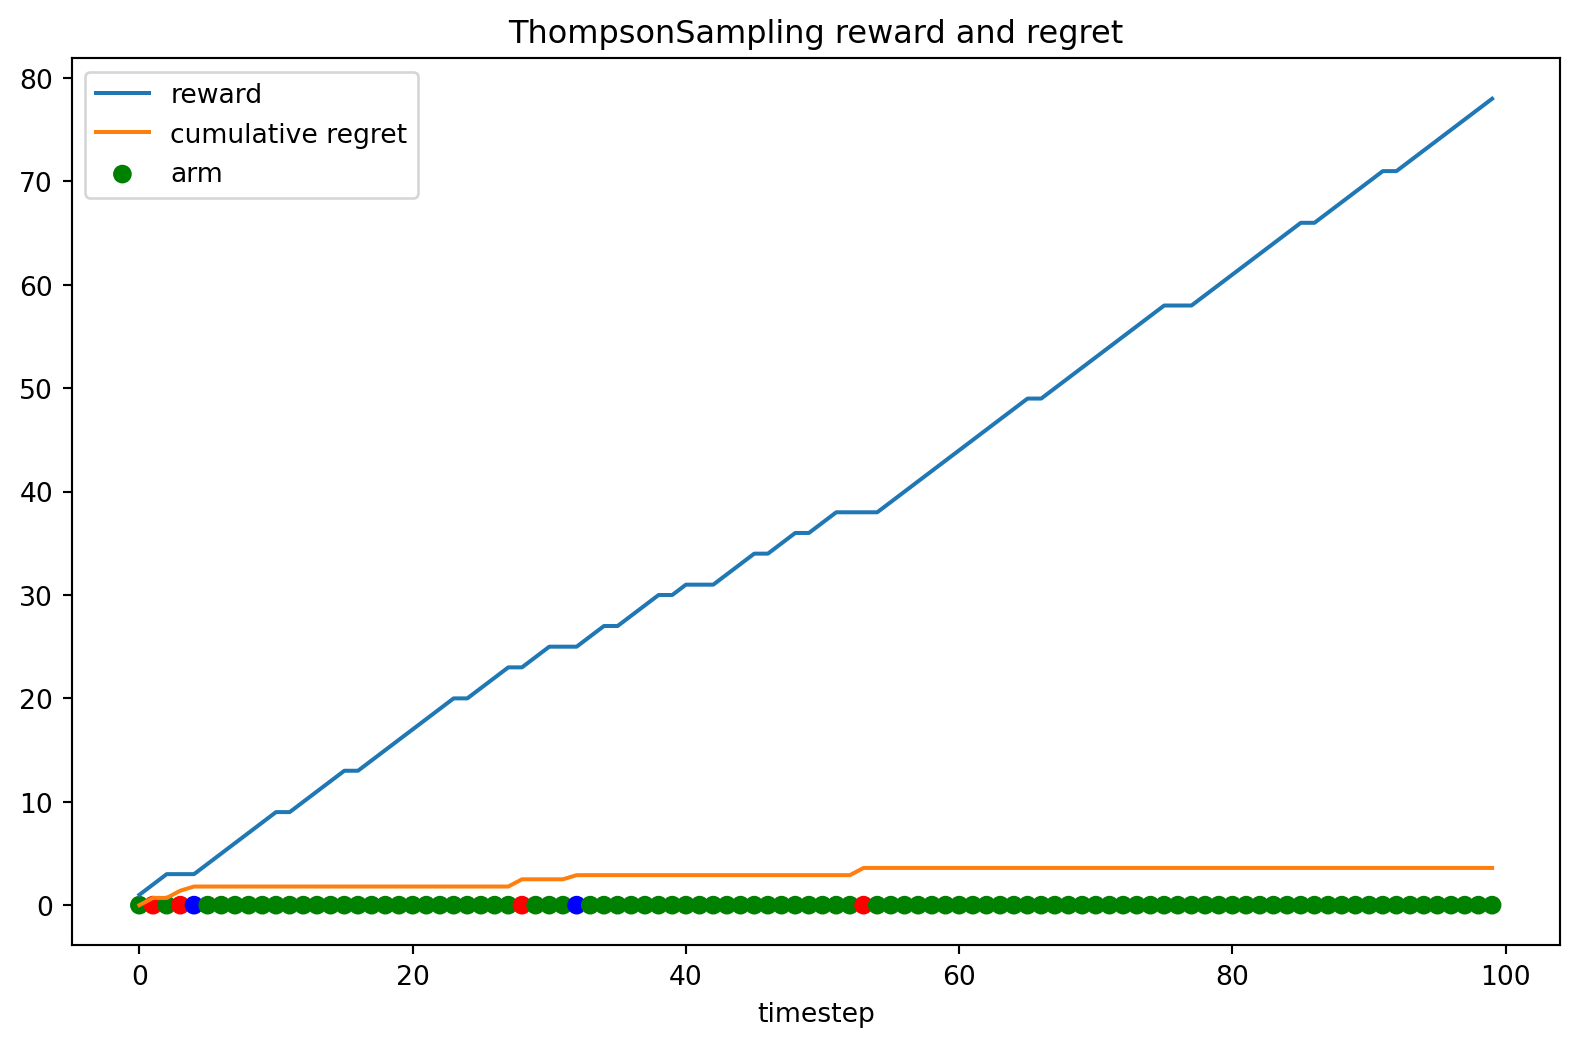
\includegraphics{bandits_files/figure-pdf/cell-22-output-1.pdf}

It turns out that asymptotically, Thompson sampling is optimal in the
following sense. Lai and Robbins (1985) prove an
\emph{instance-dependent} lower bound that says for \emph{any} bandit
algorithm,

\[\liminf_{T \to \infty} \frac{\mathbb{E}[N_T^k]}{\ln(T)} \ge \frac{1}{\text{KL}(\mu^k \parallel \mu^\star)}\]

where

\[\text{KL}(\mu^k \parallel \mu^\star) = \mu^k \ln \frac{\mu^k}{\mu^\star} + (1 - \mu^k) \ln \frac{1 - \mu^k}{1 - \mu^\star}\]

measures the \textbf{Kullback-Leibler divergence} from the Bernoulli
distribution with mean \(\mu^k\) to the Bernoulli distribution with mean
\(\mu^\star\). It turns out that Thompson sampling achieves this lower
bound with equality! That is, not only is the error \emph{rate} optimal,
but the \emph{constant factor} is optimal as well.

\section{Contextual bandits}\label{contextual-bandits}

This content is advanced material taught at the end of the course.

In the above MAB environment, the reward distributions of the arms
remain constant. However, in many real-world settings, we might receive
additional information that affects these distributions. For example, in
the online advertising case where each arm corresponds to an ad we could
show the user, we might receive information about the user's preferences
that changes how likely they are to click on a given ad. We can model
such environments using \textbf{contextual bandits}.

\begin{definition}[Contextual
bandit]\protect\hypertarget{def-contextual_bandit}{}\label{def-contextual_bandit}

At each timestep \(t\), a new \emph{context} \(x_t\) is drawn from some
distribution \(\nu_{\text{x}}\). The learner gets to observe the
context, and choose an action \(a_t\) according to some
context-dependent policy \(\pi_t(x_t)\). Then, the learner observes the
reward from the chosen arm \(r_t \sim \nu^{a_t}(x_t)\). The reward
distribution also depends on the context.

\end{definition}

Assuming our context is \emph{discrete}, we can just perform the same
algorithms, treating each context-arm pair as its own arm. This gives us
an enlarged MAB of \(K |\mathcal{X}|\) arms.

Write down the UCB algorithm for this enlarged MAB. That is, write an
expression for \(\pi_t(x_t) = \arg\max_a \dots\).

Recall that running UCB for \(T\) timesteps on an MAB with \(K\) arms
achieves a regret bound of \(\tilde{O}(\sqrt{TK})\). So in this problem,
we would achieve regret \(\tilde{O}(\sqrt{TK|\mathcal{X}|})\) in the
contextual MAB, which has a polynomial dependence on \(|\mathcal{X}|\).
But in a situation where we have large, or even infinitely many
contexts, e.g.~in the case where our context is a continuous value, this
becomes intractable.

Note that this ``enlarged MAB'' treats the different contexts as
entirely unrelated to each other, while in practice, often contexts are
\emph{related} to each other in some way: for example, we might want to
advertise similar products to users with similar preferences. How can we
incorporate this structure into our solution?

\subsection{Linear contextual bandits}\label{sec-lin_ucb}

We want to model the \emph{mean reward} of arm \(k\) as a function of
the context, i.e.~\(\mu^k(x)\). One simple model is the \emph{linear}
one: \(\mu^k(x) = x^\top \theta^k\), where
\(x \in \mathcal{X} = \mathbb{R}^d\) and \(\theta^k \in \mathbb{R}^d\)
describes a \emph{feature direction} for arm \(k\). Recall that
\textbf{supervised learning} gives us a way to estimate a conditional
expectation from samples: We learn a \emph{least squares} estimator from
the timesteps where arm \(k\) was selected:
\[\hat \theta_t^k = \arg\min_{\theta \in \mathbb{R}^d} \sum_{\{ i \in [t] : a_i = k \}} (r_i - x_i^\top \theta)^2.\]
This has the closed-form solution known as the \emph{ordinary least
squares} (OLS) estimator:

\begin{equation}\phantomsection\label{eq-ols_bandit}{
\begin{aligned}
    \hat \theta_t^k          & = (A_t^k)^{-1} \sum_{\{ i \in [t] : a_i = k \}} x_i r_i \\
    \text{where} \quad A_t^k & = \sum_{\{ i \in [t] : a_i = k \}} x_i x_i^\top.
\end{aligned}
}\end{equation}

We can now apply the UCB algorithm in this environment in order to
balance \emph{exploration} of new arms and \emph{exploitation} of arms
that we believe to have high reward. But how should we construct the
upper confidence bound? Previously, we treated the pulls of an arm as
i.i.d. samples and used Hoeffding's inequality to bound the distance of
the sample mean, our estimator, from the true mean. However, now our
estimator is not a sample mean, but rather the OLS estimator above
Equation~\ref{eq-ols_bandit}. Instead, we'll use \textbf{Chebyshev's
inequality} to construct an upper confidence bound.

\begin{theorem}[Chebyshev's
inequality]\protect\hypertarget{thm-chebyshev}{}\label{thm-chebyshev}

For a random variable \(Y\) such that \(\mathbb{E}Y = 0\) and
\(\mathbb{E}Y^2 = \sigma^2\),
\[|Y| \le \beta \sigma \quad \text{with probability} \ge 1 - \frac{1}{\beta^2}\]

\end{theorem}

Since the OLS estimator is known to be unbiased (try proving this
yourself), we can apply Chebyshev's inequality to
\(x_t^\top (\hat \theta_t^k - \theta^k)\):

\[\begin{aligned}
    x_t^\top \theta^k \le x_t^\top \hat \theta_t^k + \beta \sqrt{x_t^\top (A_t^k)^{-1} x_t} \quad \text{with probability} \ge 1 - \frac{1}{\beta^2}
\end{aligned}\]

We haven't explained why \(x_t^\top (A_t^k)^{-1} x_t\) is the correct
expression for the variance of \(x_t^\top \hat \theta_t^k\). This result
follows from some algebra on the definition of the OLS estimator
Equation~\ref{eq-ols_bandit}.

The first term is exactly our predicted reward \(\hat \mu^k_t(x_t)\). To
interpret the second term, note that
\[x_t^\top (A_t^k)^{-1} x_t = \frac{1}{N_t^k} x_t^\top (\Sigma_t^k)^{-1} x_t,\]
where
\[\Sigma_t^k = \frac{1}{N_t^k} \sum_{\{ i \in [t] : a_i = k \}} x_i x_i^\top\]
is the empirical covariance matrix of the contexts (assuming that the
context has mean zero). That is, the learner is encouraged to choose
arms when \(x_t\) is \emph{not aligned} with the data seen so far, or if
arm \(k\) has not been explored much and so \(N_t^k\) is small.

We can now substitute these quantities into UCB to get the
\textbf{LinUCB} algorithm:

\begin{Shaded}
\begin{Highlighting}[]
\NormalTok{class LinUCBPseudocode(Agent):}
\NormalTok{    def \_\_init\_\_(}
\NormalTok{        self, K: int, T: int, D: int, lam: float, get\_c: Callable[[int], float]}
\NormalTok{    ):}
\NormalTok{        super().\_\_init\_\_(K, T)}
\NormalTok{        self.lam = lam}
\NormalTok{        self.get\_c = get\_c}
\NormalTok{        self.contexts = [None for \_ in range(K)]}
\NormalTok{        self.A = np.repeat(lam * np.eye(D)[...], K)  \# regularization}
\NormalTok{        self.targets = np.zeros(K, D)}
\NormalTok{        self.w = np.zeros(K, D)}

\NormalTok{    def choose\_arm(self, context: Float[Array, " D"]):}
\NormalTok{        c = self.get\_c(self.count)}
\NormalTok{        scores = self.w @ context + c * np.sqrt(}
\NormalTok{            context.T @ np.linalg.solve(self.A, context)}
\NormalTok{        )}
\NormalTok{        return random\_argmax(scores)}

\NormalTok{    def update\_history(self, context: Float[Array, " D"], arm: int, reward: int):}
\NormalTok{        self.A[arm] += np.outer(context, context)}
\NormalTok{        self.targets[arm] += context * reward}
\NormalTok{        self.w[arm] = np.linalg.solve(self.A[arm], self.targets[arm])}
\end{Highlighting}
\end{Shaded}

Note that the matrix \(A_t^k\) above might not be invertible. When does
this occur? One way to address this is to include a \(\lambda I\)
regularization term to ensure that \(A_t^k\) is invertible. This is
equivalent to solving a \emph{ridge regression} problem instead of the
unregularized least squares problem. Implement this solution.

\(c_t\) is similar to the \(\log (2t/\delta')\) term of UCB: It controls
the width of the confidence interval. Here, we treat it as a tunable
parameter, though in a theoretical analysis, it would depend on
\(A_t^k\) and the probability \(\delta\) with which the bound holds.

Using similar tools for UCB, we can also prove an
\(\tilde{O}(\sqrt{T})\) regret bound. The full details of the analysis
can be found in Section 3 of Agarwal et al. (2022).

\section{Summary}\label{summary-2}

In this chapter, we explored the \textbf{multi-armed bandit} setting for
analyzing sequential decision-making in an unknown environment. An MAB
consists of multiple arms, each with an unknown reward distribution. The
agent's task is to learn about these through interaction, eventually
minimizing the \emph{regret}, which measures how suboptimal the chosen
arms were.

We saw algorithms such as \textbf{upper confidence bound} and
\textbf{Thompson sampling} that handle the tradeoff between
\emph{exploration} and \emph{exploitation}, that is, the tradeoff
between choosing arms that the agent is \emph{uncertain} about and arms
the agent already supposes are be good.

We finally discussed \textbf{contextual bandits}, in which the agent
gets to observe some \emph{context} that affects the reward
distributions. We can approach these problems through \textbf{supervised
learning} approaches.

\bookmarksetup{startatroot}

\chapter{Supervised learning}\label{sec-sl}

\begin{center}\rule{0.5\linewidth}{0.5pt}\end{center}

\begin{center}\rule{0.5\linewidth}{0.5pt}\end{center}

\section{Introduction}\label{introduction-4}

This section will cover the details of implementing the \texttt{fit}
function above: That is, how to use a dataset of labelled samples
\((x_1, y_1), \dots, (x_N, y_N)\) to find a function \(f\) that
minimizes the empirical risk. This requires two ingredients:

\begin{enumerate}
\def\labelenumi{\arabic{enumi}.}
\tightlist
\item
  A \textbf{function class} \(\mathcal{F}\) to search over
\item
  A \textbf{fitting method} for minimizing the empirical risk over this
  class
\end{enumerate}

The two main function classes we will cover are \textbf{linear models}
and \textbf{neural networks}. Both of these function classes are
\emph{parameterized} by some parameters \(\theta\), and the fitting
method will search over these parameters to minimize the empirical risk:

\begin{definition}[Parameterized empirical risk
minimization]\protect\hypertarget{def-parameterized_empirical_risk_minimization}{}\label{def-parameterized_empirical_risk_minimization}

Given a dataset of samples \((x_1, y_1), \dots, (x_N, y_N)\) and a class
of functions \(\mathcal{F}\) parameterized by \(\theta\), we to find a
parameter (vector) \(\hat \theta\) that minimizes the empirical risk:

\[
\hat \theta = \arg\min_{\theta} \frac{1}{N} \sum_{i=1}^N (y_i - f_\theta(x_i))^2
\]

\end{definition}

The most common fitting method for parameterized models is
\textbf{gradient descent}.

\begin{definition}[Gradient
descent]\protect\hypertarget{def-gd_def}{}\label{def-gd_def}

Letting \(L(\theta) \in \mathbb{R}\) denote the empirical risk in terms
of the parameters, the gradient descent algorithm updates the parameters
according to the rule

\[
\theta^{t+1} = \theta^t - \eta \nabla_\theta L(\theta^t)
\]

where \(\eta > 0\) is the \textbf{learning rate}.

\end{definition}

\begin{Shaded}
\begin{Highlighting}[]

\NormalTok{from jaxtyping import Float, Array}
\NormalTok{from collections.abc import Callable}
\end{Highlighting}
\end{Shaded}

\begin{Shaded}
\begin{Highlighting}[]
\NormalTok{Params = Float[Array, " D"]}


\NormalTok{def gradient\_descent(}
\NormalTok{    loss: Callable[[Params], float],}
\NormalTok{    θ\_init: Params,}
\NormalTok{    η: float,}
\NormalTok{    epochs: int,}
\NormalTok{):}
\NormalTok{    """}
\NormalTok{    Run gradient descent to minimize the given loss function}
\NormalTok{    (expressed in terms of the parameters).}
\NormalTok{    """}
\NormalTok{    θ = θ\_init}
\NormalTok{    for \_ in range(epochs):}
\NormalTok{        θ = θ {-} η * grad(loss)(θ)}
\NormalTok{    return θ}
\end{Highlighting}
\end{Shaded}

\section{Linear regression}\label{linear-regression}

In linear regression, we assume that the function \(f\) is linear in the
parameters:

\[
\mathcal{F} = \{ x \mapsto \theta^\top x \mid \theta \in \mathbb{R}^D \}
\]

This function class is extremely simple and only contains linear
functions. To expand its expressivity, we can \emph{transform} the input
\(x\) using some feature function \(\phi\),
i.e.~\(\widetilde x = \phi(x)\), and then fit a linear model in the
transformed space instead.

\begin{Shaded}
\begin{Highlighting}[]
\NormalTok{def fit\_linear(X: Float[Array, "N D"], y: Float[Array, " N"], φ=lambda x: x):}
\NormalTok{    """Fit a linear model to the given dataset using ordinary least squares."""}
\NormalTok{    X = vmap(φ)(X)}
\NormalTok{    θ = np.linalg.lstsq(X, y, rcond=None)[0]}
\NormalTok{    return lambda x: np.dot(φ(x), θ)}
\end{Highlighting}
\end{Shaded}

\section{Neural networks}\label{neural-networks}

In neural networks, we assume that the function \(f\) is a composition
of linear functions (represented by matrices \(W_i\)) and non-linear
activation functions (denoted by \(\sigma\)):

\[
\mathcal{F} = \{ x \mapsto \sigma(W_L \sigma(W_{L-1} \dots \sigma(W_1 x + b_1) \dots + b_{L-1}) + b_L) \}
\]

where \(W_i \in \mathbb{R}^{D_{i+1} \times D_i}\) and
\(b_i \in \mathbb{R}^{D_{i+1}}\) are the parameters of the \(i\)-th
layer, and \(\sigma\) is the activation function.

This function class is much more expressive and contains many more
parameters. This makes it more susceptible to overfitting on smaller
datasets, but also allows it to represent more complex functions. In
practice, however, neural networks exhibit interesting phenomena during
training, and are often able to generalize well even with many
parameters.

Another reason for their popularity is the efficient
\textbf{backpropagation} algorithm for computing the gradient of the
empirical risk with respect to the parameters. Essentially, the
hierarchical structure of the neural network, i.e.~computing the output
of the network as a composition of functions, allows us to use the chain
rule to compute the gradient of the output with respect to the
parameters of each layer.

Nielsen (2015) provides a comprehensive introduction to neural networks
and backpropagation.

\bookmarksetup{startatroot}

\chapter{Fitted Dynamic Programming Algorithms}\label{sec-fitted_dp}

\begin{center}\rule{0.5\linewidth}{0.5pt}\end{center}

\begin{center}\rule{0.5\linewidth}{0.5pt}\end{center}

\providecommand{\hi}{h}
\providecommand{\hor}{H}
\providecommand{\kl}[2]{\mathrm{KL}\left(#1\parallel#2\right)}
\providecommand{\ind}[1]{\mathbf{1}\left\{#1\right\}}
\providecommand{\st}{s}
\providecommand{\act}{a}
\providecommand{\E}{\mathbb{E}}
\providecommand{\R}{\mathbb{R}}
\providecommand{\pr}{\mathbb{P}}

\section{Introduction}\label{introduction-5}

We borrow these definitions from the Chapter~\ref{sec-mdps} chapter:

\begin{Shaded}
\begin{Highlighting}[]

\NormalTok{from typing import NamedTuple, Callable, Optional}
\NormalTok{from jaxtyping import Float, Array}
\NormalTok{import jax.numpy as np}
\NormalTok{from jax import grad, vmap}
\NormalTok{import jax.random as rand}
\NormalTok{from tqdm import tqdm}
\NormalTok{import gymnasium as gym}

\NormalTok{key = rand.PRNGKey(184)}


\NormalTok{class Transition(NamedTuple):}
\NormalTok{    s: int}
\NormalTok{    a: int}
\NormalTok{    r: float}


\NormalTok{Trajectory = list[Transition]}


\NormalTok{def get\_num\_actions(trajectories: list[Trajectory]) {-}\textgreater{} int:}
\NormalTok{    """Get the number of actions in the dataset. Assumes actions range from 0 to A{-}1."""}
\NormalTok{    return max(max(t.a for t in τ) for τ in trajectories) + 1}


\NormalTok{State = Float[Array, "..."]  \# arbitrary shape}

\NormalTok{\# assume finite \textasciigrave{}A\textasciigrave{} actions and f outputs an array of Q{-}values}
\NormalTok{\# i.e. Q(s, a, h) is implemented as f(s, h)[a]}
\NormalTok{QFunction = Callable[[State, int], Float[Array, " A"]]}


\NormalTok{def Q\_zero(A: int) {-}\textgreater{} QFunction:}
\NormalTok{    """A Q{-}function that always returns zero."""}
\NormalTok{    return lambda s, a: np.zeros(A)}


\NormalTok{\# a deterministic time{-}dependent policy}
\NormalTok{Policy = Callable[[State, int], int]}


\NormalTok{def q\_to\_greedy(Q: QFunction) {-}\textgreater{} Policy:}
\NormalTok{    """Get the greedy policy for the given state{-}action value function."""}
\NormalTok{    return lambda s, h: np.argmax(Q(s, h))}
\end{Highlighting}
\end{Shaded}

The Chapter~\ref{sec-mdps} chapter discussed the case of \textbf{finite}
MDPs, where the state and action spaces \(\mathcal{S}\) and
\(\mathcal{A}\) were finite. This gave us a closed-form expression for
computing the r.h.s. of Theorem~\ref{thm-bellman_consistency}. In this
chapter, we consider the case of \textbf{large} or \textbf{continuous}
state spaces, where the state space is too large to be enumerated. In
this case, we need to \emph{approximate} the value function and
Q-function using methods from \textbf{supervised learning}.

We will first take a quick detour to introduce the \emph{empirical risk
minimization} framework for function approximation. We will then see its
application to \emph{fitted} RL algorithms, which attempt to learn the
optimal value function (and the optimal policy) from a dataset of
trajectories.

\section{Empirical risk minimization}\label{sec-erm}

The \textbf{supervised learning} task is as follows: We seek to learn
the relationship between some input variables \(x\) and some output
variable \(y\) (drawn from their joint distribution). Precisely, we want
to find a function \(\hat f : x \mapsto y\) that minimizes the
\emph{squared error} of the prediction:

\[
\hat f = \arg\min_{f} \mathbb{E}[(y - f(x))^2]
\]

An equivalent framing is that we seek to approximate the
\emph{conditional expectation} of \(y\) given \(x\):

\begin{theorem}[Conditional expectation minimizes mean squared
error]\protect\hypertarget{thm-conditional_expectation_minimizes_mse}{}\label{thm-conditional_expectation_minimizes_mse}

\[
\arg\min_{f} \mathbb{E}[(y - f(x))^2] = (x \mapsto \mathbb{E}[y \mid x])
\]

\end{theorem}

We can decompose the mean squared error as

\[
\begin{aligned}
\mathbb{E}[(y - f(x))^2] &= \mathbb{E}[ (y - \mathbb{E}[y \mid x] + \mathbb{E}[y \mid x] - f(x))^2 ] \\
&= \mathbb{E}[ (y - \mathbb{E}[y \mid x])^2 ] + \mathbb{E}[ (\mathbb{E}[y \mid x] - f(x))^2 ] + 2 \mathbb{E}[ (y - \mathbb{E}[y \mid x])(\mathbb{E}[y \mid x] - f(x)) ] \\
\end{aligned}
\]

Use the law of iterated expectations to show that the last term is zero.

The first term is the irreducible error, and the second term is the
error due to the approximation, which is minimized at \(0\) when
\(f(x) = \mathbb{E}[y \mid x]\).

In most applications, the joint distribution of \(x, y\) is unknown or
extremely complex, and so we can't analytically evaluate
\(\mathbb{E}[y \mid x]\). Instead, our strategy is to draw \(N\) samples
\((x_i, y_i)\) from the joint distribution of \(x\) and \(y\), and then
use the \emph{sample average} \(\sum_{i=1}^N (y_i - f(x_i))^2 / N\) to
approximate the mean squared error. Then we use a \emph{fitting method}
to find a function \(\hat f\) that minimizes this objective and thus
approximates the conditional expectation. This approach is called
\textbf{empirical risk minimization}.

\begin{definition}[Empirical risk
minimization]\protect\hypertarget{def-empirical_risk_minimization}{}\label{def-empirical_risk_minimization}

Given a dataset of samples \((x_1, y_1), \dots, (x_N, y_N)\), empirical
risk minimization seeks to find a function \(f\) (from some class of
functions \(\mathcal{F}\)) that minimizes the empirical risk:

\[
\hat f = \arg\min_{f \in \mathcal{F}} \frac{1}{N} \sum_{i=1}^N (y_i - f(x_i))^2
\]

We will cover the details of the minimization process in
Chapter~\ref{sec-sl}.

\end{definition}

Why is it important that we constrain our search to a class of functions
\(\mathcal{F}\)?

Hint: Consider the function
\(f(x) = \sum_{i=1}^N y_i \mathbb{1}_{\{ x = x_i \}}\). What is the
empirical risk of this function? Would you consider it a good
approximation of the conditional expectation?

\section{Fitted value iteration}\label{fitted-value-iteration}

Let us apply ERM to the RL problem of computing the optimal policy /
value function.

How did we compute the optimal value function in MDPs with \emph{finite}
state and action spaces?

\begin{itemize}
\item
  In a Section~\ref{sec-finite_horizon_mdps}, we can use
  Definition~\ref{def-pi_star_dp}, working backwards from the end of the
  time horizon, to compute the optimal value function exactly.
\item
  In an Section~\ref{sec-infinite_horizon_mdps}, we can use
  Section~\ref{sec-value_iteration}, which iterates the Bellman
  optimality operator Equation~\ref{eq-bellman_optimality_operator} to
  approximately compute the optimal value function.
\end{itemize}

Our existing approaches represent the value function, and the MDP
itself, in matrix notation. But what happens if the state space is
extremely large, or even infinite (e.g.~real-valued)? Then computing a
weighted sum over all possible next states, which is required to compute
the Bellman operator, becomes intractable.

Instead, we will need to use \emph{function approximation} methods from
supervised learning to solve for the value function in an alternative
way.

In particular, suppose we have a dataset of \(N\) trajectories
\(\tau_1, \dots, \tau_N \sim \rho_{\pi}\) from some policy \(\pi\)
(called the \textbf{data collection policy}) acting in the MDP of
interest. Let us indicate the trajectory index in the superscript, so
that

\[
\tau_i = \{ s_0^i, a_0^i, r_0^i, s_1^i, a_1^i, r_1^i, \dots, s_{H-1}^i, a_{H-1}^i, r_{H-1}^i \}.
\]

\begin{Shaded}
\begin{Highlighting}[]
\NormalTok{def collect\_data(}
\NormalTok{    env: gym.Env, N: int, H: int, key: rand.PRNGKey, π: Optional[Policy] = None}
\NormalTok{) {-}\textgreater{} list[Trajectory]:}
\NormalTok{    """Collect a dataset of trajectories from the given policy (or a random one)."""}
\NormalTok{    trajectories = []}
\NormalTok{    seeds = [rand.bits(k).item() for k in rand.split(key, N)]}
\NormalTok{    for i in tqdm(range(N)):}
\NormalTok{        τ = []}
\NormalTok{        s, \_ = env.reset(seed=seeds[i])}
\NormalTok{        for h in range(H):}
\NormalTok{            \# sample from a random policy}
\NormalTok{            a = π(s, h) if π else env.action\_space.sample()}
\NormalTok{            s\_next, r, terminated, truncated, \_ = env.step(a)}
\NormalTok{            τ.append(Transition(s, a, r))}
\NormalTok{            if terminated or truncated:}
\NormalTok{                break}
\NormalTok{            s = s\_next}
\NormalTok{        trajectories.append(τ)}
\NormalTok{    return trajectories}
\end{Highlighting}
\end{Shaded}

\begin{Shaded}
\begin{Highlighting}[]
\NormalTok{env = gym.make("LunarLander{-}v2")}
\NormalTok{trajectories = collect\_data(env, 100, 300, key)}
\NormalTok{trajectories[0][:5]  \# show first five transitions from first trajectory}
\end{Highlighting}
\end{Shaded}

Can we view the dataset of trajectories as a ``labelled dataset'' in
order to apply supervised learning to approximate the optimal
Q-function? Yes! Recall that we can characterize the optimal Q-function
using the Theorem~\ref{thm-bellman_consistency_optimal}, which don't
depend on an actual policy:

\[
Q_h^\star(s, a) = r(s, a) + \mathbb{E}_{s' \sim P(s, a)} [\max_{a'} Q_{h+1}^\star(s', a')]
\]

We can think of the arguments to the Q-function -- i.e.~the current
state, action, and timestep \(h\) -- as the inputs \(x\), and the r.h.s.
of the above equation as the label \(f(x)\). Note that the r.h.s. can
also be expressed as a \textbf{conditional expectation}:

\[
f(x) = \mathbb{E}[y \mid x] \quad \text{where} \quad y = r(s_h, a_h) + \max_{a'} Q^\star_{h+ 1}(s', a').
\]

Approximating the conditional expectation is precisely the task that
Section~\ref{sec-erm} is suited for!

Our above dataset would give us \(N \cdot H\) samples in the dataset:

\[
x_{i h} = (s_h^i, a_h^i, h) \qquad y_{i h} = r(s_h^i, a_h^i) + \max_{a'} Q^\star_{h+ 1}(s_{h+ 1}^i, a')
\]

\begin{Shaded}
\begin{Highlighting}[]
\NormalTok{def get\_X(trajectories: list[Trajectory]):}
\NormalTok{    """}
\NormalTok{    We pass the state and timestep as input to the Q{-}function}
\NormalTok{    and return an array of Q{-}values.}
\NormalTok{    """}
\NormalTok{    rows = [(τ[h].s, τ[h].a, h) for τ in trajectories for h in range(len(τ))]}
\NormalTok{    return [np.stack(ary) for ary in zip(*rows)]}


\NormalTok{def get\_y(}
\NormalTok{    trajectories: list[Trajectory],}
\NormalTok{    f: Optional[QFunction] = None,}
\NormalTok{    π: Optional[Policy] = None,}
\NormalTok{):}
\NormalTok{    """}
\NormalTok{    Transform the dataset of trajectories into a dataset for supervised learning.}
\NormalTok{    If \textasciigrave{}π\textasciigrave{} is None, instead estimates the optimal Q function.}
\NormalTok{    Otherwise, estimates the Q function of π.}
\NormalTok{    """}
\NormalTok{    f = f or Q\_zero(get\_num\_actions(trajectories))}
\NormalTok{    y = []}
\NormalTok{    for τ in trajectories:}
\NormalTok{        for h in range(len(τ) {-} 1):}
\NormalTok{            s, a, r = τ[h]}
\NormalTok{            Q\_values = f(s, h + 1)}
\NormalTok{            y.append(r + (Q\_values[π(s, h + 1)] if π else Q\_values.max()))}
\NormalTok{        y.append(τ[{-}1].r)}
\NormalTok{    return np.array(y)}
\end{Highlighting}
\end{Shaded}

\begin{Shaded}
\begin{Highlighting}[]
\NormalTok{s, a, h = get\_X(trajectories[:1])}
\NormalTok{print("states:", s[:5])}
\NormalTok{print("actions:", a[:5])}
\NormalTok{print("timesteps:", h[:5])}
\end{Highlighting}
\end{Shaded}

\begin{Shaded}
\begin{Highlighting}[]
\NormalTok{get\_y(trajectories[:1])[:5]}
\end{Highlighting}
\end{Shaded}

Then we can use empirical risk minimization to find a function
\(\hat f\) that approximates the optimal Q-function.

\begin{Shaded}
\begin{Highlighting}[]
\NormalTok{\# We will see some examples of fitting methods in the next section}
\NormalTok{FittingMethod = Callable[[Float[Array, "N D"], Float[Array, " N"]], QFunction]}
\end{Highlighting}
\end{Shaded}

But notice that the definition of \(y_{i h}\) depends on the Q-function
itself! How can we resolve this circular dependency? Recall that we
faced the same issue when evaluating a policy in an infinite-horizon MDP
(Section~\ref{sec-iterative_pe}). There, we iterated the
Definition~\ref{def-bellman_operator} since we knew that the policy's
value function was a fixed point of the policy's Bellman operator. We
can apply the same strategy here, using the \(\hat f\) from the previous
iteration to compute the labels \(y_{i h}\), and then using this new
dataset to fit the next iterate.

\begin{definition}[Fitted Q-function
iteration]\protect\hypertarget{def-fitted_q_iteration}{}\label{def-fitted_q_iteration}

~

\begin{enumerate}
\def\labelenumi{\arabic{enumi}.}
\tightlist
\item
  Initialize some function \(\hat f(s, a, h) \in \mathbb{R}\).
\item
  Iterate the following:

  \begin{enumerate}
  \def\labelenumii{\arabic{enumii}.}
  \item
    Generate a supervised learning dataset \(X, y\) from the
    trajectories and the current estimate \(f\), where the labels come
    from the r.h.s. of the Bellman optimality operator
    Equation~\ref{eq-bellman_optimality_operator}
  \item
    Set \(\hat f\) to the function that minimizes the empirical risk:

    \[\hat f \gets \arg\min_f \frac{1}{N} \sum_{i=1}^N (y_i - f(x_i))^2.\]
  \end{enumerate}
\end{enumerate}

\end{definition}

\begin{Shaded}
\begin{Highlighting}[]
\NormalTok{def fitted\_q\_iteration(}
\NormalTok{    trajectories: list[Trajectory],}
\NormalTok{    fit: FittingMethod,}
\NormalTok{    epochs: int,}
\NormalTok{    Q\_init: Optional[QFunction] = None,}
\NormalTok{) {-}\textgreater{} QFunction:}
\NormalTok{    """}
\NormalTok{    Run fitted Q{-}function iteration using the given dataset.}
\NormalTok{    Returns an estimate of the optimal Q{-}function.}
\NormalTok{    """}
\NormalTok{    Q\_hat = Q\_init or Q\_zero(get\_num\_actions(trajectories))}
\NormalTok{    X = get\_X(trajectories)}
\NormalTok{    for \_ in range(epochs):}
\NormalTok{        y = get\_y(trajectories, Q\_hat)}
\NormalTok{        Q\_hat = fit(X, y)}
\NormalTok{    return Q\_hat}
\end{Highlighting}
\end{Shaded}

\section{Fitted policy evaluation}\label{sec-fitted-pi-eval}

We can also use this fixed-point interation to \emph{evaluate} a policy
using the dataset (not necessarily the one used to generate the
trajectories):

\begin{definition}[Fitted policy
evaluation]\protect\hypertarget{def-fitted_evaluation}{}\label{def-fitted_evaluation}

\textbf{Input:} Policy
\(\pi : \mathcal{S} \times [H] \to \Delta(\mathcal{A})\) to be
evaluated.

\textbf{Output:} An approximation of the value function \(Q^\pi\) of the
policy.

\begin{enumerate}
\def\labelenumi{\arabic{enumi}.}
\tightlist
\item
  Initialize some function \(\hat f(s, a, h) \in \mathbb{R}\).
\item
  Iterate the following:

  \begin{enumerate}
  \def\labelenumii{\arabic{enumii}.}
  \item
    Generate a supervised learning dataset \(X, y\) from the
    trajectories and the current estimate \(f\), where the labels come
    from the r.h.s. of the Theorem~\ref{thm-bellman_consistency} for the
    given policy.
  \item
    Set \(\hat f\) to the function that minimizes the empirical risk:

    \[\hat f \gets \arg\min_f \frac{1}{N} \sum_{i=1}^N (y_i - f(x_i))^2.\]
  \end{enumerate}
\end{enumerate}

\end{definition}

\begin{Shaded}
\begin{Highlighting}[]
\NormalTok{def fitted\_evaluation(}
\NormalTok{    trajectories: list[Trajectory],}
\NormalTok{    fit: FittingMethod,}
\NormalTok{    π: Policy,}
\NormalTok{    epochs: int,}
\NormalTok{    Q\_init: Optional[QFunction] = None,}
\NormalTok{) {-}\textgreater{} QFunction:}
\NormalTok{    """}
\NormalTok{    Run fitted policy evaluation using the given dataset.}
\NormalTok{    Returns an estimate of the Q{-}function of the given policy.}
\NormalTok{    """}
\NormalTok{    Q\_hat = Q\_init or Q\_zero(get\_num\_actions(trajectories))}
\NormalTok{    X = get\_X(trajectories)}
\NormalTok{    for \_ in tqdm(range(epochs)):}
\NormalTok{        y = get\_y(trajectories, Q\_hat, π)}
\NormalTok{        Q\_hat = fit(X, y)}
\NormalTok{    return Q\_hat}
\end{Highlighting}
\end{Shaded}

Spot the difference between \texttt{fitted\_evaluation} and
\texttt{fitted\_q\_iteration}. (See the definition of \texttt{get\_y}.)
How would you modify this algorithm to evaluate the data collection
policy?

\section{Fitted policy iteration}\label{fitted-policy-iteration}

We can use this policy evaluation algorithm to adapt
Section~\ref{sec-policy_iteration} to this new setting. The algorithm
remains exactly the same -- repeatedly make the policy greedy w.r.t. its
own value function -- except now we must evaluate the policy
(i.e.~compute its value function) using the iterative
\texttt{fitted\_evaluation} algorithm.

\begin{Shaded}
\begin{Highlighting}[]
\NormalTok{def fitted\_policy\_iteration(}
\NormalTok{    trajectories: list[Trajectory],}
\NormalTok{    fit: FittingMethod,}
\NormalTok{    epochs: int,}
\NormalTok{    evaluation\_epochs: int,}
\NormalTok{    π\_init: Optional[Policy] = lambda s, h: 0,  \# constant zero policy}
\NormalTok{):}
\NormalTok{    """Run fitted policy iteration using the given dataset."""}
\NormalTok{    π = π\_init}
\NormalTok{    for \_ in range(epochs):}
\NormalTok{        Q\_hat = fitted\_evaluation(trajectories, fit, π, evaluation\_epochs)}
\NormalTok{        π = q\_to\_greedy(Q\_hat)}
\NormalTok{    return π}
\end{Highlighting}
\end{Shaded}

\section{Summary}\label{summary-3}

\bookmarksetup{startatroot}

\chapter{Policy Gradient Methods}\label{sec-pg}

\begin{center}\rule{0.5\linewidth}{0.5pt}\end{center}

\begin{center}\rule{0.5\linewidth}{0.5pt}\end{center}

\providecommand{\hi}{h}
\providecommand{\hor}{H}
\providecommand{\kl}[2]{\mathrm{KL}\left(#1\parallel#2\right)}
\providecommand{\ind}[1]{\mathbf{1}\left\{#1\right\}}
\providecommand{\st}{s}
\providecommand{\act}{a}
\providecommand{\E}{\mathbb{E}}
\providecommand{\R}{\mathbb{R}}
\providecommand{\pr}{\mathbb{P}}

\section{Introduction}\label{introduction-6}

The core task of RL is finding the \textbf{optimal policy} in a given
environment. This is essentially an \emph{optimization problem:} out of
some space of policies, we want to find the one that achieves the
maximum total reward (in expectation).

It's typically intractable to compute the optimal policy exactly in some
finite number of steps. Instead, \textbf{policy optimization algorithms}
start from some randomly initialized policy, and then \emph{improve} it
step by step. We've already seen some examples of these, namely
Section~\ref{sec-policy_iteration} for finite MDPs and
Section~\ref{sec-iterative_lqr} in continuous control.

In particular, we often use policies that can be described by some
finite set of \textbf{parameters.} We will see some examples in
Section~\ref{sec-parameterizations}. For such parameterized policies, we
can approximate the \textbf{policy gradient:} the gradient of the
expected total reward with respect to the parameters. This tells us the
direction the parameters should be updated to achieve a higher expected
total reward. Policy gradient methods are responsible for groundbreaking
applications including AlphaGo, OpenAI Five, and large language models,
many of which use policies parameterized as deep neural networks.

\begin{enumerate}
\def\labelenumi{\arabic{enumi}.}
\tightlist
\item
  We begin the chapter with a short review of gradient ascent, a general
  \textbf{optimization method.}
\item
  We'll then see how to estimate the \textbf{policy gradient,} enabling
  us to apply (stochastic) gradient ascent in the RL setting.
\item
  Then we'll explore some \emph{proximal optimization} techniques that
  ensure the steps taken are ``not too large''. This is helpful to
  stabilize training and widely used in practice.
\end{enumerate}

\begin{Shaded}
\begin{Highlighting}[]
\OperatorTok{\%}\NormalTok{load\_ext autoreload}
\OperatorTok{\%}\NormalTok{autoreload }\DecValTok{2}
\end{Highlighting}
\end{Shaded}

\begin{Shaded}
\begin{Highlighting}[]
\ImportTok{from}\NormalTok{ utils }\ImportTok{import}\NormalTok{ plt, Array, Float, Callable, jax, jnp, latex, gym}
\end{Highlighting}
\end{Shaded}

\section{Gradient Ascent}\label{gradient-ascent}

You may have previously heard of \emph{gradient descent} for minimizing
functions. Optimization problems are usually posed as
\emph{minimization} problems by convention. However, in RL, we usually
talk about \emph{maximizing} the expected total reward, and so we
perform gradient \emph{ascent} instead.

\textbf{Gradient ascent} is a general optimization algorithm for any
differentiable function. A suitable analogy for this algorithm is hiking
up a mountain, where you keep taking steps in the steepest direction
upwards. Here, your vertical position \(y\) is the function being
optimized, and your horizontal position \((x, z)\) is the input to the
function. The \emph{slope} of the mountain at your current position is
given by the \emph{gradient}, written
\(\nabla y(x, z) \in \mathbb{R}^2\).

\begin{Shaded}
\begin{Highlighting}[]
\KeywordTok{def}\NormalTok{ f(x, y):}
    \CommentTok{"""Himmelblau\textquotesingle{}s function"""}
    \ControlFlowTok{return}\NormalTok{ (x}\OperatorTok{**}\DecValTok{2} \OperatorTok{+}\NormalTok{ y }\OperatorTok{{-}} \DecValTok{11}\NormalTok{)}\OperatorTok{**}\DecValTok{2} \OperatorTok{+}\NormalTok{ (x }\OperatorTok{+}\NormalTok{ y}\OperatorTok{**}\DecValTok{2} \OperatorTok{{-}} \DecValTok{7}\NormalTok{)}\OperatorTok{**}\DecValTok{2}

\CommentTok{\# Create a grid of points}
\NormalTok{x }\OperatorTok{=}\NormalTok{ jnp.linspace(}\OperatorTok{{-}}\DecValTok{5}\NormalTok{, }\DecValTok{5}\NormalTok{, }\DecValTok{400}\NormalTok{)}
\NormalTok{y }\OperatorTok{=}\NormalTok{ jnp.linspace(}\OperatorTok{{-}}\DecValTok{5}\NormalTok{, }\DecValTok{5}\NormalTok{, }\DecValTok{400}\NormalTok{)}
\NormalTok{X, Y }\OperatorTok{=}\NormalTok{ jnp.meshgrid(x, y)}
\NormalTok{Z }\OperatorTok{=}\NormalTok{ f(X, Y)}

\NormalTok{fig, ax }\OperatorTok{=}\NormalTok{ plt.subplots(figsize}\OperatorTok{=}\NormalTok{(}\DecValTok{6}\NormalTok{, }\DecValTok{6}\NormalTok{))}
\NormalTok{img }\OperatorTok{=}\NormalTok{ ax.imshow(Z, extent}\OperatorTok{=}\NormalTok{[}\OperatorTok{{-}}\DecValTok{5}\NormalTok{, }\DecValTok{5}\NormalTok{, }\OperatorTok{{-}}\DecValTok{5}\NormalTok{, }\DecValTok{5}\NormalTok{], origin}\OperatorTok{=}\StringTok{\textquotesingle{}lower\textquotesingle{}}\NormalTok{)}
\NormalTok{fig.colorbar(img, ax}\OperatorTok{=}\NormalTok{ax)}

\NormalTok{tx, ty }\OperatorTok{=} \FloatTok{1.0}\NormalTok{, }\FloatTok{1.0}
\NormalTok{gx, gy }\OperatorTok{=}\NormalTok{ jax.grad(f, argnums}\OperatorTok{=}\NormalTok{(}\DecValTok{0}\NormalTok{, }\DecValTok{1}\NormalTok{))(tx, ty)}

\NormalTok{ax.scatter(tx, ty, color}\OperatorTok{=}\StringTok{\textquotesingle{}red\textquotesingle{}}\NormalTok{, s}\OperatorTok{=}\DecValTok{100}\NormalTok{)}
\NormalTok{ax.arrow(tx, ty, gx }\OperatorTok{*} \FloatTok{0.01}\NormalTok{, gy }\OperatorTok{*} \FloatTok{0.01}\NormalTok{, head\_width}\OperatorTok{=}\FloatTok{0.3}\NormalTok{, head\_length}\OperatorTok{=}\FloatTok{0.3}\NormalTok{, fc}\OperatorTok{=}\StringTok{\textquotesingle{}blue\textquotesingle{}}\NormalTok{, ec}\OperatorTok{=}\StringTok{\textquotesingle{}blue\textquotesingle{}}\NormalTok{)}

\NormalTok{ax.set\_title(}\StringTok{"Gradient ascent example"}\NormalTok{)}
\NormalTok{plt.show()}
\end{Highlighting}
\end{Shaded}

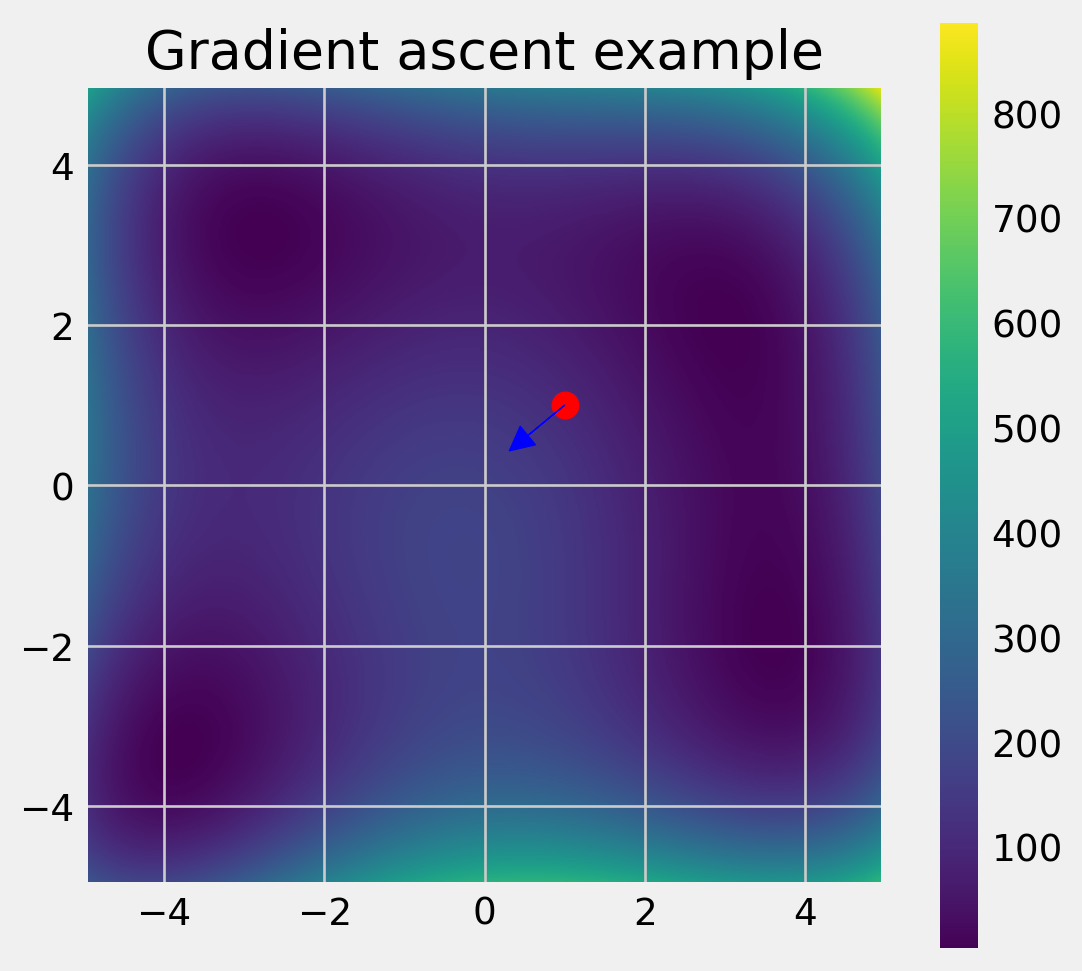
\includegraphics{pg_files/figure-pdf/cell-4-output-1.pdf}

For differentiable functions, this can be thought of as the vector of
partial derivatives,

\[
\nabla y(x, z) = \begin{pmatrix}
\frac{\partial y}{\partial x} \\
\frac{\partial y}{\partial z}
\end{pmatrix}.
\]

To calculate the \emph{slope} (aka ``directional derivative'') of the
mountain in a given direction \((\Delta x, \Delta z)\), you take the dot
product of the difference vector with the gradient. This means that the
direction with the highest slope is exactly the gradient itself, so we
can describe the gradient ascent algorithm as follows:

\begin{definition}[Gradient
ascent]\protect\hypertarget{def-gradient-ascent}{}\label{def-gradient-ascent}

\[
\begin{pmatrix}
x^{k+1} \\ z^{k+1}
\end{pmatrix}
= 
\begin{pmatrix}
x^{k} \\ z^{k}
\end{pmatrix}
+
\eta \nabla y(x^{k}, z^{k})
\]

\end{definition}

where \(k\) denotes the iteration of the algorithm and \(\eta > 0\) is a
``step size'' hyperparameter that controls the size of the steps we
take. (Note that we could also vary the step size across iterations,
that is, \(\eta^0, \dots, \eta^K\).)

The case of a two-dimensional input is easy to visualize. But this idea
can be straightforwardly extended to higher-dimensional inputs.

From now on, we'll use \(J\) to denote the function we're trying to
maximize, and \(\theta\) to denote the parameters being optimized over.
(In the above example,
\(\theta = \begin{pmatrix} x & z \end{pmatrix}^\top\)).

Notice that our parameters will stop changing once
\(\nabla J(\theta) = 0.\) Once we reach this \textbf{stationary point,}
our current parameters are `locally optimal' in some sense; it's
impossible to increase the function by moving in any direction. If \(J\)
is \emph{convex}, then the only point where this happens is at the
\emph{global optimum.} Otherwise, if \(J\) is nonconvex, the best we can
hope for is a \emph{local optimum.}

\subsection{Computing derivatives}\label{computing-derivatives}

How does a computer compute the gradient of a function?

One way is \emph{symbolic differentiation,} which is similar to the way
you might compute it by hand: the computer applies a list of rules to
transform the \emph{symbols} involved. Python's \texttt{sympy} package
supports symbolic differentiation. However, functions implemented in
code may not always have a straightforward symbolic representation.

Another way is \emph{numerical differentiation,} which is based on the
limit definition of a (directional) derivative:

\[
\nabla_{\boldsymbol{u}} J(\boldsymbol{x}) = \lim_{\varepsilon \to 0}
\frac{J(\boldsymbol{x} + \varepsilon \boldsymbol{u}) - J(\boldsymbol{x})}{\varepsilon}
\]

Then, we can substitute a small value of \(\varepsilon\) on the r.h.s.
to approximate the directional derivative. How small, though? If we need
an accurate estimate, we may need such a small value of \(\varepsilon\)
that typical computers will run into rounding errors. Also, to compute
the full gradient, we would need to compute the r.h.s. once for each
input dimension. This is an issue if computing \(J\) is expensive.

\textbf{Automatic differentiation} achieves the best of both worlds.
Like symbolic differentiation, we manually implement the derivative
rules for a few basic operations. However, instead of executing these on
the \emph{symbols}, we execute them on the \emph{values} when the
function gets called, like in numerical differentiation. This allows us
to differentiate through programming constructs such as branches or
loops, and doesn't involve any arbitrarily small values. Baydin et al.
(2018) provides an accessible survey of automatic differentiation.

\subsection{Stochastic gradient
ascent}\label{stochastic-gradient-ascent}

In real applications, computing the gradient of the target function is
not so simple. As an example from supervised learning, \(J(\theta)\)
might be the sum of squared prediction errors across an entire training
dataset. However, if our dataset is very large, it might not fit into
our computer's memory! Typically in these cases, we compute some
\emph{estimate} of the gradient at each step, and walk in that direction
instead. This is called \textbf{stochastic} gradient ascent. In the SL
example above, we might randomly choose a \emph{minibatch} of samples
and use them to estimate the true prediction error. (This approach is
known as \textbf{\emph{minibatch} SGD}.)

\begin{Shaded}
\begin{Highlighting}[]
\KeywordTok{def}\NormalTok{ sgd(}
\NormalTok{    theta\_init: Float[Array, }\StringTok{" D"}\NormalTok{],}
\NormalTok{    estimate\_gradient: Callable[[Float[Array, }\StringTok{" D"}\NormalTok{]], Float[Array, }\StringTok{" D"}\NormalTok{]],}
\NormalTok{    eta: }\BuiltInTok{float}\NormalTok{,}
\NormalTok{    n\_steps: }\BuiltInTok{int}\NormalTok{,}
\NormalTok{):}
    \CommentTok{\# Perform \textasciigrave{}n\_steps\textasciigrave{} steps of SGD.}

    \CommentTok{\# \textasciigrave{}estimate\_gradient\textasciigrave{} eats the current parameters and returns an estimate of the objective function\textquotesingle{}s gradient at those parameters.}
\NormalTok{    theta }\OperatorTok{=}\NormalTok{ theta\_init}
    \ControlFlowTok{for}\NormalTok{ step }\KeywordTok{in} \BuiltInTok{range}\NormalTok{(n\_steps):}
\NormalTok{        theta }\OperatorTok{+=}\NormalTok{ eta }\OperatorTok{*}\NormalTok{ estimate\_gradient(theta)}
    \ControlFlowTok{return}\NormalTok{ theta}

\NormalTok{latex(sgd)}
\end{Highlighting}
\end{Shaded}

$ \begin{array}{l} \mathbf{function} \ \mathrm{sgd}(\mathrm{theta\_init}, \mathrm{estimate\_gradient}, \eta, \mathrm{n\_steps}) \\ \hspace{1em} \theta \gets \mathrm{theta\_init} \\ \hspace{1em} \mathbf{for} \ \mathrm{step} \in \mathrm{range} \mathopen{}\left( \mathrm{n\_steps} \mathclose{}\right) \ \mathbf{do} \\ \hspace{2em} \theta \gets \theta + \eta \cdot \mathrm{estimate\_gradient} \mathopen{}\left( \theta \mathclose{}\right) \\ \hspace{1em} \mathbf{end \ for} \\ \hspace{1em} \mathbf{return} \ \theta \\ \mathbf{end \ function} \end{array} $

What makes one gradient estimator better than another? Ideally, we want
this estimator to be \textbf{unbiased;} that is, on average, it matches
a single true gradient step:

\[
\mathbb{E}[\tilde \nabla J(\theta)] = \nabla J(\theta).
\]

We also want the \emph{variance} of the estimator to be low so that its
performance doesn't change drastically at each step.

We can actually show that, for many ``nice'' functions, in a finite
number of steps, SGD will find a \(\theta\) that is ``close'' to a
stationary point. In another perspective, for such functions, the local
``landscape'' of \(J\) around \(\theta\) becomes flatter and flatter the
longer we run SGD.

:::\{note\} SGD convergence More formally, suppose we run SGD for \(K\)
steps, using an unbiased gradient estimator. Let the step size
\(\eta^k\) scale as \(O(1/\sqrt{k}).\) Then if \(J\) is bounded and
\(\beta\)-smooth (see below), and the \emph{norm} of the gradient
estimator has a bounded second moment \(\sigma^2,\)

\[\|\nabla J(\theta^K)\|^2 \le O \left( M \beta \sigma^2 / K\right).\]

We call a function \(\beta\)-smooth if its gradient is Lipschitz
continuous with constant \(\beta\):

\[\|\nabla J(\theta) - \nabla J(\theta')\| \le \beta \|\theta - \theta'\|.\]
:::

We'll now see a concrete application of gradient ascent in the context
of policy optimization.

\section{Policy (stochastic) gradient
ascent}\label{policy-stochastic-gradient-ascent}

Remember that in RL, the primary goal is to find the \emph{optimal
policy} that achieves the maximimum total reward, which we can express
using Definition~\ref{def-value}:

\begin{equation}\phantomsection\label{eq-objective_fn}{
\begin{aligned}
    J(\pi) := \mathbb{E}_{s_0 \sim \mu_0} V^{\pi} (s_0) = & \mathbb{E}_{\tau \sim \rho^\pi} \sum_{h=0}^{H-1} r(s_h, a_h)
\end{aligned}
}\end{equation}

where \(\rho^\pi\) is the distribution over trajectories induced by
\(\pi\) (see Definition~\ref{def-autoregressive_trajectories}).

(Note that we'll continue to work in the \emph{undiscounted,
finite-horizon case.} Analogous results hold for the \emph{discounted,
infinite-horizon setup.})

As shown by the notation, this is exactly the function \(J\) that we
want to maximize using gradient ascent. What variables are we optimizing
over in this problem? Well, the objective function \(J\) is a function
of the policy \(\pi\), but in general, \(\pi\) is a function, and
optimizing over the entire space of arbitrary input-output mappings
would be intractable. Instead, we need to describe \(\pi\) in terms of
some finite set of \emph{parameters} \(\theta\).

\subsection{Example policy
parameterizations}\label{sec-parameterizations}

What are some ways we could parameterize our policy?

\begin{example}[Tabular
representation]\protect\hypertarget{exm-tabular-repr}{}\label{exm-tabular-repr}

If both the state and action spaces are finite, perhaps we could simply
learn a preference value \(\theta_{s,a}\) for each state-action pair.
Then to turn this into a valid distribution, we perform a
\textbf{softmax} operation: we exponentiate each of them, and then
normalize to form a valid distribution.

\[\pi^\text{softmax}_\theta(a | s) = \frac{\exp(\theta_{s,a})}{\sum_{s,a'} \exp (\theta_{s,a'})}.\]

However, this doesn't make use of any structure in the states or
actions, so while this is flexible, it is also prone to overfitting.

\end{example}

\begin{example}[Linear in
features]\protect\hypertarget{exm-linear-in-features}{}\label{exm-linear-in-features}

Another approach is to map each state-action pair into some
\textbf{feature space} \(\phi(s, a) \in \mathbb{R}^p\). Then, to map a
feature vector to a probability, we take a linear combination of the
features and take a softmax:

\[\pi^\text{linear in features}_{\theta}(a|s) = \frac{\exp(\theta^\top \phi(s, a))}{\sum_{a'} \exp(\theta^\top \phi(s, a'))}.\]

Another interpretation is that \(\theta\) represents the feature vector
of the ``desired'' state-action pair, as state-action pairs whose
features align closely with \(\theta\) are given higher probability.

\end{example}

\begin{example}[Neural
policies]\protect\hypertarget{exm-neural-policy}{}\label{exm-neural-policy}

More generally, we could map states and actions to unnormalized scores
via some parameterized function
\(f_\theta : \mathcal{S} \times \mathcal{A} \to \mathbb{R},\) such as a
neural network, and choose actions according to a softmax:
\[\pi^\text{general}_\theta(a|s) = \frac{\exp(f_{\theta}(s,a))}{\sum_{a'} \exp(f_{\theta}(s,a'))}.\]

\end{example}

\begin{example}[Diagonal Gaussian policies for continuous action
spaces]\protect\hypertarget{exm-gaussian-policy}{}\label{exm-gaussian-policy}

Consider a continuous \(n\)-dimensional action space
\(\mathcal{A} = \mathbb{R}^n\). Then for a stochastic policy, we could
use a function to predict the \emph{mean} action and then add some
random noise about it. For example, we could use a neural network to
predict the mean action \(\mu_\theta(s)\) and then add some noise
\(\epsilon \sim \mathcal{N}(0, \sigma^2 I)\) to it:

\[\pi_\theta(a|s) = \mathcal{N}(\mu_\theta(s), \sigma^2 I).\]

\end{example}

Now that we have seen some examples of parameterized policies, we will
write the total reward in terms of the parameters, overloading notation
and letting \(\rho_\theta := \rho^{\pi_\theta}\):

\[J(\theta) = \mathbb{E}_{\tau \sim \rho_\theta} R(\tau)\]

where \(R(\tau) = \sum_{h=0}^{H-1} r(s_h, a_h)\) denotes the total
reward in the trajectory.

Now how do we maximize this function (the expected total reward) over
the parameters? One simple idea would be to directly apply gradient
ascent:

\[
\theta^{k+1} = \theta^k + \eta \nabla J(\theta^k).
\]

In order to apply this technique, we need to be able to evaluate the
gradient \(\nabla J(\theta).\) But \(J(\theta)\) is very difficult, or
even intractable, to compute exactly, since it involves taking an
expectation over all possible trajectories \(\tau.\) Can we rewrite it
in a form that's more convenient to implement?

\subsection{Importance Sampling}\label{sec-importance_sampling}

There is a general trick called \textbf{importance sampling} for
evaluating difficult expectations. Suppose we want to estimate
\(\mathbb{E}_{x \sim p}[f(x)]\) where \(p\) is hard or expensive to
sample from, but easy to evaluate the likelihood \(p(x)\) of. Suppose
that we \emph{can} easily sample from a different distribution \(q\).
Since an expectation is just a weighted average, we can sample \(x\)
from \(q\), compute \(f(x)\), and then reweight the results: if \(x\) is
very likely under \(p\) but unlikely under \(q\), we should boost its
weighting, and if it is common under \(q\) but uncommon under \(p\), we
should lower its weighting. The reweighting factor is exactly the
\textbf{likelihood ratio} between the target distribution \(p\) and the
sampling distribution \(q\):

\[
\mathbb{E}_{x \sim p}[f(x)] = \sum_{x \in \mathcal{X}} f(x) p(x) = \sum_{x \in \mathcal{X}} f(x) \frac{p(x)}{q(x)} q(x) = \mathbb{E}_{x \sim q} \left[ \frac{p(x)}{q(x)} f(x) \right].
\]

Doesn't this seem too good to be true? If there were no drawbacks, we
could use this to estimate \emph{any} expectation of any function on any
arbitrary distribution! The drawback is that the variance may be very
large due to the likelihood ratio term. If there are values of \(x\)
that are very rare in the sampling distribution \(q\), but common under
\(p\), then the likelihood ratio \(p(x)/q(x)\) will cause the variance
to blow up.

\section{The REINFORCE policy
gradient}\label{the-reinforce-policy-gradient}

Returning to RL, suppose there is some trajectory distribution
\(\rho(\tau)\) that is \textbf{easy to sample from,} such as a database
of existing trajectories. We can then rewrite \(\nabla J(\theta)\),
a.k.a. the \emph{policy gradient}, as follows. All gradients are being
taken with respect to \(\theta\).

\[
\begin{aligned}
    \nabla J(\theta) & = \nabla \mathbb{E}_{\tau \sim \rho_\theta} [ R(\tau) ]                                                                                         \\
                     & = \nabla \mathbb{E}_{\tau \sim \rho} \left[ \frac{\rho_\theta(\tau)}{\rho(\tau)} R(\tau) \right] &  & \text{likelihood ratio trick}             \\
                     & = \mathbb{E}_{\tau \sim \rho} \left[ \frac{\nabla \rho_\theta(\tau)}{\rho(\tau)} R(\tau) \right] &  & \text{switching gradient and expectation}
\end{aligned}
\]

Note that for \(\rho = \rho_\theta\), the inside term becomes

\[
\nabla J(\theta) = \mathbb{E}_{\tau \sim \rho_\theta} [ \nabla \log \rho_\theta(\tau) \cdot R(\tau)].
\]

(The order of operations is \(\nabla (\log \rho_\theta)(\tau)\).)

Recall that when the state transitions are Markov (i.e.~\(s_{t}\) only
depends on \(s_{t-1}, a_{t-1}\)) and the policy is time-homogeneous
(i.e.~\(a_h\sim \pi_\theta (s_h)\)), we can write out the
\emph{likelihood of a trajectory} under the policy \(\pi_\theta\)
autoregressively, as in
Definition~\ref{def-autoregressive_trajectories}. Taking the log of the
trajectory likelihood turns it into a sum of terms:

\[
\log \rho_\theta(\tau) = \log \mu(s_0) + \sum_{h=0}^{H-1} \log \pi_\theta(a_h\mid s_h) + \log P(s_{h+1} \mid s_h, a_h)
\]

When we take the gradient with respect to the parameters \(\theta\),
only the \(\pi_\theta(a_h| s_h)\) terms depend on \(\theta\). This gives
the following expression for the policy gradient, known as the
``REINFORCE'' policy gradient Williams (1992):

\begin{equation}\phantomsection\label{eq-reinforce_pg}{
\begin{aligned}
    \nabla J(\theta) = \mathbb{E}_{\tau \sim \rho_\theta} \left[ \sum_{h=0}^{H-1} \nabla_\theta \log \pi_{\theta}(a_h| s_h) R(\tau) \right]
\end{aligned}
}\end{equation}

This expression allows us to estimate the gradient by sampling a few
sample trajectories from \(\pi_\theta,\) calculating the likelihoods of
the chosen actions, and substituting these into the expression inside
the brackets of Equation~\ref{eq-reinforce_pg}. Then we can update the
parameters \(\theta\) in this direction to perform stochastic gradient
ascent.

The rest of this chapter investigates ways to \emph{reduce the variance}
of this estimator by subtracting off certain correlated quantities.

\begin{lemma}[Intuition behind
REINFORCE]\protect\hypertarget{lem-intuitive-remark}{}\label{lem-intuitive-remark}

Intuitively speaking, we want to update the policy parameters to
maximize the probability of taking \emph{optimal actions}. That is,
suppose we are in state \(s\), and \(a^\star\) is an optimal action to
take. Then we want to solve
\(\theta = \arg\max_{\theta'} \pi_{\theta'}(a^\star \mid s)\), which
would lead to the gradient ascent expression

\[
\theta \gets \theta + \nabla \pi_{\theta}(a^\star \mid s).
\]

However, we don't know the optimal action \(a^\star\) in practice. So
instead, we must try many actions, and \emph{increase} the probability
of the ``good'' ones and \emph{decrease} the probability of the ``bad''
ones. Suppose \(A(s, a)\) is a measure of how good action \(a\) is in
state \(s\). Then we could write

\[
\theta \gets \theta + \sum_a \pi_{\theta}(a \mid s) A(s, a) \nabla \pi_{\theta}(a \mid s).
\]

But this has an issue: the size of each step doesn't just depend on how
good it is, but also how \emph{often} the policy takes it already. This
could lead to a positive feedback loop where likely actions become more
and more likely, without respect to the quality of the action. So we
divide by the likelihood to cancel out this factor:

\[
\theta \gets \theta + \sum_a \pi_{\theta}(a \mid s) A(s, a) \frac{\nabla \pi_{\theta}(a \mid s)}{\pi_{\theta}(a \mid s)}.
\]

But once we simplify, and sum across timesteps, this becomes
\emph{almost} exactly the gradient written above!

\[
\theta \gets \theta + \mathbb{E}_{a \sim \pi_{\theta}(\cdot \mid s)} [\sum_{h=0}^{H-1} A(s_h, a_h) \nabla \log \pi_{\theta}(a_h\mid s_h) ].
\]

We will see later on what \(A\) concretely corresponds to.

\end{lemma}

\begin{Shaded}
\begin{Highlighting}[]
\AttributeTok{@latex}
\KeywordTok{def}\NormalTok{ estimate\_gradient\_reinforce\_pseudocode(env: gym.Env, pi, theta: Float[Array, }\StringTok{" D"}\NormalTok{]):}
\NormalTok{    tau }\OperatorTok{=}\NormalTok{ sample\_trajectory(env, pi(theta))}
\NormalTok{    nabla\_hat }\OperatorTok{=}\NormalTok{ jnp.zeros\_like(theta)}
\NormalTok{    total\_reward }\OperatorTok{=} \BuiltInTok{sum}\NormalTok{(r }\ControlFlowTok{for}\NormalTok{ \_s, \_a, r }\KeywordTok{in}\NormalTok{ tau)}
    \ControlFlowTok{for}\NormalTok{ s, a, r }\KeywordTok{in}\NormalTok{ tau:}
        \KeywordTok{def}\NormalTok{ policy\_log\_likelihood(theta: Float[Array, }\StringTok{" D"}\NormalTok{]) }\OperatorTok{{-}\textgreater{}} \BuiltInTok{float}\NormalTok{:}
            \ControlFlowTok{return}\NormalTok{ log(pi(theta)(s, a))}
\NormalTok{        nabla\_hat }\OperatorTok{+=}\NormalTok{ jax.grad(policy\_log\_likelihood)(theta) }\OperatorTok{*}\NormalTok{ total\_reward}
    \ControlFlowTok{return}\NormalTok{ nabla\_hat}

\NormalTok{estimate\_gradient\_reinforce\_pseudocode}
\end{Highlighting}
\end{Shaded}

$ \begin{array}{l} \mathbf{function} \ \mathrm{estimate\_gradient\_reinforce\_pseudocode}(\mathrm{env}, \pi, \theta) \\ \hspace{1em} \tau \gets \mathrm{sample\_trajectory} \mathopen{}\left( \mathrm{env}, \pi \mathopen{}\left( \theta \mathclose{}\right) \mathclose{}\right) \\ \hspace{1em} \mathrm{nabla\_hat} \gets \mathrm{jnp}.\mathrm{zeros\_like} \mathopen{}\left( \theta \mathclose{}\right) \\ \hspace{1em} \mathrm{total\_reward} \gets \sum_{\mathopen{}\left( \mathrm{\_s}, \mathrm{\_a}, r \mathclose{}\right) \in \tau}^{} \mathopen{}\left({r}\mathclose{}\right) \\ \hspace{1em} \mathbf{for} \ \mathopen{}\left( s, a, r \mathclose{}\right) \in \tau \ \mathbf{do} \\ \begin{array}{l} \hspace{2em} \mathbf{function} \ \mathrm{policy\_log\_likelihood}(\theta) \\ \hspace{3em} \mathbf{return} \ \log \pi \mathopen{}\left( \theta \mathclose{}\right) \mathopen{}\left( s, a \mathclose{}\right) \\ \hspace{2em} \mathbf{end \ function} \end{array} \\ \hspace{2em} \mathrm{nabla\_hat} \gets \mathrm{nabla\_hat} + \mathrm{jax}.\mathrm{grad} \mathopen{}\left( \mathrm{policy\_log\_likelihood} \mathclose{}\right) \mathopen{}\left( \theta \mathclose{}\right) \cdot \mathrm{total\_reward} \\ \hspace{1em} \mathbf{end \ for} \\ \hspace{1em} \mathbf{return} \ \mathrm{nabla\_hat} \\ \mathbf{end \ function} \end{array} $

For some intuition into how this method works, recall that we update our
parameters according to

\[
\begin{aligned}
    \theta_{t+1} &= \theta_t + \eta \nabla J(\theta_t) \\
    &= \theta_t + \eta \mathbb{E}_{\tau \sim \rho_{\theta_t}} [\nabla \log \rho_{\theta_t}(\tau) \cdot R(\tau)].
\end{aligned}
\]

Consider the ``good'' trajectories where \(R(\tau)\) is large. Then
\(\theta\) gets updated so that these trajectories become more likely.
To see why, recall that \(\rho_{\theta}(\tau)\) is the likelihood of the
trajectory \(\tau\) under the policy \(\pi_\theta,\) so the gradient
points in the direction that makes \(\tau\) more likely.

\section{Baselines and advantages}\label{baselines-and-advantages}

A central idea from supervised learning is the \textbf{bias-variance
decomposition}, which shows that the mean squared error of an estimator
is the sum of its squared bias and its variance. The REINFORCE gradient
estimator Equation~\ref{eq-reinforce_pg} is already \emph{unbiased,}
meaning that its expectation over trajectories is the true policy
gradient. Can we find ways to reduce its \emph{variance} as well?

As a first step, consider that the action taken at step \(t\) does not
affect the reward from previous timesteps, since they're already in the
past. You can also show rigorously that this is the case, and that we
only need to consider the present and future rewards to calculate the
policy gradient:

\[
\nabla J(\theta) = \mathbb{E}_{\tau \sim \rho_\theta} \left[ \sum_{h=0}^{H-1} \nabla_\theta \log \pi_{\theta}(a_h| s_h) \sum_{h' = h}^{H-1} r(s_{h'}, a_{h'}) \right]
\]

Furthermore, by a conditioning argument, we can replace the inner sum
over remaining rewards with the policy's Q-function, evaluated at the
current state:

\begin{equation}\phantomsection\label{eq-pg_with_q}{
\nabla J(\theta) = \mathbb{E}_{\tau \sim \rho_\theta} \left[ \sum_{h=0}^{H-1} \nabla_\theta \log \pi_{\theta}(a_h| s_h) Q^{\pi_\theta}(s_{h}, a_{h}) \right]
}\end{equation}

\textbf{Exercise:} Prove that this is equivalent to the previous
definitions. What modification to the expression must be made for the
discounted, infinite-horizon setting?

We can further reduce variance by subtracting a \textbf{baseline
function} \(b_h: \mathcal{S} \to \mathbb{R}\) at each timestep \(h\).
This modifies the policy gradient as follows:

\begin{equation}\phantomsection\label{eq-pg_baseline}{
\nabla J(\theta) = \mathbb{E}_{\tau \sim \rho_\theta} \left[
    \sum_{h=0}^{H-1} \nabla \log \pi_\theta (a_h| s_h) \left(
    Q^{\pi_\theta}(s_h, a_h)
    - b_h(s_h)
    \right)
    \right].
}\end{equation}

(Again, you should try to prove that this equality still holds.) For
example, we might want \(b_h\) to estimate the average reward-to-go at a
given timestep:

\[b_h^\theta = \mathbb{E}_{\tau \sim \rho_\theta} R_h(\tau).\]

As a better baseline, we could instead choose the \emph{value function.}
Note that the random variable \(Q^\pi_h(s, a) - V^\pi_h(s),\) where the
randomness is taken over the actions, is centered around zero. (Recall
\(V^\pi_h(s) = \mathbb{E}_{a \sim \pi} Q^\pi_h(s, a).\)) This quantity
matches the intuition given in Lemma~\ref{lem-intuitive-remark}: it is
\emph{positive} for actions that are better than average (in state
\(s\)), and \emph{negative} for actions that are worse than average. In
fact, this quantity has a particular name: the \textbf{advantage
function.}

\begin{definition}[Advantage
function]\protect\hypertarget{def-advantage}{}\label{def-advantage}

\[
A^\pi_h(s, a) = Q^\pi_h(s, a) - V^\pi_h(s)
\]

\end{definition}

This measures how much better this action does than the average for that
policy. (Note that for an optimal policy \(\pi^\star,\) the advantage of
a given state-action pair is always zero or negative.)

We can now express the policy gradient as follows. Note that the
advantage function effectively replaces the \(Q\)-function from
Equation~\ref{eq-pg_with_q}:

\begin{equation}\phantomsection\label{eq-pg_advantage}{
\nabla J(\theta) = \mathbb{E}_{\tau \sim \rho_\theta} \left[
        \sum_{h=0}^{H-1} \nabla \log \pi_\theta(a_h| s_h) A^{\pi_\theta}_h(s_h, a_h)
\right].
}\end{equation}

\begin{example}[Policy gradient for the linear-in-features
parameterization]\protect\hypertarget{exm-linear-policy-grad}{}\label{exm-linear-policy-grad}

The gradient-log-likelihood for the linear-in-features parameterization
Example~\ref{exm-linear-in-features} is also quite elegant:

\[
\begin{aligned}
        \nabla \log \pi_\theta(a|s) &= \nabla \left( \theta^\top \phi(s, a) - \log \left( \sum_{a'} \exp(\theta^\top \phi(s, a')) \right) \right) \\
        &= \phi(s, a) - \mathbb{E}_{a' \sim \pi_\theta(s)} \phi(s, a')
\end{aligned}
\]

Plugging this into our policy gradient expression, we get

\[\begin{aligned}
    \nabla J(\theta) & = \mathbb{E}_{\tau \sim \rho_\theta} \left[
    \sum_{t=0}^{T-1} \nabla \log \pi_\theta(a_h| s_h) A_h^{\pi_\theta}
    \right]                                                                                                                    \\
                     & = \mathbb{E}_{\tau \sim \rho_\theta} \left[
    \sum_{t=0}^{T-1} \left( \phi(s_h, a_h) - \mathbb{E}_{a' \sim \pi(s_h)} \phi(s_h, a') \right) A_h^{\pi_\theta}(s_h, a_h)
    \right]                                                                                                                    \\
                     & = \mathbb{E}_{\tau \sim \rho_\theta} \left[ \sum_{t=0}^{T-1} \phi(s_h, a_h) A_h^{\pi_\theta} (s_h, a_h) \right]
\end{aligned}
\]

Why can we drop the \(\mathbb{E}\phi(s_h, a')\) term? By linearity of
expectation, consider the dropped term at a single timestep:
\(\mathbb{E}_{\tau \sim \rho_\theta} \left[ \left( \mathbb{E}_{a' \sim \pi(s_h)} \phi(s, a') \right) A_h^{\pi_\theta}(s_h, a_h) \right].\)
By Adam's Law, we can wrap the advantage term in a conditional
expectation on the state \(s_h.\) Then we already know that
\(\mathbb{E}_{a \sim \pi(s)} A_h^{\pi}(s, a) = 0,\) and so this entire
term vanishes.

\end{example}

Note that to avoid correlations between the gradient estimator and the
value estimator (i.e.~baseline), we must estimate them with
independently sampled trajectories:

\begin{Shaded}
\begin{Highlighting}[]
\KeywordTok{def}\NormalTok{ pg\_with\_learned\_baseline(env: gym.Env, pi, eta: }\BuiltInTok{float}\NormalTok{, theta\_init, K: }\BuiltInTok{int}\NormalTok{, N: }\BuiltInTok{int}\NormalTok{) }\OperatorTok{{-}\textgreater{}}\NormalTok{ Float[Array, }\StringTok{" D"}\NormalTok{]:}
\NormalTok{    theta }\OperatorTok{=}\NormalTok{ theta\_init}
    \ControlFlowTok{for}\NormalTok{ k }\KeywordTok{in} \BuiltInTok{range}\NormalTok{(K):}
\NormalTok{        trajectories }\OperatorTok{=}\NormalTok{ sample\_trajectories(env, pi(theta), N)}
\NormalTok{        V\_hat }\OperatorTok{=}\NormalTok{ fit\_value(trajectories)}
\NormalTok{        tau }\OperatorTok{=}\NormalTok{ sample\_trajectories(env, pi(theta), }\DecValTok{1}\NormalTok{)}
\NormalTok{        nabla\_hat }\OperatorTok{=}\NormalTok{ jnp.zeros\_like(theta)  }\CommentTok{\# gradient estimator}

        \ControlFlowTok{for}\NormalTok{ h, (s, a) }\KeywordTok{in} \BuiltInTok{enumerate}\NormalTok{(tau):}
            \KeywordTok{def}\NormalTok{ log\_likelihood(theta\_opt):}
                \ControlFlowTok{return}\NormalTok{ jnp.log(pi(theta\_opt)(s, a))}
\NormalTok{            nabla\_hat }\OperatorTok{=}\NormalTok{ nabla\_hat }\OperatorTok{+}\NormalTok{ jax.grad(log\_likelihood)(theta) }\OperatorTok{*}\NormalTok{ (return\_to\_go(tau, h) }\OperatorTok{{-}}\NormalTok{ V\_hat(s))}
        
\NormalTok{        theta }\OperatorTok{=}\NormalTok{ theta }\OperatorTok{+}\NormalTok{ eta }\OperatorTok{*}\NormalTok{ nabla\_hat}
    \ControlFlowTok{return}\NormalTok{ theta}

\NormalTok{latex(pg\_with\_learned\_baseline)}
\end{Highlighting}
\end{Shaded}

$ \begin{array}{l} \mathbf{function} \ \mathrm{pg\_with\_learned\_baseline}(\mathrm{env}, \pi, \eta, \mathrm{theta\_init}, K, N) \\ \hspace{1em} \theta \gets \mathrm{theta\_init} \\ \hspace{1em} \mathbf{for} \ k \in \mathrm{range} \mathopen{}\left( K \mathclose{}\right) \ \mathbf{do} \\ \hspace{2em} \mathrm{trajectories} \gets \mathrm{sample\_trajectories} \mathopen{}\left( \mathrm{env}, \pi \mathopen{}\left( \theta \mathclose{}\right), N \mathclose{}\right) \\ \hspace{2em} \mathrm{V\_hat} \gets \mathrm{fit\_value} \mathopen{}\left( \mathrm{trajectories} \mathclose{}\right) \\ \hspace{2em} \tau \gets \mathrm{sample\_trajectories} \mathopen{}\left( \mathrm{env}, \pi \mathopen{}\left( \theta \mathclose{}\right), 1 \mathclose{}\right) \\ \hspace{2em} \mathrm{nabla\_hat} \gets \mathrm{jnp}.\mathrm{zeros\_like} \mathopen{}\left( \theta \mathclose{}\right) \\ \hspace{2em} \mathbf{for} \ \mathopen{}\left( h, \mathopen{}\left( s, a \mathclose{}\right) \mathclose{}\right) \in \mathrm{enumerate} \mathopen{}\left( \tau \mathclose{}\right) \ \mathbf{do} \\ \begin{array}{l} \hspace{3em} \mathbf{function} \ \mathrm{log\_likelihood}(\mathrm{theta\_opt}) \\ \hspace{4em} \mathbf{return} \ \log \pi \mathopen{}\left( \mathrm{theta\_opt} \mathclose{}\right) \mathopen{}\left( s, a \mathclose{}\right) \\ \hspace{3em} \mathbf{end \ function} \end{array} \\ \hspace{3em} \mathrm{nabla\_hat} \gets \mathrm{nabla\_hat} + \mathrm{jax}.\mathrm{grad} \mathopen{}\left( \mathrm{log\_likelihood} \mathclose{}\right) \mathopen{}\left( \theta \mathclose{}\right) \cdot \mathopen{}\left( \mathrm{return\_to\_go} \mathopen{}\left( \tau, h \mathclose{}\right) - \mathrm{V\_hat} \mathopen{}\left( s \mathclose{}\right) \mathclose{}\right) \\ \hspace{2em} \mathbf{end \ for} \\ \hspace{2em} \theta \gets \theta + \eta \cdot \mathrm{nabla\_hat} \\ \hspace{1em} \mathbf{end \ for} \\ \hspace{1em} \mathbf{return} \ \theta \\ \mathbf{end \ function} \end{array} $

Note that you could also generalize this by allowing the learning rate
\(\eta\) to vary across steps, or take multiple trajectories \(\tau\)
and compute the sample average of the gradient estimates.

The baseline estimation step \texttt{fit\_value} can be done using any
appropriate supervised learning algorithm. Note that the gradient
estimator will be unbiased regardless of the baseline.

\section{Comparing policy gradient algorithms to policy
iteration}\label{comparing-policy-gradient-algorithms-to-policy-iteration}

What advantages does the policy gradient algorithm have over the policy
iteration algorithms covered in Section~\ref{sec-policy_iteration}?

:::\{note\} Policy iteration recap Recall that policy iteration is an
algorithm for MDPs with unknown state transitions where we alternate
between these two steps:

\begin{itemize}
\tightlist
\item
  Estimating the \(Q\)-function (or advantage function) of the current
  policy;
\item
  Updating the policy to be greedy with respect to this approximate
  \(Q\)-function (or advantage function). :::
\end{itemize}

To analyze the difference between them, we'll make use of the
\textbf{performance difference lemma}, which provides an expression for
comparing the difference between two value functions.

\begin{theorem}[Performance difference
lemma]\protect\hypertarget{thm-pdl}{}\label{thm-pdl}

Suppose Alice is playing a game (an MDP). Bob is spectating, and can
evaluate how good an action is compared to his own strategy. (That is,
Bob can compute his \emph{advantage function}
\(A_h^{\text{Bob}}(s_h, a_h)\)). The performance difference lemma says
that Bob can now calculate exactly how much better or worse he is than
Alice as follows:

\begin{equation}\phantomsection\label{eq-pdl_eq}{
V_0^{\text{Alice}}(s) - V_0^{\text{Bob}}(s) = \mathbb{E}_{\tau \sim \rho_{\text{Alice}, s}} \left[ \sum_{h=0}^{H-1} A_h^{\text{Bob}} (s_h, a_h) \right]
}\end{equation}

where \(\rho_{\text{Alice}, s}\) denotes the distribution over
trajectories starting in state \(s\) when Alice is playing.

To see why, consider a specific step \(h\) in the trajectory. We compute
how much better actions from Bob are than the actions from Alice, on
average. But this is exactly the average Bob-advantage across actions
from Alice, as described in the PDL!

Formally, this corresponds to a nice telescoping simplification when we
expand out the definition of the advantage function. Note that

\[
\begin{aligned}
A^\pi_h(s_h, a_h) &= Q^\pi_h(s_h, a_h) - V^\pi_h(s_h) \\
&= r_h(s_h, a_h) + \mathbb{E}_{s_{h+1} \sim P(s_h, a_h)} [V^\pi_{h+1}(s_{h+1})] - V^\pi_h(s_h)
\end{aligned}
\]

so expanding out the r.h.s. expression of Equation~\ref{eq-pdl_eq} and
grouping terms together gives

\[
\begin{aligned}
\mathbb{E}_{\tau \sim \rho_{\text{Alice}, s}} \left[ \sum_{h=0}^{H-1} A_h^{\text{Bob}} (s_h, a_h) \right] &= \mathbb{E}_{\tau \sim \rho_{\text{Alice}, s}} \left[ \left( \sum_{h=0}^{H-1} r_h(s_h, a_h) \right) + \left( V^{\text{Bob}}_1(s_1) + \cdots + V^{\text{Bob}}_H(s_H) \right) - \left( V^{\text{Bob}_0}(s_0) + \cdots + V^{\text{Bob}}_{H-1}(s_{H-1}) \right) \right] \\
&= V^{\text{Alice}}_0(s) - V^{\text{Bob}}_0(s)
\end{aligned}
\]

as desired. (Note that the ``inner'' expectation from expanding the
advantage function has the same distribution as the outer one, so
omitting it here is valid.)

\end{theorem}

The PDL gives insight into why fitted approaches such as PI don't work
as well in the ``full'' RL setting. To see why, let's consider a single
iteration of policy iteration, where policy \(\pi\) gets updated to
\(\tilde \pi\). We'll assume these policies are deterministic. Suppose
the new policy \(\tilde \pi\) chooses some action with a negative
advantage with respect to \(\pi\). That is, when acting according to
\(\pi\), taking the action from \(\tilde \pi\) would perform worse than
expected. Define \(\Delta_\infty\) to be the most negative advantage,
that is,
\(\Delta_\infty = \min_{s \in \mathcal{S}} A^{\pi}_h(s, \tilde \pi(s))\).
Plugging this into the Theorem~\ref{thm-pdl} gives

\[
\begin{aligned}
V_0^{\tilde \pi}(s) - V_0^{\pi}(s) &= \mathbb{E}_{\tau \sim \rho_{\tilde \pi, s}} \left[
\sum_{h=0}^{H-1} A_h^{\pi}(s_h, a_h)
\right] \\
&\ge H \Delta_\infty \\
V_0^{\tilde \pi}(s) &\ge V_0^{\pi}(s) - H|\Delta_\infty|.
\end{aligned}
\]

That is, for some state \(s\), the lower bound on the performance of
\(\tilde \pi\) is \emph{lower} than the performance of \(\pi\). This
doesn't state that \(\tilde \pi\) \emph{will} necessarily perform worse
than \(\pi\), only suggests that it might be possible. If these worst
case states do exist, though, PI does not avoid situations where the new
policy often visits them; It does not enforce that the trajectory
distributions \(\rho_\pi\) and \(\rho_{\tilde \pi}\) be close to each
other. In other words, the ``training distribution'' that our prediction
rule is fitted on, \(\rho_\pi\), may differ significantly from the
``evaluation distribution'' \(\rho_{\tilde \pi}\).

On the other hand, policy gradient methods \emph{do}, albeit implicitly,
encourage \(\rho_\pi\) and \(\rho_{\tilde \pi}\) to be similar. Suppose
that the mapping from policy parameters to trajectory distributions is
relatively smooth. Then, by adjusting the parameters only a small
distance, the new policy will also have a similar trajectory
distribution. But this is not very rigorous, and in practice the
parameter-to-distribution mapping may not be so smooth. Can we constrain
the distance between the resulting distributions more \emph{explicitly}?

This brings us to the next three methods: - \textbf{trust region policy
optimization} (TRPO), which explicitly constrains the difference between
the distributions before and after each step; - the \textbf{natural
policy gradient} (NPG), a first-order approximation of TRPO; -
\textbf{proximal policy optimization} (PPO), a ``soft relaxation'' of
TRPO.

\section{Trust region policy optimization}\label{sec-trpo}

We saw above that policy gradient methods are effective because they
implicitly constrain how much the policy changes at each iteration. Can
we design an algorithm that \emph{explicitly} constrains the ``step
size''? That is, we want to \emph{improve} the policy as much as
possible, measured in terms of the r.h.s. of the Theorem~\ref{thm-pdl},
while ensuring that its trajectory distribution does not change too
much:

\[
\begin{aligned}
\theta^{k+1} &\gets \arg\max_{\theta^{\text{opt}}} \mathbb{E}_{s_0, \dots, s_{H-1} \sim \pi^{k}} \left[ \sum_{h=0}^{H-1} \mathbb{E}_{a_h\sim \pi^{\theta^\text{opt}}(s_h)} A^{\pi^{k}}(s_h, a_h) \right] \\
& \text{where } \text{distance}(\rho_{\theta^{\text{opt}}}, \rho_{\theta^k}) < \delta
\end{aligned}
\]

Note that we have made a small change to the r.h.s. expression: we use
the \emph{states} sampled from the old policy, and only use the
\emph{actions} from the new policy. It would be computationally
infeasible to sample entire trajectories from \(\pi_\theta\) as we are
optimizing over \(\theta\). On the other hand, if \(\pi_\theta\) returns
a vector representing a probability distribution over actions, then
evaluating the expected advantage with respect to this distribution only
requires taking a dot product. This approximation also matches the
r.h.s. of the PDL to first order in \(\theta\). (We will elaborate more
on this later.)

How do we describe the distance between \(\rho_{\theta^{\text{opt}}}\)
and \(\rho_{\theta^k}\)? We'll use the \textbf{Kullback-Leibler
divergence (KLD)}:

\begin{definition}[Kullback-Leibler
divergence]\protect\hypertarget{def-kld}{}\label{def-kld}

For two PDFs \(p, q\),

\[\mathrm{KL}\left(p\parallel q\right) := \mathbb{E}_{x \sim p} \left[ \log \frac{p(x)}{q(x)} \right]\]

This can be interpreted in many different ways, many stemming from
information theory. One such interpretation is that
\(\mathrm{KL}\left(p\parallel q\right)\) describes my average
``surprise'' if I \emph{think} data is being generated by \(q\) but it's
actually generated by \(p\). (The \textbf{surprise} of an event with
probability \(p\) is \(- \log_2 p\).) Note that
\(\mathrm{KL}\left(p\parallel q\right) = 0\) if and only if \(p = q\).
Also note that it is generally \emph{not} symmetric.

\end{definition}

Both the objective function and the KLD constraint involve a weighted
average over the space of all trajectories. This is intractable in
general, so we need to estimate the expectation. As before, we can do
this by taking an empirical average over samples from the trajectory
distribution. This gives us the following pseudocode:

\begin{Shaded}
\begin{Highlighting}[]
\KeywordTok{def}\NormalTok{ kl\_div\_trajectories(pi, theta\_1, theta\_2, trajectories):}
    \CommentTok{\# Assume trajectories are sampled from pi(theta\_1)}
\NormalTok{    kl\_div }\OperatorTok{=} \DecValTok{0}
    \ControlFlowTok{for}\NormalTok{ tau }\KeywordTok{in}\NormalTok{ trajectories:}
        \ControlFlowTok{for}\NormalTok{ s, a, \_r }\KeywordTok{in}\NormalTok{ tau:}
\NormalTok{            kl\_div }\OperatorTok{+=}\NormalTok{ jnp.log(pi(theta\_1)(s, a)) }\OperatorTok{{-}}\NormalTok{ jnp.log(pi(theta\_2)(s, a))}
    \ControlFlowTok{return}\NormalTok{ kl\_div }\OperatorTok{/} \BuiltInTok{len}\NormalTok{(trajectories)}

\NormalTok{latex(kl\_div\_trajectories)}
\end{Highlighting}
\end{Shaded}

$ \begin{array}{l} \mathbf{function} \ \mathrm{kl\_div\_trajectories}(\pi, \mathrm{theta\_1}, \mathrm{theta\_2}, \mathrm{trajectories}) \\ \hspace{1em} \mathrm{kl\_div} \gets 0 \\ \hspace{1em} \mathbf{for} \ \tau \in \mathrm{trajectories} \ \mathbf{do} \\ \hspace{2em} \mathbf{for} \ \mathopen{}\left( s, a, \mathrm{\_r} \mathclose{}\right) \in \tau \ \mathbf{do} \\ \hspace{3em} \mathrm{kl\_div} \gets \mathrm{kl\_div} + \log \pi \mathopen{}\left( \mathrm{theta\_1} \mathclose{}\right) \mathopen{}\left( s, a \mathclose{}\right) - \log \pi \mathopen{}\left( \mathrm{theta\_2} \mathclose{}\right) \mathopen{}\left( s, a \mathclose{}\right) \\ \hspace{2em} \mathbf{end \ for} \\ \hspace{1em} \mathbf{end \ for} \\ \hspace{1em} \mathbf{return} \ \frac{\mathrm{kl\_div}}{\mathrm{len} \mathopen{}\left( \mathrm{trajectories} \mathclose{}\right)} \\ \mathbf{end \ function} \end{array} $

\begin{Shaded}
\begin{Highlighting}[]
\KeywordTok{def}\NormalTok{ trpo(env, δ, theta\_init, n\_interactions):}
\NormalTok{    theta }\OperatorTok{=}\NormalTok{ theta\_init}
    \ControlFlowTok{for}\NormalTok{ k }\KeywordTok{in} \BuiltInTok{range}\NormalTok{(K):}
\NormalTok{        trajectories }\OperatorTok{=}\NormalTok{ sample\_trajectories(env, pi(theta), n\_interactions)}
\NormalTok{        A\_hat }\OperatorTok{=}\NormalTok{ fit\_advantage(trajectories)}
        
        \KeywordTok{def}\NormalTok{ approximate\_gain(theta\_opt):}
\NormalTok{            A\_total }\OperatorTok{=} \DecValTok{0}
            \ControlFlowTok{for}\NormalTok{ tau }\KeywordTok{in}\NormalTok{ trajectories:}
                \ControlFlowTok{for}\NormalTok{ s, \_a, \_r }\KeywordTok{in}\NormalTok{ tau:}
                    \ControlFlowTok{for}\NormalTok{ a }\KeywordTok{in}\NormalTok{ env.action\_space:}
\NormalTok{                        A\_total }\OperatorTok{+=}\NormalTok{ pi(theta)(s, a) }\OperatorTok{*}\NormalTok{ A\_hat(s, a)}
            \ControlFlowTok{return}\NormalTok{ A\_total}
        
        \KeywordTok{def}\NormalTok{ constraint(theta\_opt):}
            \ControlFlowTok{return}\NormalTok{ kl\_div\_trajectories(pi, theta, theta\_opt, trajectories) }\OperatorTok{\textless{}=}\NormalTok{ δ}
        
\NormalTok{        theta }\OperatorTok{=}\NormalTok{ optimize(approximate\_gain, constraint)}

    \ControlFlowTok{return}\NormalTok{ theta}

\NormalTok{latex(trpo)}
\end{Highlighting}
\end{Shaded}

$ \begin{array}{l} \mathbf{function} \ \mathrm{trpo}(\mathrm{env}, δ, \mathrm{theta\_init}, \mathrm{n\_interactions}) \\ \hspace{1em} \theta \gets \mathrm{theta\_init} \\ \hspace{1em} \mathbf{for} \ k \in \mathrm{range} \mathopen{}\left( K \mathclose{}\right) \ \mathbf{do} \\ \hspace{2em} \mathrm{trajectories} \gets \mathrm{sample\_trajectories} \mathopen{}\left( \mathrm{env}, \pi \mathopen{}\left( \theta \mathclose{}\right), \mathrm{n\_interactions} \mathclose{}\right) \\ \hspace{2em} \mathrm{A\_hat} \gets \mathrm{fit\_advantage} \mathopen{}\left( \mathrm{trajectories} \mathclose{}\right) \\ \begin{array}{l} \hspace{2em} \mathbf{function} \ \mathrm{approximate\_gain}(\mathrm{theta\_opt}) \\ \hspace{3em} \mathrm{A\_total} \gets 0 \\ \hspace{3em} \mathbf{for} \ \tau \in \mathrm{trajectories} \ \mathbf{do} \\ \hspace{4em} \mathbf{for} \ \mathopen{}\left( s, \mathrm{\_a}, \mathrm{\_r} \mathclose{}\right) \in \tau \ \mathbf{do} \\ \hspace{5em} \mathbf{for} \ a \in \mathrm{env}.\mathrm{action\_space} \ \mathbf{do} \\ \hspace{6em} \mathrm{A\_total} \gets \mathrm{A\_total} + \pi \mathopen{}\left( \theta \mathclose{}\right) \mathopen{}\left( s, a \mathclose{}\right) \cdot \mathrm{A\_hat} \mathopen{}\left( s, a \mathclose{}\right) \\ \hspace{5em} \mathbf{end \ for} \\ \hspace{4em} \mathbf{end \ for} \\ \hspace{3em} \mathbf{end \ for} \\ \hspace{3em} \mathbf{return} \ \mathrm{A\_total} \\ \hspace{2em} \mathbf{end \ function} \end{array} \\ \begin{array}{l} \hspace{2em} \mathbf{function} \ \mathrm{constraint}(\mathrm{theta\_opt}) \\ \hspace{3em} \mathbf{return} \ \mathrm{kl\_div\_trajectories} \mathopen{}\left( \pi, \theta, \mathrm{theta\_opt}, \mathrm{trajectories} \mathclose{}\right) \le δ \\ \hspace{2em} \mathbf{end \ function} \end{array} \\ \hspace{2em} \theta \gets \mathrm{optimize} \mathopen{}\left( \mathrm{approximate\_gain}, \mathrm{constraint} \mathclose{}\right) \\ \hspace{1em} \mathbf{end \ for} \\ \hspace{1em} \mathbf{return} \ \theta \\ \mathbf{end \ function} \end{array} $

The above isn't entirely complete: we still need to solve the actual
optimization problem at each step. Unless we know additional properties
of the problem, this might be an intractable optimization. Do we need to
solve it exactly, though? Instead, if we assume that both the objective
function and the constraint are somewhat smooth in terms of the policy
parameters, we can use their \emph{Taylor expansions} to give us a
simpler optimization problem with a closed-form solution. This brings us
to the \textbf{natural policy gradient} algorithm.

\section{Natural policy gradient}\label{natural-policy-gradient}

We take a \emph{linear} (first-order) approximation to the objective
function and a \emph{quadratic} (second-order) approximation to the KL
divergence constraint about the current estimate \(\theta^k\). This
results in the optimization problem

\begin{equation}\phantomsection\label{eq-npg_optimization}{
\begin{gathered}
    \max_\theta \nabla_\theta J(\pi_{\theta^k})^\top (\theta - \theta^k) \\
    \text{where } \frac{1}{2} (\theta - \theta^k)^\top F_{\theta^k} (\theta - \theta^k) \le \delta
\end{gathered}
}\end{equation}

where \(F_{\theta^k}\) is the \textbf{Fisher information matrix} defined
below.

\begin{definition}[Fisher information
matrix]\protect\hypertarget{def-fisher_matrix}{}\label{def-fisher_matrix}

Let \(p_\theta\) denote a parameterized distribution. Its Fisher
information matrix \(F_\theta\) can be defined equivalently as:

\[
\begin{aligned}
        F_{\theta} & = \mathbb{E}_{x \sim p_\theta} \left[ (\nabla_\theta \log p_\theta(x)) (\nabla_\theta \log p_\theta(x))^\top \right] & \text{covariance matrix of the Fisher score}          \\
                   & = \mathbb{E}_{x \sim p_{\theta}} [- \nabla_\theta^2 \log p_\theta(x)]                                                & \text{average Hessian of the negative log-likelihood}
\end{aligned}
\]

Recall that the Hessian of a function describes its curvature: for a
vector \(\delta \in \Theta\), the quantity
\(\delta^\top F_\theta \delta\) describes how rapidly the negative
log-likelihood changes if we move by \(\delta\). The Fisher information
matrix is precisely the Hessian of the KL divergence (with respect to
either one of the parameters).

In particular, when \(p_\theta = \rho_{\theta}\) denotes a trajectory
distribution, we can further simplify the expression:

\begin{equation}\phantomsection\label{eq-fisher_trajectory}{
F_{\theta} = \mathbb{E}_{\tau \sim \rho_\theta} \left[ \sum_{h=0}^{H-1} (\nabla \log \pi_\theta (a_h\mid s_h)) (\nabla \log \pi_\theta(a_h\mid s_h))^\top \right]
}\end{equation}

Note that we've used the Markov property to cancel out the cross terms
corresponding to two different time steps.

\end{definition}

This is a convex optimization problem with a closed-form solution. To
see why, it helps to visualize the case where \(\theta\) is
two-dimensional: the constraint describes the inside of an ellipse, and
the objective function is linear, so we can find the extreme point on
the boundary of the ellipse. We recommend Boyd and Vandenberghe (2004)
for a comprehensive treatment of convex optimization.

More generally, for a higher-dimensional \(\theta\), we can compute the
global optima by setting the gradient of the Lagrangian to zero:

\[
\begin{aligned}
    \mathcal{L}(\theta, \alpha)                     & = \nabla J(\pi_{\theta^k})^\top (\theta - \theta^k) - \alpha \left[ \frac{1}{2} (\theta - \theta^k)^\top F_{\theta^k} (\theta - \theta^k) - \delta \right] \\
    \nabla \mathcal{L}(\theta^{k+1}, \alpha) & := 0                                                                                                                                                             \\
    \implies \nabla J(\pi_{\theta^k})        & = \alpha F_{\theta^k} (\theta^{k+1} - \theta^k)                                                                                                                   \\
    \theta^{k+1}                           & = \theta^k + \eta F_{\theta^k}^{-1} \nabla J(\pi_{\theta^k})                                                                                             \\
    \text{where } \eta                     & = \sqrt{\frac{2 \delta}{\nabla J(\pi_{\theta^k})^\top F_{\theta^k}^{-1} \nabla J(\pi_{\theta^k})}}
\end{aligned}
\]

This gives us the closed-form update. Now the only challenge is to
estimate the Fisher information matrix, since, as with the KL divergence
constraint, it is an expectation over trajectories, and computing it
exactly is therefore typically intractable.

\begin{definition}[Natural policy
gradient]\protect\hypertarget{def-npg}{}\label{def-npg}

How many trajectory samples do we need to accurately estimate the Fisher
information matrix? As a rule of thumb, the sample complexity should
scale with the dimension of the parameter space. This makes this
approach intractable in the deep learning setting where we might have a
very large number of parameters.

\end{definition}

As you can see, the NPG is the ``basic'' policy gradient algorithm we
saw above, but with the gradient transformed by the inverse Fisher
information matrix. This matrix can be understood as accounting for the
\textbf{geometry of the parameter space.} The typical gradient descent
algorithm implicitly measures distances between parameters using the
typical \emph{Euclidean distance}. Here, where the parameters map to a
\emph{distribution}, using the natural gradient update is equivalent to
optimizing over \textbf{distribution space} rather than parameter space,
where distance between distributions is measured by the
Definition~\ref{def-kld}.

\begin{example}[Natural gradient on a simple
problem]\protect\hypertarget{exm-natural_simple}{}\label{exm-natural_simple}

Let's step away from RL and consider the following optimization problem
over Bernoulli distributions \(\pi \in \Delta(\{ 0, 1 \})\):

\[
\begin{aligned}
        J(\pi) & = 100 \cdot \pi(1) + 1 \cdot \pi(0)
\end{aligned}
\]

We can think of the space of such distributions as the line between
\((0, 1)\) to \((1, 0)\) on the Cartesian plane:

:::\{image\} shared/npg\_line.png :alt: a line from (0, 1) to (1, 0)
:width: 240px :align: center

\end{example}

Clearly the optimal distribution is the constant one \(\pi(1) = 1\).
Suppose we optimize over the parameterized family
\(\pi_\theta(1) = \frac{\exp(\theta)}{1+\exp(\theta)}\). Then our
optimization algorithm should set \(\theta\) to be unboundedly large.
Then the ``vanilla'' gradient is

\[\nabla_\theta J(\pi_\theta) = \frac{99 \exp(\theta)}{(1 + \exp(\theta))^2}.\]

Note that as \(\theta \to \infty\) that the increments get closer and
closer to \(0\); the rate of increase becomes exponentially slow.

However, if we compute the Fisher information ``matrix'' (which is just
a scalar in this case), we can account for the geometry induced by the
parameterization.

\[
\begin{aligned}
        F_\theta & = \mathbb{E}_{x \sim \pi_\theta} [ (\nabla_\theta \log \pi_\theta(x))^2 ] \\
                 & = \frac{\exp(\theta)}{(1 + \exp(\theta))^2}.
\end{aligned}
\]

This gives the natural gradient update

\[
\begin{aligned}
        \theta^{k+1} & = \theta^k + \eta F_{\theta^k}^{-1} \nabla_ \theta J(\theta^k) \\
                     & = \theta^k + 99 \eta
\end{aligned}
\]

which increases at a constant rate, i.e.~improves the objective more
quickly than ``vanilla'' gradient ascent. ::::

Though the NPG now gives a closed-form optimization step, it requires
computing the inverse Fisher information matrix, which typically scales
as \(O((\dim \Theta)^3)\). This can be expensive if the parameter space
is large. Can we find an algorithm that works in \emph{linear time} with
respect to the dimension of the parameter space?

\section{Proximal policy optimization}\label{sec-ppo}

We can relax the TRPO optimization problem in a different way: Rather
than imposing a hard constraint on the KL distance, we can instead
impose a \emph{soft} constraint by incorporating it into the objective
and penalizing parameter values that drastically change the trajectory
distribution.

\[
\begin{aligned}
\theta^{k+1} &\gets \arg\max_{\theta} \mathbb{E}_{s_0, \dots, s_{H-1} \sim \rho_{\pi^{k}}} \left[ \sum_{h=0}^{H-1} \mathbb{E}_{a_h\sim \pi_{\theta}(s_h)} A^{\pi^{k}}(s_h, a_h) \right] - \lambda \mathrm{KL}\left(\rho_{\theta}\parallel\rho_{\theta^k}\right)
\end{aligned}
\]

Here \(\lambda\) is a \textbf{regularization hyperparameter} that
controls the tradeoff between the two terms. This is the objective of
the \textbf{proximal policy optimization} algorithm (Schulman et al.
(2017)).

How do we solve this optimization? Let us begin by simplifying the
\(\mathrm{KL}\left(\rho_{\pi^k}\parallel\rho_{\pi_{\theta}}\right)\)
term. Expanding gives

\[
\begin{aligned}
    \mathrm{KL}\left(\rho_{\pi^k}\parallel\rho_{\pi_{\theta}}\right) & = \mathbb{E}_{\tau \sim \rho_{\pi^k}} \left[\log \frac{\rho_{\pi^k}(\tau)}{\rho_{\pi_{\theta}}(\tau)}\right]                                                       \\
                                           & = \mathbb{E}_{\tau \sim \rho_{\pi^k}} \left[ \sum_{h=0}^{H-1} \log \frac{\pi^k(a_h\mid s_h)}{\pi_{\theta}(a_h\mid s_h)}\right] & \text{state transitions cancel} \\
                                           & = \mathbb{E}_{\tau \sim \rho_{\pi^k}} \left[ \sum_{h=0}^{H-1} \log \frac{1}{\pi_{\theta}(a_h\mid s_h)}\right] + c
\end{aligned}
\]

where \(c\) is some constant with respect to \(\theta\), and can be
ignored. This gives the objective

\[
\ell^k(\theta)
=
\mathbb{E}_{s_0, \dots, s_{H-1} \sim \rho_{\pi^{k}}} \left[ \sum_{h=0}^{H-1} \mathbb{E}_{a_h\sim \pi_{\theta}(s_h)} A^{\pi^{k}}(s_h, a_h) \right] - \lambda \mathbb{E}_{\tau \sim \rho_{\pi^k}} \left[ \sum_{h=0}^{H-1} \log \frac{1}{\pi_{\theta}(a_h\mid s_h)}\right]
\]

Once again, this takes an expectation over trajectories. But here we
cannot directly sample trajectories from \(\pi^k\), since in the first
term, the actions actually come from \(\pi_\theta\). To make this term
line up with the other expectation, we would need the actions to also
come from \(\pi^k\).

This should sound familiar: we want to estimate an expectation over one
distribution by sampling from another. We can once again use
Section~\ref{sec-importance_sampling} to rewrite the inner expectation:

\[
\mathbb{E}_{a_h\sim \pi_{\theta}(s_h)} A^{\pi^{k}}(s_h, a_h)
=
\mathbb{E}_{a_h\sim \pi^k(s_h)} \frac{\pi_\theta(a_h\mid s_h)}{\pi^k(a_h\mid s_h)} A^{\pi^{k}}(s_h, a_h)
\]

Now we can combine the expectations together to get the objective

\[
\ell^k(\theta) = \mathbb{E}_{\tau \sim \rho_{\pi^k}} \left[ \sum_{h=0}^{H-1} \left( \frac{\pi_\theta(a_h\mid s_h)}{\pi^k(a_h\mid s_h)} A^{\pi^k}(s_h, a_h) - \lambda \log \frac{1}{\pi_\theta(a_h\mid s_h)} \right) \right]
\]

Now we can estimate this function by a sample average over trajectories
from \(\pi^k\). Remember that to complete a single iteration of PPO, we
execute

\[
\theta^{k+1} \gets \arg\max_{\theta} \ell^k(\theta).
\]

If \(\ell^k\) is differentiable, we can optimize it by gradient ascent,
completing a single iteration of PPO.

\begin{Shaded}
\begin{Highlighting}[]
\ImportTok{from}\NormalTok{ typing }\ImportTok{import}\NormalTok{ TypeVar}

\NormalTok{State }\OperatorTok{=}\NormalTok{ TypeVar(}\StringTok{"State"}\NormalTok{)}
\NormalTok{Action }\OperatorTok{=}\NormalTok{ TypeVar(}\StringTok{"Action"}\NormalTok{)}

\KeywordTok{def}\NormalTok{ ppo(}
\NormalTok{    env,}
\NormalTok{    pi: Callable[[Float[Array, }\StringTok{" D"}\NormalTok{]], Callable[[State, Action], }\BuiltInTok{float}\NormalTok{]],}
\NormalTok{    λ: }\BuiltInTok{float}\NormalTok{,}
\NormalTok{    theta\_init: Float[Array, }\StringTok{" D"}\NormalTok{],}
\NormalTok{    n\_iters: }\BuiltInTok{int}\NormalTok{,}
\NormalTok{    n\_fit\_trajectories: }\BuiltInTok{int}\NormalTok{,}
\NormalTok{    n\_sample\_trajectories: }\BuiltInTok{int}\NormalTok{,}
\NormalTok{):}
\NormalTok{    theta }\OperatorTok{=}\NormalTok{ theta\_init}
    \ControlFlowTok{for}\NormalTok{ k }\KeywordTok{in} \BuiltInTok{range}\NormalTok{(n\_iters):}
\NormalTok{        fit\_trajectories }\OperatorTok{=}\NormalTok{ sample\_trajectories(env, pi(theta), n\_fit\_trajectories)}
\NormalTok{        A\_hat }\OperatorTok{=}\NormalTok{ fit(fit\_trajectories)}

\NormalTok{        sample\_trajectories }\OperatorTok{=}\NormalTok{ sample\_trajectories(env, pi(theta), n\_sample\_trajectories)}
        
        \KeywordTok{def}\NormalTok{ objective(theta\_opt):}
\NormalTok{            total\_objective }\OperatorTok{=} \DecValTok{0}
            \ControlFlowTok{for}\NormalTok{ tau }\KeywordTok{in}\NormalTok{ sample\_trajectories:}
                \ControlFlowTok{for}\NormalTok{ s, a, \_r }\KeywordTok{in}\NormalTok{ tau:}
\NormalTok{                    total\_objective }\OperatorTok{+=}\NormalTok{ pi(theta\_opt)(s, a) }\OperatorTok{/}\NormalTok{ pi(theta)(s, a) }\OperatorTok{*}\NormalTok{ A\_hat(s, a) }\OperatorTok{+}\NormalTok{ λ }\OperatorTok{*}\NormalTok{ jnp.log(pi(theta\_opt)(s, a))}
            \ControlFlowTok{return}\NormalTok{ total\_objective }\OperatorTok{/}\NormalTok{ n\_sample\_trajectories}
        
\NormalTok{        theta }\OperatorTok{=}\NormalTok{ optimize(objective, theta)}

    \ControlFlowTok{return}\NormalTok{ theta}

\NormalTok{latex(ppo)}
\end{Highlighting}
\end{Shaded}

$ \begin{array}{l} \mathbf{function} \ \mathrm{ppo}(\mathrm{env}, \pi, λ, \mathrm{theta\_init}, \mathrm{n\_iters}, \mathrm{n\_fit\_trajectories}, \mathrm{n\_sample\_trajectories}) \\ \hspace{1em} \theta \gets \mathrm{theta\_init} \\ \hspace{1em} \mathbf{for} \ k \in \mathrm{range} \mathopen{}\left( \mathrm{n\_iters} \mathclose{}\right) \ \mathbf{do} \\ \hspace{2em} \mathrm{fit\_trajectories} \gets \mathrm{sample\_trajectories} \mathopen{}\left( \mathrm{env}, \pi \mathopen{}\left( \theta \mathclose{}\right), \mathrm{n\_fit\_trajectories} \mathclose{}\right) \\ \hspace{2em} \mathrm{A\_hat} \gets \mathrm{fit} \mathopen{}\left( \mathrm{fit\_trajectories} \mathclose{}\right) \\ \hspace{2em} \mathrm{sample\_trajectories} \gets \mathrm{sample\_trajectories} \mathopen{}\left( \mathrm{env}, \pi \mathopen{}\left( \theta \mathclose{}\right), \mathrm{n\_sample\_trajectories} \mathclose{}\right) \\ \begin{array}{l} \hspace{2em} \mathbf{function} \ \mathrm{objective}(\mathrm{theta\_opt}) \\ \hspace{3em} \mathrm{total\_objective} \gets 0 \\ \hspace{3em} \mathbf{for} \ \tau \in \mathrm{sample\_trajectories} \ \mathbf{do} \\ \hspace{4em} \mathbf{for} \ \mathopen{}\left( s, a, \mathrm{\_r} \mathclose{}\right) \in \tau \ \mathbf{do} \\ \hspace{5em} \mathrm{total\_objective} \gets \mathrm{total\_objective} + \frac{\pi \mathopen{}\left( \mathrm{theta\_opt} \mathclose{}\right) \mathopen{}\left( s, a \mathclose{}\right)}{\pi \mathopen{}\left( \theta \mathclose{}\right) \mathopen{}\left( s, a \mathclose{}\right)} \mathrm{A\_hat} \mathopen{}\left( s, a \mathclose{}\right) + λ \cdot \log \pi \mathopen{}\left( \mathrm{theta\_opt} \mathclose{}\right) \mathopen{}\left( s, a \mathclose{}\right) \\ \hspace{4em} \mathbf{end \ for} \\ \hspace{3em} \mathbf{end \ for} \\ \hspace{3em} \mathbf{return} \ \frac{\mathrm{total\_objective}}{\mathrm{n\_sample\_trajectories}} \\ \hspace{2em} \mathbf{end \ function} \end{array} \\ \hspace{2em} \theta \gets \mathrm{optimize} \mathopen{}\left( \mathrm{objective}, \theta \mathclose{}\right) \\ \hspace{1em} \mathbf{end \ for} \\ \hspace{1em} \mathbf{return} \ \theta \\ \mathbf{end \ function} \end{array} $

\section{Summary}\label{summary-4}

Policy gradient methods are a powerful family of algorithms that
directly optimize the expected total reward by iteratively updating the
policy parameters. Precisely, we estimate the gradient of the expected
total reward (with respect to the parameters), and update the parameters
in that direction. But estimating the gradient is a tricky task! We saw
many ways to reduce the variance of the gradient estimator, culminating
in the advantage-based expression Equation~\ref{eq-pg_advantage}.

But updating the parameters doesn't entirely solve the problem:
Sometimes, a small step in the parameters might lead to a big step in
the policy. To avoid changing the policy too much at each step, we must
account for the curvature in the parameter space. We first did this
explicitly with Section~\ref{sec-trpo}, and then saw ways to relax the
constraint in Definition~\ref{def-npg} and Section~\ref{sec-ppo}.

These are still popular methods to this day, especially because they
efficiently integrate with \emph{deep neural networks} for representing
complex functions.

\bookmarksetup{startatroot}

\chapter{Imitation Learning}\label{sec-imitation_learning}

\begin{center}\rule{0.5\linewidth}{0.5pt}\end{center}

\begin{center}\rule{0.5\linewidth}{0.5pt}\end{center}

\providecommand{\hi}{h}
\providecommand{\hor}{H}
\providecommand{\kl}[2]{\mathrm{KL}\left(#1\parallel#2\right)}
\providecommand{\ind}[1]{\mathbf{1}\left\{#1\right\}}
\providecommand{\st}{s}
\providecommand{\act}{a}
\providecommand{\E}{\mathbb{E}}
\providecommand{\R}{\mathbb{R}}
\providecommand{\pr}{\mathbb{P}}

\section{Introduction}\label{introduction-7}

Imagine you are tasked with learning how to drive. How do, or did, you
go about it? At first, this task might seem insurmountable: there are a
vast array of controls, and the cost of making a single mistake could be
extremely high, making it hard to explore by trial and error. Luckily,
there are already people in the world who know how to drive who can get
you started. In almost every challenge we face, we ``stand on the
shoulders of giants'' and learn skills from experts who have already
mastered them.

\begin{figure}[H]

{\centering 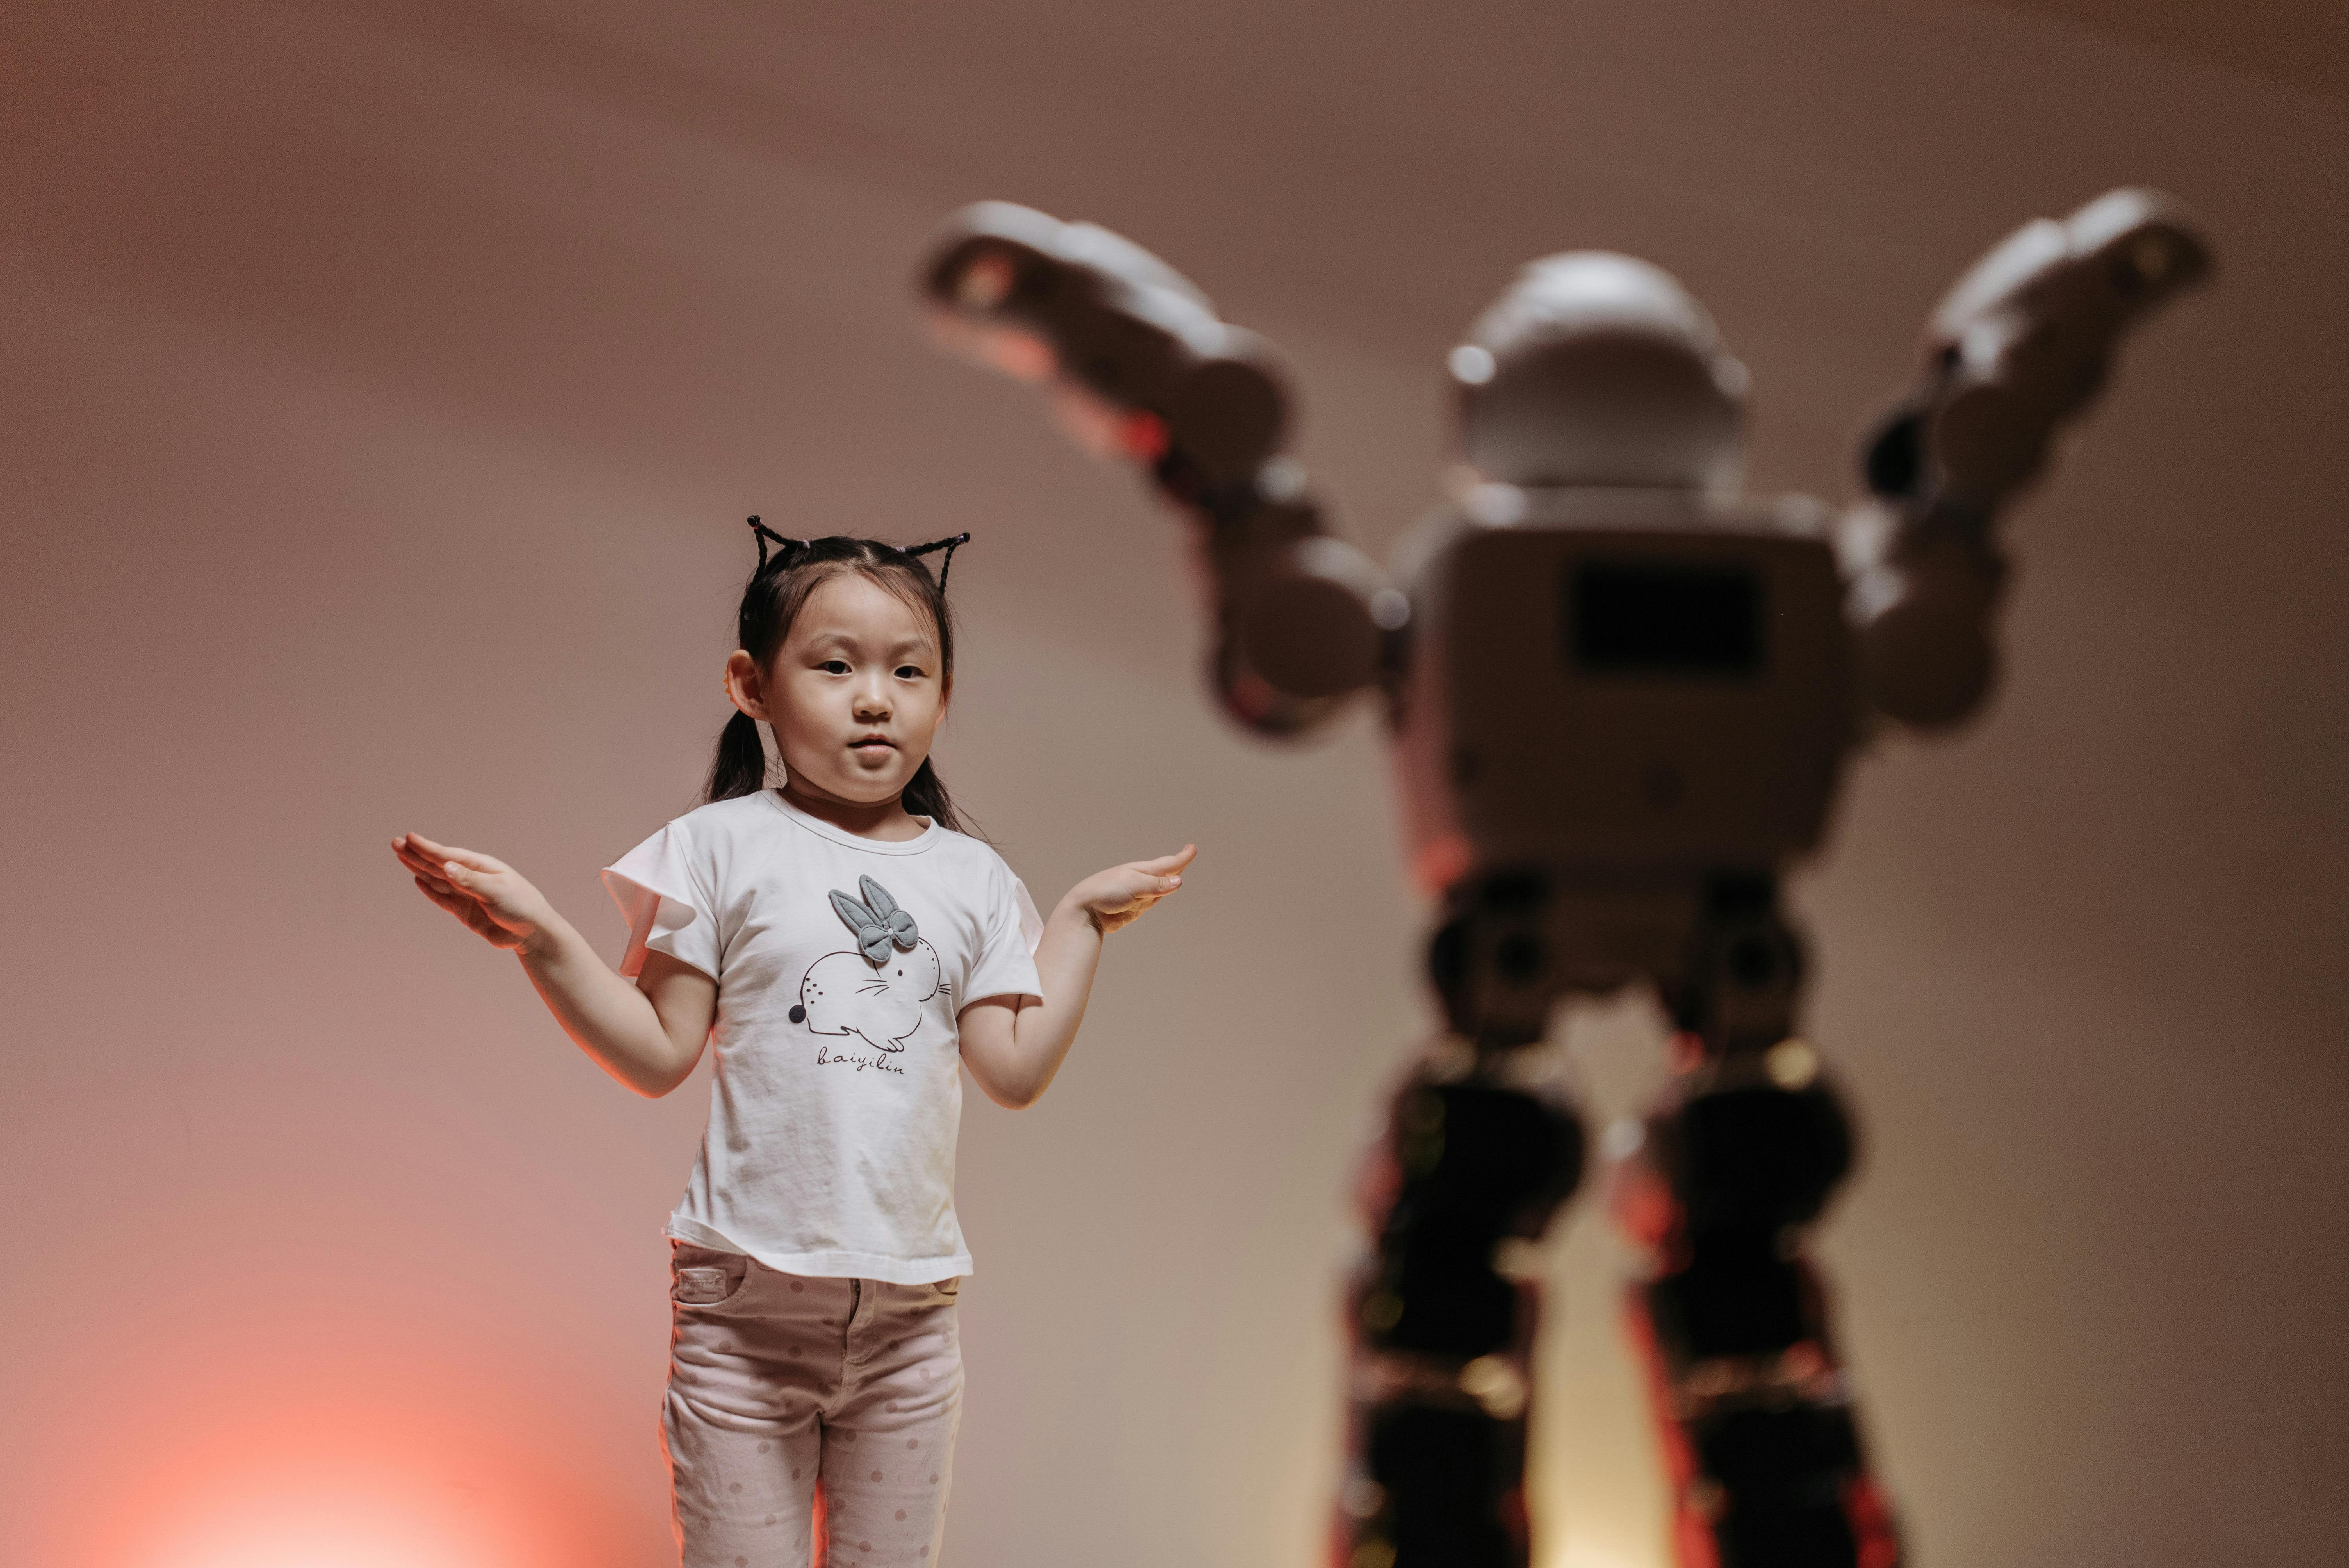
\includegraphics{./shared/robot-imitation-learning.jpg}

}

\caption{a robot imitating the pose of a young child (Photo by Pavel
Danilyuk:
https://www.pexels.com/photo/a-robot-imitating-a-girl-s-movement-8294811/)}

\end{figure}%

Now in machine learning, we are often trying to teach machines to
accomplish tasks that humans are already proficient at. In such cases,
the machine learning algorithm is the one learning the new skill, and
humans are the ``experts'' that can demonstrate how to perform the task.
\textbf{Imitation learning} is an approach to reinforcement learning
where we aim to learn a policy that performs at least as well as the
expert. It is often used as a first step for complex tasks where it is
impractical to learn from scratch.

We'll see that the most naive form of imitation learning, called
\textbf{behavioral cloning} (or ``behavior cloning''), is really an
application of supervised learning to interactive tasks. We'll then
explore \textbf{dataset aggregation} (DAgger) as a way to query an
expert and learn even more effectively.

\section{Behavioral cloning}\label{behavioral-cloning}

This notion of ``learning from human-provided data'' may remind you of
the basic premise of Chapter~\ref{sec-sl}. In supervised learning, there
is some mapping from \emph{inputs} to \emph{outputs}, such as the task
of assigning the correct label to an image, that humans can implicitly
compute. To teach a machine to calculate this mapping, we first collect
a large \emph{training dataset} by getting people to label a lot of
inputs, and then use some optimization algorithm to produce a predictor
that maps from the inputs to the outputs as closely as possible.

How does this relate to interactive tasks? Here, the input is the
observation seen by the agent and the output is the action it selects,
so the mapping is the agent's \emph{policy}. What's stopping us from
applying supervised learning techniques to mimic the expert's policy? In
principle, nothing! This is called \textbf{behavioral cloning}.

\begin{definition}[Behavioral
cloning]\protect\hypertarget{def-behavioral_cloning}{}\label{def-behavioral_cloning}

~

\begin{enumerate}
\def\labelenumi{\arabic{enumi}.}
\tightlist
\item
  Collect a training dataset of trajectories
  \(\mathcal{D} = (s^n, a^n)_{n=1}^{N}\) generated by an \textbf{expert
  policy} \(\pi_\text{expert}\). (For example, if the dataset contains
  \(M\) trajectories, each with a finite horizon \(H\), then
  \(N = M \times H\).)
\item
  Use a supervised learning algorithm
  \(\texttt{fit} : \mathcal{D} \mapsto \widetilde{\pi}\) to extract a
  policy \(\widetilde{\pi}\) that approximates the expert policy.
\end{enumerate}

\end{definition}

Typically, this second task can be framed as \textbf{empirical risk
minimization} (which we previously saw in
Definition~\ref{def-parameterized_empirical_risk_minimization}):

\[
\widetilde{\pi} = \arg\min_{\pi \in \Pi} \sum_{n=0}^{N-1} \text{loss}(\pi(s^n), a^n)
\]

where \(\Pi\) is some class of possible policies, \(\text{loss}\) is the
loss function to measure how different the policy's prediction is from
the true observed action, and the supervised learning algorithm itself,
also known as the \textbf{fitting method}, tells us how to compute this
\(\arg\min\).

How should we choose the loss function? In supervised learning, we saw
that the \textbf{mean squared error} is a good choice for continuous
outputs. However, how should we measure the difference between two
actions in a \emph{discrete} action space? In this setting, the policy
acts more like a \emph{classifier} that picks the best action in a given
state. Rather than considering a deterministic policy that just outputs
a single action, we'll consider a stochastic policy \(\pi\) that outputs
a \emph{distribution} over actions. This allows us to assign a
\emph{likelihood} to observing the entire dataset \(\mathcal{D}\) under
the policy \(\pi\), as if the state-action pairs are independent:

\[
\mathbb{P}_\pi(\mathcal{D}) = \prod_{n=1}^{N} \pi(a_n \mid s_n)
\]

Note that the states and actions are \emph{not}, however, actually
independent! A key property of interactive tasks is that the agent's
output -- the action that it takes -- may influence its next
observation. We want to find a policy under which the training dataset
\(\mathcal{D}\) is the most likely. This is called the \textbf{maximum
likelihood estimate} of the policy that generated the dataset:

\[
\widetilde{\pi} = \arg\max_{\pi \in \Pi} \mathbb{P}_{\pi}(\mathcal{D})
\]

This is also equivalent to doing empirical risk minimization with the
\textbf{negative log likelihood} as the loss function:

\[
\begin{aligned}
\widetilde{\pi} &= \arg\min_{\pi \in \Pi} - \log \mathbb{P}_\pi(\mathcal{D}) \\
&= \arg\min_{\pi \in \Pi} \sum_{n=1}^N - \log \pi(a_n \mid s_n)
\end{aligned}
\]

\subsection{Performance of behavioral
cloning}\label{performance-of-behavioral-cloning}

Can we quantify how well this algorithm works? For simplicity, let's
consider the case where the action space is \emph{finite} and both the
expert policy and learned policy are deterministic. Suppose the learned
policy obtains \(\varepsilon\) \emph{classification error}. That is, for
trajectories drawn from the expert policy, the learned policy chooses a
different action at most \(\varepsilon\) of the time:

\[
\mathbb{E}_{\tau \sim \rho_{\pi_{\text{expert}}}} \left[ \frac 1 H\sum_{h=0}^{H-1} \mathbf{1}\left\{ \widetilde{\pi}(s_h) \ne \pi_{\text{expert}} (s_h) \right\} \right] \le \varepsilon
\]

Then, their value functions differ by

\[
| V^{\pi_{\text{expert}}} - V^{\widetilde{\pi}} | \le H^2 \varepsilon
\]

where \(H\) is the horizon.

:::\{prf:theorem\} Performance of behavioral cloning

Recall the Performance Difference Lemma (Theorem~\ref{thm-pdl}) allows
us to express the difference between \(\pi_{\text{expert}}\) and
\(\widetilde{\pi}\) as

\begin{equation}\phantomsection\label{eq-pdl-rhs}{
V_0^{\pi_{\text{expert}}}(s) - V_0^{\widetilde{\pi}} (s) = \mathbb{E}_{\tau \sim \rho^{\pi_{\text{expert}}} \mid s_0 = s} \left[ \sum_{h=0}^{H-1} A_h^{\widetilde{\pi}} (s_h, a_h) \right].
}\end{equation}

Now since the expert policy is deterministic, we can substitute
\(a_h= \pi_{\text{expert}}(s_h)\). This allows us to make a further
simplification: since \(\pi_{\text{expert}}\) is deterministic, the
advantage of the chosen action is exactly zero:

\[
A^{\pi_{\text{expert}}}(s, \pi_{\text{expert}}(s)) = Q^{\pi_{\text{expert}}}(s, \pi_{\text{expert}}(s)) - V^{\pi_{\text{expert}}}(s) = 0.
\]

But the right-hand-side of Equation~\ref{eq-pdl-rhs} uses
\(A^{\widetilde{\pi}}\), not \(A^{\pi_{\text{expert}}}\). To bridge this
gap, we now use the assumption that \(\widetilde{\pi}\) obtains
\(\varepsilon\) classification error. Note that
\(A_h^{\widetilde{\pi}}(s_h, \pi_{\text{expert}}(s_h)) = 0\) when
\(\pi_{\text{expert}}(s_h) = \widetilde{\pi}(s_h)\). In the case where
the two policies differ on \(s_h\), which occurs with probability
\(\varepsilon\), the advantage is naively upper bounded by \(H\)
(assuming rewards are bounded between \(0\) and \(1\)). Taking the final
sum gives the desired bound. :::

\section{Distribution shift}\label{distribution-shift}

Let us return to the driving analogy. Suppose you have taken some
driving lessons and now feel comfortable in your neighbourhood. But
today you have to travel to an area you haven't visited before, such as
a highway, where it would be dangerous to try and apply the techniques
you've already learned. This is the issue of \emph{distribution shift}:
a policy learned under a certain distribution of states may not perform
well if this distribution changes.

This is already a common issue in supervised learning, where the
training dataset for a model might not resemble the environment where it
gets deployed. In interactive environments, this issue is further
exacerbated by the dependency between the observations and the agent's
behavior; if you take a wrong turn early on, it may be difficult or
impossible to recover in that trajectory.

How could you learn a strategy for these new settings? In the driving
example, you might decide to install a dashcam to record the car's
surroundings. That way, once you make it back to safety, you can show
the recording to an expert, who can provide feedback at each step of the
way. Then the next time you go for a drive, you can remember the
expert's advice, and take a safer route. You could then repeat this
training as many times as desired, thereby collecting the expert's
feedback over a diverse range of locations. This is the key idea behind
\emph{dataset aggregation}.

\section{Dataset aggregation (DAgger)}\label{dataset-aggregation-dagger}

The DAgger algorithm (Ross, Gordon, and Bagnell (2010)) assumes that we
have \emph{query access} to the expert policy. That is, for a given
state \(s\), we can ask for the expert's action
\(\pi_{\text{expert}}(s)\) in that state. We also need access to the
environment for rolling out policies. This makes DAgger an
\textbf{online} algorithm, as opposed to pure behavioral cloning, which
is \textbf{offline} since we don't need to act in the environment at
all.

You can think of DAgger as a specific way of collecting the dataset
\(\mathcal{D}\).

:::\{prf:algorithm\} DAgger

Inputs: \(\pi_{\text{expert}}\), an initial policy
\(\pi_{\text{init}}\), the number of iterations \(T\), and the number of
trajectories \(N\) to collect per iteration.

\begin{enumerate}
\def\labelenumi{\arabic{enumi}.}
\tightlist
\item
  Initialize \(\mathcal{D} = \{\}\) (the empty set) and
  \(\pi = \pi_{\text{init}}\).
\item
  For \(t = 1, \dots, T\):

  \begin{itemize}
  \tightlist
  \item
    Collect \(N\) trajectories \(\tau_1, \dots, \tau_N\) using the
    current policy \(\pi\).
  \item
    For each trajectory \(\tau_n\):

    \begin{itemize}
    \tightlist
    \item
      Replace each action \(a_h\) in \(\tau_n\) with the \textbf{expert
      action} \(\pi_{\text{expert}}(s_h)\).
    \item
      Call the resulting trajectory \(\tau^{\text{expert}}_n\).
    \end{itemize}
  \item
    \(\mathcal{D} \gets \mathcal{D} \cup \{ \tau^{\text{expert}}_1, \dots, \tau^{\text{expert}}_n \}\).
  \item
    Let \(\pi \gets \texttt{fit}(\mathcal{D})\), where \(\texttt{fit}\)
    is a behavioral cloning algorithm.
  \end{itemize}
\item
  Return \(\pi\). :::
\end{enumerate}

We leave the implementation as an exercise. How well does DAgger
perform? A full proof can be found in Ross, Gordon, and Bagnell (2010)
that under certain assumptions, the DAgger algorithm can better
approximate the expert policy:

\[
|V^{\pi_{\text{expert}}} - V^{\pi_{\text{DAgger}}}| \le H \varepsilon
\]

where \(\varepsilon\) is the ``classification error'' guaranteed by the
supervised learning algorithm.

\section{Summary}\label{summary-5}

For tasks where it is too difficult or expensive to learn from scratch,
we can instead start off with a collection of \textbf{expert
demonstrations}. Then we can use supervised learning techniques to find
a policy that imitates the expert demonstrations.

The simplest way to do this is to apply a supervised learning algorithm
to an already-collected dataset of expert state-action pairs. This is
called \textbf{behavioral cloning}. However, given query access to the
expert policy, we can do better by integrating its feedback in an online
loop. The \textbf{DAgger} algorithm is one way of doing this, where we
use the expert policy to augment trajectories and then learn from this
augmented dataset using behavioral cloning.

\bookmarksetup{startatroot}

\chapter{Tree Search Methods}\label{sec-planning}

\begin{center}\rule{0.5\linewidth}{0.5pt}\end{center}

\begin{center}\rule{0.5\linewidth}{0.5pt}\end{center}

\section{Introduction}\label{introduction-8}

Have you ever lost a strategy game against a skilled opponent? It
probably seemed like they were \emph{ahead of you at every turn}. They
might have been \emph{planning ahead} and anticipating your actions,
then formulating their strategy to counter yours. If this opponent was a
computer, they might have been using one of the strategies that we are
about to explore.

\begin{Shaded}
\begin{Highlighting}[]
\OperatorTok{\%}\NormalTok{load\_ext autoreload}
\OperatorTok{\%}\NormalTok{autoreload }\DecValTok{2}
\end{Highlighting}
\end{Shaded}

\begin{Shaded}
\begin{Highlighting}[]
\ImportTok{from}\NormalTok{ utils }\ImportTok{import}\NormalTok{ Int, Array, latex, jnp, NamedTuple}
\ImportTok{from}\NormalTok{ enum }\ImportTok{import}\NormalTok{ IntEnum}
\end{Highlighting}
\end{Shaded}

\section{Deterministic, zero sum, fully observable two-player
games}\label{deterministic-zero-sum-fully-observable-two-player-games}

In this chapter, we will focus on games that are:

\begin{itemize}
\tightlist
\item
  \emph{deterministic,}
\item
  \emph{zero sum} (one player wins and the other loses),
\item
  \emph{fully observable,} that is, the state of the game is perfectly
  known by both players,
\item
  for \emph{two players} that alternate turns,
\end{itemize}

We can represent such a game as a \emph{complete game tree.} Each
possible state is a node in the tree, and since we only consider
deterministic games, we can represent actions as edges leading from the
current state to the next. Each path through the tree, from root to
leaf, represents a single game.

:::\{figure\} shared/tic\_tac\_toe.png :align: center

The first two layers of the complete game tree of tic-tac-toe. From
Wikimedia. :::

If you could store the complete game tree on a computer, you would be
able to win every potentially winnable game by searching all paths from
your current state and taking a winning move. We will see an explicit
algorithm for this in Section~\ref{sec-min-max-search}. However, as
games become more complex, it becomes computationally impossible to
search every possible path.

For instance, a chess player has roughly 30 actions to choose from at
each turn, and each game takes roughly 40 moves per player, so trying to
solve chess exactly using minimax would take somewhere on the order of
\(30^{80} \approx 10^{118}\) operations. That's 10 billion billion
billion billion billion billion billion billion billion billion billion
billion billion operations. As of the time of writing, the fastest
processor can achieve almost 10 GHz (10 billion operations per second),
so to fully solve chess using minimax is many, many orders of magnitude
out of reach.

It is thus intractable, in any realistic setting, to solve the complete
game tree exactly. Luckily, only a small fraction of those games ever
occur in reality; Later in this chapter, we will explore ways to
\emph{prune away} parts of the tree that we know we can safely ignore.
We can also \emph{approximate} the value of a state without fully
evaluating it. Using these approximations, we can no longer
\emph{guarantee} winning the game, but we can come up with strategies
that will do well against most opponents.

\subsection{Notation}\label{notation-1}

Let us now describe these games formally. We'll call the first player
Max and the second player Min. Max seeks to maximize the final game
score, while Min seeks to minimize the final game score.

\begin{itemize}
\tightlist
\item
  We'll use \(\mathcal{S}\) to denote the set of all possible game
  states.
\item
  The game begins in some \textbf{initial state}
  \(s_0 \in \mathcal{S}\).
\item
  Max moves on even turn numbers \(h = 2n\), and Min moves on odd turn
  numbers \(h = 2n+1\), where \(n\) is a natural number.
\item
  The space of possible actions, \(\mathcal{A}_h(s)\), depends on the
  state itself, as well as whose turn it is. (For example, in
  tic-tac-toe, Max can only play \texttt{X}s while Min can only play
  \texttt{O}s.)
\item
  The game ends after \(H\) total moves (which might be even or odd). We
  call the final state a \textbf{terminal state}.
\item
  \(P\) denotes the \textbf{state transitions}, that is, \(P(s, a)\)
  denotes the resulting state when taking action
  \(a \in \mathcal{A}(s)\) in state \(s\). We'll assume that this
  function is time-homogeneous (a.k.a. stationary) and doesn't change
  across timesteps.
\item
  \(r(s)\) denotes the \textbf{game score} of the terminal state \(s\).
  Note that this is some positive or negative value seen by both
  players: A positive value indicates Max winning, a negative value
  indicates Min winning, and a value of \(0\) indicates a tie.
\end{itemize}

We also call the sequence of states and actions a \textbf{trajectory}.

Above, we suppose that the game ends after \(H\) total moves. But most
real games have a \emph{variable} length. How would you describe this?

\begin{example}[Tic-tac-toe]\protect\hypertarget{exm-tic-tac-toe}{}\label{exm-tic-tac-toe}

Let us frame tic-tac-toe in this setting.

\begin{itemize}
\tightlist
\item
  Each of the \(9\) squares is either empty, marked X, or marked O. So
  there are \(|\mathcal{S}| = 3^9\) potential states. Not all of these
  may be reachable!
\item
  The initial state \(s_0\) is the empty board.
\item
  The set of possible actions for Max in state \(s\),
  \(\mathcal{A}_{2n}(s)\), is the set of tuples \((\text{``X''}, i)\)
  where \(i\) refers to an empty square in \(s\). Similarly,
  \(\mathcal{A}_{2n+1}(s)\) is the set of tuples \((\text{``O''}, i)\)
  where \(i\) refers to an empty square in \(s\).
\item
  We can take \(H = 9\) as the longest possible game length.
\item
  \(P(s, a)\) for a \emph{nonterminal} state \(s\) is simply the board
  with the symbol and square specified by \(a\) marked into \(s\).
  Otherwise, if \(s\) is a \emph{terminal} state, i.e.~it already has
  three symbols in a row, the state no longer changes.
\item
  \(r(s)\) at a \emph{terminal} state is \(+1\) if there are three Xs in
  a row, \(-1\) if there are three Os in a row, and \(0\) otherwise.
\end{itemize}

\end{example}

Our notation may remind you of Chapter~\ref{sec-mdps}. Given that these
games also involve a sequence of states and actions, can we formulate
them as finite-horizon MDPs? The two settings are not exactly analogous,
since in MDPs we only consider a \emph{single} policy, while these games
involve two distinct players with opposite objectives. Since we want to
analyze the behavior of \emph{both} players at the same time, describing
such a game as an MDP is more trouble than it's worth.

\begin{Shaded}
\begin{Highlighting}[]
\KeywordTok{class}\NormalTok{ Player(IntEnum):}
\NormalTok{    EMPTY }\OperatorTok{=} \DecValTok{0}
\NormalTok{    X }\OperatorTok{=} \DecValTok{1}
\NormalTok{    O }\OperatorTok{=} \DecValTok{2}


\ControlFlowTok{if} \VariableTok{False}\NormalTok{:}
    \KeywordTok{class}\NormalTok{ TicTacToeEnv(gym.Env):}
\NormalTok{        metadata }\OperatorTok{=}\NormalTok{ \{}\StringTok{"render.modes"}\NormalTok{: [}\StringTok{"human"}\NormalTok{]\}}

        \KeywordTok{def} \FunctionTok{\_\_init\_\_}\NormalTok{(}\VariableTok{self}\NormalTok{):}
            \BuiltInTok{super}\NormalTok{().}\FunctionTok{\_\_init\_\_}\NormalTok{()}
            \VariableTok{self}\NormalTok{.action\_space }\OperatorTok{=}\NormalTok{ spaces.Discrete(}\DecValTok{9}\NormalTok{)}
            \VariableTok{self}\NormalTok{.observation\_space }\OperatorTok{=}\NormalTok{ spaces.Box(}
\NormalTok{                low}\OperatorTok{=}\DecValTok{0}\NormalTok{, high}\OperatorTok{=}\DecValTok{2}\NormalTok{, shape}\OperatorTok{=}\NormalTok{(}\DecValTok{3}\NormalTok{, }\DecValTok{3}\NormalTok{), dtype}\OperatorTok{=}\NormalTok{jnp.int32}
\NormalTok{            )}
            \VariableTok{self}\NormalTok{.board }\OperatorTok{=} \VariableTok{None}
            \VariableTok{self}\NormalTok{.current\_player }\OperatorTok{=} \VariableTok{None}
            \VariableTok{self}\NormalTok{.done }\OperatorTok{=} \VariableTok{None}

        \KeywordTok{def}\NormalTok{ reset(}\VariableTok{self}\NormalTok{, seed}\OperatorTok{=}\VariableTok{None}\NormalTok{, options}\OperatorTok{=}\VariableTok{None}\NormalTok{):}
            \BuiltInTok{super}\NormalTok{().reset(seed}\OperatorTok{=}\NormalTok{seed)}
            \VariableTok{self}\NormalTok{.board }\OperatorTok{=}\NormalTok{ jnp.zeros((}\DecValTok{3}\NormalTok{, }\DecValTok{3}\NormalTok{), dtype}\OperatorTok{=}\NormalTok{jnp.int32)}
            \VariableTok{self}\NormalTok{.current\_player }\OperatorTok{=}\NormalTok{ Player.X}
            \VariableTok{self}\NormalTok{.done }\OperatorTok{=} \VariableTok{False}
            \ControlFlowTok{return} \VariableTok{self}\NormalTok{.board, \{\}}

        \KeywordTok{def}\NormalTok{ step(}\VariableTok{self}\NormalTok{, action: jnp.int32) }\OperatorTok{{-}\textgreater{}}\NormalTok{ Int[Array, }\StringTok{"3 3"}\NormalTok{]:}
            \CommentTok{"""Take the action a in state s."""}
            \ControlFlowTok{if} \VariableTok{self}\NormalTok{.done:}
                \ControlFlowTok{raise} \PreprocessorTok{ValueError}\NormalTok{(}\StringTok{"The game is already over. Call \textasciigrave{}env.reset()\textasciigrave{} to reset the environment."}\NormalTok{)}
            
\NormalTok{            row, col }\OperatorTok{=} \BuiltInTok{divmod}\NormalTok{(action, }\DecValTok{3}\NormalTok{)}
            \ControlFlowTok{if} \VariableTok{self}\NormalTok{.board[row, col] }\OperatorTok{!=}\NormalTok{ Player.EMPTY:}
                \ControlFlowTok{return} \VariableTok{self}\NormalTok{.board, }\OperatorTok{{-}}\DecValTok{10}
            \ControlFlowTok{return}\NormalTok{ s.at[row, col].}\BuiltInTok{set}\NormalTok{(player)}

        \AttributeTok{@staticmethod}
        \KeywordTok{def}\NormalTok{ is\_terminal(s: Int[Array, }\StringTok{"3 3"}\NormalTok{]):}
            \CommentTok{"""Check if the game is over."""}
            \ControlFlowTok{return}\NormalTok{ is\_winner(s, Player.X) }\KeywordTok{or}\NormalTok{ is\_winner(s, Player.O) }\KeywordTok{or}\NormalTok{ jnp.}\BuiltInTok{all}\NormalTok{(s }\OperatorTok{==}\NormalTok{ Player.EMPTY)}

        \AttributeTok{@staticmethod}
        \KeywordTok{def}\NormalTok{ is\_winner(board: Int[Array, }\StringTok{"3 3"}\NormalTok{], player: Player):}
            \CommentTok{"""Check if the given player has won."""}
            \ControlFlowTok{return} \BuiltInTok{any}\NormalTok{(}
\NormalTok{                jnp.}\BuiltInTok{all}\NormalTok{(board[i, :] }\OperatorTok{==}\NormalTok{ player) }\KeywordTok{or}
\NormalTok{                jnp.}\BuiltInTok{all}\NormalTok{(board[:, i] }\OperatorTok{==}\NormalTok{ player)}
                \ControlFlowTok{for}\NormalTok{ i }\KeywordTok{in} \BuiltInTok{range}\NormalTok{(}\DecValTok{3}\NormalTok{)}
\NormalTok{            ) }\KeywordTok{or}\NormalTok{ jnp.}\BuiltInTok{all}\NormalTok{(jnp.diag(board) }\OperatorTok{==}\NormalTok{ player) }\KeywordTok{or}\NormalTok{ jnp.}\BuiltInTok{all}\NormalTok{(jnp.diag(jnp.fliplr(board)) }\OperatorTok{==}\NormalTok{ player)}

        \AttributeTok{@staticmethod}
        \KeywordTok{def}\NormalTok{ show(s: Int[Array, }\StringTok{"3 3"}\NormalTok{]):}
            \CommentTok{"""Print the board."""}
            \ControlFlowTok{for}\NormalTok{ row }\KeywordTok{in} \BuiltInTok{range}\NormalTok{(}\DecValTok{3}\NormalTok{):}
                \BuiltInTok{print}\NormalTok{(}\StringTok{" | "}\NormalTok{.join(}\StringTok{" XO"}\NormalTok{[s[row, col]] }\ControlFlowTok{for}\NormalTok{ col }\KeywordTok{in} \BuiltInTok{range}\NormalTok{(}\DecValTok{3}\NormalTok{)))}
                \ControlFlowTok{if}\NormalTok{ row }\OperatorTok{\textless{}} \DecValTok{2}\NormalTok{:}
                    \BuiltInTok{print}\NormalTok{(}\StringTok{"{-}"} \OperatorTok{*} \DecValTok{5}\NormalTok{)}
\end{Highlighting}
\end{Shaded}

\section{Min-max search}\label{sec-min-max-search}

In the introduction, we claimed that we could win any potentially
winnable game by looking ahead and predicting the opponent's actions.
This would mean that each \emph{nonterminal} state already has some
predetermined game score, that is, in each state, it is already
``obvious'' which player is going to win.

Let \(V_h^\star(s)\) denote the game score under optimal play from both
players starting in state \(s\) at time \(h\).

\begin{definition}[Min-max search
algorithm]\protect\hypertarget{def-min-max-value}{}\label{def-min-max-value}

\[
V_h^{\star}(s) = \begin{cases}
r(s) & h= H\\
\max_{a \in \mathcal{A}_h(s)} V_{h+1}^{\star}(P(s, a)) & h\text{ is even and } h< H \\
\min_{a \in \mathcal{A}_h(s)} V_{h+1}^{\star}(P(s, a)) & h\text{ is odd and } h< H \\
\end{cases}
\]

\end{definition}

We can compute this by starting at the terminal states, when the game's
outcome is known, and working backwards, assuming that Max chooses the
action that leads to the highest score and Min chooses the action that
leads to the lowest score.

This translates directly into a recursive depth-first search algorithm
for searching the complete game tree.

\begin{Shaded}
\begin{Highlighting}[]
\KeywordTok{def}\NormalTok{ minimax\_search(s, player) }\OperatorTok{{-}\textgreater{}} \BuiltInTok{tuple}\NormalTok{[}\StringTok{"Action"}\NormalTok{, }\StringTok{"Value"}\NormalTok{]:}
    \CommentTok{\# Return the value of the state (for Max) and the best action for Max to take.}
    \ControlFlowTok{if}\NormalTok{ env.is\_terminal(s):}
        \ControlFlowTok{return} \VariableTok{None}\NormalTok{, env.winner(s)}

    \ControlFlowTok{if}\NormalTok{ player }\KeywordTok{is} \BuiltInTok{max}\NormalTok{:}
\NormalTok{        a\_max, v\_max }\OperatorTok{=} \VariableTok{None}\NormalTok{, }\VariableTok{None}
        \ControlFlowTok{for}\NormalTok{ a }\KeywordTok{in}\NormalTok{ env.action\_space(s):}
\NormalTok{            \_, v }\OperatorTok{=}\NormalTok{ minimax\_search(env.step(s, a), }\BuiltInTok{min}\NormalTok{)}
            \ControlFlowTok{if}\NormalTok{ v }\OperatorTok{\textgreater{}}\NormalTok{ v\_max:}
\NormalTok{                a\_max, v\_max }\OperatorTok{=}\NormalTok{ a, v}
        \ControlFlowTok{return}\NormalTok{ a\_max, v\_max}
    \ControlFlowTok{else}\NormalTok{:}
\NormalTok{        a\_min, v\_min }\OperatorTok{=} \VariableTok{None}\NormalTok{, }\VariableTok{None}
        \ControlFlowTok{for}\NormalTok{ a }\KeywordTok{in}\NormalTok{ env.action\_space(s):}
\NormalTok{            \_, v }\OperatorTok{=}\NormalTok{ minimax\_search(env.step(s, a), }\BuiltInTok{max}\NormalTok{)}
            \ControlFlowTok{if}\NormalTok{ v }\OperatorTok{\textless{}}\NormalTok{ v\_min:}
\NormalTok{                a\_min, v\_min }\OperatorTok{=}\NormalTok{ a, v}
        \ControlFlowTok{return}\NormalTok{ a\_min, v\_min}

\NormalTok{latex(minimax\_search, custom\_identifiers}\OperatorTok{=}\NormalTok{\{}\StringTok{"env.step"}\NormalTok{: }\StringTok{"P"}\NormalTok{, }\StringTok{"env.action\_space"}\NormalTok{: }\VerbatimStringTok{r"\textbackslash{}mathcal}\SpecialCharTok{\{A\}}\VerbatimStringTok{"}\NormalTok{\})}
\end{Highlighting}
\end{Shaded}

$ \begin{array}{l} \mathbf{function} \ \mathrm{minimax\_search}(s, \mathrm{player}) \\ \hspace{1em} \mathbf{if} \ \mathrm{env}.\mathrm{is\_terminal} \mathopen{}\left( s \mathclose{}\right) \\ \hspace{2em} \mathbf{return} \ \mathopen{}\left( \mathrm{None}, \mathrm{env}.\mathrm{winner} \mathopen{}\left( s \mathclose{}\right) \mathclose{}\right) \\ \hspace{1em} \mathbf{end \ if} \\ \hspace{1em} \mathbf{if} \ \mathrm{player} \equiv \mathrm{max} \\ \hspace{2em} \mathopen{}\left( \mathrm{a\_max}, \mathrm{v\_max} \mathclose{}\right) \gets \mathopen{}\left( \mathrm{None}, \mathrm{None} \mathclose{}\right) \\ \hspace{2em} \mathbf{for} \ a \in \mathrm{env}.\mathrm{action\_space} \mathopen{}\left( s \mathclose{}\right) \ \mathbf{do} \\ \hspace{3em} \mathopen{}\left( \mathrm{\_}, v \mathclose{}\right) \gets \mathrm{minimax\_search} \mathopen{}\left( \mathrm{env}.\mathrm{step} \mathopen{}\left( s, a \mathclose{}\right), \mathrm{min} \mathclose{}\right) \\ \hspace{3em} \mathbf{if} \ v > \mathrm{v\_max} \\ \hspace{4em} \mathopen{}\left( \mathrm{a\_max}, \mathrm{v\_max} \mathclose{}\right) \gets \mathopen{}\left( a, v \mathclose{}\right) \\ \hspace{3em} \mathbf{end \ if} \\ \hspace{2em} \mathbf{end \ for} \\ \hspace{2em} \mathbf{return} \ \mathopen{}\left( \mathrm{a\_max}, \mathrm{v\_max} \mathclose{}\right) \\ \hspace{1em} \mathbf{else} \\ \hspace{2em} \mathopen{}\left( \mathrm{a\_min}, \mathrm{v\_min} \mathclose{}\right) \gets \mathopen{}\left( \mathrm{None}, \mathrm{None} \mathclose{}\right) \\ \hspace{2em} \mathbf{for} \ a \in \mathrm{env}.\mathrm{action\_space} \mathopen{}\left( s \mathclose{}\right) \ \mathbf{do} \\ \hspace{3em} \mathopen{}\left( \mathrm{\_}, v \mathclose{}\right) \gets \mathrm{minimax\_search} \mathopen{}\left( \mathrm{env}.\mathrm{step} \mathopen{}\left( s, a \mathclose{}\right), \mathrm{max} \mathclose{}\right) \\ \hspace{3em} \mathbf{if} \ v < \mathrm{v\_min} \\ \hspace{4em} \mathopen{}\left( \mathrm{a\_min}, \mathrm{v\_min} \mathclose{}\right) \gets \mathopen{}\left( a, v \mathclose{}\right) \\ \hspace{3em} \mathbf{end \ if} \\ \hspace{2em} \mathbf{end \ for} \\ \hspace{2em} \mathbf{return} \ \mathopen{}\left( \mathrm{a\_min}, \mathrm{v\_min} \mathclose{}\right) \\ \hspace{1em} \mathbf{end \ if} \\ \mathbf{end \ function} \end{array} $

\begin{example}[Min-max search for a simple
game]\protect\hypertarget{exm-min-max-example}{}\label{exm-min-max-example}

Consider a simple game with just two steps: Max chooses one of three
possible actions (A, B, C), and then Min chooses one of three possible
actions (D, E, F). The combination leads to a certain integer outcome,
shown in the table below:

\begin{longtable}[]{@{}llll@{}}
\toprule\noalign{}
& D & E & F \\
\midrule\noalign{}
\endhead
\bottomrule\noalign{}
\endlastfoot
A & 4 & -2 & 5 \\
B & -3 & 3 & 1 \\
C & 0 & 3 & -1 \\
\end{longtable}

We can visualize this as the following complete game tree, where each
box contains the value \(V_h^\star(s)\) of that node. The min-max values
of the terminal states are already known:

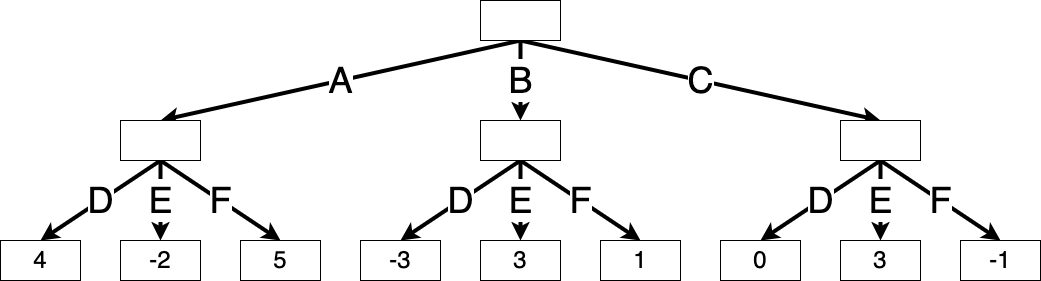
\includegraphics{./shared/minmax.png}

We begin min-max search at the root, exploring each of Max's actions.
Suppose Max chooses action A. Then Min will choose action E to minimize
the game score, making the value of this game node
\(\min(4, -2, 5) = -2\).

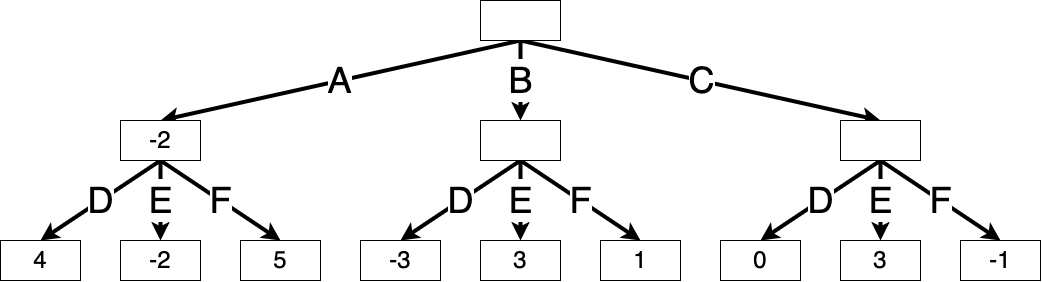
\includegraphics{./shared/minmax-2.png}

Similarly, if Max chooses action B, then Min will choose action D, and
if Max chooses action C, then Min will choose action F. We can fill in
the values of these nodes accordingly:

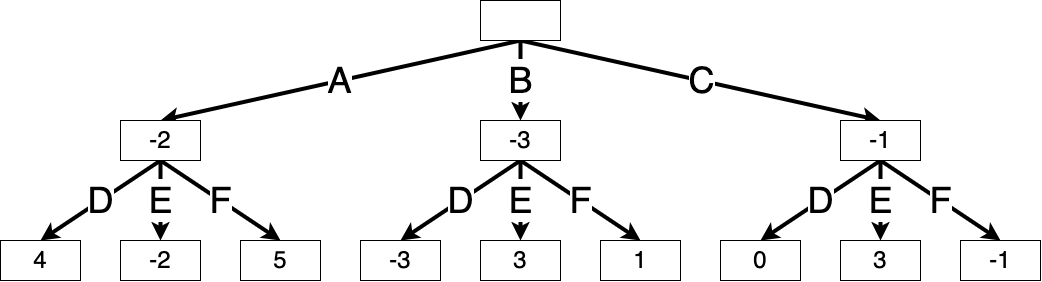
\includegraphics{./shared/minmax-3.png}

Thus, Max's best move is to take action C, resulting in a game score of
\(\max(-2, -3, -1) = -1\).

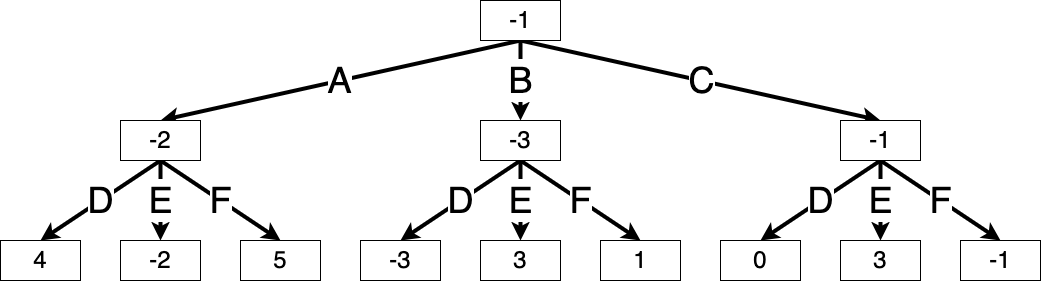
\includegraphics{./shared/minmax-4.png}

\end{example}

\subsection{Complexity of min-max
search}\label{complexity-of-min-max-search}

At each of the \(H\) timesteps, this algorithm iterates through the
entire action space at that state, and therefore has a time complexity
of \(H^{n_A}\) (where \(n_A\) is the largest number of actions possibly
available at once). This makes the min-max algorithm impractical for
even moderately sized games.

But do we need to compute the exact value of \emph{every} possible
state? Instead, is there some way we could ``ignore'' certain actions
and their subtrees if we already know of better options? The
\textbf{alpha-beta search} makes use of this intuition.

\section{Alpha-beta search}\label{sec-alpha-beta-search}

The intuition behind alpha-beta search is as follows: Suppose Max is in
state \(s\), and considering whether to take action \(a\) or \(a'\). If
at any point they find out that action \(a'\) is definitely worse than
(or equal to) action \(a\), they don't need to evaluate action \(a'\)
any further.

Concretely, we run min-max search as above, except now we keep track of
two additional parameters \(\alpha(s)\) and \(\beta(s)\) while
evaluating each state:

\begin{itemize}
\tightlist
\item
  Starting in state \(s\), Max can achieve a game score of \emph{at
  least} \(\alpha(s)\) assuming Min plays optimally. That is,
  \(V^\star_h(s) \ge \alpha(s)\) at all points.
\item
  Analogously, starting in state \(s\), Min can ensure a game score of
  \emph{at most} \(\beta(s)\) assuming Max plays optimally. That is,
  \(V^\star_h(s) \le \beta(s)\) at all points.
\end{itemize}

Suppose we are evaluating \(V^\star_h(s)\), where it is Max's turn
(\(h\) is even). We update \(\alpha(s)\) to be the \emph{highest}
minimax value achievable from \(s\) so far. That is, the value of \(s\)
is \emph{at least} \(\alpha(s)\). Suppose Max chooses action \(a\),
which leads to state \(s'\), in which it is Min's turn. If any of Min's
actions in \(s'\) achieve a value \(V^\star_{h+1}(s') \le \alpha(s)\),
we know that Max would not choose action \(a\), since they know that it
is \emph{worse} than whichever action gave the value \(\alpha(s)\).
Similarly, to evaluate a state on Min's turn, we update \(\beta(s)\) to
be the \emph{lowest} value achievable from \(s\) so far. That is, the
value of \(s\) is \emph{at most} \(\beta(s)\). Suppose Min chooses
action \(a\), which leads to state \(s'\) for Max. If Max has any
actions that do \emph{better} than \(\beta(s)\), they would take it,
making action \(a\) a suboptimal choice for Min.

\begin{example}[Alpha-beta search for a simple
game]\protect\hypertarget{exm-alpha-beta-example}{}\label{exm-alpha-beta-example}

Let us use the same simple game from Example~\ref{exm-min-max-example}.
We list the values of \(\alpha(s), \beta(s)\) in each node throughout
the algorithm. These values are initialized to \(-\infty, +\infty\)
respectively. We shade any squares that have not been visited by the
algorithm, and we assume that actions are evaluated from left to right.

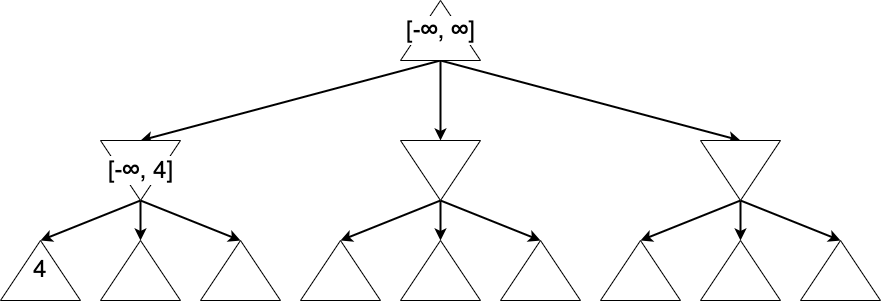
\includegraphics{./shared/alpha-beta-0.png}

Suppose Max takes action A. Let \(s'\) be the resulting game state. The
values of \(\alpha(s')\) and \(\beta(s')\) are initialized at the same
values as the root state, since we want to prune a subtree if there
exists a better action at any step higher in the tree.

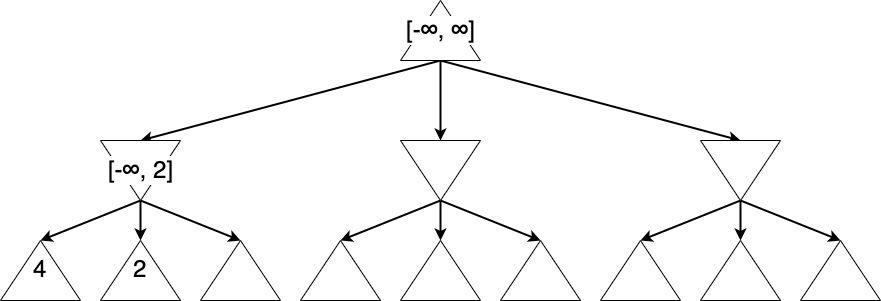
\includegraphics{./shared/alpha-beta-1.png}

Then we iterate through Min's possible actions, updating the value of
\(\beta(s')\) as we go.

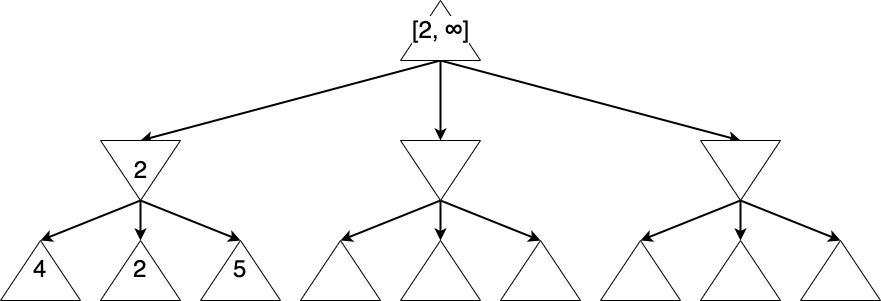
\includegraphics{./shared/alpha-beta-2.png}
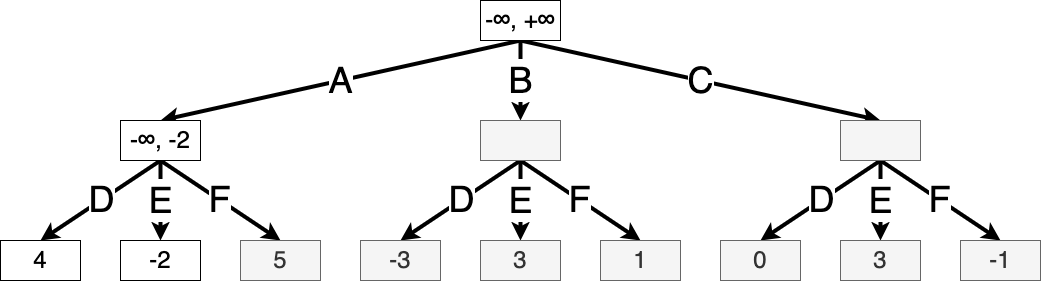
\includegraphics{./shared/alpha-beta-3.png}

Once the value of state \(s'\) is fully evaluated, we know that Max can
achieve a value of \emph{at least} \(-2\) starting from the root, and so
we update \(\alpha(s)\), where \(s\) is the root state:

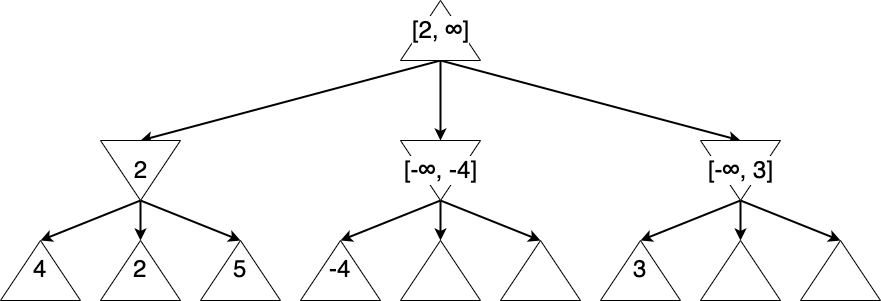
\includegraphics{./shared/alpha-beta-4.png}

Then Max imagines taking action B. Again, let \(s'\) denote the
resulting game state. We initialize \(\alpha(s')\) and \(\beta(s')\)
from the root:

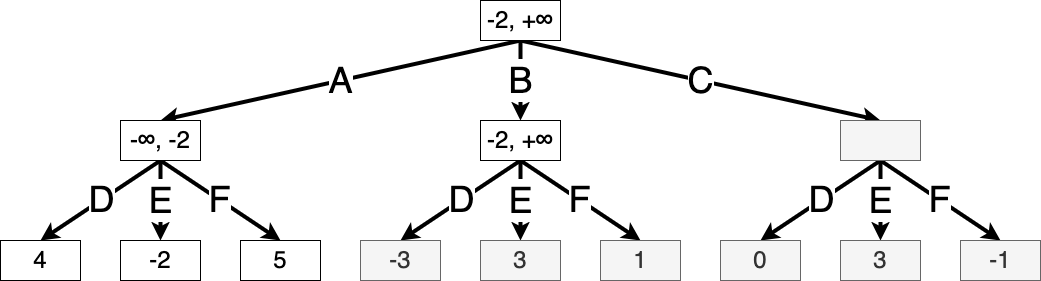
\includegraphics{./shared/alpha-beta-5.png}

Now suppose Min takes action D, resulting in a value of \(-3\). We see
that \(V^\star_h(s') = \min(-3, x, y)\), where \(x\) and \(y\) are the
values of the remaining two actions. But since
\(\min(-3, x, y) \le -3\), we know that the value of \(s'\) is at most
\(-3\). But Max can achieve a better value of \(\alpha(s') = -2\) by
taking action A, and so Max will never take action B, and we can prune
the search here. We will use dotted lines to indicate states that have
been ruled out from the search:

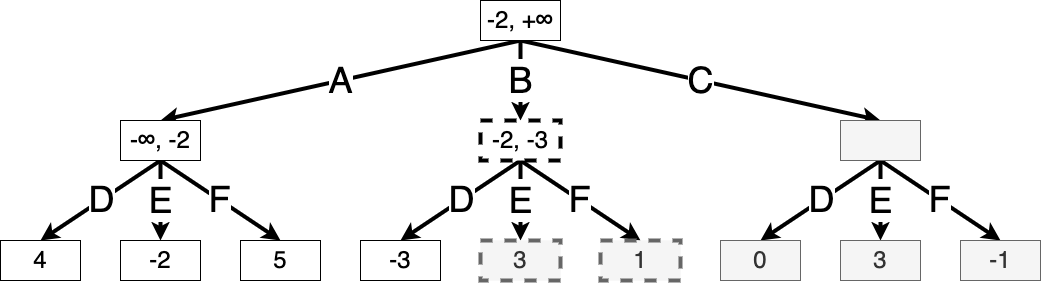
\includegraphics{./shared/alpha-beta-6.png}

Finally, suppose Max takes action C. For Min's actions D and E, there is
still a chance that action C might outperform action A, so we continue
expanding:

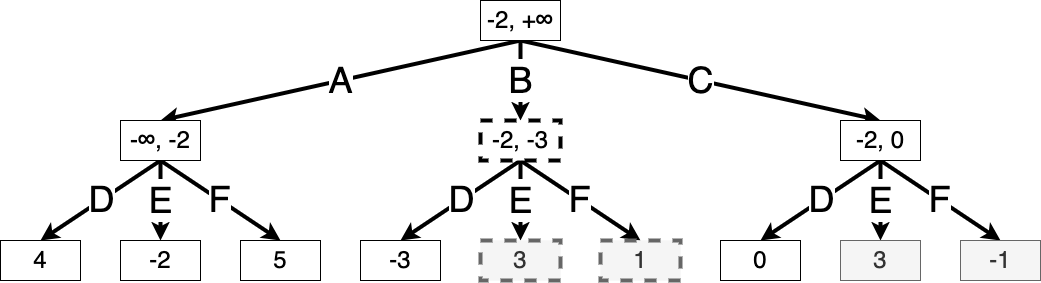
\includegraphics{./shared/alpha-beta-7.png}
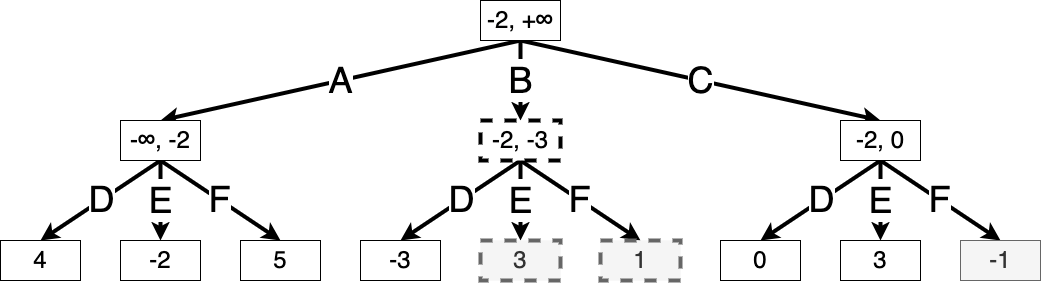
\includegraphics{./shared/alpha-beta-8.png}

Finally, we see that Min taking action F achieves the minimum value at
this state. This shows that optimal play is for Max to take action C,
and Min to take action F.

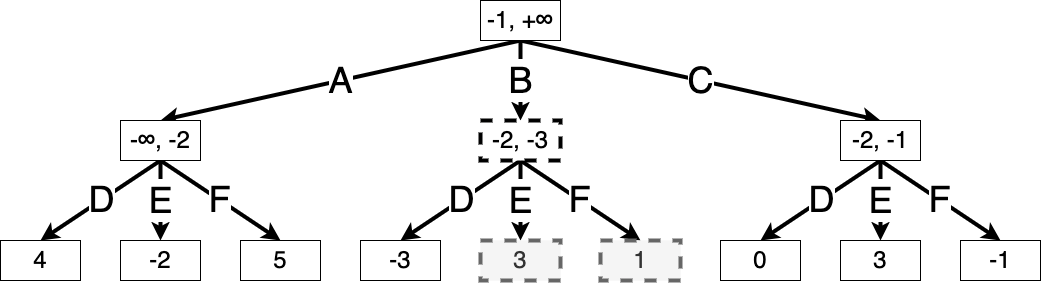
\includegraphics{./shared/alpha-beta-9.png}

\end{example}

\begin{Shaded}
\begin{Highlighting}[]
\KeywordTok{def}\NormalTok{ alpha\_beta\_search(s, player, alpha, beta) }\OperatorTok{{-}\textgreater{}} \BuiltInTok{tuple}\NormalTok{[}\StringTok{"Action"}\NormalTok{, }\StringTok{"Value"}\NormalTok{]:}
    \CommentTok{\# Return the value of the state (for Max) and the best action for Max to take.}
    \ControlFlowTok{if}\NormalTok{ env.is\_terminal(s):}
        \ControlFlowTok{return} \VariableTok{None}\NormalTok{, env.winner(s)}

    \ControlFlowTok{if}\NormalTok{ player }\KeywordTok{is} \BuiltInTok{max}\NormalTok{:}
\NormalTok{        a\_max, v\_max }\OperatorTok{=} \VariableTok{None}\NormalTok{, }\VariableTok{None}
        \ControlFlowTok{for}\NormalTok{ a }\KeywordTok{in}\NormalTok{ actions:}
\NormalTok{            \_, v }\OperatorTok{=}\NormalTok{ minimax\_search(env.step(s, a), }\BuiltInTok{min}\NormalTok{, alpha, beta)}
            \ControlFlowTok{if}\NormalTok{ v }\OperatorTok{\textgreater{}}\NormalTok{ v\_max:}
\NormalTok{                a\_max, v\_max }\OperatorTok{=}\NormalTok{ a, v}
\NormalTok{                alpha }\OperatorTok{=} \BuiltInTok{max}\NormalTok{(alpha, v)}
            \ControlFlowTok{if}\NormalTok{ v\_max }\OperatorTok{\textgreater{}=}\NormalTok{ beta:}
                \CommentTok{\# we know Min will not choose the action that leads to this state}
                \ControlFlowTok{return}\NormalTok{ a\_max, v\_max}
        \ControlFlowTok{return}\NormalTok{ a\_max, v\_max}

    \ControlFlowTok{else}\NormalTok{:}
\NormalTok{        a\_min, v\_min }\OperatorTok{=} \VariableTok{None}\NormalTok{, }\VariableTok{None}
        \ControlFlowTok{for}\NormalTok{ a }\KeywordTok{in}\NormalTok{ actions:}
\NormalTok{            \_, v }\OperatorTok{=}\NormalTok{ minimax\_search(env.step(s, a), }\BuiltInTok{max}\NormalTok{)}
            \ControlFlowTok{if}\NormalTok{ v }\OperatorTok{\textless{}}\NormalTok{ v\_min:}
\NormalTok{                a\_min, v\_min }\OperatorTok{=}\NormalTok{ a, v}
\NormalTok{                beta }\OperatorTok{=} \BuiltInTok{min}\NormalTok{(beta, v)}
            \ControlFlowTok{if}\NormalTok{ v\_min }\OperatorTok{\textless{}=}\NormalTok{ alpha:}
                \CommentTok{\# we know Max will not choose the action that leads to this state}
                \ControlFlowTok{return}\NormalTok{ a\_min, v\_min}
        \ControlFlowTok{return}\NormalTok{ a\_min, v\_min}


\NormalTok{latex(alpha\_beta\_search)}
\end{Highlighting}
\end{Shaded}

$ \begin{array}{l} \mathbf{function} \ \mathrm{alpha\_beta\_search}(s, \mathrm{player}, \alpha, \beta) \\ \hspace{1em} \mathbf{if} \ \mathrm{env}.\mathrm{is\_terminal} \mathopen{}\left( s \mathclose{}\right) \\ \hspace{2em} \mathbf{return} \ \mathopen{}\left( \mathrm{None}, \mathrm{env}.\mathrm{winner} \mathopen{}\left( s \mathclose{}\right) \mathclose{}\right) \\ \hspace{1em} \mathbf{end \ if} \\ \hspace{1em} \mathbf{if} \ \mathrm{player} \equiv \mathrm{max} \\ \hspace{2em} \mathopen{}\left( \mathrm{a\_max}, \mathrm{v\_max} \mathclose{}\right) \gets \mathopen{}\left( \mathrm{None}, \mathrm{None} \mathclose{}\right) \\ \hspace{2em} \mathbf{for} \ a \in \mathrm{actions} \ \mathbf{do} \\ \hspace{3em} \mathopen{}\left( \mathrm{\_}, v \mathclose{}\right) \gets \mathrm{minimax\_search} \mathopen{}\left( \mathrm{env}.\mathrm{step} \mathopen{}\left( s, a \mathclose{}\right), \mathrm{min}, \alpha, \beta \mathclose{}\right) \\ \hspace{3em} \mathbf{if} \ v > \mathrm{v\_max} \\ \hspace{4em} \mathopen{}\left( \mathrm{a\_max}, \mathrm{v\_max} \mathclose{}\right) \gets \mathopen{}\left( a, v \mathclose{}\right) \\ \hspace{4em} \alpha \gets \mathrm{max} \mathopen{}\left( \alpha, v \mathclose{}\right) \\ \hspace{3em} \mathbf{end \ if} \\ \hspace{3em} \mathbf{if} \ \mathrm{v\_max} \ge \beta \\ \hspace{4em} \mathbf{return} \ \mathopen{}\left( \mathrm{a\_max}, \mathrm{v\_max} \mathclose{}\right) \\ \hspace{3em} \mathbf{end \ if} \\ \hspace{2em} \mathbf{end \ for} \\ \hspace{2em} \mathbf{return} \ \mathopen{}\left( \mathrm{a\_max}, \mathrm{v\_max} \mathclose{}\right) \\ \hspace{1em} \mathbf{else} \\ \hspace{2em} \mathopen{}\left( \mathrm{a\_min}, \mathrm{v\_min} \mathclose{}\right) \gets \mathopen{}\left( \mathrm{None}, \mathrm{None} \mathclose{}\right) \\ \hspace{2em} \mathbf{for} \ a \in \mathrm{actions} \ \mathbf{do} \\ \hspace{3em} \mathopen{}\left( \mathrm{\_}, v \mathclose{}\right) \gets \mathrm{minimax\_search} \mathopen{}\left( \mathrm{env}.\mathrm{step} \mathopen{}\left( s, a \mathclose{}\right), \mathrm{max} \mathclose{}\right) \\ \hspace{3em} \mathbf{if} \ v < \mathrm{v\_min} \\ \hspace{4em} \mathopen{}\left( \mathrm{a\_min}, \mathrm{v\_min} \mathclose{}\right) \gets \mathopen{}\left( a, v \mathclose{}\right) \\ \hspace{4em} \beta \gets \mathrm{min} \mathopen{}\left( \beta, v \mathclose{}\right) \\ \hspace{3em} \mathbf{end \ if} \\ \hspace{3em} \mathbf{if} \ \mathrm{v\_min} \le \alpha \\ \hspace{4em} \mathbf{return} \ \mathopen{}\left( \mathrm{a\_min}, \mathrm{v\_min} \mathclose{}\right) \\ \hspace{3em} \mathbf{end \ if} \\ \hspace{2em} \mathbf{end \ for} \\ \hspace{2em} \mathbf{return} \ \mathopen{}\left( \mathrm{a\_min}, \mathrm{v\_min} \mathclose{}\right) \\ \hspace{1em} \mathbf{end \ if} \\ \mathbf{end \ function} \end{array} $

How do we choose what \emph{order} to explore the branches? As you can
tell, this significantly affects the efficiency of the pruning
algorithm. If Max explores the possible actions in order from worst to
best, they will not be able to prune any branches at all! Additionally,
to verify that an action is suboptimal, we must run the search
recursively from that action, which ultimately requires traversing the
tree all the way to a leaf node. The longer the game might possibly
last, the more computation we have to run.

In practice, we can often use background information about the game to
develop a \textbf{heuristic} for evaluating possible actions. If a
technique is based on background information or intuition, especially if
it isn't rigorously justified, we call it a heuristic.

Can we develop \emph{heuristic methods} for tree exploration that works
for all sorts of games?

\section{Monte Carlo Tree Search}\label{sec-mcts}

The task of evaluating actions in a complex environment might seem
familiar. We've encountered this problem before in both the
Chapter~\ref{sec-bandits} setting and the Chapter~\ref{sec-mdps}
setting. Now we'll see how to combine concepts from these to form a more
general and efficient tree search heuristic called \textbf{Monte Carlo
Tree Search} (MCTS).

When a problem is intractable to solve \emph{exactly}, we often turn to
\emph{approximate} algorithms that sacrifice some accuracy in exchange
for computational efficiency. MCTS also improves on alpha-beta search in
this sense. As the name suggests, MCTS uses \emph{Monte Carlo}
simulation, that is, collecting random samples and computing the sample
statistics, in order to \emph{approximate} the value of each action.

As before, we imagine a complete game tree in which each path represents
an \emph{entire game}. The goal of MCTS is to assign values to only the
game states that are \emph{relevant} to the \emph{current game}; We
gradually expand the tree at each move. For comparison, in alpha-beta
search, the entire tree only needs to be solved \emph{once}, and from
then on, choosing an action is as simple as taking a maximum over the
previously computed values.

The crux of MCTS is approximating the win probability of a state by a
\emph{sample probability}. In practice, MCTS is used for games with
\emph{binary outcomes} where \(r(s) \in \{ +1, -1 \}\), and so this is
equivalent to approximating the final game score. To approximate the win
probability from state \(s\), MCTS samples random games starting in
\(s\) and computes the sample proportion of those that the player wins.

Note that, for a given state \(s\), choosing the best action \(a\) can
be framed as a Chapter~\ref{sec-bandits} problem, where each action
corresponds to an arm, and the reward distribution of arm \(k\) is the
distribution of the game score over random games after choosing that
arm. The most commonly used bandit algorithm in practice for MCTS is the
Section~\ref{sec-ucb} algorithm.

:::\{note\} Summary of UCB Let us quickly review the UCB bandit
algorithm. For each arm \(k\), we track the sample mean
\[\hat \mu^k_t = \frac{1}{N_t^k} \sum_{\tau=0}^{t-1} \mathbf{1}\left\{a_\tau = k\right\} r_\tau\]
of all rewards from that arm up to time \(t\). Then we construct a
\emph{confidence interval}
\[C_t^k = [\hat \mu^k_t - B_t^k, \hat \mu^k_t + B_t^k],\] where
\(B_t^k = \sqrt{\frac{\ln(2 t / \delta)}{2 N_t^k}}\) is given by
Hoeffding's inequality, so that with probability \(\delta\) (some fixed
parameter we choose), the true mean \(\mu^k\) lies within \(C_t^k\).
Note that \(B_t^k\) scales like \(\sqrt{1/N^k_t}\), i.e.~the more we
have visited that arm, the more confident we get about it, and the
narrower the confidence interval.

To select an arm, we pick the arm with the highest \emph{upper
confidence bound}. :::

This means that, for each edge (corresponding to a state-action pair
\((s, a)\)) in the game tree, we keep track of the statistics required
to compute its UCB:

\begin{itemize}
\tightlist
\item
  How many times it has been ``visited'' (\(N_t^{s, a}\))
\item
  How many of those visits resulted in victory
  (\(\sum_{\tau=0}^{t-1} \mathbf{1}\left\{(s_\tau, a_\tau) = (s, a)\right\} r_\tau\)).
  Let us call this latter value \(W^{s, a}_t\) (for number of ``wins'').
\end{itemize}

What does \(t\) refer to in the above expressions? Recall \(t\) refers
to the number of time steps elapsed in the \emph{bandit environment}. As
mentioned above, each state \(s\) corresponds to its own bandit
environment, and so \(t\) refers to \(N^s\), that is, how many actions
have been taken from state \(s\). This term, \(N^s\), gets incremented
as the algorithm runs; for simplicity, we won't introduce another index
to track how it changes.

\begin{definition}[Monte Carlo tree search
algorithm]\protect\hypertarget{def-mcts-algorithm}{}\label{def-mcts-algorithm}

Inputs: - \(T\), the number of iterations per move -
\(\pi_{\text{rollout}}\), the \textbf{rollout policy} for randomly
sampling games - \(c\), a positive value that encourages exploration

To choose a single move starting at state \(s_{\text{start}}\), MCTS
first tries to estimate the UCB values for each of the possible actions
\(\mathcal{A}(s_\text{start})\), and then chooses the best one. To
estimate the UCB values, it repeats the following four steps \(T\)
times:

\begin{enumerate}
\def\labelenumi{\arabic{enumi}.}
\tightlist
\item
  \textbf{Selection}: We start at \(s = s_{\text{start}}\). Let \(\tau\)
  be an empty list that we will use to track states and actions.

  \begin{itemize}
  \tightlist
  \item
    Until \(s\) has at least one action that hasn't been taken:

    \begin{itemize}
    \tightlist
    \item
      Choose \(a \gets \argmax_k \text{UCB}^{s, k}\), where
      \begin{equation}\phantomsection\label{eq-ucb-tree}{
      \text{UCB}^{s, a} = \frac{W^{s, a}}{N^{s, a}} + c \sqrt{\frac{\ln N^s}{N^{s, a}}}
      }\end{equation}
    \item
      Append \((s, a)\) to \(\tau\)
    \item
      Set \(s \gets P(s, a)\)
    \end{itemize}
  \end{itemize}
\item
  \textbf{Expansion}: Let \(s_\text{new}\) denote the final state in
  \(\tau\) (that has at least one action that hasn't been taken). Choose
  one of these unexplored actions from \(s_\text{new}\). Call it
  \(a_{\text{new}}\). Add it to \(\tau\).
\item
  \textbf{Simulation}: Simulate a complete game episode by starting with
  the action \(a_{\text{new}}\) and then playing according to
  \(\pi_\text{rollout}\). This results in the outcome
  \(r \in \{ +1, -1 \}\).
\item
  \textbf{Backup}: For each \((s, a) \in \tau\):

  \begin{itemize}
  \tightlist
  \item
    Set \(N^{s, a} \gets N^{s, a} + 1\)
  \item
    \(W^{s, a} \gets W^{s, a} + r\)
  \item
    Set \(N^s \gets N^s + 1\)
  \end{itemize}
\end{enumerate}

After \(T\) repeats of the above, we return the action with the highest
UCB value Equation~\ref{eq-ucb-tree}. Then play continues.

Between turns, we can keep the subtree whose statistics we have visited
so far. However, the rest of the tree for the actions we did \emph{not}
end up taking gets discarded.

\end{definition}

The application which brought the MCTS algorithm to fame was DeepMind's
\textbf{AlphaGo} Silver et al. (2016). Since then, it has been used in
numerous applications ranging from games to automated theorem proving.

How accurate is this Monte Carlo estimation? It depends heavily on the
rollout policy \(\pi_\text{rollout}\). If the distribution
\(\pi_\text{rollout}\) induces over games is very different from the
distribution seen during real gameplay, we might end up with a poor
value approximation.

\subsection{Incorporating value functions and
policies}\label{incorporating-value-functions-and-policies}

To remedy this, we might make use of a value function
\(v : \mathcal{S} \to \mathbb{R}\) that more efficiently approximates
the value of a state. Then, we can replace the simulation step of
Definition~\ref{def-mcts-algorithm} with evaluating
\(r = v(s_\text{next})\), where
\(s_\text{next} = P(s_\text{new}, a_\text{new})\).

We might also make use of a \textbf{``guiding'' policy}
\(\pi_\text{guide} : \mathcal{S} \to \triangle(\mathcal{A})\) that
provides ``intuition'' as to which actions are more valuable in a given
state. We can scale the exploration term of Equation~\ref{eq-ucb-tree}
according to the policy's outputs.

Putting these together, we can describe an updated version of MCTS that
makes use of these value functions and policy:

\begin{definition}[Monte Carlo tree search with policy and value
functions]\protect\hypertarget{def-mcts-policy-value}{}\label{def-mcts-policy-value}

Inputs: - \(T\), the number of iterations per move - \(v\), a value
function that evaluates how good a state is - \(\pi_\text{guide}\), a
guiding policy that encourages certain actions - \(c\), a positive value
that encourages exploration

To select a move in state \(s_\text{start}\), we repeat the following
four steps \(T\) times:

\begin{enumerate}
\def\labelenumi{\arabic{enumi}.}
\tightlist
\item
  \textbf{Selection}: We start at \(s = s_{\text{start}}\). Let \(\tau\)
  be an empty list that we will use to track states and actions.

  \begin{itemize}
  \tightlist
  \item
    Until \(s\) has at least one action that hasn't been taken:

    \begin{itemize}
    \tightlist
    \item
      Choose \(a \gets \argmax_k \text{UCB}^{s, k}\), where
      \begin{equation}\phantomsection\label{eq-ucb-tree-policy}{
      \text{UCB}^{s, a} = \frac{W^{s, a}}{N^s} + c \cdot \pi_\text{guide}(a \mid s) \sqrt{\frac{\ln N^s}{N^{s, a}}}
      }\end{equation}
    \item
      Append \((s, a)\) to \(\tau\)
    \item
      Set \(s \gets P(s, a)\)
    \end{itemize}
  \end{itemize}
\item
  \textbf{Expansion}: Let \(s_\text{new}\) denote the final state in
  \(\tau\) (that has at least one action that hasn't been taken). Choose
  one of these unexplored actions from \(s_\text{new}\). Call it
  \(a_{\text{new}}\). Add it to \(\tau\).
\item
  \textbf{Simulation}: Let
  \(s_\text{next} = P(s_\text{new}, a_\text{new})\). Evaluate
  \(r = v(s_\text{next})\). This approximates the value of the game
  after taking the action \(a_\text{new}\).
\item
  \textbf{Backup}: For each \((s, a) \in \tau\):

  \begin{itemize}
  \tightlist
  \item
    \(N^{s, a} \gets N^{s, a} + 1\)
  \item
    \(W^{s, a} \gets W^{s, a} + r\)
  \item
    \(N^s \gets N^s + 1\)
  \end{itemize}
\end{enumerate}

We finally return the action with the highest UCB value
Equation~\ref{eq-ucb-tree-policy}. Then play continues. As before, we
can reuse the tree across timesteps.

\end{definition}

\begin{Shaded}
\begin{Highlighting}[]
\KeywordTok{class}\NormalTok{ EdgeStatistics(NamedTuple):}
\NormalTok{    wins: }\BuiltInTok{int} \OperatorTok{=} \DecValTok{0}
\NormalTok{    visits: }\BuiltInTok{int} \OperatorTok{=} \DecValTok{0}

\KeywordTok{class}\NormalTok{ MCTSTree:}
    \CommentTok{"""A representation of the search tree.}

\CommentTok{    Maps each state{-}action pair to its number of wins and the number of visits.}
\CommentTok{    """}

\NormalTok{    edges: }\BuiltInTok{dict}\NormalTok{[}\BuiltInTok{tuple}\NormalTok{[}\StringTok{"State"}\NormalTok{, }\StringTok{"Action"}\NormalTok{], EdgeStatistics]}

\KeywordTok{def}\NormalTok{ mcts\_iter(tree, s\_init):}
\NormalTok{    s }\OperatorTok{=}\NormalTok{ s\_init}
    \CommentTok{\# while all((s, a) in tree for a in env.action\_state(s)):}
\end{Highlighting}
\end{Shaded}

How do we actually compute a useful \(\pi_\text{guide}\) and \(v\)? If
we have some existing dataset of trajectories, we could use
Chapter~\ref{sec-imitation_learning} (that is, imitation learning) to
generate a policy \(\pi_\text{guide}\) via behavioral cloning and learn
\(v\) by regressing the game outcomes onto states. Then, plugging these
into Definition~\ref{def-mcts-policy-value} results in a stronger policy
by using tree search to ``think ahead''.

But we don't have to stop at just one improvement step; we could iterate
this process via \textbf{self-play}.

\subsection{Self-play}\label{self-play}

Recall the Section~\ref{sec-policy_iteration} algorithm from the
Chapter~\ref{sec-mdps}. Policy iteration alternates between
\textbf{policy evaluation} (taking \(\pi\) and computing \(V^\pi\)) and
\textbf{policy improvement} (setting \(\pi\) to be greedy with respect
to \(V^\pi\)). Above, we saw how MCTS can be thought of as a ``policy
improvement'' operation: for a given policy \(\pi^0\), we can use it to
guide MCTS, resulting in an algorithm that is itself a policy
\(\pi^0_\text{MCTS}\) that maps from states to actions. Now, we can use
Chapter~\ref{sec-imitation_learning} to obtain a new policy \(\pi^1\)
that imitates \(\pi^0_\text{MCTS}\). We can now use \(\pi^1\) to guide
MCTS, and repeat.

\begin{definition}[MCTS with
self-play]\protect\hypertarget{def-mcts-self-play}{}\label{def-mcts-self-play}

Input:

\begin{itemize}
\tightlist
\item
  A parameterized policy class
  \(\pi_\theta : \mathcal{S} \to \triangle(\mathcal{A})\)
\item
  A parameterized value function class
  \(v_\lambda : \mathcal{S} \to \mathbb{R}\)
\item
  A number of trajectories \(M\) to generate
\item
  The initial parameters \(\theta^0, \lambda^0\)
\end{itemize}

For \(t = 0, \dots, T-1\):

\begin{itemize}
\tightlist
\item
  \textbf{Policy improvement}: Let \(\pi^t_\text{MCTS}\) denote the
  policy obtained by Definition~\ref{def-mcts-policy-value} with
  \(\pi_{\theta^t}\) and \(v_{\lambda^t}\). We use \(\pi^t_\text{MCTS}\)
  to play against itself \(M\) times. This generates \(M\) trajectories
  \(\tau_0, \dots, \tau_{M-1}\).
\item
  \textbf{Policy evaluation}: Use behavioral cloning to find a set of
  policy parameters \(\theta^{t+1}\) that mimic the behavior of
  \(\pi^t_\text{MCTS}\) and a set of value function parameters
  \(\lambda^{t+1}\) that approximate its value function. That is, \[
  \begin{aligned}
  \theta^{t+1} &\gets \argmin_\theta \sum_{m=0}^{M-1} \sum_{h=0}^{H-1} - \log \pi_\theta(a^m_h\mid s^m_h) \\
  \lambda^{t+1} &\gets \argmin_\lambda \sum_{m=0}^{M-1} \sum_{h=0}^{H-1} (v_\lambda(s^m_h) - R(\tau_m))^2
  \end{aligned}
  \]
\end{itemize}

Note that in implementation, the policy and value are typically both
returned by a single deep neural network, that is, with a single set of
parameters, and the two loss functions are added together.

\end{definition}

This algorithm was brought to fame by AlphaGo Zero Silver et al. (2017).

\section{Summary}\label{summary-6}

In this chapter, we explored tree search-based algorithms for
deterministic, zero sum, fully observable two-player games. We began
with Section~\ref{sec-min-max-search}, an algorithm for exactly solving
the game value of every possible state. However, this is impossible to
execute in practice, and so we must resort to various ways to reduce the
number of states and actions that we must explore.
Section~\ref{sec-alpha-beta-search} does this by \emph{pruning} away
states that we already know to be suboptimal, and Section~\ref{sec-mcts}
\emph{approximates} the value of states instead of evaluating them
exactly.

\section{References}\label{references}

Chapter 5 of Russell and Norvig (2021) provides an excellent overview of
search methods in games. The original AlphaGo paper Silver et al. (2016)
was a groundbreaking application of these technologies. Silver et al.
(2017) removed the imitation learning phase, learning from scratch.
AlphaZero Silver et al. (2018) then extended to other games beyond Go,
namely shogi and chess, also learning from scratch. In MuZero
Schrittwieser et al. (2020), this was further extended by learning a
model of the game dynamics.

\bookmarksetup{startatroot}

\chapter{Exploration in MDPs}\label{sec-exploration}

\begin{center}\rule{0.5\linewidth}{0.5pt}\end{center}

\begin{center}\rule{0.5\linewidth}{0.5pt}\end{center}

\providecommand{\hi}{h}
\providecommand{\hor}{H}
\providecommand{\kl}[2]{\mathrm{KL}\left(#1\parallel#2\right)}
\providecommand{\ind}[1]{\mathbf{1}\left\{#1\right\}}
\providecommand{\st}{s}
\providecommand{\act}{a}
\providecommand{\E}{\mathbb{E}}
\providecommand{\R}{\mathbb{R}}
\providecommand{\pr}{\mathbb{P}}

\section{Introduction}\label{introduction-9}

One of the key challenges of reinforcement learning is the
\emph{exploration-exploitation tradeoff}. Should we \emph{exploit}
actions we know will give high reward, or should we \emph{explore}
different actions to discover potentially better strategies? An
algorithm that doesn't explore effectively might easily \emph{overfit}
to certain areas of the state space, and fail to generalize once they
enter a region they haven't yet seen. The algorithms we saw in the
chapter on fitted DP Chapter~\ref{sec-fitted_dp} suffer from this issue.

In Chapter~\ref{sec-bandits}, where the state never changes so all we
care about are the actions, we saw algorithms like Section~\ref{sec-ucb}
and Section~\ref{sec-thompson_sampling} that incentivize the learner to
explore arms that it is uncertain about. In this chapter, we will see
how to generalize these ideas to the MDP setting.

\begin{definition}[Per-episode
regret]\protect\hypertarget{def-per_episode_regret}{}\label{def-per_episode_regret}

To quantify the performance of a learning algorithm, we will consider
its per-episode regret over \(T\) timesteps/episodes:

\[\text{Regret}_T = \mathbb{E}\left[ \sum_{t=0}^{T-1} V^\star_0(s_0) - V^{\pi^t}_0(s_0) \right]\]

where \(\pi^t\) is the policy generated by the algorithm at the \(t\)th
iteration.

\end{definition}

\subsection{Sparse reward}\label{sparse-reward}

Exploration is crucial in unknown \textbf{sparse reward} problems where
reward doesn't come until after many steps, and algorithms which do not
\emph{systematically} explore new states may fail to learn anything
meaningful (within a reasonable amount of time). We can see this by
considering the following simple MDP:

\begin{example}[Sparse Reward
MDP]\protect\hypertarget{exm-sparse_reward_mdp}{}\label{exm-sparse_reward_mdp}

Here's a simple example of an MDP with sparse reward:

\begin{figure}[H]

{\centering 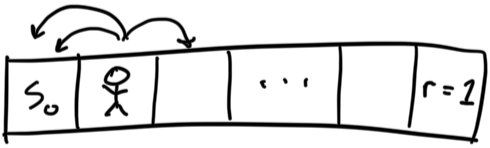
\includegraphics{shared/sparse_reward_mdp.png}

}

\caption{image}

\end{figure}%

There are \(|\mathcal{S}|\) states. The agent starts in the leftmost
state. In every state, there are three possible actions, two of which
move the agent left and one which moves the agent right. The reward
function assigns \(r=1\) to the rightmost cell.

\end{example}

How well would the algorithms we've covered so far do on this problem?
For example, Chapter~\ref{sec-pg} require the gradient to be nonzero in
order to learn. If we never observe any reward, the gradient will always
be zero, and the policy will never change or improve.
Chapter~\ref{sec-fitted_dp} will run into a similar issue: as we
randomly interact with the environment, we will never observe any
reward, and so the reward model simply gives zero for every state-action
pair. In expectation, it would take a computationally infeasible number
of rollouts to observe the reward by chance.

The rest of this chapter will consider ways to \emph{explicitly} add
exploration to these algorithms.

\subsection{Exploration in deterministic
MDPs}\label{exploration-in-deterministic-mdps}

Let us address the exploration problem in a \emph{deterministic} MDP,
that is, where taking action \(a\) in state \(s\) always leads to the
state \(P(s, a) \in \mathcal{S}\). How can we methodically visit every
single state-action pair? In the bandit setting, it was trivial to visit
every arm: just pull each arm once. How might I navigate to a particular
state \(s\) in the MDP setting? Doing so requires planning out a path
from the original state. In fact, solving navigation itself is a complex
RL problem!

\section{Explore-then-exploit (for deterministic
MDPs)}\label{explore-then-exploit-for-deterministic-mdps}

In this simple deterministic setting, the environment never randomly
takes us to unseen states, so our strategy must actively explore new
states.

\begin{definition}[]\protect\hypertarget{def-explore_then_exploit}{}\label{def-explore_then_exploit}

We'll keep a set \(\mathcal{D}\) of all the \((s, a, r, s')\) pairs
we've observed. Each episode, we'll use \(\mathcal{D}\) to construct a
fully known MDP, \(M_{\mathcal{D}}\), in which unseen state-action pairs
are rewarded. We'll then use the planning algorithms from
Section~\ref{sec-opt_dynamic_programming} to reach the unknown states in
\(M_{\mathcal{D}}\).

We assume that every state can be reached from the initial state within
a single episode, and that the action space \(\mathcal{A}\) is fixed.

\begin{enumerate}
\def\labelenumi{\arabic{enumi}.}
\tightlist
\item
  \(\mathcal{D} \gets \emptyset\)
\item
  For \(T = 0, 1, 2, \dots\):

  \begin{enumerate}
  \def\labelenumii{\arabic{enumii}.}
  \tightlist
  \item
    Construct \(M_{\mathcal{D}}\) using \(\mathcal{D}\). That is, the
    state transitions are set to those observed in \(\mathcal{D}\), and
    the reward is set to \(0\) for all state-action pairs in
    \(\mathcal{D}\), and \(1\) otherwise.
  \item
    Execute Section~\ref{sec-opt_dynamic_programming} to compute policy
    \(\widetilde \pi\) Using our known transitions \(\mathcal{D}\),
    compute the shortest path \(\tilde \pi\) to \((s, a)\)
  \item
    Execute \(\tilde \pi\) to visit \((s, a)\) and observe
    \(r = r(s, a), s' = P(s, a)\) \(K \gets K \cup \{ (s, a, r, s') \}\)
    Compute the optimal policy \(\pi^\star\) in the MDP \(K\)
    (e.g.~using policy iteration). \(\pi^\star\).
  \end{enumerate}
\end{enumerate}

\end{definition}

\begin{theorem}[Performance of
explore-then-exploit]\protect\hypertarget{thm-explore_then_exploit_performance}{}\label{thm-explore_then_exploit_performance}

As long as every state can be reached from \(s_0\) within a single
episode, i.e.~\(|\mathcal{S}| \le H\), this will eventually be able to
explore all \(|\mathcal{S}| |\mathcal{A}|\) state-action pairs, adding
one new transition per episode. We know it will take at most
\(|\mathcal{S}| |\mathcal{A}|\) iterations to explore the entire MDP,
after which \(\pi^t = \pi^\star\), incurring no additional regret. For
each \(\pi^t\) up until then, corresponding to the shortest-path
policies \(\tilde \pi\), the value of policy \(\pi^t\) will differ from
that of \(\pi^\star\) by at most \(H\), since the policies will differ
by at most \(1\) reward at each timestep. So,

\[\sum_{t=0}^{T-1} V^\star_0 - V_0^{\pi^t} \le |\mathcal{S}||\mathcal{A}| H.\]

(Note that this MDP and algorithm are deterministic, so the regret is
not random.)

\end{theorem}

\section{Treating an unknown MDP as a MAB}\label{sec-mdp_mab}

We also explored the exploration-exploitation tradeoff in
Chapter~\ref{sec-bandits}. Recall tthat in the MAB setting, we have
\(K\) arms, each of which has an unknown reward distribution, and we
want to learn which of the arms is \emph{optimal}, i.e.~has the highest
mean reward.

One algorithm that struck a good balance between exploration and
exploitation was the \textbf{upper confidence bound} algorithm
Section~\ref{sec-ucb}: For each arm, we construct a \emph{confidence
interval} for its true mean award, and then choose the arm with the
highest upper confidence bound. In summary,

\[k_{t+1} \gets \arg\max_{k \in [K]} \frac{R^{k}_t}{N^{k}_t} + \sqrt{\frac{\ln(2t/\delta)}{2 N^{k}_t}}\]

where \(N_t^k\) indicates the number of times arm \(k\) has been pulled
up until time \(t\), \(R_t^k\) indicates the total reward obtained by
pulling arm \(k\) up until time \(t\), and \(\delta > 0\) controls the
width of the confidence interval. How might we extend UCB to the MDP
case?

Let us formally describe an unknown MDP as an MAB problem. In an unknown
MDP, we want to learn which \emph{policy} is optimal. So if we want to
apply MAB techniques to solving an MDP, it makes sense to think of
\emph{arms} as \emph{policies}. There are
\(K = (|\mathcal{A}|^{|\mathcal{S}|})^H\) deterministic policies in a
finite MDP. Then, ``pulling'' arm \(\pi\) corresponds to using \(\pi\)
to act through a trajectory in the MDP, and observing the total reward.

:::\{attention\} Exercise Which quantity that we have seen so far equals
the mean reward from arm \(\pi\)? :::

Recall that UCB incurs regret \(\tilde{O}(\sqrt{TK})\), where \(T\) is
the number of pulls and \(K\) is the number of arms. So in the
MDP-as-MAB problem, using UCB for \(T\) episodes would achieve regret

\begin{equation}\phantomsection\label{eq-mdp_as_mab}{
\tilde{O}(\sqrt{|\mathcal{A}|^{|\mathcal{S}|H} T})
}\end{equation}

This scales \emph{exponentially} in \(|\mathcal{S}|\) and \(H\), which
quickly becomes intractable. Notably, this method doesn't consider the
information that we gain across different policies. We can illustrate
this with the following example:

\begin{example}[Treating an MDP as a
MAB]\protect\hypertarget{exm-ineffective_mdp}{}\label{exm-ineffective_mdp}

Consider a ``coin MDP'' with two states ``heads'' and ``tails'', two
actions ``Y'' and ``N'', and a time horizon of \(H=2\). The state
transition flips the coin, and doesn't depend on the action. The reward
only depends on the action: Taking action Y gives reward \(1\), and
taking action N gives reward \(0\).

Suppose we collect data from the two constant policies
\(\pi_{\text{Y}}(s) = \text{Y}\) and \(\pi_{\text{N}}(s) = \text{N}\).
Now we want to learn about the policy \(\tilde{\pi}\) that takes action
Y and then N. Do we need to collect data from \(\tilde{\pi}\) to
evaluate it? No: Since the reward only depends on the action, we can
infer its value from our data on the policies \(\pi_{\text{Y}}\) and
\(\pi_{\text{N}}\). However, if we treat the MDP as a bandit in which
\(\tilde{\pi}\) is a new, unknown arm, we ignore the known correlation
between the action and the reward.

\end{example}

\section{UCB-VI}\label{ucb-vi}

The approach above is inefficient: We shouldn't need to consider all
\(|\mathcal{A}|^{|\mathcal{S}| H}\) deterministic policies to achieve
low regret. Rather, all we need to describe the optimal policy is
\(Q^\star\), which has \(H |\mathcal{S}||\mathcal{A}|\) entries to be
learned. Can we borrow ideas from UCB to reduce the regret to a
polynomial in \(|\mathcal{S}|\), \(|\mathcal{A}|\), and \(H\)?

One way to frame the UCB algorithm is that, when choosing arms, we
optimize over a \emph{proxy reward} that is the sum of the estimated
mean reward and an \textbf{exploration term}. In the \textbf{UCB-VI}
algorithm, we will extend this idea to the case of an unknown MDP
\(\mathcal{M}^{?}\) by modelling a proxy MDP \(\widetilde{\mathcal{M}}\)
with a reward function that encourages exploration. Then, we will use DP
to solve for the optimal policy in \(\widetilde{\mathcal{M}}\).

\textbf{Assumptions:} For simplicity, here we assume the reward function
of \(\mathcal{M}^{?}\) is known, so we only need to model the state
transitions, though the rewards can be modelled similarly. We will also
consider the more general case of a \textbf{time-varying} MDP, where the
transition and reward functions may change over time. We take the
convention that \(P_h\) is the distribution of
\(s_{h+1} \mid s_{h}, a_{h}\) and \(r_h\) is applied to \(s_h, a_h\).

At a high level, the UCB-VI algorithm can be described as follows:

\begin{enumerate}
\def\labelenumi{\arabic{enumi}.}
\item
  \textbf{Modelling:} Use previous data to model the transitions
  \(\widehat{P}_0, \dots, \widehat{P}_{H-1}\).
\item
  \textbf{Reward bonus:} Design a reward bonus
  \(b_h(s, a) \in \mathbb{R}\) to encourage exploration, analogous to
  the UCB term.
\item
  \textbf{Optimistic planning:} Use DP to compute the optimal policy
  \(\widehat \pi_h(s)\) in the modelled MDP
\end{enumerate}

\[\tilde{\mathcal{M}} = (\mathcal{S}, \mathcal{A}, \{ \widehat{P}_h\}_{h \in [H]}, \{ r_h+ b_h\}_{h \in [H]}, H).\]

\begin{enumerate}
\def\labelenumi{\arabic{enumi}.}
\setcounter{enumi}{3}
\tightlist
\item
  \textbf{Execution:} Use \(\widehat \pi_h(s)\) to collect a new
  trajectory, and repeat.
\end{enumerate}

We detail each of these steps below. The full definition follows in
Definition~\ref{def-ucb-vi}.

\subsection{Modelling the transitions}\label{modelling-the-transitions}

We seek to approximate
\(P_h(s_{h+1} \mid s_h, a_h) = \frac{\mathbb{P}(s_h, a_h, s_{h+1})}{\mathbb{P}(s_h, a_h)}\).
We can estimate these using their sample probabilities from the dataset.
That is, define

\[\begin{aligned}
    N_h^t(s, a, s') & := \sum_{i=0}^{t-1} \mathbf{1}\left\{ (s_h^i, a_h^i, s_{h+1}^i) = (s, a, s') \right\} \\
    N_h^t(s, a)     & := \sum_{i=0}^{t-1} \mathbf{1}\left\{ (s_h^i, a_h^i) = (s, a) \right\}                \\
\end{aligned}\]

Then we can model

\[\widehat{P}_h^t(s' \mid s, a) = \frac{N_h^t(s, a, s')}{N_h^t(s, a)}.\]

Note that this is also a fairly naive, nonparametric estimator that
doesn't assume any underlying structure of the MDP. We'll see how to
incorporate assumptions about the MDP in the following section.

\subsection{Reward bonus}\label{reward-bonus}

To motivate the reward bonus term \(b_h^t(s, a)\), recall how we
designed the reward bonus term for UCB:

\begin{enumerate}
\def\labelenumi{\arabic{enumi}.}
\item
  We used Hoeffding's inequality to bound, with high probability, how
  far the sample mean \(\widehat \mu_t^k\) deviated from the true mean
  \(\mu^k\).
\item
  By inverting this inequality, we obtained a \((1-\delta)\)-confidence
  interval for the true mean, centered at our estimate.
\item
  To make this bound \emph{uniform} across all timesteps \(t \in [T]\),
  we applied the union bound and multiplied \(\delta\) by a factor of
  \(T\).
\end{enumerate}

We'd like to do the same for UCB-VI, and construct the bonus term such
that \(V^\star_h(s) \le \widehat{V}_h^t(s)\) with high probability.
However, our construction will be more complex than the MAB case, since
\(\widehat{V}_h^t(s)\) depends on the bonus \(b_h^t(s, a)\) implicitly
via DP. We claim that the bonus term that gives the proper bound is

\begin{equation}\phantomsection\label{eq-ucb_vi_bonus}{
b_h^t(s, a) = 2 H \sqrt{\frac{\log( |\mathcal{S}||\mathcal{A}|H T/\delta )}{N_h^t(s, a)}}.
}\end{equation}

We will only provide a heuristic sketch of the proof; see Agarwal et al.
(2022) (Section 7.3) for a full proof.

\begin{refremark}[UCB-VI reward bonus construction]
We aim to show that, with high probability,

\[V_h^\star(s) \le \widehat{V}_h^t(s) \quad \forall t \in [T], h \in [H], s \in \mathcal{S}.\]

We'll do this by bounding the error incurred at each step of DP. Recall
that DP solves for \(\widehat{V}_h^t(s)\) recursively as follows:

\[\widehat{V}_h^t(s) = \max_{a \in \mathcal{A}} \left[ \tilde r^t_h(s, a) + \mathbb{E}_{s' \sim \widehat{P}_h^t(\cdot \mid s, a)} \left[ \widehat{V}_{h+1}^t(s') \right] \right]\]

where \(\tilde r^t_h(s, a) = r_h(s, a) + b_h^t(s, a)\) is the reward
function of our modelled MDP \(\tilde{\mathcal{M}}^t\). On the other
hand, we know that \(V^\star\) must satisfy

\[V^\star_h(s) = \max_{a \in \mathcal{A}} \left[ \tilde r^t_h(s, a) + \mathbb{E}_{s' \sim P^?_h(\cdot \mid s, a)} [V^\star_{h+1}(s')] \right]\]

so it suffices to bound the difference between the two inner
expectations. There are two sources of error:

\begin{enumerate}
\def\labelenumi{\arabic{enumi}.}
\item
  The value functions \(\widehat{V}^t_{h+1}\) v.s. \(V^\star_{h+1}\)
\item
  The transition probabilities \(\widehat{P}_h^t\) v.s. \(P^?_h\).
\end{enumerate}

We can bound these individually, and then combine them by the triangle
inequality. For the former, we can simply bound the difference by \(H\),
assuming that the rewards are within \([0, 1]\). Now, all that is left
is to bound the error from the transition probabilities:

\begin{equation}\phantomsection\label{eq-err}{
\text{error} = \left| \mathbb{E}_{s' \sim \widehat{P}_h^t(\cdot \mid s, a)} \left[ V^\star_{h+1}(s') \right] - \mathbb{E}_{s' \sim P^?_h(\cdot \mid s, a)} \left[ V^\star_{h+1}(s') \right]. \right|
}\end{equation}

Let us bound this term for a fixed \(s, a, h, t\). (Later we can make
this uniform across \(s, a, h, t\) using the union bound.) Note that
expanding out the definition of \(\widehat{P}_h^t\) gives

\[\begin{aligned}
        \mathbb{E}_{s' \sim \widehat{P}_h^t(\cdot \mid s, a)} \left[ V^\star_{h+1}(s') \right] & = \sum_{s' \in \mathcal{S}} \frac{N^t_h(s, a, s')}{N^t_h(s, a)} V^\star_{h+1}(s')                                                     \\
                                                                                   & = \frac{1}{N^t_h(s, a)} \sum_{i=0}^{t-1} \sum_{s' \in \mathcal{S}} \mathbf{1}\left\{ (s_h^i, a_h^i, s_{h+1}^i) = (s, a, s') \right\} V^\star_{h+1}(s') \\
                                                                                   & = \frac{1}{N^t_h(s, a)} \sum_{i=0}^{t-1} \underbrace{\mathbf{1}\left\{ (s_h^i, a_h^i) = (s, a) \right\} V^\star_{h+1}(s_{h+1}^i)}_{X^i}
\end{aligned}\]

since the terms where \(s' \neq s_{h+1}^i\) vanish.

Now, in order to apply Hoeffding's inequality, we would like to express
the second term in Equation~\ref{eq-err} as a sum over \(t\) random
variables as well. We will do this by redundantly averaging over all
desired trajectories (i.e.~where we visit state \(s\) and action \(a\)
at time \(h\)):

\[\begin{aligned}
        \mathbb{E}_{s' \sim P^?_h(\cdot \mid s, a)} \left[ V^\star_{h+1}(s') \right]
         & = \sum_{s' \in \mathcal{S}} P^?_h(s' \mid s, a) V^\star_{h+1}(s')                                                                              \\
         & = \sum_{s' \in \mathcal{S}} \frac{1}{N^t_h(s, a)} \sum_{i=0}^{t-1} \mathbf{1}\left\{ (s_h^i, a_h^i) = (s, a) \right\} P^?_h(s' \mid s, a) V^\star_{h+1}(s') \\
         & = \frac{1}{N^t_h(s, a)} \sum_{i=0}^{t-1} \mathbb{E}_{s_{h+1}^i \sim P^?_{h}(\cdot \mid s_h^i, a_h^i)} X^i.
\end{aligned}
\]

Now we can apply Hoeffding's inequality to
\(X^i - \mathbb{E}_{s_{h+1}^i \sim P^?_{h}(\cdot \mid s_h^i, a_h^i)} X^i\),
which is bounded by \(H\), to obtain that, with probability at least
\(1-\delta\),

\[
\text{error} = \left| \frac{1}{N^t_h(s, a)} \sum_{i=0}^{t-1} \left(X^i - \mathbb{E}_{s_{h+1}^i \sim P^?_{h}(\cdot \mid s_h^i, a_h^i)} X^i \right) \right| \le 2 H \sqrt{\frac{\ln(1/\delta)}{N_h^t(s, a)}}.
\]

Applying a union bound over all
\(s \in \mathcal{S}, a \in \mathcal{A}, t \in [T], h \in [H]\) gives the
\(b_h^t(s, a)\) term above.

\label{rem-ucb_vi_bonus}

\end{refremark}

\subsection{Definition}\label{definition-1}

Putting these parts together, we can define the algorithm as follows:

\begin{definition}[]\protect\hypertarget{def-ucb-vi}{}\label{def-ucb-vi}

TODO

\end{definition}

\(N_h(s, a, s') \gets \sum_{i=0}^{t-1} \mathbf{1}\left\{ (s_h^i, a_h^i, s_{h+1}^i) = (s, a, s') \right\}\)
\(N_h(s, a) \gets \sum_{i=0}^{t-1} \mathbf{1}\left\{ (s_h^i, a_h^i) = (s, a) \right\}\)
\(\widehat P_h\gets \frac{N_h(s, a, s')}{N_h(s, a)}\)
\(b_h(s, a) \gets 2 H \sqrt{\frac{\log( |\mathcal{S}||\mathcal{A}|H T/\delta )}{N_h(s, a)}}\)
\(\tilde{\mathcal{M}} \gets (\mathcal{S}, \mathcal{A}, \{ \widehat{P}_h\}_{h \in [H-1]}, \{ r_h+ b_h\}_{h \in [H-1]}, H)\)
\(\widehat \pi \gets \text{VI}(\tilde{\mathcal{M}})\) Use
\(\widehat \pi_h(s)\) to collect a new trajectory
\((s^t_h, a^t_h, s^t_{h+1})_{h\in [H]}\)

\subsection{Performance of UCB-VI}\label{performance-of-ucb-vi}

How exactly does UCB-VI strike a good balance between exploration and
exploitation? In UCB for MABs, the bonus exploration term is simple to
interpret: It encourages the learner to take actions with a high
exploration term. Here, the policy depends on the bonus term indirectly:
The policy is obtained by planning in an MDP where the bonus term is
added to the reward function. Note that the bonuses \emph{propagate
backwards} in DP, effectively enabling the learner to \emph{plan to
explore} unknown states. This effect takes some further interpretation.

Recall we constructed \(b^t_h\) so that, with high probability,
\(V^\star_h(s) \le \widehat{V}_h^t(s)\) and so

\[V^\star_h(s) - V^{\pi^t}_h(s) \le \widehat{V}_h^t(s) - V^{\pi^t}_h(s).\]

That is, the l.h.s. measures how suboptimal policy \(\pi^t\) is in the
true environment, while the r.h.s. is the difference in the policy's
value when acting in the modelled MDP \(\tilde{\mathcal{M}}^t\) instead
of the true one \(\mathcal{M}^{?}\).

If the r.h.s. is \emph{small}, this implies that the l.h.s. difference
is also small, i.e.~that \(\pi^t\) is \emph{exploiting} actions that are
giving high reward.

If the r.h.s. is \emph{large}, then we have overestimated the value:
\(\pi^t\), the optimal policy of \(\tilde{\mathcal{M}}^t\), does not
perform well in the true environment \(\mathcal{M}^{?}\). This indicates
that one of the \(b_h^t(s, a)\) terms must be large, or some
\(\widehat P^t_h(\cdot \mid s, a)\) must be inaccurate, indicating a
state-action pair with a low visit count \(N^t_h(s, a)\) that the
learner was encouraged to explore.

It turns out that UCB-VI achieves a regret of

\begin{theorem}[UCB-VI
regret]\protect\hypertarget{thm-ucb_vi_regret}{}\label{thm-ucb_vi_regret}

\[\mathbb{E}\left[ \sum_{t=0}^{T-1} \left(V^\star_0(s_0) - V^{\pi^t}_0(s_0) \right) \right] = \tilde{O}(H^2 \sqrt{|\mathcal{S}| |\mathcal{A}| T})\]

\end{theorem}

Comparing this to the UCB regret bound \(\tilde{O}(\sqrt{T K})\), where
\(K\) is the number of arms of the MAB, we see that we've reduced the
number of effective arms from \(|\mathcal{A}|^{|\mathcal{S}|H}\) (in
Equation~\ref{eq-mdp_as_mab}) to \(H^4 |\mathcal{S}||\mathcal{A}|\),
which is indeed polynomial in \(|\mathcal{S}|\), \(|\mathcal{A}|\), and
\(H\), as desired. This is also roughly the number of episodes it takes
to achieve constant-order average regret:

\[\frac{1}{T} \mathbb{E}[\text{Regret}_T] = \tilde{O}\left(\sqrt{\frac{H^4 |\mathcal{S}||\mathcal{A}|}{T}}\right)\]

Note that the time-dependent transition matrix has
\(H |\mathcal{S}|^2 |\mathcal{A}|\) entries. Assuming
\(H \ll |\mathcal{S}|\), this shows that it's possible to achieve low
regret, and achieve a near-optimal policy, while only understanding a
\(1/|\mathcal{S}|\) fraction of the world's dynamics.

\section{Linear MDPs}\label{linear-mdps}

A polynomial dependency on \(|\mathcal{S}|\) and \(|\mathcal{A}|\) is
manageable when the state and action spaces are small. But for large or
continuous state and action spaces, even this polynomial factor will
become intractable. Can we find algorithms that don't depend on
\(|\mathcal{S}|\) or \(|\mathcal{A}|\) at all, effectively reducing the
dimensionality of the MDP? In this section, we'll explore \textbf{linear
MDPs}: an example of a \emph{parameterized} MDP where the rewards and
state transitions depend only on some parameter space of dimension \(d\)
that is independent from \(|\mathcal{S}|\) or \(|\mathcal{A}|\).

\begin{definition}[Linear
MDP]\protect\hypertarget{def-linear_mdp}{}\label{def-linear_mdp}

We assume that the transition probabilities and rewards are
\emph{linear} in some feature vector

\(\phi(s, a) \in \mathbb{R}^d\):

\[\begin{aligned}
        P_h(s' \mid s, a) & = \phi(s, a)^\top \mu^\star_h(s') \\
        r_h(s, a)         & = \phi(s, a)^\top \theta_h^\star
\end{aligned}\]

Note that we can also think of \(P_h(\cdot \mid s, a) = \mu_h^\star\) as
an \(|\mathcal{S}| \times d\) matrix, and think of \(\mu^\star_h(s')\)
as indexing into the \(s'\)-th row of this matrix (treating it as a
column vector). Thinking of \(V^\star_{h+1}\) as an
\(|\mathcal{S}|\)-dimensional vector, this allows us to write

\[\mathbb{E}_{s' \sim P_h(\cdot \mid s, a)}[V^\star_{h+1}(s)] = (\mu^\star_h\phi(s, a))^\top V^\star_{h+1}.\]

The \(\phi\) feature mapping can be designed to capture interactions
between the state \(s\) and action \(a\). In this book, we'll assume
that the feature map
\(\phi : \mathcal{S} \times \mathcal{A} \to \mathbb{R}^d\) and the
reward function (described by \(\theta_h^\star\)) are known to the
learner.

\end{definition}

\subsection{Planning in a linear MDP}\label{planning-in-a-linear-mdp}

It turns out that \(Q^\star_h\) is also linear with respect to this
feature mapping. We can prove this by simply computing it using DP. We
initialize \(V_{H}^\star(s) = 0 \forall s\). Then we iterate:

\[
\begin{aligned}
    Q^\star_h(s, a)  & = r_h(s, a) + \mathbb{E}_{s' \sim P_h(\cdot \mid s, a)} [V^\star_{h+1}(s')]                          \\
                     & = \phi(s, a)^\top \theta_h^\star + (\mu_h^\star \phi(s, a))^\top V^\star_{h+1}               \\
                     & = \phi(s, a)^\top \underbrace{( \theta_h^\star + (\mu_h^\star)^\top  V^\star_{h+1})}_{w_h} \\
    V^\star_h(s)     & = \max_a Q^\star_h(s, a)                                                                       \\
    \pi^\star_h(s) & = \arg\max_a Q^\star_h(s, a)
\end{aligned}
\]

Show that \(Q^\pi_h\) is also linear with respect to \(\phi(s, a)\) for
any policy \(\pi\).

\subsection{UCB-VI in a linear MDP}\label{sec-lin_ucb_vi}

\subsubsection{Modelling the
transitions}\label{modelling-the-transitions-1}

This linear assumption on the MDP will also allow us to model the
unknown dynamics \(P^?_h(s' \mid s, a)\) with techniques from
\textbf{supervised learning} (SL). Recall that SL is useful for
estimating conditional expectations by minimizing mean squared error. We
can rephrase the estimation of \(P^?_h(s' \mid s, a)\) as a
least-squares problem as follows: Write \(\delta_s\) to denote a one-hot
vector in \(\mathbb{R}^{|\mathcal{S}|}\), with a \(1\) in the \(s\)-th
entry and \(0\) everywhere else. Note that

\[\mathbb{E}_{s' \sim P_h(\cdot \mid s, a)} [\delta_{s'}] = P_h(\cdot \mid s, a) = \mu_h^\star \phi(s, a).\]

Furthermore, since the expectation here is linear with respect to
\(\phi(s, a)\), we can directly apply least-squares multi-target linear
regression to construct the estimate

\[\widehat \mu = \arg\min_{\mu \in \mathbb{R}^{|\mathcal{S}| \times d}} \sum_{t=0}^{T-1} \|\mu \phi(s_h^i, a_h^i) - \delta_{s_{h+1}^i} \|_2^2.\]

This has a well-known closed-form solution:

\[\begin{aligned}
    \widehat \mu^\top            & = (A_h^t)^{-1} \sum_{i=0}^{t-1} \phi(s_h^i, a_h^i) \delta_{s_{h+1}^i}^\top \\
    \text{where} \quad A_h^t & = \sum_{i=0}^{t-1} \phi(s_h^i, a_h^i) \phi(s_h^i, a_h^i)^\top + \lambda I
\end{aligned}\]

where we include a \(\lambda I\) term to ensure that the matrix
\(A^t_h\) is invertible. (This can also be derived by adding a
\(\lambda \|\mu\|_{\text{F}}^2\) regularization term to the objective.)
We can directly plug in this estimate into
\(\widehat{P}^t_h(\cdot \mid s, a) = \widehat \mu^t_h \phi(s, a)\).

\subsubsection{Reward bonus}\label{reward-bonus-1}

Now, to design the reward bonus, we can't apply Hoeffding anymore, since
the terms no longer involve sample means of bounded random variables;
Instead, we're incorporating information across different states and
actions. Rather, we can construct an upper bound using \emph{Chebyshev's
inequality} in the same way we did for the LinUCB algorithm in the MAB
setting Section~\ref{sec-lin_ucb}:

\[b^t_h(s, a) = \beta \sqrt{\phi(s, a)^\top (A^t_h)^{-1} \phi(s, a)}, \quad \beta = \tilde O(d H).\]

Note that this isn't explicitly inversely proportional to
\(N_h^t(s, a)\) as in the original UCB-VI bonus term
Equation~\ref{eq-ucb_vi_bonus}. Rather, it is inversely proportional to
the amount that the direction \(\phi(s, a)\) has been explored in the
history. That is, if \(A_h^t\) has a large component in the direction
\(\phi(s, a)\), implying that this direction is well explored, then the
bonus term will be small, and vice versa.

We can now plug in these transition estimates and reward bonuses into
the UCB-VI algorithm Definition~\ref{def-ucb-vi}.

\subsubsection{Performance}\label{performance}

\begin{theorem}[LinUCB-VI
regret]\protect\hypertarget{thm-lin_ucb_vi_regret}{}\label{thm-lin_ucb_vi_regret}

The LinUCB-VI algorithm achieves expected regret

\[\mathbb{E}[\text{Regret}_T] = \mathbb{E}\left[\sum_{t=0}^{T-1} V^\star_0(s_0) - V^{\pi^t}_0(s_0) \right] \le \tilde O(H^2 d^{1.5} \sqrt{T})\]

\end{theorem}

Comparing this to our bound for UCB-VI in an environment without this
linear assumption, we see that we go from a sample complexity of
\(\tilde \Omega(H^4 |\mathcal{S}||\mathcal{A}|)\) to
\(\tilde \Omega(H^4 d^{3})\). This new sample complexity only depends on
the feature dimension and not on the state or action space of the MDP!

\section{Summary}\label{summary-7}

In this chapter, we've explored how to explore in an unknown MDP.

\begin{itemize}
\item
  We first discussed the explore-then-exploit algorithm
  Definition~\ref{def-explore_then_exploit}, a simple way to explore a
  deterministic MDP by visiting all state-action pairs.
\item
  We then discussed how to treat an unknown MDP as a MAB
  Section~\ref{sec-mdp_mab}, and how this approach is inefficient since
  it doesn't make use of relationships between policies.
\item
  We then introduced the UCB-VI algorithm Definition~\ref{def-ucb-vi},
  which models the unknown MDP by a proxy MDP with a reward bonus term
  that encourages exploration.
\item
  Finally, assuming that the transitions and rewards are linear with
  respect to a feature transformation of the state and action, we
  introduced the LinUCB-VI algorithm Section~\ref{sec-lin_ucb_vi}, which
  has a sample complexity independent of the size of the state and
  action spaces.
\end{itemize}

\bookmarksetup{startatroot}

\chapter{Appendix: Background}\label{sec-background}

\begin{center}\rule{0.5\linewidth}{0.5pt}\end{center}

\begin{center}\rule{0.5\linewidth}{0.5pt}\end{center}

\section{O notation}\label{o-notation}

Throughout this chapter and the rest of the book, we will describe the
asymptotic behavior of a function using \(O\) notation.

For two functions \(f(t)\) and \(g(t)\), we say that
\(f(t) \le O(g(t))\) if \(f\) is asymptotically upper bounded by \(g\).
Formally, this means that there exists some constant \(C > 0\) such that
\(f(t) \le C \cdot g(t)\) for all \(t\) past some point \(t_0\).

We say \(f(t) < o(g(t))\) if asymptotically \(f\) grows strictly slower
than \(g\). Formally, this means that for \emph{any} scalar \(C > 0\),
there exists some \(t_0\) such that \(f(t) \le C \cdot g(t)\) for all
\(t > t_0\). Equivalently, we say \(f(t) < o(g(t))\) if
\(\lim_{t \to \infty} f(t)/g(t) = 0\).

\(f(t) = \Theta(g(t))\) means that \(f\) and \(g\) grow at the same rate
asymptotically. That is, \(f(t) \le O(g(t))\) and \(g(t) \le O(f(t))\).

Finally, we use \(f(t) \ge \Omega(g(t))\) to mean that
\(g(t) \le O(f(t))\), and \(f(t) > \omega(g(t))\) to mean that
\(g(t) < o(f(t))\).

We also use the notation \(\tilde O(g(t))\) to hide logarithmic factors.
That is, \(f(t) = \tilde O(g(t))\) if there exists some constant \(C\)
such that \(f(t) \le C \cdot g(t) \cdot \log^k(t)\) for some \(k\) and
all \(t\).

Occasionally, we will also use \(O(f(t))\) (or one of the other symbols)
as shorthand to manipulate function classes. For example, we might write
\(O(f(t)) + O(g(t)) = O(f(t) + g(t))\) to mean that the sum of two
functions in \(O(f(t))\) and \(O(g(t))\) is in \(O(f(t) + g(t))\).

\bookmarksetup{startatroot}

\chapter*{References}\label{references-1}
\addcontentsline{toc}{chapter}{References}

\markboth{References}{References}

\phantomsection\label{refs}
\begin{CSLReferences}{1}{0}
\bibitem[\citeproctext]{ref-agarwal_reinforcement_2022}
Agarwal, Alekh, Nan Jiang, Sham M Kakade, and Wen Sun. 2022.
\emph{Reinforcement {Learning}: {Theory} and {Algorithms}}.

\bibitem[\citeproctext]{ref-baydin_automatic_2018}
Baydin, Atilim Gunes, Barak A. Pearlmutter, Alexey Andreyevich Radul,
and Jeffrey Mark Siskind. 2018. {``Automatic Differentiation in Machine
Learning: A Survey.''} arXiv.
\url{https://doi.org/10.48550/arXiv.1502.05767}.

\bibitem[\citeproctext]{ref-boyd_convex_2004}
Boyd, Stephen, and Lieven Vandenberghe. 2004. \emph{Convex
{Optimization}}. Cambridge University Press.

\bibitem[\citeproctext]{ref-lai_asymptotically_1985}
Lai, T. L, and Herbert Robbins. 1985. {``Asymptotically Efficient
Adaptive Allocation Rules.''} \emph{Advances in Applied Mathematics} 6
(1): 4--22. \url{https://doi.org/10.1016/0196-8858(85)90002-8}.

\bibitem[\citeproctext]{ref-nielsen_neural_2015}
Nielsen, Michael A. 2015. \emph{Neural {Networks} and {Deep Learning}}.
Determination Press.

\bibitem[\citeproctext]{ref-ross_reduction_2010}
Ross, Stéphane, Geoffrey J. Gordon, and J. Bagnell. 2010. {``A
{Reduction} of {Imitation Learning} and {Structured Prediction} to
{No-Regret Online Learning}.''} In \emph{International {Conference} on
{Artificial Intelligence} and {Statistics}}.

\bibitem[\citeproctext]{ref-russell_artificial_2021}
Russell, Stuart J., and Peter Norvig. 2021. \emph{Artificial
Intelligence: A Modern Approach}. Fourth edition. Pearson Series in
Artificial Intelligence. Hoboken: Pearson.

\bibitem[\citeproctext]{ref-schrittwieser_mastering_2020}
Schrittwieser, Julian, Ioannis Antonoglou, Thomas Hubert, Karen
Simonyan, Laurent Sifre, Simon Schmitt, Arthur Guez, et al. 2020.
{``Mastering {Atari}, {Go}, Chess and Shogi by Planning with a Learned
Model.''} \emph{Nature} 588 (7839): 604--9.
\url{https://doi.org/10.1038/s41586-020-03051-4}.

\bibitem[\citeproctext]{ref-schulman_proximal_2017}
Schulman, John, Filip Wolski, Prafulla Dhariwal, Alec Radford, and Oleg
Klimov. 2017. {``Proximal {Policy Optimization Algorithms}.''} arXiv.
\url{https://doi.org/10.48550/arXiv.1707.06347}.

\bibitem[\citeproctext]{ref-silver_mastering_2016}
Silver, David, Aja Huang, Chris J. Maddison, Arthur Guez, Laurent Sifre,
George van den Driessche, Julian Schrittwieser, et al. 2016.
{``Mastering the Game of {Go} with Deep Neural Networks and Tree
Search.''} \emph{Nature} 529 (7587): 484--89.
\url{https://doi.org/10.1038/nature16961}.

\bibitem[\citeproctext]{ref-silver_general_2018}
Silver, David, Thomas Hubert, Julian Schrittwieser, Ioannis Antonoglou,
Matthew Lai, Arthur Guez, Marc Lanctot, et al. 2018. {``A General
Reinforcement Learning Algorithm That Masters Chess, Shogi, and {Go}
Through Self-Play.''} \emph{Science} 362 (6419): 1140--44.
\url{https://doi.org/10.1126/science.aar6404}.

\bibitem[\citeproctext]{ref-silver_mastering_2017}
Silver, David, Julian Schrittwieser, Karen Simonyan, Ioannis Antonoglou,
Aja Huang, Arthur Guez, Thomas Hubert, et al. 2017. {``Mastering the
Game of {Go} Without Human Knowledge.''} \emph{Nature} 550 (7676):
354--59. \url{https://doi.org/10.1038/nature24270}.

\bibitem[\citeproctext]{ref-sussman_functional_2013}
Sussman, Gerald Jay, Jack Wisdom, and Will Farr. 2013. \emph{Functional
Differential Geometry}. Cambridge, MA: The MIT Press.

\bibitem[\citeproctext]{ref-sutton_reinforcement_2018}
Sutton, Richard S., and Andrew G. Barto. 2018. \emph{Reinforcement
Learning: An Introduction}. Second edition. Adaptive Computation and
Machine Learning Series. Cambridge, Massachusetts: The MIT Press.

\bibitem[\citeproctext]{ref-vershynin_high-dimensional_2018}
Vershynin, Roman. 2018. \emph{High-{Dimensional Probability}: {An
Introduction} with {Applications} in {Data Science}}. Cambridge
University Press.

\bibitem[\citeproctext]{ref-williams_simple_1992}
Williams, Ronald J. 1992. {``Simple Statistical Gradient-Following
Algorithms for Connectionist Reinforcement Learning.''} \emph{Machine
Learning} 8 (3): 229--56. \url{https://doi.org/10.1007/BF00992696}.

\end{CSLReferences}




\end{document}
